% =====================================================================
% Section 7: Flow+GAN (flow matching started from the GAN) + ablation summary
% Self-contained. % =====================================================================
% Section 7: Flow+GAN (flow matching started from the GAN) + ablation summary
% Self-contained. % =====================================================================
% Section 7: Flow+GAN (flow matching started from the GAN) + ablation summary
% Self-contained. % =====================================================================
% Section 7: Flow+GAN (flow matching started from the GAN) + ablation summary
% Self-contained. \input{section7_flowgan} from main.tex after \input{section6_srs}.
% Needs the packages main.tex already loads (booktabs, algorithm, algpseudocode,
% listings, xcolor, graphicx). Figures live in figures_cmass/.
% Numbers (updated 2026-09-28, see research_scratch_5.md): summary cross-fid from
% logs/3248394_seedxfid.log (nde_v2, 8 seeds for the main arms) and
% logs/3200801_seedxfid.log (4-seed ablation rows); field cross-fid from
% logs/3248260_fieldev.log (Flow+GAN, 40 epochs), logs/3203212_fieldev.log (20 epochs)
% and the other *_fieldev.log files; scale-by-scale from scratch/why/coh.py
% (COH_SPLIT=test, 200 test boxes); posterior shifts from scratch/why/post_diag_any.py
% (logs/3249151_postdiag.log, logs/3251464_postdiag.log); PQMass, bispectrum and halo
% counts from logs/*_tier1.log; calibration from logs/3251512_spread.log; figures from
% flow_matching/plot_sec7.py. LR here is CHARM (section6_srs.tex calls it FastPM,
% which is wrong).
% =====================================================================

\definecolor{ablgood}{HTML}{1B7F1B}
\newcommand{\abgood}[1]{\textcolor{ablgood}{\textbf{#1}}}

\section{Flow+GAN: Flow Matching Started from the GAN}
\label{sec:flowgan}

This section documents the third model in this work at the same level of detail
as \S\ref{sec:srs}. \S\ref{sec:srs} corrects the LR halo count field with a
styled GAN. The GAN makes the field look like HR, but it is deterministic, and
it biases the summary-level cosmology posterior. Here we keep that GAN and add a
conditional \textbf{flow-matching} model on top of it. The flow starts from the
GAN's output plus noise and learns to turn it into a sample of the HR field. We
call the combined model \textbf{Flow+GAN}. The section ends with a table of
every model and ablation we ran on this data (\S\ref{sec:flowgan-ablations}).

\paragraph{Goal.} The goal is the same as in \S\ref{sec:srs}. At inference the
model sees only the cheap LR field and must produce an SR field that behaves like
HR. We grade it the same way: a posterior trained on SR fields is applied to HR
fields, and we measure how far its answer is from a posterior trained on HR
(cross-fidelity KL). HR is used only for training and grading.

\paragraph{Why a new model: what the GAN and a plain flow get wrong.} Two
findings from the previous section and its follow-ups motivate this design.
\begin{itemize}
  \item \textbf{The GAN is deterministic and tilts the power spectrum.} Its
  learned noise strength is about $2\times10^{-4}$, so ten noise draws give the
  same field. Its $L_1$ term pulls each voxel toward the conditional median.
  This shrinks the large-scale contrast (about $5\%$ less power at $k<0.06\,h\,\mathrm{Mpc}^{-1}$)
  and adds $1$ to $3\%$ power at high $k$. A posterior reads this tilt as a
  shift in $\sigma_8$: on HR test boxes the GAN-trained posterior's $\sigma_8$ mean
  is off by about one HR posterior width. That is why the deployed GAN's summary
  cross-fidelity KL ($0.202$) is worse than raw LR ($0.049$). One fixed per-$k$
  calibration curve on the GAN's training $P(k)$ brings it to $0.068$, which
  shows the problem is this tilt, not missing information.
  \item \textbf{A plain flow samples, but loses the large scales.} A flow that
  starts from pure Gaussian noise (``Flow'' below) has no $\sigma_8$ bias and
  reaches $0.087$. But it rebuilds every scale from noise, including the largest
  ones, which LR already gets right. Its large-scale power scatters more from box
  to box than LR's. Its coherence with HR at $k\approx0.125$ falls below LR's.
  Its predictions are also too narrow: HR usually falls outside the spread of its
  draws (spread-skill ratio $0.20$, ideal $1$).
\end{itemize}
Flow+GAN takes the part each model gets right. The GAN supplies the large-scale
structure and a best guess. The flow adds only what the best guess cannot
predict, and it adds it as a sample, not as a mean. This follows residual
diffusion for downscaling (CorrDiff, Mardani et al.\ 2023, arXiv:2309.15214),
stochastic flow matching for super-resolution (Fotiadis et al.\ 2024,
arXiv:2410.19814), and stochastic interpolants with a data-dependent start
(Albergo et al.\ 2023, arXiv:2310.03725).

\paragraph{Terminology.} \textbf{GAN} means the deployed generator of
\S\ref{sec:srs}: Arm A (pad $0$), power-spectrum loss off, trained with correct
cosmology labels, run at the fiducial cosmology (tag \texttt{Afixfid}).
\textbf{Flow} means the pure-noise flow matcher trained on $64^3$ patches (tag
\texttt{fm\_gauss\_nodq}). \textbf{Flow+GAN} is the model of this section. As in
\S\ref{sec:srs}, we use LR/LF and HR/HF interchangeably.

\subsection{Data Preprocessing}
\textit{Source: \texttt{cmass-ili}; loaders \texttt{flow\_matching/data.py}
(\texttt{FullBoxDataset}), model space \texttt{flow\_matching/space.py}.}

\paragraph{Input.} The data is the same as in \S\ref{sec:srs}: $2000$ paired
halo count grids of $128^3$ cells on a periodic $1000\,h^{-1}\mathrm{Mpc}$ box at
$z=0.5$, with LR from CHARM and HR from Quijote N-body, and the same
$1600/200/200$ train/validation/test split. One extra input is new. Before
training, we run the GAN once on every one of the $2000$ LR boxes, at the
fiducial cosmology, and store its output (\texttt{sr\_fields/Afix\_fiducial}).
The GAN is frozen from here on; it is not trained further.

\paragraph{Model space.} The flow works on a standardised log count,
\begin{equation}
  y = \frac{\log(1+n) - \mu}{s}, \qquad
  n = \mathrm{round}\big(\exp(s\,y+\mu) - 1\big) \ \ \text{clamped to } [0, 200],
  \label{eq:fg-space}
\end{equation}
where $\mu=0.152$ and $s=0.359$ are the mean and standard deviation of
$\log(1+n_\text{HR})$ over $50$ training boxes. The LR field, the GAN field and
the HR target all use this same map. We do \emph{not} dequantise (add uniform
noise to the integer counts before the log). An earlier flow that did so
(\texttt{fm\_gauss}) needed a floor decoder, and noise near the empty-cell
boundary made spurious halos: about $9\%$ too many halos, and a summary KL of
$0.244$. The rounding decoder in Eq.~\ref{eq:fg-space} does not have this bias.
Power spectra are computed exactly as in \S\ref{sec:srs}, on the physical-count
overdensity $\delta = n/\bar n - 1$ with the per-box mean.

\subsection{Data Pipeline (full box, no patches)}
\textit{Located in: \texttt{flow\_matching/data.py},
\texttt{flow\_matching/augment.py}, \texttt{flow\_matching/train\_fm.py}.}

Unlike the GAN and the earlier flows, Flow+GAN is trained and sampled on the
\textbf{whole $128^3$ box at once}. The patch pipeline of \S\ref{sec:srs} cuts
each box into eight $64^3$ cores. For a model that draws fresh noise per patch,
this matters: each patch gets its own noise. Modes longer than a patch are then
re-drawn independently in each patch, and the circular padding treats a patch as
periodic when it is not. Sampling the old patch-trained flow on the full box
already raised its coherence with HR at $k=0.125$ from $0.36$ to $0.67$. The
velocity network is fully convolutional with circular padding, so it runs on
$128^3$ without change, and the box is truly periodic, so circular padding is
exact.

Each training item is one box: the LR counts, the HR counts and the GAN output,
all $128^3$. Two augmentations are applied identically to all three fields:
\begin{itemize}
  \item \textbf{Random periodic shift.} The three fields are rolled by the same
  random offset along each axis. Because the box is periodic this is an exact
  symmetry, and it stops the network from learning fixed positions.
  \item \textbf{Cube symmetries.} One of the $48$ rotations and reflections of
  the cube (\texttt{--aug full48}).
\end{itemize}

\begin{table}[t]
\centering
\caption{Notation for the Flow+GAN pipeline.}
\label{tab:fg-notation}
\begin{tabular}{llp{7.0cm}}
\toprule
Symbol & Value & Meaning \\
\midrule
$N$ & $128$ & box side in voxels (the model sees the whole box) \\
$y_\text{LR},\,y_\text{GAN},\,y_\text{HR}$ & $(1,128^3)$ & LR, GAN and HR fields in model space (Eq.~\ref{eq:fg-space}) \\
$\sigma_z$ & $0.920$ & RMS of $y_\text{HR}-y_\text{GAN}$ over $50$ training boxes ($64^3$ patches) \\
$t$ & $[0,1]$ & flow time; $t{=}0$ is the noisy GAN field, $t{=}1$ is HR \\
$x_t$ & $(1,128^3)$ & point on the straight path between source and target \\
$v_\phi$ & $17.4$M params & velocity network (3D UNet) \\
\bottomrule
\end{tabular}
\end{table}

\subsection{Model: Input/Output Specification}
\textit{Implementation: \texttt{flow\_matching/interpolant.py}
(\texttt{Interpolant}, source \texttt{gan\_white}),
\texttt{flow\_matching/unet3d.py}.}

\paragraph{The path.} Flow matching learns a velocity field that carries a
\emph{source} sample $x_0$ to a \emph{target} sample $x_1$ along a straight line.
For Flow+GAN the source is the GAN's field plus white noise at the size of the
GAN's typical error, and the target is HR:
\begin{equation}
  x_0 = y_\text{GAN} + \sigma_z\,\boldsymbol\epsilon,\quad
  \boldsymbol\epsilon\sim\mathcal N(0,I), \qquad
  x_1 = y_\text{HR}, \qquad
  x_t = (1-t)\,x_0 + t\,x_1 .
  \label{eq:fg-path}
\end{equation}
The velocity along this line is constant, $x_1-x_0$. The network is trained to
predict it:
\begin{equation}
  \mathcal L_\text{FM} \;=\; \mathbb E_{t,\,\boldsymbol\epsilon,\,\text{box}}
    \big\lVert v_\phi\big(x_t,\,t,\,[y_\text{LR},\,y_\text{GAN}]\big) - (x_1 - x_0)\big\rVert_2^2 ,
  \qquad t\sim\mathcal U[0,1].
  \label{eq:fg-loss}
\end{equation}
This is the only loss. There is no adversarial term, no $L_1$ term and no
power-spectrum term.

\paragraph{Why start from the GAN.} With a pure-noise source ($x_0\sim\mathcal
N(0,I)$) the flow must create every scale, including the large scales that LR
and the GAN already get right. Starting at the GAN field means the flow's job is
only the residual $y_\text{HR}-y_\text{GAN}$, whose size is $\sigma_z$. The noise
$\sigma_z\boldsymbol\epsilon$ is what makes the model stochastic: with
$\sigma_z=0$ the flow would be a deterministic map and could return only one
field per LR box, which is the GAN's failure again. The noise is white, so it
has little power at large scales, and the large-scale modes of the start point
are essentially the GAN's.

\paragraph{Conditioning.} The network sees the current state $x_t$ and two
conditioning channels, the LR field and the GAN field, concatenated as input
channels ($3$ input channels in total). It does \emph{not} see the cosmology
vector: the flow is $\theta$-independent. The only $\theta$ in the pipeline is
the fixed fiducial value given to the frozen GAN, so no per-box cosmology can
leak into the SR fields.

\begin{table}[t]
\centering
\caption{Tensors consumed/produced by the velocity network for one box (batch
dimension omitted).}
\label{tab:fg-io}
\begin{tabular}{lll}
\toprule
Symbol & Shape & Meaning \\
\midrule
$x_t$ & $(1,128,128,128)$ & current state on the path (Eq.~\ref{eq:fg-path}) \\
$y_\text{LR}$ & $(1,128,128,128)$ & LR field, model space (conditioning) \\
$y_\text{GAN}$ & $(1,128,128,128)$ & frozen GAN output, model space (conditioning and start point) \\
$t$ & scalar & flow time, sinusoidal embedding \\
$v_\phi(\cdot)$ & $(1,128,128,128)$ & predicted velocity \\
\bottomrule
\end{tabular}
\end{table}

\paragraph{Velocity network.} $v_\phi$ is a 3D UNet with $17.4$M parameters.
\begin{enumerate}
  \item Every convolution is $3{\times}3{\times}3$ with circular padding, so the
  network is exactly shift-equivariant on the periodic box.
  \item Four levels at full, $1/2$, $1/4$ and $1/8$ resolution with channel
  widths $32\cdot(1,2,4,4)$, two residual blocks per level, GroupNorm, and one
  self-attention block at the coarsest level for global context.
  \item The time $t$ enters through a sinusoidal embedding and an MLP that sets a
  per-channel scale and shift after each GroupNorm (FiLM).
  \item The last convolution is initialised to zero, so the initial velocity is
  about $0$.
\end{enumerate}
Training keeps an exponential moving average (EMA, decay $0.999$) of the weights;
validation and sampling use the EMA weights.

\subsection{Training Step}
\textit{Located in: \texttt{flow\_matching/train\_fm.py}.}

\begin{algorithm}[H]
\caption{Flow+GAN training step (one box)}
\label{alg:fg-train}
\begin{algorithmic}[1]
\Require LR counts $\mathbf L$, HR counts $\mathbf H$, frozen GAN output $\mathbf G$ (all $128^3$), $\sigma_z$
\State draw one random periodic shift and one of $48$ cube symmetries; apply both to $\mathbf L,\mathbf H,\mathbf G$
\State $y_\text{LR},y_\text{HR},y_\text{GAN}\gets$ Eq.~\ref{eq:fg-space} applied to $\mathbf L,\mathbf H,\mathbf G$
\State $\boldsymbol\epsilon\sim\mathcal N(0,I)$, \ $t\sim\mathcal U[0,1]$
\State $x_0\gets y_\text{GAN}+\sigma_z\boldsymbol\epsilon$, \ $x_t\gets(1-t)x_0+t\,y_\text{HR}$
\State $\mathcal L\gets\big\lVert v_\phi(x_t,t,[y_\text{LR},y_\text{GAN}])-(y_\text{HR}-x_0)\big\rVert^2$ \Comment{mean over voxels}
\State update $\phi$ (AdamW, linear warm-up $500$ steps, grad-clip $1$, bf16); update EMA
\end{algorithmic}
\end{algorithm}

\paragraph{Validation and checkpoint selection.} After each epoch we generate
$2$ draws for each of the first $16$ validation boxes ($16$ Heun steps) and
compute, in $\log(1+n)$ space: the $L_1$ error per voxel, the fair
\textbf{CRPS} of the $2$-draw ensemble, the spread between draws, the
total-count error, and the $P(k)$ RMS against HR. For $K$ draws $s_1,\dots,s_K$
and the true value $h$, the per-voxel fair CRPS is
\begin{equation}
  \mathrm{CRPS} = \frac1K\sum_{i}|s_i-h| - \frac{1}{2K(K-1)}\sum_{i\neq j}|s_i-s_j| .
  \label{eq:fg-crps}
\end{equation}
The first term rewards draws close to HR; the second rewards draws that differ
from each other. So CRPS, unlike $L_1$, does not favour a blurred mean field.
\texttt{best.pt} is the epoch with the lowest validation CRPS. We fixed this rule
before training. $P(k)$ is only a check: it is never trained on and never used
to select.

\subsection{Inference}
\textit{Located in: \texttt{flow\_matching/sample\_fm.py},
\texttt{flow\_matching/common.py} (\texttt{generate\_box}).}

For one box: run the frozen GAN on LR (already stored), build the start point
$x_0$, integrate the learned velocity from $t=0$ to $t=1$ with Heun's
second-order method, and map back to counts. The noise is seeded by the box index
and draw number, so every output can be reproduced.

\begin{algorithm}[H]
\caption{Flow+GAN inference (one box, one draw)}
\label{alg:fg-infer}
\begin{algorithmic}[1]
\Require LR box $\mathbf L$, GAN output $\mathbf G$, trained $v_\phi$ (EMA), $\sigma_z$, steps $S{=}32$, seed
\State $y_\text{LR},y_\text{GAN}\gets$ Eq.~\ref{eq:fg-space}; \ $x\gets y_\text{GAN}+\sigma_z\boldsymbol\epsilon$ \Comment{seeded $\boldsymbol\epsilon$}
\For{$i=0,\dots,S-1$} \Comment{$t_i=i/S$, $\Delta t = 1/S$}
  \State $v_0\gets v_\phi(x,t_i,[y_\text{LR},y_\text{GAN}])$
  \If{$i<S-1$}
    \State $v_1\gets v_\phi(x+\Delta t\,v_0,\,t_{i+1},[y_\text{LR},y_\text{GAN}])$; \ $x\gets x+\tfrac12\Delta t\,(v_0+v_1)$ \Comment{Heun}
  \Else
    \State $x\gets x+\Delta t\,v_0$ \Comment{Euler on the last step}
  \EndIf
\EndFor
\State \Return $\mathrm{round}\big(\exp(s\,x+\mu)-1\big)$, clamped to $[0,200]$ \Comment{integer counts}
\end{algorithmic}
\end{algorithm}

\paragraph{No stitching.} Because the whole box is generated at once, there are
no cores, no halo and no seams. The stitching step of \S\ref{sec:srs} does not
apply.

\subsection{Evaluation}
\label{sec:fg-eval}
\textit{Located in: \texttt{evaluate.py}, \texttt{inference/nde.py},
\texttt{analysis/seed\_xfid\_check.py}, \texttt{eval\_field\_crossfid.py},
\texttt{scratch/why/coh.py}, \texttt{flow\_matching/plot\_sec7.py}.}

We use the metrics of \S\ref{sec:srs-eval}: the power spectrum, the transfer
$T(k)=P_X/P_\text{HR}$, the cross-coherence $r(k)$ with HR
(Eq.~\ref{eq:srs-Tr}), and cross-fidelity KL (Eq.~\ref{eq:srs-kl}) at two levels.
One thing changed in the summary-level protocol, so the numbers below are not
directly comparable to Table~\ref{tab:srs-corrected}:
\begin{itemize}
  \item \textbf{Summary level (protocol v2).} The NDE input is $\log_{10}P(k)$ in
  $29$ bins. The three lowest of the original $32$ bins contain no Fourier modes,
  and we now drop them. We train $8$ NDE seeds for each of the main sources (HR,
  LR, GAN, Flow and every Flow+GAN checkpoint) and $4$ for the other ablations.
  For seed $s$ we compare $q_X^{(s)}$ with $q_\text{HR}^{(s)}$ on the $200$ HR test
  boxes and report the mean $\pm$ standard deviation over seeds. The HR floor is
  the KL between independently trained HR posteriors. This per-seed protocol is
  stricter than the ensemble protocol of \S\ref{sec:srs-correction}: LR is $0.049$
  here versus $0.032$ there. The ranking of the GAN arms is the same under both.
  \item \textbf{Field level.} Unchanged from \S\ref{sec:srs-correction}: a 3D CNN
  posterior on the full box, $3$ CNN seeds trained on SR, evaluated on HR test
  boxes against $6$ HR-trained reference CNNs. The same $8$ LR CNNs and $6$ HR
  CNNs are reused for every arm.
\end{itemize}

\subsection{Best-Run Configuration}
\textit{Run script: \texttt{scratch/why/train\_v2\_1gpu.slurm} (resumes automatically
from \texttt{last.pt}, so the same script ran epochs $0$ to $19$ and $20$ to $39$); checkpoint
\texttt{models/Flow+GAN/best\_crps40\_epoch39.pt}; sampling \texttt{scratch/why/gen\_v2.slurm}.}

\begin{lstlisting}[language=bash]
--source gan_white                        # python -m flow_matching.train_fm
--extra-dir sr_fields/Afix_fiducial     # frozen GAN output: start point + 2nd cond channel
--full-box --roll --aug full48          # whole periodic box, random shift + 48 symmetries
--no-dequant                            # round decoder
--base-ch 32 --ch-mult 1,2,4,4 --attn-levels 3    # 17.4M-param UNet
--lr 1e-4 --warmup 500 --ema 0.999 --grad-clip 1.0 --amp bf16
--epochs 40 --select crps --val-max-sims 16 --val-draws 2 --val-steps 16
# sampling: --steps 32 --method heun (full box, EMA weights, seeded per box)
\end{lstlisting}

The run used one GH200 GPU (about $13.5$ minutes per epoch, batch of one box).
Epochs are numbered from $0$, as in the training log. We first stopped the run
after $20$ epochs, because validation CRPS had been flat since epoch $11$; that
run's CRPS-best checkpoint was epoch $15$. The validation $P(k)$ error was still
falling, so we resumed the same run, with the same recipe, weights, EMA and optimizer state,
to the planned $40$ epochs. Before looking at any test result we fixed which
checkpoints to report: the CRPS-best one (epoch $38$, the one we use below) and the
final one (epoch $39$). Validation at those epochs:

\begin{center}
\begin{tabular}{lccccc}
\toprule
model & $L_1$/voxel & CRPS & spread & count error & $P(k)$ RMS \\
\midrule
Flow+GAN, epoch 15 (first $20$ epochs) & $0.146$ & $0.0749$ & $0.071$ & $+0.2\%$ & $0.059$ \\
Flow+GAN, epoch 38 (CRPS-best of $40$) & $0.144$ & $\mathbf{0.0740}$ & $0.070$ & $-1.6\%$ & $\mathbf{0.052}$ \\
Flow+GAN, epoch 39 (final) & $0.143$ & $\mathbf{0.0740}$ & $0.069$ & $-1.5\%$ & $0.053$ \\
Flow from noise, full box (control) & $0.195$ & $0.100$ & -- & $+3.2\%$ & $0.084$ \\
\bottomrule
\end{tabular}
\end{center}
The control row is the same recipe with a pure-noise source instead of the GAN,
read at epoch $7$ to $8$ for comparison (its later epochs were unstable). Flow+GAN
is better on every validation metric. The second $20$ epochs improve CRPS only
slightly ($0.0749\to0.0740$, flat from epoch $30$), but they reduce the $P(k)$ error
($0.059\to0.052$), even though $P(k)$ is not in the loss. The validation count error
is measured on only $16$ boxes and moves by about $1\%$ from epoch to epoch.

\subsection{Results}
\label{sec:fg-results}

\paragraph{1. Power spectrum: the tilt is gone.} Figure~\ref{fig:fg-pk} and
Table~\ref{tab:fg-scale} compare the power spectrum and cross-coherence of LR,
the GAN, the Flow and Flow+GAN against HR. Flow+GAN's median power is within
$1.4\%$ of HR at every scale ($0.986$ to $1.009$). The median transfer deviates
from $1$ by $1.1\%$ RMS, against $2.7\%$ for raw LR, $4.4\%$ for the GAN and
$6.1\%$ for the Flow. The GAN's pattern (too little power at large scales, too
much at small scales) is removed, and so is the Flow's $3$ to $4\%$ deficit at
most scales. The cross-coherence with HR is above LR at every scale except the
largest ($r=0.76$ vs $0.51$ at $k\approx0.125$, $0.34$ vs $-0.13$ at
$k\approx0.35$). It stays below the GAN's, which is expected: a sampler draws
the unpredictable small-scale structure fresh, while the GAN returns its
single best guess.

\begin{figure}[t]
\centering
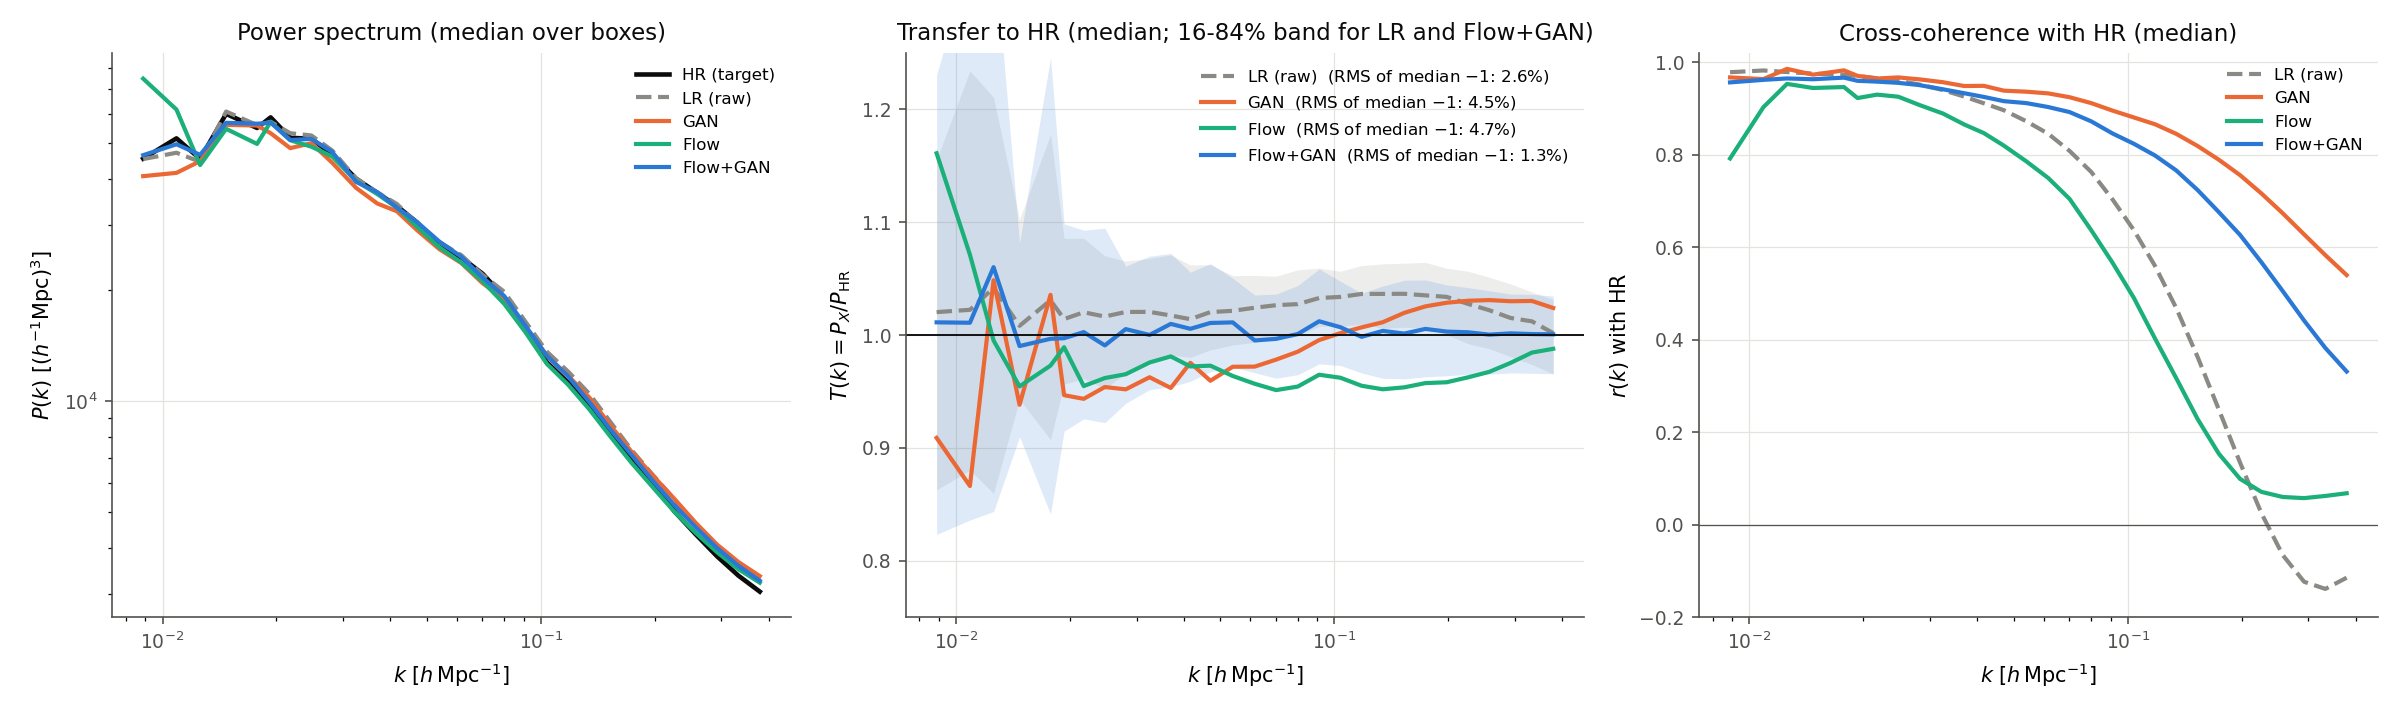
\includegraphics[width=\linewidth]{figures_cmass/pk_panel_box_flowgan.png}
\caption{Full-box diagnostic on $100$ validation boxes. Flow+GAN has no
test-split fields yet, and the first $16$ validation boxes (in sorted order)
were used for checkpoint selection, so we use the next $100$.
\textbf{Left:} median $P(k)$ of HR, LR, GAN, Flow and Flow+GAN.
\textbf{Middle:} transfer $T(k)=P_X/P_\text{HR}$, median, with the 16 to 84
percentile band for LR and Flow+GAN; the legend gives the RMS deviation of the
median from $1$. The GAN (orange) is low at large scales and high at small
scales; the Flow (green) is low at all scales; Flow+GAN (blue) stays on $1$.
\textbf{Right:} cross-coherence $r(k)$ with HR. Flow+GAN is above LR from
$k\approx0.05$ onward and below the deterministic GAN.}
\label{fig:fg-pk}
\end{figure}

\begin{table}[t]
\centering
\caption{Scale by scale, the first $100$ validation boxes, in wide $k$ bands
centred on the listed values. $P/P_\text{HR}$: median power
ratio to HR ($1$ is right). Scatter: box-to-box standard deviation of that ratio
(LR is the reference). $r$: median cross-coherence with HR ($1$ is best).}
\label{tab:fg-scale}
\small
\begin{tabular}{l cccc cc cccc}
\toprule
 & \multicolumn{4}{c}{$P/P_\text{HR}$ median} & \multicolumn{2}{c}{scatter} & \multicolumn{4}{c}{$r$ with HR} \\
\cmidrule(lr){2-5}\cmidrule(lr){6-7}\cmidrule(lr){8-11}
$k$ [$h\,\mathrm{Mpc}^{-1}$] & $0.013$ & $0.042$ & $0.125$ & $0.35$ & $0.013$ & $0.125$ & $0.013$ & $0.042$ & $0.125$ & $0.35$ \\
\midrule
LR (raw)  & $1.009$ & $1.017$ & $1.037$ & $1.007$ & $\mathbf{0.20}$ & $0.34$ & $\mathbf{0.975}$ & $0.908$ & $0.508$ & $-0.126$ \\
GAN       & $0.949$ & $0.962$ & $1.010$ & $1.029$ & $\mathbf{0.20}$ & $0.34$ & $0.974$ & $\mathbf{0.944}$ & $\mathbf{0.850}$ & $\mathbf{0.559}$ \\
Flow      & $1.057$ & $0.970$ & $0.959$ & $0.989$ & $0.40$ & $\mathbf{0.32}$ & $0.907$ & $0.837$ & $0.358$ & $0.062$ \\
Flow+GAN  & $\mathbf{0.986}$ & $\mathbf{1.004}$ & $\mathbf{0.998}$ & $\mathbf{1.009}$ & $0.29$ & $0.35$ & $0.964$ & $0.921$ & $0.760$ & $0.339$ \\
\bottomrule
\end{tabular}
\end{table}

\paragraph{2. Cross-fidelity: Flow+GAN matches LR at the summary level and stays near the floor at the field level.}
Figure~\ref{fig:fg-crossfid} and Table~\ref{tab:fg-crossfid} give the goal
metric. At the summary level the $40$-epoch Flow+GAN reaches $0.047\pm0.008$,
against $0.049\pm0.010$ for raw LR. Compared seed by seed (same NDE seed, same HR
reference posterior), the difference from LR averages $-0.001$. It is the first
SR model that is not worse than LR at the summary level: the GAN is at $0.202$
and the Flow at $0.087$. The final checkpoint (epoch $39$) gives $0.055\pm0.011$,
also equal to LR within noise. At the field level Flow+GAN reaches $0.027\pm0.011$,
close to the HR floor ($0.019$), while the LR-trained CNN posterior does not
transfer reliably ($0.47\pm0.78$).

Two cautions apply. First, epochs $38$ and $39$ are neighbouring checkpoints of one
run, yet their summary KLs differ by $0.008$, about one seed standard deviation.
So the fair claim is that Flow+GAN is equal to LR within noise, not that it beats
LR. Second, the $20$-epoch model (epoch $15$) was at $0.065\pm0.011$. The
improvement from longer training is therefore real but modest, and it is of the
same order as the checkpoint-to-checkpoint noise.

\begin{figure}[t]
\centering
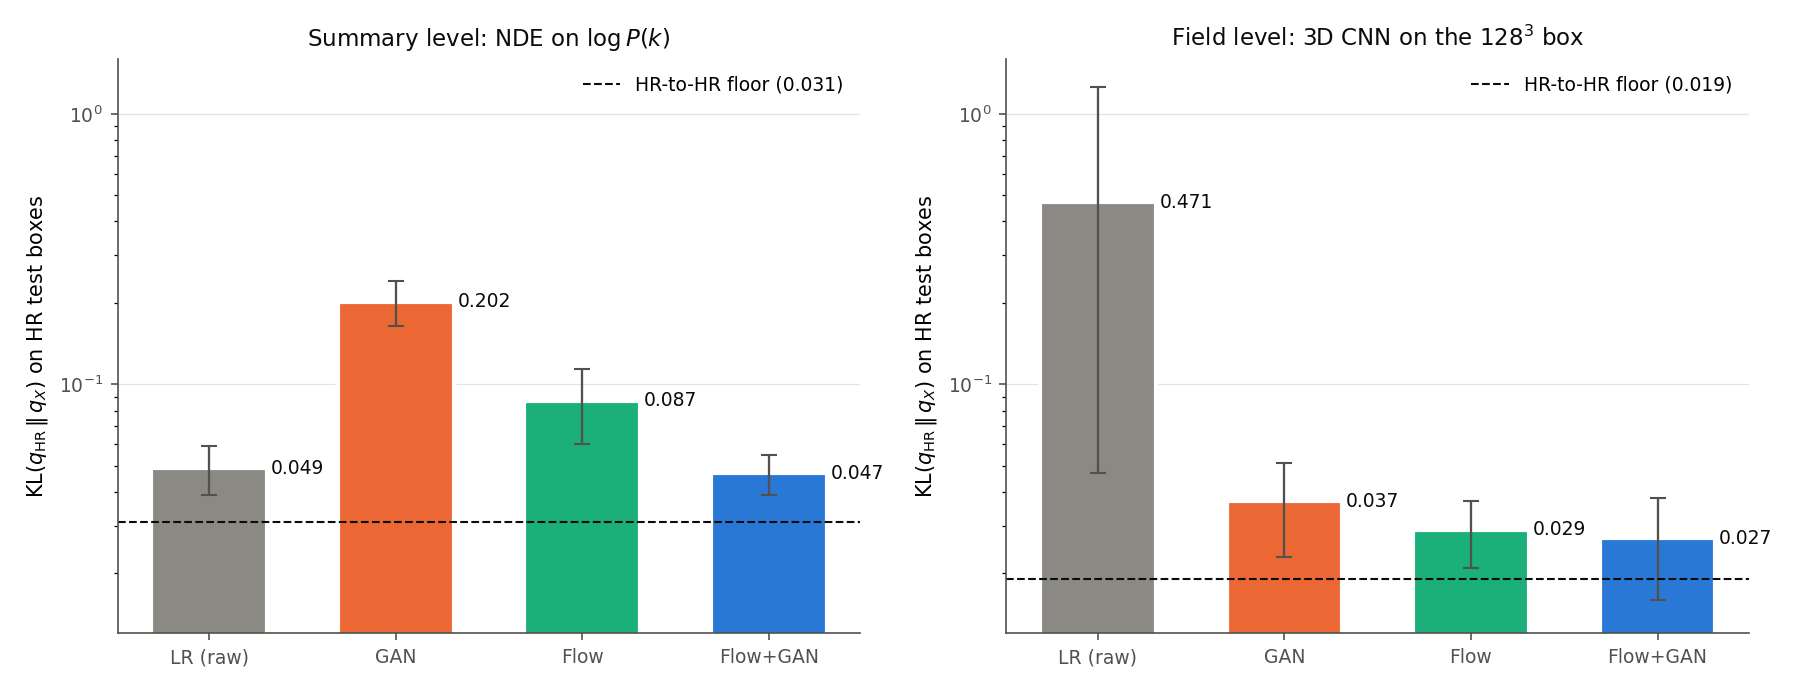
\includegraphics[width=0.95\linewidth]{figures_cmass/crossfid_flowgan.png}
\caption{Cross-fidelity KL to HR (log scale, lower is better), posterior trained
on source $X$ and applied to the $200$ HR test boxes. Dashed: HR-to-HR floor.
Flow+GAN is the $40$-epoch model (CRPS-best checkpoint).
\textbf{Left:} summary level ($P(k)$ NDE, protocol v2, mean $\pm$ std over $8$
seeds). Flow+GAN ($0.047$) equals raw LR ($0.049$); the GAN is at $0.202$ and the
Flow at $0.087$. \textbf{Right:} field level (3D CNN). All three SR models are
near the floor, Flow+GAN ($0.027$) closest; LR does not transfer reliably.}
\label{fig:fg-crossfid}
\end{figure}

\begin{table}[t]
\centering
\caption{Cross-fidelity KL to HR, lower is better. Summary: protocol v2, mean
$\pm$ std over $8$ NDE seeds, $200$ HR test boxes. Field: mean $\pm$ std over
HR-reference $\times$ SR-replicate pairs. Best SR value per column in bold.}
\label{tab:fg-crossfid}
\begin{tabular}{lcc}
\toprule
source & summary $P(k)$ & field (CNN) \\
\midrule
LR (raw, control) & $0.049\pm0.010$ & $0.471\pm0.782$ \\
GAN (deployed)    & $0.202\pm0.038$ & $0.037\pm0.014$ \\
Flow (noise start, patches) & $0.087\pm0.027$ & $0.029\pm0.008$ \\
Flow+GAN, epoch 15 ($20$-epoch run) & $0.065\pm0.011$ & $\mathbf{0.024\pm0.009}$ \\
Flow+GAN, epoch 38 (CRPS-best of $40$) & $\mathbf{0.047\pm0.008}$ & $0.027\pm0.011$ \\
Flow+GAN, epoch 39 (final) & $0.055\pm0.011$ & $0.027\pm0.015$ \\
\midrule
HR floor          & $0.031\pm0.009$ & $0.019$ \\
\bottomrule
\end{tabular}
\end{table}

\paragraph{3. Why it works: the posterior shifts.} Table~\ref{tab:fg-s8}
measures directly how each SR-trained posterior differs from the HR-trained one.
For each HR test box and seed we take the SR-trained posterior mean minus the
HR-trained posterior mean, in units of the HR posterior's standard deviation. We
report the mean over boxes (bias) and the standard deviation over boxes (scatter),
averaged over the $8$ seeds, for the two parameters the $P(k)$ posterior
constrains best, $\Omega_m$ and $\sigma_8$. The GAN's problem is a single one:
its $\sigma_8$ is biased by a full posterior width. After $20$ epochs Flow+GAN has
no such bias beyond LR's own ($+0.23$ vs $+0.18$), but its $\Omega_m$ scatter is
larger than LR's ($0.22$ vs $0.17$). After $40$ epochs the $\sigma_8$ bias is gone
($-0.01$) and the $\Omega_m$ scatter has dropped to $0.18$, close to LR. The same
pattern holds for $n_s$ (scatter $0.34\to0.30$, LR $0.27$). These are the changes
that close the summary gap. The per-box scatter of $\sigma_8$ was never the
problem: it is at LR's level for every Flow+GAN checkpoint. The final checkpoint
(epoch $39$) has a $\sigma_8$ bias of $+0.17$, which is again LR's level, which
shows how much this quantity moves between neighbouring checkpoints.

\begin{table}[h]
\centering
\caption{Shift of the posterior mean on HR test boxes (SR-trained minus
HR-trained), in units of the HR posterior standard deviation; $200$ boxes
$\times$ $8$ seeds. Bias is the mean over boxes, scatter the standard deviation
over boxes. $0$ is ideal for all columns.}
\label{tab:fg-s8}
\begin{tabular}{lcccc}
\toprule
 & \multicolumn{2}{c}{$\Omega_m$} & \multicolumn{2}{c}{$\sigma_8$} \\
\cmidrule(lr){2-3}\cmidrule(lr){4-5}
source & bias & scatter & bias & scatter \\
\midrule
LR (raw)  & $+0.01$ & $\mathbf{0.17}$ & $+0.18$ & $0.38$ \\
GAN (deployed) & $-0.11$ & $0.18$ & $+1.06$ & $0.52$ \\
Flow (patches) & $+0.02$ & $0.21$ & $-0.10$ & $0.46$ \\
Flow+GAN, epoch 15 & $-0.02$ & $0.22$ & $+0.23$ & $0.39$ \\
Flow+GAN, epoch 38 & $+0.03$ & $0.18$ & $\mathbf{-0.01}$ & $0.37$ \\
Flow+GAN, epoch 39 & $+0.01$ & $0.18$ & $+0.17$ & $\mathbf{0.36}$ \\
\bottomrule
\end{tabular}
\end{table}

\paragraph{4. Distribution checks beyond the posterior.} We also ran the
field-level checks of \S\ref{sec:srs} on the $40$-epoch model.
\begin{itemize}
  \item \textbf{PQMass} ($200$ validation boxes, one-point count histogram, as in
  \S\ref{sec:srs}). Flow+GAN at epoch $38$ gives $\chi^2/\text{dof}=1.20$, against
  $0.83$ for LR and $2.22$ for the GAN, so its one-point distribution is close to
  statistically indistinguishable from HR. The $20$-epoch model failed this test
  ($3.59$). We traced that failure to the flow itself: at a fixed total halo count
  it produced about $2\%$ too few cells with two halos and too many with three, and
  $3$ times too many cells with more than $20$ halos. The decoder was not the cause:
  rounding in log space instead of count space changed nothing ($3.65$), and
  thresholds matched to HR's histogram on training boxes moved the total count by
  $9\%$ on validation boxes. After $40$ epochs the excess of very dense cells is
  $1.6\times$ HR's and a small integer-level wobble remains ($0.86$ to $0.98$ of HR
  in the $2$ to $4$ halo bins), but its sign flipped relative to epoch $15$. We read
  it as training noise near the integer lattice, not as a fixed feature. One
  caveat applies when reading any PQMass value here: LR and HR boxes share initial
  conditions, so the two samples are paired rather than independent, and the test
  under-rejects (LR's $p$-values pile up near $1$). A failure is therefore real,
  and a pass is somewhat generous.
  \item \textbf{Bispectrum} ($32$ test boxes, equilateral triangles at
  intermediate $k$). $B/B_\text{HR}=1.106$, the same as LR ($1.112$). The
  $20$-epoch model was at $1.056$. The bispectrum is not an input to either
  posterior.
  \item \textbf{Total halo count.} Mean per-box deficit relative to HR $-1.4\%$
  (LR $-1.9\%$). The robust box-to-box scatter of $\log(N_X/N_\text{HR})$ on the
  test boxes is $0.022$ for LR, the GAN and Flow+GAN alike ($0.0223$, $0.0229$ and
  $0.0216$), so the extra $\Omega_m$ scatter of the $20$-epoch model did not come
  from the total count.
  \item \textbf{Calibration of draws} ($60$ validation boxes $\times$ $8$ draws).
  The spread-skill ratio of $P(k)$ is $0.15$ (ideal $1$) at both epoch $15$ and
  epoch $38$, and the rank histograms are U-shaped at intermediate and high $k$.
  Different draws for the same LR box differ much less than any one draw differs
  from HR. The draws should therefore not be used as a calibrated uncertainty.
  This does not enter the cross-fidelity numbers, which use one draw per box.
\end{itemize}

\paragraph{5. What did not help.} We tested two more ideas aimed at the
large-scale modes, and a third is the one from the previous version of this section.
\begin{itemize}
  \item \textbf{Low-$k$ guidance during sampling} (\texttt{FGguide}, epoch $15$
  model). At every integration step we predict the end point
  $\hat x_1 = x + (1-t)\,v$, pull its Fourier modes toward LR's with a weight that
  is $1$ below $k_1=0.02$ and falls smoothly (cosine) to $0$ at $k_2=0.05\,h\,\mathrm{Mpc}^{-1}$,
  and correct the velocity to match. This is a data-consistency step in the spirit
  of DDNM (Wang et al.\ 2022, arXiv:2212.00490). The $k=0$ mode (total count) is
  never changed. It did what it was designed to do: the box-to-box scatter of
  $P/P_\text{HR}$ at $k<0.03$ fell from $0.41$ to $0.35$ (LR $0.30$), and the
  coherence there rose to LR's. But the summary KL did not move ($0.069\pm0.020$
  vs $0.065\pm0.011$), and the field KL was unchanged ($0.027$). This showed that
  the large-scale scatter was not what separated Flow+GAN from LR, which the
  posterior-shift table then confirmed.
  \item \textbf{Hard low-$k$ swap keeping the total count} (\texttt{*LK3}). The
  previous hard swap (replace all modes $k<0.05$ with LR's) also replaced the $k=0$
  mode, that is the box's total halo count, with LR's. Keeping the model's own
  count helps every model a little (GAN $0.106\to0.084$, Flow+GAN at epoch $15$
  $0.088\to0.075$), but the swap still hurts every flow compared with no swap
  (Flow+GAN at epoch $15$: $0.065\to0.075$; with the original swap the $40$-epoch
  checkpoints go from $0.047$ and $0.055$ to $0.075$ and $0.072$). The posterior
  shifts show why: splicing LR's large-scale modes onto the flow's small scales
  makes the large-to-small-scale power ratio noisier from box to box, and the
  $\sigma_8$ scatter of the epoch-$15$ model rises from $0.39$ to $0.62$.
  \item \textbf{Other decoders.} See the PQMass item above.
\end{itemize}

\subsection{Diagnostic: What is NOT Working}

\paragraph{The draws are under-dispersed.} The spread-skill ratio is $0.15$ and
did not change with longer training. For each LR box the model produces draws that
are too similar to each other, given how far each is from HR. For the
cross-fidelity protocol this does not matter, because we use one draw per box and
compare distributions over boxes. It would matter for any use of several draws as
an error bar. Possible remedies, both untested here, are a stochastic (SDE)
sampler with extra noise and a larger source noise scale at training time.

\paragraph{Checkpoint noise is as large as the remaining effects.} Neighbouring
checkpoints differ by $0.008$ in summary KL and by $0.17$ posterior widths in
$\sigma_8$ bias. Any further improvement of that size needs several checkpoints or
training seeds to be believed.

\paragraph{The hard low-$k$ lock and the low-$k$ guide do not help.} See item 5
of \S\ref{sec:fg-results}. Both act on the large-scale scatter, which turned out
not to be the limiting factor.

\paragraph{Open caveats.} (i) One training run and one seed. A second training
seed would show how stable $0.047$ is; the spread between epochs $38$ and $39$
suggests about $\pm0.008$. (ii) Boxes $0$ to $15$ of the validation split were used
for checkpoint selection and are also among the $200$ PQMass boxes. The
cross-fidelity numbers and Figure~\ref{fig:fg-pk} use only the $200$ test boxes.
(iii) Flow+GAN inherits the GAN's fiducial-cosmology input. A $\theta$-free GAN (for
example the scrambled-label model, summary $0.087$) as the start point is
untested. (iv) The pure-noise full-box control was selected at epoch $2$ by the
pre-registered CRPS rule and later became unstable. Its numbers ($1.19$ summary,
$0.046$ field) are therefore pessimistic, and it does not isolate the benefit of
the GAN start as cleanly as a converged control would.

\subsection{Summary of All Methods and Ablations}
\label{sec:flowgan-ablations}

Tables~\ref{tab:fg-abl-gan} and~\ref{tab:fg-abl-flow} list every model and
ablation we trained on this data, what each one changed, and how it did on the
goal metric. Summary-level numbers all use protocol v2 (\S\ref{sec:fg-eval}), so
every row in the summary column is directly comparable. Rows marked $^8$ use $8$
NDE seeds; the others use $4$. The reference points are raw LR at $0.049$ and the
HR floor at $0.031$. Field-level numbers use the same
HR reference CNNs throughout (floor $0.019$, LR $0.47$). ``n/r'' means not run.
Rows with a \abgood{Good} verdict are the results we would keep. The GAN rows
marked ``scrambled $\theta$'' were trained before the label fix of
\S\ref{sec:srs-correction}. Their cosmology input was effectively noise, so they
behave as unconditioned generators.

\begin{table}[p]
\centering
\caption{Methods and ablations, part 1: raw baselines, GAN variants
(\S\ref{sec:srs}) and evaluation-protocol checks. KL to HR, lower is better.
Summary: protocol v2, mean $\pm$ std over $4$ seeds ($8$ where marked $^8$).
Field: 3D CNN. Good results highlighted.}
\label{tab:fg-abl-gan}
\footnotesize
\begin{tabular}{p{2.5cm}p{5.3cm}ccp{3.6cm}}
\toprule
model (tag) & what changed & summary KL & field KL & verdict \\
\midrule
\multicolumn{5}{l}{\textit{Reference points}} \\
HR floor & HR-trained posterior vs another HR-trained posterior & $0.031\pm0.009^8$ & $0.019$ & best achievable \\
LR, raw CHARM & no model; posterior trained on LR & $0.049\pm0.010^8$ & $0.471\pm0.782$ & control. Tied with Flow+GAN at summary level; unreliable at field level (2 of 8 CNN seeds fail) \\
\midrule
\multicolumn{5}{l}{\textit{GAN, original protocol (with power-spectrum loss)}} \\
Arm A naive (\texttt{cmassA\_naive}) & pad $0$, $\lambda_\text{pk}{=}2$, select on $P(k)$ RMS; scrambled $\theta$ & $0.153\pm0.043$ & n/r & Bad \\
Arm B overlap (\texttt{cmassB\_overlap}) & as Arm A with pad $8$ (real neighbour context) & $0.344\pm0.038$ & n/r & Bad, worst GAN \\
\midrule
\multicolumn{5}{l}{\textit{GAN, new protocol (power-spectrum loss off, select on $L_1$)}} \\
No-$P(k)$ Arm A (\texttt{Anopk}) & Arm A with $\lambda_\text{pk}{=}0$; scrambled $\theta$ & $0.087\pm0.012$ & $\mathbf{0.022\pm0.010}$ & \abgood{Good}: best GAN at summary level; field at floor \\
Lower LR (\texttt{Alowlr}) & \texttt{Anopk} resumed at epoch $15$ with learning rate halved to $5{\times}10^{-5}$ & $0.268\pm0.031$ & n/r & Bad: better $L_1$, worse goal metric \\
Trim-aware pad (\texttt{Baware}) & pad $8$, loss only on the kept $64^3$ core & $0.152\pm0.019$ & n/r & Bad: padding does not help \\
Trim-unaware pad (\texttt{Bunaware}) & pad $8$, loss on the whole $80^3$ output & $0.219\pm0.102$ & n/r & Bad: worst padding variant, unstable \\
\midrule
\multicolumn{5}{l}{\textit{GAN with correct cosmology labels}} \\
Deployed GAN (\texttt{Afixfid}) & retrained with correct $\theta$; sampled at fiducial $\theta$ & $0.202\pm0.038^8$ & $0.037\pm0.014$ & Mixed: field near floor, summary $4{\times}$ LR ($\sigma_8$ bias) \\
Oracle $\theta$ (\texttt{Afixtrue}) & same model, sampled at each box's true $\theta$ (not deployable) & $0.197\pm0.031$ & $0.024\pm0.011$ & Bad at summary level; $\theta$ leak \\
Loss rebalance, Arm R (\texttt{stage0\_R}) & fine-tune deployed GAN $5$ epochs, $\lambda_\text{rec}$ $2\to0.5$ & $0.167\pm0.023$ & n/r & Mixed: fixes 1-point distribution (PQMass $2.22\to0.75$), summary unchanged \\
Smoothed $L_1$, Arm S (\texttt{stage0\_S}) & fine-tune with $L_1$ on a $1.5$-voxel Gaussian-smoothed field & n/r & n/r & Bad: failed the screening checks, not taken further \\
\midrule
\multicolumn{5}{l}{\textit{Post-hoc $P(k)$ tests on the deployed GAN (diagnostics, not new models)}} \\
Regenerated (\texttt{AfixRe}) & same model, fields generated again on the new cluster & $0.194\pm0.033$ & n/r & reproduces $0.185$ \\
Fixed calibration (\texttt{Afixfidcal}) & multiply training $P(k)$ by one fixed per-$k$ curve & $\mathbf{0.068\pm0.010}$ & n/r & \abgood{Good}: proves the GAN's gap is a $P(k)$ tilt \\
Low-$k$ lock (\texttt{AfixLK2}) & replace modes $k<0.05$ with LR's & $0.106\pm0.031$ & n/r & Partial: halves the $\sigma_8$ bias \\
Low-$k$ lock, own count (\texttt{AfixLK3}) & as \texttt{AfixLK2} but keep the GAN's own $k{=}0$ mode (total count) & $0.084\pm0.012$ & n/r & Partial: best GAN post-hoc fix after calibration \\
\midrule
\multicolumn{5}{l}{\textit{Evaluation protocol}} \\
NDE $300$ epochs & NDE trained $300$ instead of $100$ epochs (old 32-bin input) & LR $0.067$, GAN $0.217$ & -- & no gain; keep $100$ \\
\bottomrule
\end{tabular}
\end{table}

\begin{table}[p]
\centering
\caption{Methods and ablations, part 2: flow-matching models and Flow+GAN.
Same columns and protocol as Table~\ref{tab:fg-abl-gan}. Unless noted, flows
are trained on $64^3$ patches with the pure-noise (Gaussian) source. Good
results highlighted.}
\label{tab:fg-abl-flow}
\footnotesize
\begin{tabular}{p{2.5cm}p{5.3cm}ccp{3.6cm}}
\toprule
model (tag) & what changed & summary KL & field KL & verdict \\
\midrule
\multicolumn{5}{l}{\textit{Flow matching on patches}} \\
Flow, dequantised (\texttt{fm\_gauss}) & Gaussian source; uniform dequantisation, floor decoder & $0.244\pm0.107$ & $0.028\pm0.014$ & Bad: spurious halos near empty cells ($+9\%$ count) \\
Flow (\texttt{fm\_gauss\_nodq}) & no dequantisation, rounding decoder & $0.087\pm0.027^8$ & $0.029\pm0.008$ & \abgood{Good}: no $\sigma_8$ bias; best model before Flow+GAN ($0.074$ with $4$ seeds) \\
Flow, regenerated (\texttt{fmRe}) & same model, fields generated again & $0.072\pm0.006$ & n/r & reproduces $0.074$ \\
LR-start flow (\texttt{fm\_lfspec\_nodq}) & source $=$ LR $+$ noise coloured to the residual $P(k)$ & $0.145\pm0.012$ & $0.025\pm0.011$ & Bad at summary level ($\sigma_8$ bias $-0.66$) \\
Late-$t$ emphasis (\texttt{tlate}) & $t$ drawn from a logit-normal shifted toward $t{=}1$ & n/r & n/r & Bad: $6\%$ too many halos; failed screening \\
Dense-region weight (\texttt{lw2}) & loss weighted by $1+2\times$ local LR density & n/r & n/r & Bad: large-scale power $0.875$, coherence below LR; failed screening \\
\midrule
\multicolumn{5}{l}{\textit{Sampling changes (same patch-trained checkpoints)}} \\
Full-box sampling (\texttt{fmFull}) & sample the Flow on the whole $128^3$ box instead of $8$ patches & $0.088\pm0.018$ & $0.026\pm0.010$ & Mixed: coherence at $k{=}0.125$ $0.36\to0.67$; KL same within noise \\
LR-start, full box (\texttt{lfsFull}) & sample \texttt{fm\_lfspec\_nodq} on the full box & $0.119\pm0.008$ & $0.028\pm0.010$ & Bad (better than its patch version, $0.145$) \\
Low-$k$ lock on flows (\texttt{*LK2}) & replace modes $k<0.05$ with LR's after sampling & $0.163$ to $0.244$ & n/r & Bad: hard cut creates a step in $P(k)$ \\
Low-$k$ lock, own count (\texttt{fmLK3}) & as \texttt{fmLK2} but keep the flow's own total count & $0.150\pm0.031$ & n/r & Bad \\
\midrule
\multicolumn{5}{l}{\textit{Full-box training (this section)}} \\
Noise start, full box (\texttt{Flow\_noise\_fullbox}) & Gaussian source, trained on full boxes (control for Flow+GAN) & $1.19\pm0.82$ & $0.046\pm0.012$ & Bad; pessimistic (epoch-2 checkpoint, unstable later) \\
Flow+GAN, $20$ epochs (\texttt{FlowGAN}, epoch 15) & source $=$ frozen GAN output $+\,\sigma_z$ white noise; LR and GAN as conditioning; full box; CRPS selection & $0.065\pm0.011^8$ & $\mathbf{0.024\pm0.009}$ & Good: no GAN $\sigma_8$ bias; fails PQMass ($3.59$) \\
\textbf{Flow+GAN, $40$ epochs} (\texttt{FGcrps40}, epoch 38) & same run resumed to $40$ epochs; CRPS-best checkpoint & $\mathbf{0.047\pm0.008^8}$ & $0.027\pm0.011$ & \abgood{Good}: equal to LR at summary level, near floor at field level; PQMass $1.20$ \\
Flow+GAN, final (\texttt{FGfinal40}, epoch 39) & last checkpoint of the same run & $0.055\pm0.011^8$ & $0.027\pm0.015$ & \abgood{Good}: equal to LR within noise; shows checkpoint noise \\
Flow+GAN $+$ low-$k$ guide (\texttt{FGguide}) & epoch 15; LR's modes imposed smoothly ($k<0.02$, taper to $0.05$) during sampling & $0.069\pm0.020^8$ & $0.027\pm0.006$ & Neutral: large-scale scatter down, KL unchanged \\
Flow+GAN $+$ low-$k$ lock (\texttt{FlowGANLK2}) & epoch 15; replace modes $k<0.05$ with LR's after sampling & $0.088\pm0.010$ & n/r & Bad \\
Flow+GAN $+$ lock, own count (\texttt{FlowGANLK3}) & as above, keeping the model's own total count & $0.075\pm0.005$ & n/r & Bad: less harmful, still worse than no lock \\
Flow+GAN $40$ ep.\ $+$ lock (\texttt{FGcrps40LK}) & epoch 38; original lock & $0.075\pm0.008$ & n/r & Bad \\
Decoder variants (epoch 15) & round in log space; HR-matched thresholds & -- & -- & Bad: PQMass $3.65$; count $+9\%$ \\
\bottomrule
\end{tabular}
\end{table}

\paragraph{What the tables say.} Three results hold across the whole set.
First, nothing we did to the GAN's architecture or loss (padding, learning rate,
loss rebalance, conditioning) brought its summary KL below $0.087$. A fixed
calibration curve did ($0.068$), which showed the gap was a smooth $P(k)$ tilt
rather than lost information. Second, a flow matcher removes that tilt, but
started from noise it loses large-scale coherence. Changing its sampling or its
time and loss emphasis did not fix this. Third, starting the flow from the GAN
keeps the GAN's large scales and the flow's unbiased small scales. Trained for
$40$ epochs, Flow+GAN equals raw LR at the summary level ($0.047$ vs $0.049$) and
stays near the HR floor at the field level ($0.027$ vs $0.019$), where LR is
unreliable. It is the only model we trained that is at least as good as LR on both
levels. Post-hoc changes to the large scales (hard lock or smooth guide) never
helped a flow.

\paragraph{Next step.} The main open issues are the under-dispersed draws and
the checkpoint noise. The first needs a sampler or training change aimed at
calibration; the second needs a second training seed. Replacing the
fiducial-cosmology GAN by a $\theta$-free start point is the remaining design
question.

\subsection{Files}
\begin{itemize}\itemsep0pt
  \item Flow matching package: \texttt{flow\_matching/} (\texttt{README.md} for the
  full ablation design)
  \item Model space and decoder: \texttt{flow\_matching/space.py}
  \item Sources, path, samplers, low-$k$ projection: \texttt{flow\_matching/interpolant.py}
  (source \texttt{gan\_white} is Flow+GAN)
  \item Velocity network: \texttt{flow\_matching/unet3d.py}
  \item Data (patch and full-box, optional GAN channel): \texttt{flow\_matching/data.py};
  augmentations \texttt{flow\_matching/augment.py}
  \item Training: \texttt{flow\_matching/train\_fm.py}; run script
  \texttt{scratch/why/train\_v2\_1gpu.slurm} (multi-GPU:
  \texttt{scratch/why/train\_v2\_ddp.slurm})
  \item Generation and validation metrics: \texttt{flow\_matching/common.py};
  sampling \texttt{flow\_matching/sample\_fm.py}, \texttt{scratch/why/gen\_v2.slurm}
  \item GAN start fields: \texttt{gen\_sr\_fields.py} (deployed GAN at fiducial
  $\theta$, \texttt{sr\_fields/Afix\_fiducial})
  \item Evaluation chain after training: \texttt{scratch/why/post\_v2.sh}
  (generation, $P(k)$, low-$k$ variants, NDEs, summary and field cross-fidelity)
  \item Summary cross-fidelity: \texttt{analysis/seed\_xfid\_check.py},
  \texttt{scripts/crossfid\_reps.slurm}; posteriors in \texttt{runs/patch\_cmass/nde\_v2/}
  \item Field cross-fidelity: \texttt{train\_field\_cnn.py}, \texttt{eval\_field\_crossfid.py},
  \texttt{scratch/why/tier3\_seed.slurm}, \texttt{scratch/why/field\_eval.slurm}
  \item Scale-by-scale power and coherence: \texttt{scratch/why/coh.py}
  (\texttt{COH\_SPLIT=test}), \texttt{scratch/why/epoch\_trend.py};
  posterior shifts: \texttt{scratch/why/post\_diag\_any.py};
  calibration and low-$k$ tests: \texttt{scratch/why/calib.py}, \texttt{scratch/why/lowk.py}
  (\texttt{nodc} keeps the total count)
  \item Low-$k$ guide during sampling: \texttt{flow\_matching/common.py}
  (\texttt{make\_lowk\_guided}), \texttt{sample\_fm.py --lowk-guide 0.02,0.05}
  \item PQMass, bispectrum, halo counts: \texttt{scratch/why/tier1\_any.slurm};
  draw calibration: \texttt{scratch/why/gen\_draws.slurm}, \texttt{scratch/why/spread\_any.slurm};
  decoder study: \texttt{scratch/why/decoder\_study.py}, \texttt{scratch/why/pq\_feat.py}
  \item Figures in this section: \texttt{flow\_matching/plot\_sec7.py}
  $\to$ \texttt{figures\_cmass/pk\_panel\_box\_flowgan.png},
  \texttt{figures\_cmass/crossfid\_flowgan.png}
  \item Checkpoints: \texttt{models/Flow+GAN/best\_crps40\_epoch39.pt} ($40$ epochs,
  CRPS-best, used here), \texttt{epoch\_40.pt} (final),
  \texttt{best\_epoch15\_first20.pt} ($20$-epoch run); SR fields
  \texttt{sr\_fields/Flow+GAN\_crps40/}, \texttt{Flow+GAN\_final40/}, \texttt{Flow+GAN/}
  \item Full log of the $40$-epoch study: \texttt{research\_scratch\_5.md}
\end{itemize}
 from main.tex after % =====================================================================
% Section 6: SRS-styled-map2map-galaxy
% Self-contained. \input{section6_srs} from main.tex, or paste inline.
% Figures referenced live in figures_cmass/ (set \graphicspath or copy them
% next to main.tex). Every number is from runs/patch_cmass/ and FINAL.md.
% =====================================================================

\section{SRS-styled-map2map-galaxy}
\label{sec:srs}

This section documents the second model in this work at the same level of
detail as \S5. Where \S5 corrects a Lagrangian \emph{displacement} field with a
point--voxel flow matcher, this model corrects an Eulerian \emph{halo count}
field with a styled GAN. The two share the same high-level goal, make a cheap
low-fidelity (LF) simulation look like an expensive high-fidelity (HF) one, 
but operate on different data and use a different architecture.

\paragraph{Goal.} Running an accurate (high-resolution) N-body simulation is
expensive; running a fast approximate one is cheap. We want a model that takes
\emph{only} the cheap LF field and produces a corrected field (we call it the
super-resolved or \textbf{SR} field) that matches the expensive HF field. At
inference the model never sees HF: the HF field is used only to train the model
and to grade it. So every result in this section answers one question: \emph{how
close is the SR field, built from LF alone, to the HF field it never saw?}

\paragraph{Terminology.} We work one cubic sub-volume at a time. We call the
$64^3$ output sub-volume a \textbf{core}, and the (possibly larger) input
sub-volume that the model reads a \textbf{patch}. When \texttt{pad}${=}0$ the
patch and the core coincide. We use \textbf{LR}/\textbf{LF} and
\textbf{HR}/\textbf{HF} interchangeably; the data here is named LR (input) and
HR (target).

\paragraph{Two arms.} We test the boundary treatment with two arms that are
identical except for one number:
\begin{itemize}
  \item \textbf{Arm A (naive, mentor 2.1):} \texttt{pad}${=}0$. Each $64^3$ core
  is corrected and placed edge-to-edge.
  \item \textbf{Arm B (overlap, mentor 2.2):} \texttt{pad}${=}8$. Each patch is
  grown to $80^3$ with real neighbour cells (periodic wrap), only the central
  $64^3$ core is kept and placed.
\end{itemize}

\subsection{Data Preprocessing}
\textit{Source: \texttt{cmass-ili}; loader \texttt{data/patch\_dataset\_cmass.py}.}

\paragraph{Input.} We have $2000$ paired simulations at redshift $z=0.5$, run
from shared initial conditions. Each pair is a low-fidelity field (LR, from the
FastPM particle-mesh code) and a high-fidelity field (HR, from a Quijote N-body
run). Both are stored as integer \textbf{halo count grids} of shape
$128\times128\times128$ on a periodic box of side $L_\text{box}=1000\
\mathrm{Mpc}/h$ (cell size $\approx 7.81\ \mathrm{Mpc}/h$). A cell value is the
number of halos whose position falls in that cell. The fields are sparse: most
cells are zero and the mean count per cell is small (the code caches one global
count scale, the mean HR count per cell measured over $50$ training sims).
Because LR and HR share initial conditions, they describe the same structure at
two fidelities. The correspondence is between the two halo catalogs \emph{as a
whole}: there is no known one-to-one matching between individual LR and HR
halos, only between the count fields they produce.

\paragraph{Cosmology labels.} Each simulation carries a style vector
$\mathbf s=(\Omega_m,\Omega_b,h,n_s,\sigma_8)\in\mathbb R^5$, parsed from that
sim's \texttt{config.yaml}.

\paragraph{Splits.} The on-disk lists give $1600$ train, $200$ validation, and
$200$ test simulations, split by simulation index.

\begin{figure}[t]
\centering
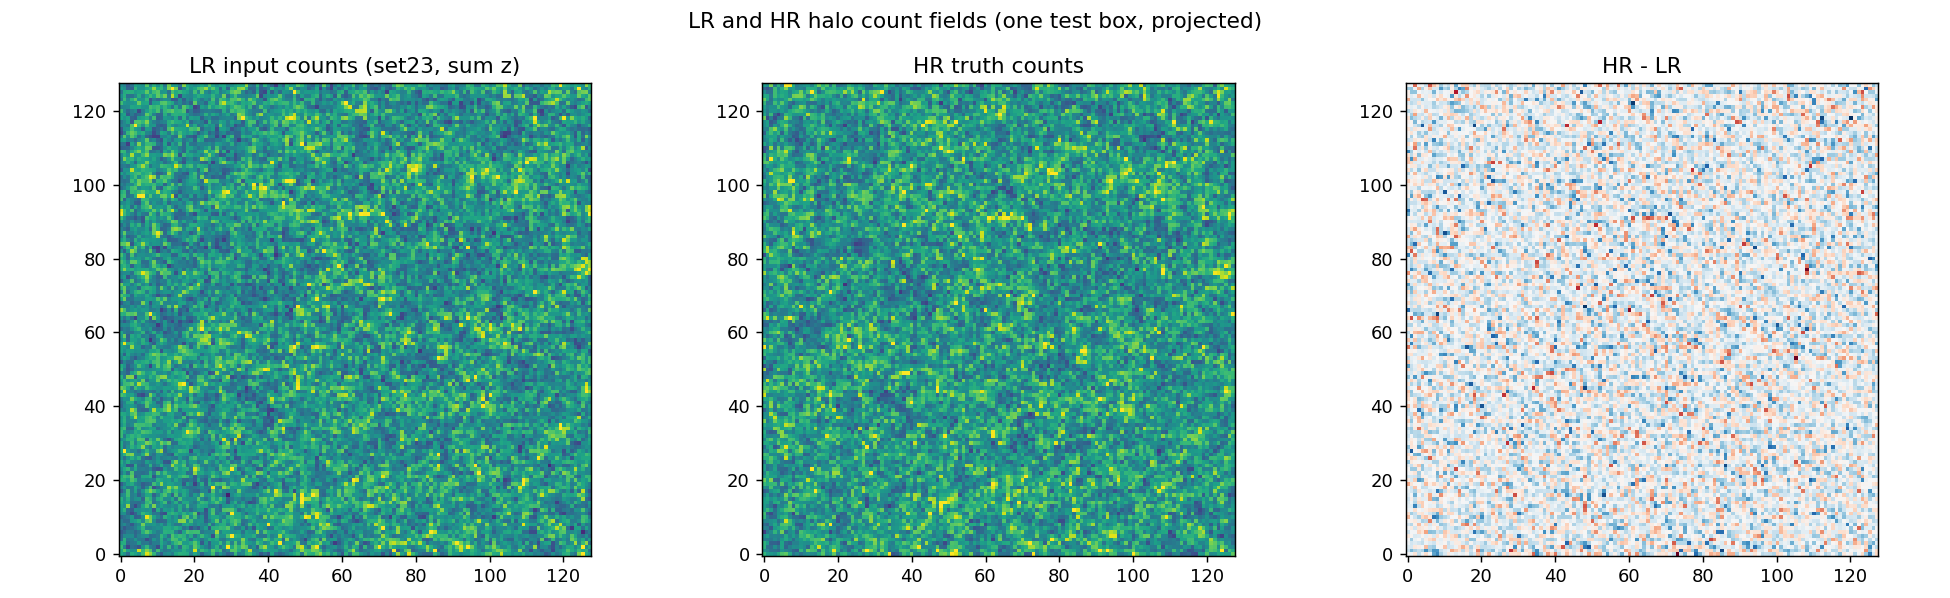
\includegraphics[width=0.9\linewidth]{figures_cmass/data_pair.png}
\caption{One LR/HR pair (projected count map). LR (FastPM, input) and HR
(Quijote N-body, target) share initial conditions and so share large-scale
structure, but differ cell-by-cell.}
\label{fig:srs-datapair}
\end{figure}

\paragraph{Model space (count transform).} The network does not learn on raw
counts; it learns in a compressed ``model space''. The default transform is
$\log(1+n)$, which tames the sparse heavy tail:
\begin{equation}
  y = \log(1+n), \qquad n = \exp(y)-1 \ \ (\text{clamped to } n\ge 0).
  \label{eq:srs-transform}
\end{equation}
Two alternative transforms exist in the code (\texttt{scale}: $n/\text{scale}$;
\texttt{delta}: model space is the overdensity itself), but all reported runs use
$\log(1+n)$. Power spectra are \emph{never} computed in model space; they are
always computed on the physical-count overdensity \SG{Is it okay if this is -1 when there are 0 halos?}
\begin{equation}
  \delta = \frac{n}{\bar n} - 1,
  \label{eq:srs-delta}
\end{equation}
with $\bar n$ the per-box mean count (the \texttt{perbox} setting used in all
runs).

\subsection{Data Pipeline (patching)}
\textit{Located in: \texttt{data/patch\_dataset\_cmass.py},
\texttt{data/patch\_dataset\_real.py} (shared patch ops).}

A model never sees the whole $128^3$ box at once. We cut the box into a
$2\times2\times2$ grid of $64^3$ \textbf{cores} (Table~\ref{tab:srs-notation}).
The cores tile the box exactly (stride $64$), so they reconstruct the box
bit-for-bit with no gaps and no double counting, the dataset's self-test
asserts this. Each model \emph{input} is a core grown by \texttt{pad} voxels on
every side, taken from the true neighbour cells with periodic wrap at the box
edge (\texttt{extract\_patch} uses \texttt{numpy.take(\dots, mode="wrap")}). So
with \texttt{pad}${=}8$ the input is $80^3$ and neighbouring patches overlap by
$2\cdot\texttt{pad}=16$ voxels; the HR \emph{target} is always the bare $64^3$
core. Because each simulation is one continuous periodic box that we crop
ourselves, the patches are real neighbours by construction, there is no data
seam (unlike the Lagrangian patches of \S5). \SG{Isn't the patch construction same in both?}

\begin{table}[t]
\centering
\caption{Notation for the CMASS count-field pipeline.}
\label{tab:srs-notation}
\begin{tabular}{llp{7.2cm}}
\toprule
Symbol & Value & Meaning \\
\midrule
$N_\text{full}$    & $128$ & full box side (voxels) \\
$P$ (\texttt{PATCH}) & $64$ & core side (voxels) \\
$N_\text{patches}$ & $8$ & cores per box ($2{\times}2{\times}2$) \\
\texttt{pad}       & $0$ (Arm A) / $8$ (Arm B) & halo width added to each face by periodic wrap \\
$L_\text{box}$     & $1000\ \mathrm{Mpc}/h$ & box side \\
$\mathbf s$        & $\in\mathbb R^5$ & cosmology vector $(\Omega_m,\Omega_b,h,n_s,\sigma_8)$ \\
$\bar n$           & per-box mean & mean count used to form $\delta=n/\bar n-1$ \\
\bottomrule
\end{tabular}
\end{table}

\begin{figure}[t]
\centering
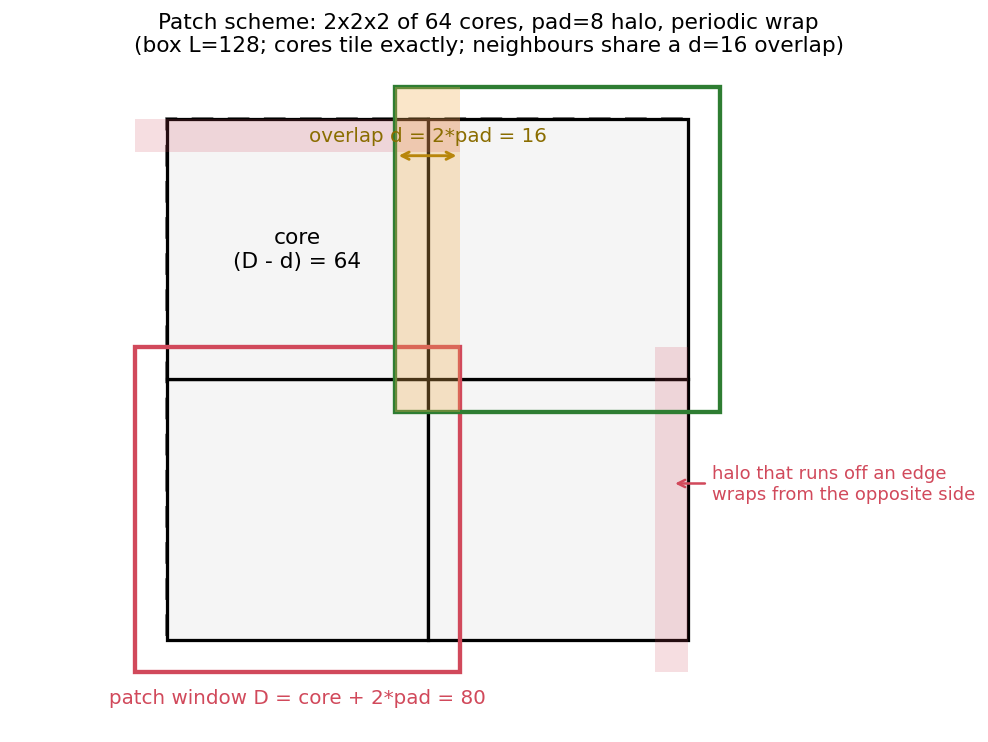
\includegraphics[width=0.82\linewidth]{figures_cmass/pipeline_patching.png}
\caption{Patch scheme. The box is cut into a $2{\times}2{\times}2$ grid of
$64^3$ cores that tile it exactly. With \texttt{pad}${>}0$ each patch is grown by
a halo of real neighbour cells (periodic wrap); only the central core is kept
and placed back.}
\label{fig:srs-patching}
\end{figure}

\paragraph{Per-simulation item.} Indexed by simulation, the dataset returns, for
all $8$ cores at once: the LR patches \texttt{lr\_in} of shape
$(8,\,1,\,64{+}2\,\texttt{pad},\,\cdot,\,\cdot)$ in model space, the HR cores
\texttt{hr\_tgt} of shape $(8,\,1,\,64,\,64,\,64)$, the style $\mathbf s$, and
the simulation index. The trainer flattens the $8$-core axis into the batch.

\begin{algorithm}[H]
\caption{\textsc{ExtractPatches} (one simulation)}
\label{alg:srs-extract}
\begin{algorithmic}[1]
\Require LR box $\mathbf L\in\mathbb R^{1\times128^3}$, HR box $\mathbf H$, \texttt{pad}
\State map $\mathbf L,\mathbf H$ to model space via Eq.~\ref{eq:srs-transform}
\For{$p=0,\dots,7$}
  \State $(i,j,k)\gets\textsc{unravel}(p,(2,2,2))$ \Comment{core origin $(64i,64j,64k)$}
  \State $\mathbf L_p\gets$ core $p$ grown by \texttt{pad} on each face, periodic wrap \Comment{$(64{+}2\,\texttt{pad})^3$}
  \State $\mathbf H_p\gets$ bare core $p$ \Comment{$64^3$}
\EndFor
\State \Return $\{(\mathbf L_p,\mathbf H_p)\}_{p=0}^{7}$, style $\mathbf s$
\end{algorithmic}
\end{algorithm}

\subsection{Model: Input/Output Specification}
\textit{Implementation: \texttt{map2map/models/styled\_srsgan.py}
(\texttt{G\_correct}, \texttt{D\_const}).}

\paragraph{What the generator computes.} The generator is a
\textbf{same-resolution residual} network: it does not change the grid size, and
it predicts a correction that is \emph{added} to the input. In model space,
\begin{equation}
  \mathrm{SR} \;=\; \mathrm{LR} \;+\; G(\mathrm{LR},\,\mathbf s,\,\mathbf z),
  \label{eq:srs-residual}
\end{equation}
where $\mathbf s$ is the cosmology vector and $\mathbf z$ is an injected noise
field (see below). Inputs and outputs are listed in
Table~\ref{tab:srs-model-io}; the generator is run once per core (the $8$ cores
of a box form a batch).

\begin{table}[t]
\centering
\caption{Tensors consumed/produced by the generator \texttt{G\_correct} for one
core (batch dimension omitted). Here $D=64{+}2\,\texttt{pad}$.}
\label{tab:srs-model-io}
\begin{tabular}{lll}
\toprule
Symbol & Shape & Meaning \\
\midrule
$\mathbf x$ (\texttt{x})       & $(1,D,D,D)$ & LR patch, model space (input) \\
$\mathbf s$ (\texttt{style})   & $(5,)$      & cosmology vector \\
$\mathbf z$ (\texttt{noise\_list}) & $2\cdot\texttt{num\_blocks}$ cubes $(1,D,D,D)$ & injected noise; fixed at inference, random in training \\
$G(\cdot)$                     & $(1,D,D,D)$ & predicted residual $\delta$ (added to $\mathbf x$) \\
\bottomrule
\end{tabular}
\end{table}

\paragraph{Internal composition.} $G$ is a constant-resolution StyleGAN2-style
network (no up/down-sampling), built from:
\begin{enumerate}
  \item \texttt{block0}: a $1{\times}1{\times}1$ style-modulated convolution
  (\texttt{ConvStyled3d}) lifting the $1$-channel input to $c_0$ channels,
  followed by a leaky ReLU.
  \item \texttt{num\_blocks} ($=4$) constant-resolution H-blocks
  (\texttt{HBlock\_const}). Each block, in order: inject noise $\to$
  $3{\times}3{\times}3$ \texttt{ConvStyled3d} (periodic ``circular'' padding)
  $\to$ leaky ReLU $\to$ inject noise $\to$ $3{\times}3{\times}3$
  \texttt{ConvStyled3d} $\to$ leaky ReLU $\to$ a $1{\times}1{\times}1$ projection
  to the output channel, accumulated into a running output $y$. The final return
  is $\mathbf x + y$ (Eq.~\ref{eq:srs-residual}).
\end{enumerate}
The channel widths come from \texttt{chan\_base} ($=128$) halved per block and
clamped to $[64,512]$. Two mechanisms make the convolutions depend on side
information:
\begin{itemize}
  \item \textbf{Style modulation.} \texttt{ConvStyled3d} is the StyleGAN2
  modulated/demodulated convolution: the cosmology vector $\mathbf s$ scales the
  convolution weights, so the same network behaves differently for different
  cosmologies. This is the only path by which $\mathbf s$ enters.
  \item \textbf{Noise injection.} Each \texttt{ConvStyled3d} is preceded by a
  per-channel learned-standard-deviation noise add (\texttt{\_NoiseInject}). At
  training time the noise is fresh Gaussian each call; at inference a
  \emph{fixed} list of noise cubes (seeded, built by \texttt{build\_noise\_list})
  is reused so outputs are reproducible. The noise is what lets the model produce
  a plausible small-scale field rather than a single blurred guess.
\end{itemize}

\paragraph{Discriminator.} \texttt{D\_const} is a constant-input-resolution
critic conditioned on the same style $\mathbf s$. It runs a head
\texttt{ConvStyled3d} then \texttt{num\_blocks} strided down-blocks (each a
periodic $3{\times}3{\times}3$ \texttt{ConvStyled3d} $+$ leaky ReLU $+$
$2{\times}$ average pool), a $1{\times}1{\times}1$ tail, and a final
$1{\times}1{\times}1$ projection to one channel, averaged over space to a single
logit per core.

\subsection{Training Step}
\textit{Located in: \texttt{train\_patch\_cmass.py}.}

The generator is trained per core (stitching is \emph{not} part of the
gradient). The total generator loss is a weighted sum of three terms,
\begin{equation}
  \mathcal L_G \;=\; \lambda_\text{adv}\,\mathcal L_\text{adv}
                  + \lambda_\text{rec}\,\mathcal L_\text{rec}
                  + \lambda_\text{pk}\,\mathcal L_\text{pk},
  \label{eq:srs-lossG}
\end{equation}
with (defaults from the original run script; see the protocol update below for
the values now in use):
\begin{itemize}
  \item \textbf{Reconstruction} $\mathcal L_\text{rec}=\lVert \mathrm{SR}-\mathrm{HR}\rVert_1$,
  a plain $L_1$ in model space (optionally Gaussian-smoothed; smoothing off in
  all runs).
  \item \textbf{Power-spectrum} $\mathcal L_\text{pk}$, the mean-squared error
  between the $\log_{10}$ power spectra of SR and HR, computed on the
  \emph{physical-count overdensity} of the $64^3$ core (Eqs.~\ref{eq:srs-transform}--\ref{eq:srs-delta}),
  Hann-windowed, with the HR side detached:
  \begin{equation}
    \mathcal L_\text{pk} = \frac{1}{|K|}\sum_{k\in K}
      \big(\log_{10} P_\text{SR}(k) - \log_{10} P_\text{HR}(k)\big)^2 .
    \label{eq:srs-pkloss}
  \end{equation}
  \item \textbf{Adversarial} $\mathcal L_\text{adv}=\mathrm{softplus}\!\big({-}D(\mathrm{SR},\mathbf s)\big)$,
  the non-saturating GAN generator loss.
\end{itemize}

\paragraph{Protocol update: what region the reconstruction and adversarial
terms see.} A \texttt{--pad-loss} setting controls how much of the generator's
output the $L_1$ and adversarial terms are computed on, independent of
\texttt{pad} itself:
\begin{itemize}
  \item \texttt{crop} (trim-aware, the setting used for Arm B above): the loss
  is computed only on \textsc{cropInterior}$(G(\mathbf x,\mathbf s),\,\texttt{pad})$,
  the $64^3$ core that is actually kept at inference time, against the bare
  $64^3$ HR core. The model is trained on exactly the region it will be graded
  on.
  \item \texttt{full}: the loss is computed on the whole $(64{+}2\,\texttt{pad})^3$
  output, against a correspondingly padded HR target (the dataset's
  \texttt{pad\_target} option). The model is trained as if the halo region it
  will later be trimmed off also mattered.
\end{itemize}
Concretely, let $\texttt{loss\_crop}=\texttt{pad}$ under \texttt{crop} and $0$
under \texttt{full}; every place above that writes $\mathrm{SR}$ means
$\textsc{cropInterior}(G(\mathbf x,\mathbf s),\,\texttt{loss\_crop})$, and the
Hann window and $P(k)$ estimator in $\mathcal L_\text{pk}$ are sized to match.
This is a controlled test of two ways padding could fail to help: see the
protocol-update subsection below for the result.

The discriminator is trained with the non-saturating GAN loss plus a lazy $R_1$
gradient penalty applied every \texttt{r1\_every} steps:
\begin{equation}
  \mathcal L_D = \mathrm{softplus}\!\big({-}D(\mathrm{HR})\big)
               + \mathrm{softplus}\!\big(D(\mathrm{SR})\big)
               + \tfrac{1}{2}\lambda_{R_1}\,\mathbb E\big\lVert \nabla_{\!x} D(x,\mathbf s)\big\rVert^2 .
  \label{eq:srs-lossD}
\end{equation}

\begin{algorithm}[H]
\caption{CMASS patch-GAN training step (one batch of cores)}
\label{alg:srs-train}
\begin{algorithmic}[1]
\Require LR patches $\mathbf x$, HR targets $\mathbf h$ (padded iff \texttt{pad-loss=full}),
         style $\mathbf s$, \texttt{pad}, \texttt{loss\_crop} ($=\texttt{pad}$ if \texttt{crop} else $0$),
         weights $\lambda_\text{adv},\lambda_\text{rec},\lambda_\text{pk},\lambda_{R_1}$
\Statex \textbf{// Discriminator}
\State $\hat{\mathbf h}\gets \textsc{cropInterior}\big(G(\mathbf x,\mathbf s),\,\texttt{loss\_crop}\big)$ \Comment{no grad}
\State $\mathcal L_D \gets \mathrm{softplus}({-}D(\mathbf h,\mathbf s)) + \mathrm{softplus}(D(\hat{\mathbf h},\mathbf s))$
\If{step $\bmod\ \texttt{r1\_every} = 0$} $\mathcal L_D \mathrel{+}= \tfrac12\lambda_{R_1}\texttt{r1\_every}\cdot R_1(D,\mathbf h,\mathbf s)$ \EndIf
\State update $D$ (Adam, grad-clip)
\Statex \textbf{// Generator}
\State $\hat{\mathbf h}\gets \textsc{cropInterior}\big(G(\mathbf x,\mathbf s),\,\texttt{loss\_crop}\big)$
\State $\mathcal L_\text{adv}\gets \mathrm{softplus}({-}D(\hat{\mathbf h},\mathbf s))$
\State $\mathcal L_\text{rec}\gets \lVert \hat{\mathbf h}-\mathbf h\rVert_1$
\State $\mathcal L_\text{pk}\gets$ Eq.~\ref{eq:srs-pkloss} on Hann-windowed overdensity of $\hat{\mathbf h}$, $\mathbf h$
       (skip if $\lambda_\text{pk}{=}0$)
\State $\mathcal L_G \gets \lambda_\text{adv}\mathcal L_\text{adv}+\lambda_\text{rec}\mathcal L_\text{rec}+\lambda_\text{pk}\mathcal L_\text{pk}$
\State update $G$ (Adam, grad-clip)
\end{algorithmic}
\end{algorithm}

\paragraph{Validation and checkpoint selection.} After each epoch we stitch the
full $128^3$ SR box for up to $40$ validation sims and report the stitched
$L_1$/voxel and the stitched-$128$ power-spectrum RMS against HR
(\S\ref{sec:srs-eval}, Eq.~\ref{eq:srs-pkrms}). A \texttt{--select} setting
chooses which of the two the saved \texttt{best.pt} tracks: \texttt{pk} (the
original setting, lowest stitched validation Pk RMS) or \texttt{l1} (lowest
stitched validation $L_1$/voxel). Selection is always on the stitched full box,
not the per-core training loss. Runs that also train with $\lambda_\text{pk}{=}0$
use \texttt{--select l1}, since selecting on Pk RMS while not training on it
would reintroduce the same metric leak in a different place.

\subsection{Inference}
\textit{Located in: \texttt{infer\_stitch\_cmass.py}.}

For one simulation: load the LR $128^3$ count box, map it to model space, run $G$
on each of the $8$ cores (with the periodic-wrap halo in Arm B), crop the halo,
stitch the cores into a $128^3$ model-space box, invert the transform to physical
counts, and clamp. \SG{are all outputs later mapped to integers, or are we fine with non-integer number of halos?} The injected noise list is fixed (seeded) so the output is
reproducible.

\begin{algorithm}[H]
\caption{CMASS inference + stitch (one simulation)}
\label{alg:srs-infer}
\begin{algorithmic}[1]
\Require LR box $\mathbf L$, style $\mathbf s$, trained $G$, mode (naive/overlap), fixed noise $\mathbf z$
\State $\texttt{pad}\gets 0$ if naive else value from checkpoint ($8$)
\State map $\mathbf L$ to model space (Eq.~\ref{eq:srs-transform})
\For{$p=0,\dots,7$}
  \State $\mathbf x_p\gets$ patch $p$ (core grown by \texttt{pad}, periodic wrap)
  \State $\mathbf c_p\gets \textsc{cropInterior}\big(G(\mathbf x_p,\mathbf s,\mathbf z),\,\texttt{pad}\big)$ \Comment{$64^3$ core, model space}
\EndFor
\State $\mathbf S\gets \textsc{stitch}(\{\mathbf c_p\})$ \Comment{$128^3$, model space}
\State $\mathbf S\gets \exp(\mathbf S)-1$, clamp to $[0,\,C_\text{max}{=}200]$, replace NaN/Inf \Comment{physical counts}
\State \Return $\mathbf S$
\end{algorithmic}
\end{algorithm}

\subsection{Crop Stitching}

Stitching is \textbf{direct placement with no averaging}. Adjacent cores tile the
box exactly (stride $64$, no overlap between cores once the halo is dropped), so
each core's $64^3$ output is written straight into its slot. In Arm B the $80^3$
patch is corrected and only its central $64^3$ core is kept; the overlap halo is
context for the convolution, never written to the output.

\begin{algorithm}[H]
\caption{\textsc{Stitch} ($8$ cores $\to$ $128^3$)}
\label{alg:srs-stitch}
\begin{algorithmic}[1]
\Require cores $\{\mathbf c_p\}_{p=0}^{7}$, each $1\times64^3$
\State $\mathbf S\gets \mathbf 0\in\mathbb R^{1\times128^3}$
\For{$p=0,\dots,7$}
  \State $(i,j,k)\gets\textsc{unravel}(p,(2,2,2))$
  \State $\mathbf S[:,\,64i{:}64i{+}64,\,64j{:}\cdots,\,64k{:}\cdots]\gets \mathbf c_p$ \Comment{direct assignment}
\EndFor
\State \Return $\mathbf S$
\end{algorithmic}
\end{algorithm}

\subsection{Evaluation}
\label{sec:srs-eval}
\textit{Located in: \texttt{analysis/eval\_seam\_cmass.py},
\texttt{analysis/diag\_cmass.py}, \texttt{analysis/match\_stats\_cmass.py},
\texttt{analysis/power\_spectrum.py}, \texttt{inference/nde.py},
\texttt{evaluate.py}.}

We evaluate the SR field against HR at three levels: a seam check (does stitching
leave a join?), field statistics (does SR have the right structure?), and
cosmology (does SR give the same parameter posterior as HR?).

\paragraph{Power-spectrum summaries.} On the count overdensity (Eq.~\ref{eq:srs-delta})
we report the power spectrum $P(k)$, the transfer ratio, and the cross-coherence:
\begin{equation}
  T(k) = \frac{P_\text{SR}(k)}{P_\text{HR}(k)},
  \qquad
  r(k) = \frac{P_{\text{SR},\text{HR}}(k)}{\sqrt{P_\text{SR}(k)\,P_\text{HR}(k)}} .
  \label{eq:srs-Tr}
\end{equation}
$T(k)=1$ means SR has the right \emph{amount} of power at scale $k$ (amplitude);
$r(k)=1$ means SR has the structure in the right \emph{place} (phase). The
scalar power-spectrum error used for checkpoint selection and seam reporting is
the log-RMS over the resolved $k$-bins:
\begin{equation}
  \mathrm{PkRMS}_{\log_{10}} = \sqrt{\frac{1}{|K|}\sum_{k\in K}
    \big(\log_{10} P_\text{SR}(k) - \log_{10} P_\text{HR}(k)\big)^2 } .
  \label{eq:srs-pkrms}
\end{equation}

\paragraph{Seam diagnostic.} \texttt{eval\_seam\_cmass.py} bins the per-cell
count error $|{\mathrm{SR}-\mathrm{HR}}|$ by distance to the nearest core face
and forms a per-position error profile along each axis. The headline number is
the \textbf{$x{=}64$ internal-seam excess}: the error on the internal core
boundary plane divided by the interior error. A value near $1$ means stitching
leaves no seam. The box edge $x{=}0$ is a periodic-boundary control.

\paragraph{Field-match statistics.} \texttt{match\_stats\_cmass.py} reports, over
$16$ test boxes: the total-count ratio $\sum\mathrm{SR}/\sum\mathrm{HR}$, the
void fraction (cells $<0.5$), the real-space cell standard-deviation ratio
$\mathrm{std}(\mathrm{SR})/\mathrm{std}(\mathrm{HR})$ (a blur check), and the
cross-coherence $r(k)$ at large ($k<0.05$) and small ($k>0.2$) scales.

\paragraph{Cosmology (posterior consistency).} This is the strongest ``does SR
match HR'' test. We voxel-count $\to$ overdensity $\to$ $P(k)$ for every box, then
train a neural density estimator $q(\theta\mid P(k))$ on the training split using
\texttt{sbi} (\texttt{SNPE\_C} with a neural-spline-flow density estimator,
\texttt{inference/nde.py}); the summary is $\log_{10}P(k)$. We train one estimator
on HR ($q_\text{HR}$) and one on each SR arm ($q_\text{SR}$). For each test box we
draw $2000$ posterior samples from each, fit a Gaussian per parameter, and report
the per-parameter Gaussian KL (\texttt{evaluate.py}):
\begin{equation}
  \mathrm{KL}\big(\mathcal N(\mu_\text{HR},\sigma_\text{HR})\,\Vert\,\mathcal N(\mu_\text{SR},\sigma_\text{SR})\big)
  = \tfrac12\!\left[\log\frac{\sigma_\text{SR}^2}{\sigma_\text{HR}^2}
    + \frac{\sigma_\text{HR}^2+(\mu_\text{HR}-\mu_\text{SR})^2}{\sigma_\text{SR}^2} - 1\right].
  \label{eq:srs-kl}
\end{equation}
$\mathrm{KL}=0$ means SR gives the identical cosmology posterior to HR. The raw LR
field (no model), pushed through the same pipeline, is the control SR must beat.

We report this comparison in two forms, and it matters which is which:
\begin{itemize}
  \item \textbf{Cross-fidelity (primary).} $q_\text{SR}$ is trained on SR power
  spectra but \emph{evaluated on the HR} $P(k)$ of each test simulation, and
  compared to $q_\text{HR}$ evaluated on the same HR $P(k)$. This is the
  deployment scenario the project targets: HR simulations are too expensive to
  train an inference model on, so the inference model is trained on cheap SR
  output and must still work when applied to (HR-like) reality. The comparison
  against an LR-trained estimator on the same HR data measures whether sampling
  in HR space (SR) survives the distribution shift better than staying in LR
  space. This metric never appears in the training loss.
  \item \textbf{Own-data (secondary).} $q_\text{SR}$ trained and evaluated on SR
  vs $q_\text{HR}$ trained and evaluated on HR, each pipeline end-to-end on
  its own field type.
\end{itemize}

\subsection{Best-Run Configuration}
\textit{Run script: \texttt{scripts/train\_patch\_cmass.slurm}; checkpoints
\texttt{checkpoints/patch\_cmass\_\{A,B\}/best.pt}.}

Both arms use the identical configuration below; they differ only in \texttt{pad}
($0$ for Arm~A, $8$ for Arm~B). This is the configuration behind every number
in \S\ref{sec:srs-results}--\S\ref{sec:srs-next}.

\begin{lstlisting}[language=bash]
--transform log1p   --nbar perbox        # log(1+n) model space; per-box nbar
--epochs 30         --sims-per-batch 1    # patch-batch = 8 cores per step
--chan-base-g 128   --chan-base-d 64  --num-blocks 4
--lambda-adv 1.0    --lambda-rec 2.0  --lambda-pk 2.0   # generator weights
--lambda-r1 10.0    --r1-every 16                       # lazy R1
--lr-g 1e-4 --lr-d 1e-4  --beta1 0.0 --beta2 0.99       # Adam
--grad-clip 1.0     --val-max-sims 40    --select pk    # select on Pk RMS
\end{lstlisting}

The best checkpoint per arm is the one with the lowest stitched validation Pk RMS
(Eq.~\ref{eq:srs-pkrms}):

\begin{center}
\begin{tabular}{lc}
\toprule
arm & best stitched val PkRMS$_{\log_{10}}$ \\
\midrule
Arm A, naive (pad $0$)  & $0.0947$ \\
Arm B, overlap (pad $8$) & $0.0963$ \\
\bottomrule
\end{tabular}
\end{center}

\paragraph{Protocol update.} Following the mentor meeting reported in
\S\ref{sec:srs-followup}, the configuration above is no longer the one we train
with. Three settings changed:
\begin{lstlisting}[language=bash]
--lambda-pk 0.0      # power-spectrum term OFF (it was also our main metric)
--pad-loss crop|full # trim-aware vs trim-unaware padding, see below
--select l1          # select on stitched L1, not the term we removed
\end{lstlisting}
All results in \S\ref{sec:srs-followup} use this configuration. Runs under the
original configuration above (Arm A, Arm B, and everything derived from them in
\S\ref{sec:srs-results}--\S\ref{sec:srs-next}) remain valid as a record of that
protocol; they are superseded, not invalidated, by the update.

\subsection{Results: Does SR Match HR?}
\label{sec:srs-results}

All numbers are on the $200$-box test split unless noted.

\paragraph{1. Power spectrum (statistics).} Across the test set the SR power
spectrum tracks HR at every scale, and Arm A beats the no-model LR control on the
overall log-RMS (Fig.~\ref{fig:srs-srvshr}, computed by
\texttt{analysis/plot\_sr\_vs\_hr.py}).

\begin{table}[h]
\centering
\caption{SR vs HR power-spectrum agreement, $200$ test boxes. Transfer
$T(k)=P_X/P_\text{HR}$ (Eq.~\ref{eq:srs-Tr}); $1.0$ is perfect.}
\label{tab:srs-pk}
\begin{tabular}{lccc}
\toprule
field (vs HR) & PkRMS$_{\log_{10}}$ & $T$ at large scales ($k{<}0.1$) & $T$ at small scales ($k{>}0.3$) \\
\midrule
SR (Arm A, naive)    & $\mathbf{0.0607}$ & $0.95$ & $1.04$ \\
SR (Arm B, overlap)  & $0.0645$ & $0.93$ & $0.88$ \\
LR (no model, control) & $0.0641$ & $1.01$ & $1.01$ \\
\bottomrule
\end{tabular}
\end{table}

\begin{figure}[t]
\centering
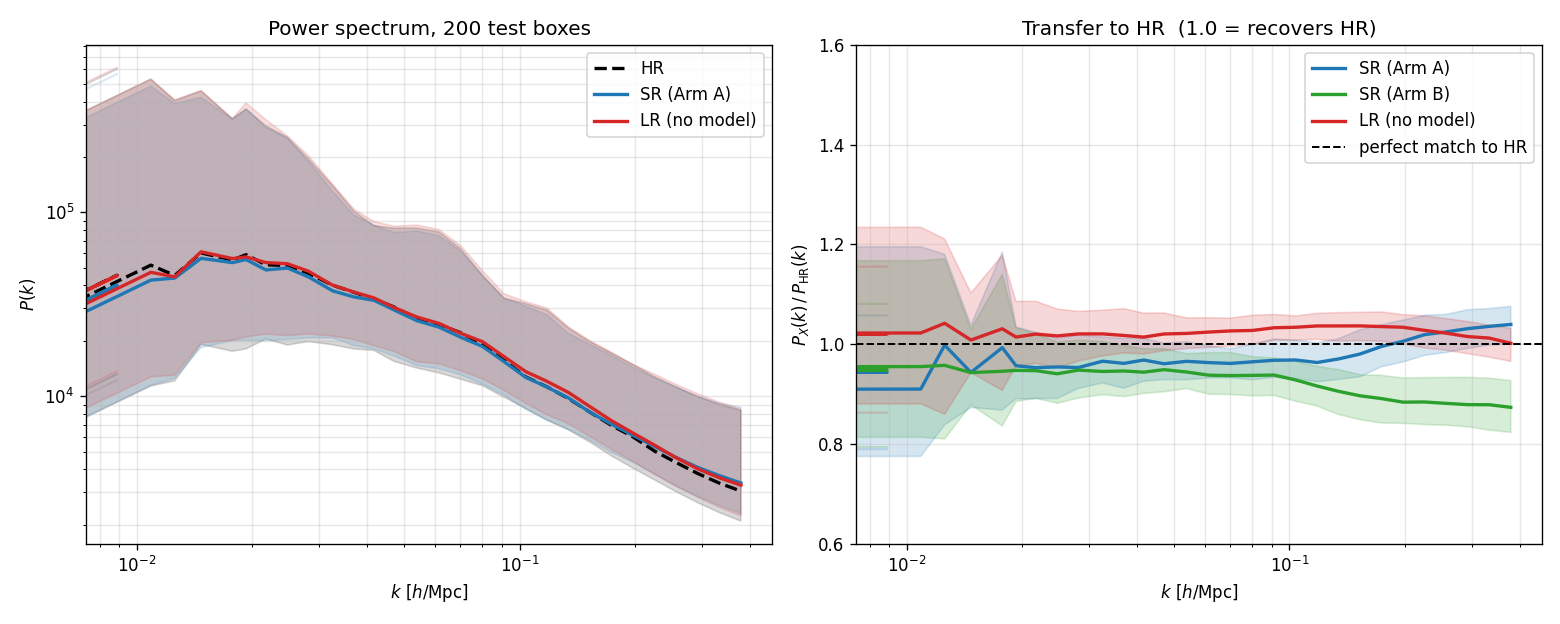
\includegraphics[width=0.98\linewidth]{figures_cmass/sr_vs_hr_pk.png}
\caption{\textbf{Left:} $P(k)$ of HR, SR (Arm A), and LR over $200$ test boxes
(median $+$ $16/84\%$ band). \textbf{Right:} transfer to HR; $1.0$ recovers HR.
SR (Arm A) sits near $1$ at all scales; Arm B's overlap blending slightly
suppresses small-scale power (transfer $0.88$).}
\label{fig:srs-srvshr}
\end{figure}

\paragraph{2. Field structure.} Beyond the power spectrum, SR keeps the field
structure of HR (Arm A, $16$ test boxes, \texttt{match\_stats\_cmassA.txt}):

\begin{table}[h]
\centering
\caption{SR vs HR field-match statistics (Arm A).}
\label{tab:srs-match}
\begin{tabular}{lll}
\toprule
quantity & value & reading \\
\midrule
total count ratio $\sum\mathrm{SR}/\sum\mathrm{HR}$ & $0.965\pm0.172$ & counts conserved on average; large per-box scatter \\
real-space std ratio & $1.008\pm0.100$ & clustering amplitude matches; not blurred \\
void fraction SR / HR ($<0.5$) & $0.855$ / $0.833$ & SR keeps voids empty, like HR \\
cross-coherence $r$, $k<0.05$ & $0.951$ & large-scale structure matches cell-by-cell \\
cross-coherence $r$, $k>0.2$ & $0.403$ & small-scale structure decorrelates \\
\bottomrule
\end{tabular}
\end{table}

\paragraph{3. Cosmology.} The cosmology comparison in the original report used
mislabeled cosmologies, an indexing bug we describe and fix in
\S\ref{sec:srs-correction}, so those numbers are not shown here. With correct
labels a single box constrains $\Omega_m$ and $\sigma_8$; at the power spectrum
level the raw LR field is already HR-like, while at the field level an SR-trained
posterior transfers to HR and an LR-trained one does not
(\S\ref{sec:srs-correction}, Table~\ref{tab:srs-corrected}).

\paragraph{4. Seam.} Neither arm introduces a stitching seam: the $x{=}64$
internal-seam excess is $\approx1$ for both
(Table~\ref{tab:srs-seam}, Fig.~\ref{fig:srs-seam}). Arm A shows a mild generic
ripple near \emph{any} boundary plane (seam-distance ratio $1.17$); Arm B's
overlap removes it ($1.00$) at a small cost in Pk RMS.

\begin{table}[h]
\centering
\caption{Seam and stitched-fidelity metrics, $200$ test boxes. ``Excess'' is
boundary error over interior error; $\approx1$ means no seam.}
\label{tab:srs-seam}
\begin{tabular}{lccp{5.2cm}}
\toprule
metric & Arm A naive & Arm B overlap & reading \\
\midrule
$x{=}64$ internal-seam excess & $0.9934$ & $0.9998$ & no internal seam either arm \\
seam-distance ratio ($d{=}0/d{\ge}8$) & $1.1729$ & $1.0032$ & generic boundary ripple, removed by overlap \\
$x{=}0$ periodic edge (control) & $0.9930$ & $0.9993$ & box edge behaves like interior \\
stitched PkRMS$_{\log_{10}}$ vs HR & $0.0637$ & $0.0678$ & stitched power-spectrum match \\
\bottomrule
\end{tabular}
\end{table}

\begin{figure}[t]
\centering
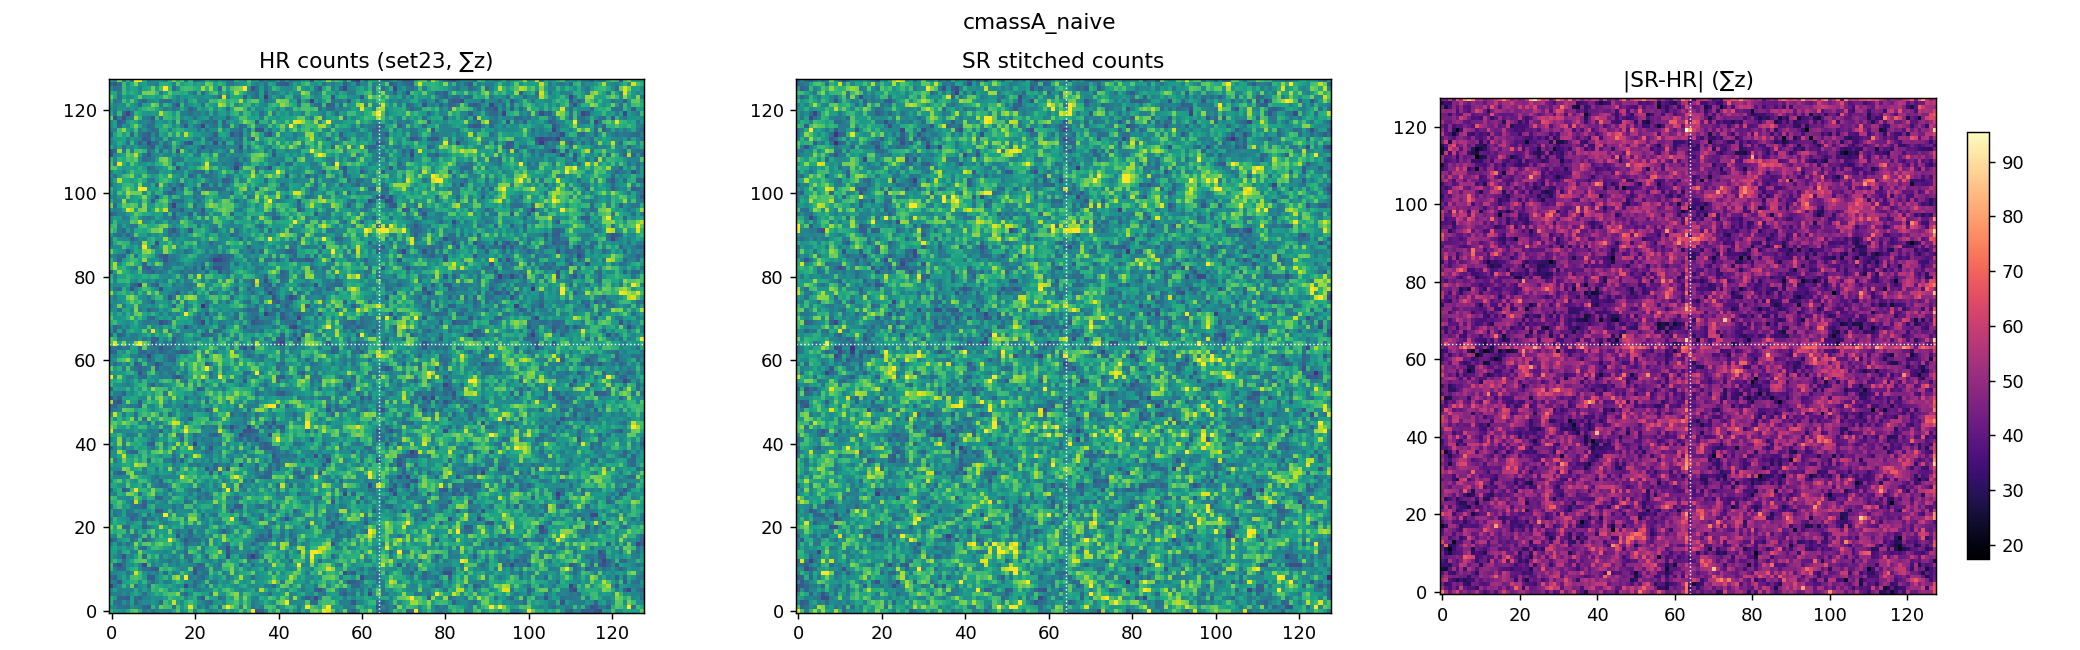
\includegraphics[width=0.95\linewidth]{figures_cmass/seam_cmassA_naive_slice.png}
\caption{Projected count maps for one test box (Arm A): HR, stitched SR, and the
absolute residual $|\mathrm{SR}-\mathrm{HR}|$. White dotted lines mark the
$x{=}64$, $y{=}64$ core boundaries; the residual shows no elevated ridge along
them.}
\label{fig:srs-seam}
\end{figure}

\paragraph{Per-scale diagnostic panels.} Figure~\ref{fig:srs-pkpanel} shows the
full-box $P(k)$, transfer, and cross-coherence for Arm A. The transfer sits near
$1$ at all scales (right amount of power); the cross-coherence is near $1$ at
large scales and falls toward small scales (structure placement is recovered at
large scales only). The per-patch panel
(\texttt{figures\_cmass/pk\_panel\_patch\_cmassAfix.png}) and the projection panels
(\texttt{projection\_box\_cmassAfix\_set23.png},
\texttt{projection\_patch\_cmassAfix\_set23\_p0.png}) tell the same story; Arm~B's
panels carry the \texttt{cmassB} suffix.

\begin{figure}[t]
\centering
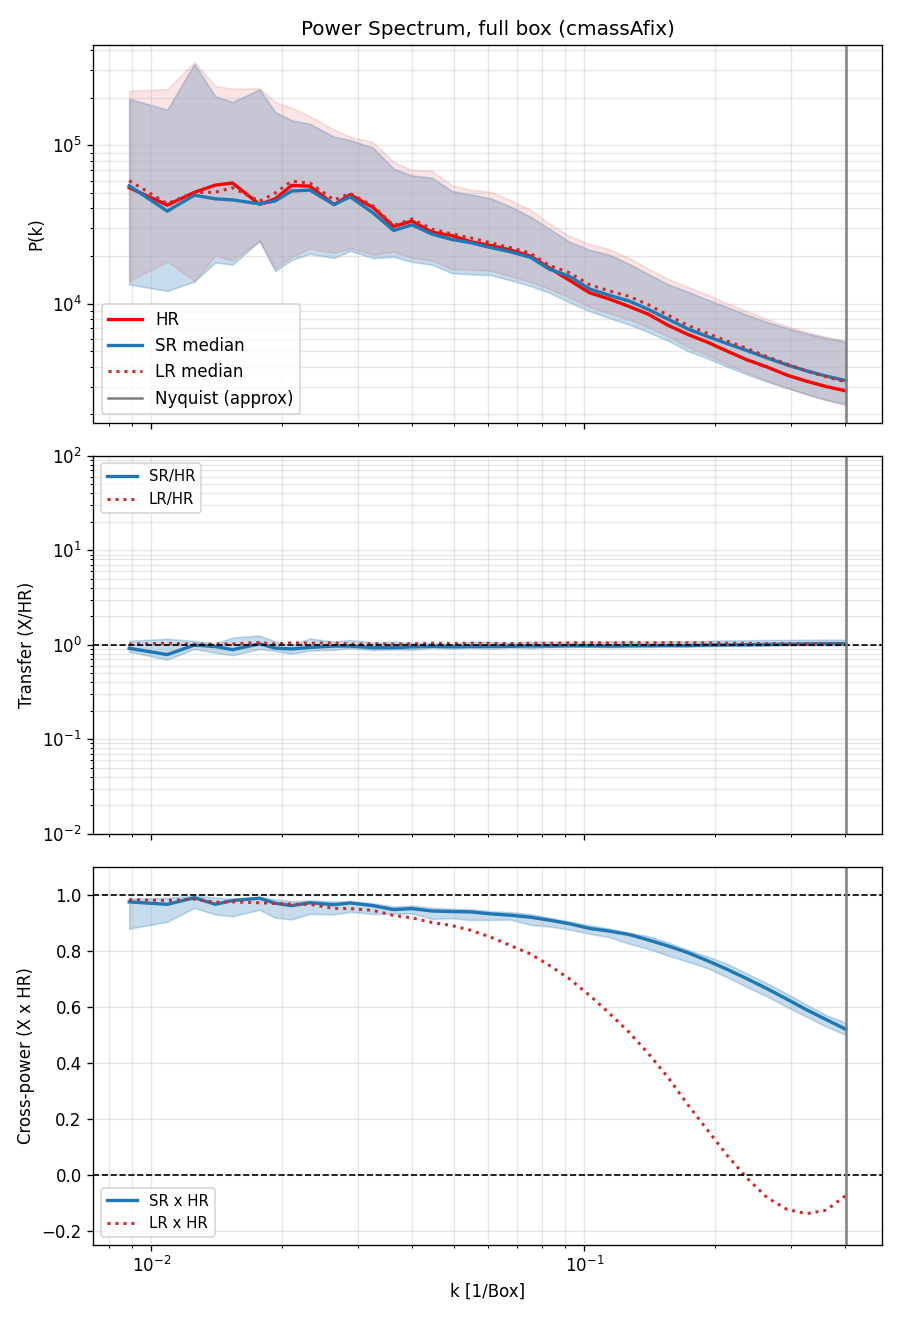
\includegraphics[width=0.5\linewidth]{figures_cmass/pk_panel_box_cmassAfix.png}
\caption{Full-box diagnostic for the conditioned generator (fiducial cosmology,
$16$ test boxes): $P(k)$ of HR (red), SR (blue median $+$ band), and LR (dotted
red); transfer $T(k)=P_X/P_\text{HR}$ on a linear axis with the 16 to 84
percentile band for both SR and LR, the legend reporting the RMS deviation of
each ratio from unity; and cross-coherence $r(k)$. The SR median transfer sits
below unity for $k<0.1$, a systematic large-scale power deficit of roughly 5 to
10 percent, while LR sits slightly above unity; SR does not tighten the transfer
scatter relative to LR. In $r(k)$, SR stays near unity to smaller scales while
LR decorrelates.}
\label{fig:srs-pkpanel}
\end{figure}

\subsection{Diagnostic: What is NOT Working}

\paragraph{Small-scale structure decorrelates, and this is fundamental.} SR
matches HR cell-by-cell at large scales ($r{=}0.95$ for $k<0.05$) but loses the
match at small scales ($r{=}0.40$ for $k>0.2$, Table~\ref{tab:srs-match}). This
is not a capacity bug: it is set by how much information the LR input carries
about HR. LR and HR share large-scale modes but the voxel-by-voxel LR$\leftrightarrow$HR
correlation is only $\approx0.06$, so the exact small-scale realization is simply
not present in the input. The model can match the small-scale \emph{statistics}
(transfer $\approx1$, real-space std ratio $1.008$) but cannot reproduce the
exact placement of individual halos. The noise injection
(Eq.~\ref{eq:srs-residual}) exists precisely because of this: it draws a
plausible small-scale field rather than regressing to a blur.

\paragraph{Per-box total-count scatter.} The total halo count is conserved on
average but with $\sim17\%$ per-box scatter ($\sum\mathrm{SR}/\sum\mathrm{HR}=
0.965\pm0.172$). A count-aware output head (predict a rate and sample Poisson
counts) would tighten this; it is the one clearly addressable imperfection. \SG{I would think this isn't necessary to fix, we don't care about the number of halos after all.}

\paragraph{Overlap suppresses small-scale power.} Arm B's overlap blending lowers
the small-scale transfer to $0.88$ (Table~\ref{tab:srs-pk}), so on the power
spectrum the naive Arm A is the better super-resolver. Overlap removes a small
generic boundary ripple but buys no fidelity, because on this continuous count
data there is no real seam to fix, the clean version of the mentor 2.1 vs 2.2
comparison.

\paragraph{Where the cosmology value is.} At the power spectrum level the raw LR
field is already close to HR, since they share large-scale modes, so the power
spectrum is a forgiving summary with little headroom. The model's value is at the
field level (variance, voids, small-scale structure), which the power spectrum
summary is insensitive to. The corrected cross-fidelity in
\S\ref{sec:srs-correction} bears this out: SR and LR are indistinguishable at the
power spectrum level, but at the field level an SR-trained posterior transfers to
HR while an LR-trained one does not.

\subsection{What I'm Trying Next}
\label{sec:srs-next}

The diagnostics above point to one limit that may be fundamental (small-scale
decorrelation) and a few that are clearly fixable (count scatter, small-scale
realism). The plan below is ordered so that we \emph{measure} the limit before
spending effort trying to beat it. None of these results are in yet; this is the
roadmap, not an experiment log.

\paragraph{Step 0, measure the information ceiling first.} Before trying to
improve the small-scale match, we need to know whether $r{=}0.40$ at small scales
(Table~\ref{tab:srs-match}) is the best any model could do from this input, or a
weakness of the current one. Two cheap diagnostics settle it:
\begin{itemize}
  \item \textbf{LR$\leftrightarrow$HR cross-coherence $r_\text{LR,HR}(k)$.} The
  cross-coherence of the \emph{raw input} against HR (no model) is the ceiling:
  no function of LR can place small-scale structure better than the input
  already correlates with HR. If $r_\text{SR,HR}(k)\approx r_\text{LR,HR}(k)$ at
  small $k$, the model is already at the ceiling and the limit is fundamental;
  if it sits well below, there is recoverable structure left on the table. (Only
  per-box $P(k)$ is currently saved, not the cross-spectrum, so this needs one
  re-run that keeps the fields.)
  \item \textbf{No-noise ablation.} Train the same generator with the noise
  injection off (a plain regressor). Theory predicts this should \emph{raise} the
  small-scale cross-coherence a little (a regressor targets the conditional mean,
  the best cell-by-cell predictor) but \emph{lower} the small-scale transfer well
  below $1$ (the conditional mean is blurry). Seeing exactly that trade-off would
  confirm that the noise/GAN is the right choice for a power-spectrum target, and
  would quantify how much cell-by-cell accuracy is being traded for correct
  statistics.
\end{itemize}

\paragraph{Step 1, fix the count scatter and small-scale realism (independent
of the ceiling).} These help regardless of what Step 0 finds:
\begin{itemize}
  \item \textbf{Count-aware (Poisson) output head.} Instead of predicting a
  count directly, predict a non-negative rate $\lambda$ per cell and sample the
  count as $n\sim\mathrm{Poisson}(\lambda)$. Halo counts are discrete and sparse,
  so a Poisson head models the small-scale graininess as actual shot noise rather
  than a smeared residual, and should tighten the $\sim17\%$ per-box total-count
  scatter (Table~\ref{tab:srs-match}), the one clearly addressable imperfection.
  \item \textbf{Explicit statistics terms in the loss.} Add a one-point PDF /
  variance matching term so small-scale sharpness is enforced directly, rather
  than relying on the adversarial term alone to find it.
  \item \textbf{Loss rebalance.} The current weights are $\lambda_\text{rec}{=}2$,
  $\lambda_\text{pk}{=}2$, $\lambda_\text{adv}{=}1$
  (Eq.~\ref{eq:srs-lossG}). The $L_1$ term blurs; lowering it and raising the
  adversarial weight should push toward correct statistics, at a known cost in
  cell-by-cell accuracy, per the same trade-off as the no-noise ablation.
\end{itemize}

\paragraph{Step 2, extract more of the available information (only if Step 0
shows headroom).} If $r_\text{SR,HR}$ sits below the LR$\leftrightarrow$HR
ceiling, the model is under-using its input. A larger receptive field, or feeding
each patch more neighbour context, would let it use more of the LR field to
predict the residual. This only helps if there is headroom to recover.

\paragraph{Step 3, raise the ceiling by changing the \emph{input}, not the
model.} The small-scale cell-by-cell limit is set by the information in the LR
input (the voxel-by-voxel LR$\leftrightarrow$HR correlation is only
$\approx0.06$). No amount of model capacity raises that; only more informative
inputs do. Candidates: feed the shared small-scale \emph{initial conditions}
(which the coarse LR count field has discarded), or add the LR velocity / particle
fields. This is the only route to a meaningful gain in small-scale cross-coherence,
and is the natural bridge to the displacement-field model of \S5, which already
carries that extra information.

\paragraph{Summary.} Steps 0--1 are the near-term plan: measure the ceiling, then
add a Poisson head and statistics losses to fix the count scatter and sharpen the
small-scale field. Steps 2--3 are contingent on what Step 0 reveals. For a
cosmology deliverable the priority is statistical fidelity (which Steps 0--1
target); exact small-scale reconstruction (Step 3) is a larger, input-level
change worth it only if cell-by-cell recovery becomes the goal.

\subsection{Follow-Up Results: New Protocol from the Mentor Meeting}
\label{sec:srs-followup}

A mentor meeting after the report above changed two things about how we train
and evaluate this model. First, the real goal is not to match HR with SR by
itself. The real goal is to train a posterior model on SR output and have it
work well when it is tested on real HR data, since HR simulations are too
expensive to train a posterior model on directly. Second, the power spectrum
term was removed from the training loss, since it was also our main success
metric and that is a weak test. This subsection reports what we found. Some of
the training runs below are still in progress at the time of writing, so
numbers marked as current are read from the latest completed epoch, not a
final result.

\paragraph{Held-out check: the bispectrum.} A fair worry is that our power
spectrum result looks good only because the power spectrum was also in the
training loss. To check this we measured the bispectrum, a higher-order
statistic that was never used anywhere in training or model selection. If SR
only matches the power spectrum and nothing else, the bispectrum should show
no improvement over the raw LR input.

\begin{figure}[t]
\centering
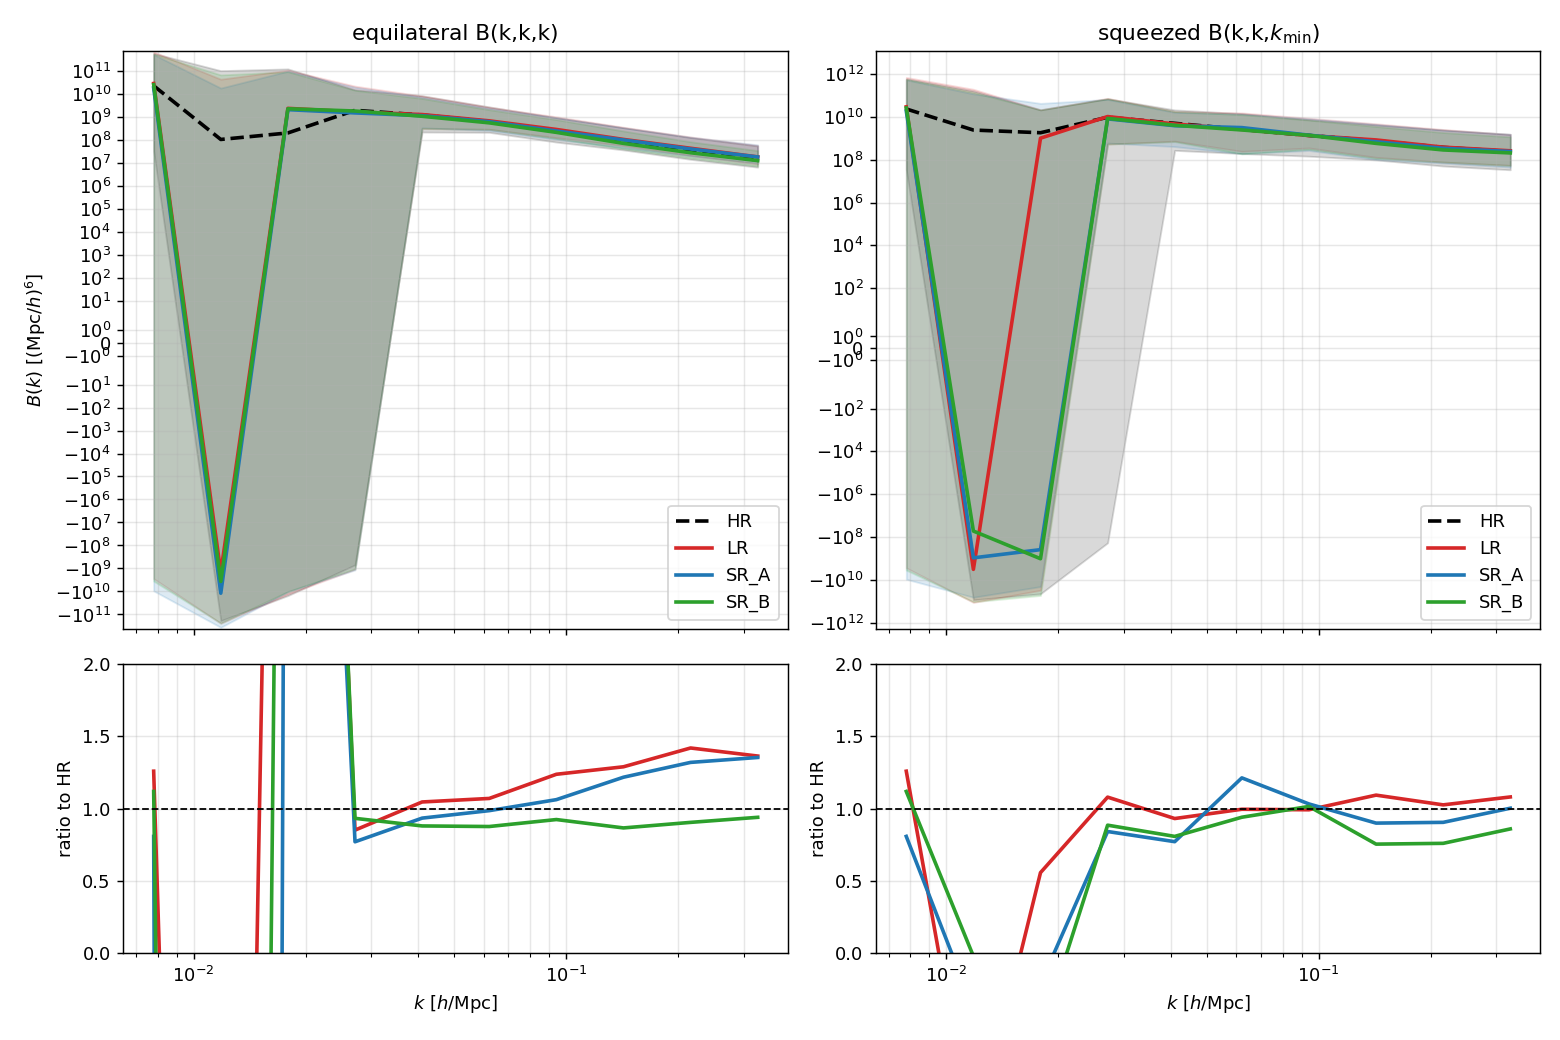
\includegraphics[width=0.95\linewidth]{figures_cmass/bispectrum_hr_lr_srA_srB.png}
\caption{Bispectrum of HR, LR, and SR (both arms), on $16$ test boxes. Top:
equilateral and squeezed bispectrum, HR in black. Bottom: ratio to HR. SR
removes most of the systematic excess that LR has at the plotted scales,
without ever training on this statistic.}
\label{fig:srs-bispec}
\end{figure}

On the equilateral configuration, LR sits about $6$ to $13$ percent above HR
across the middle range of scales. SR removes most of this gap without ever
seeing a bispectrum during training, and it does this for both arms. This is
evidence that the model is not simply fitting the training metric. It is
correcting real structure in the field that also shows up in a statistic it
never saw. (The figure uses the earlier models trained \emph{with} the power
spectrum loss; the no-Pk models of the following paragraphs preserve the
bispectrum at least as well, so removing that loss did not degrade this
held-out statistic either.)

\paragraph{Removing the power spectrum loss.} Following the meeting, we
retrained the model with the power spectrum term switched off
($\lambda_\text{pk}{=}0$ in Eq.~\ref{eq:srs-lossG}), so the loss is only the
adversarial and $L_1$ terms. We also changed which checkpoint counts as "best"
to the real-space $L_1$ error, since selecting on the power spectrum would
have been the same kind of leak we were trying to remove.

\begin{figure}[t]
\centering
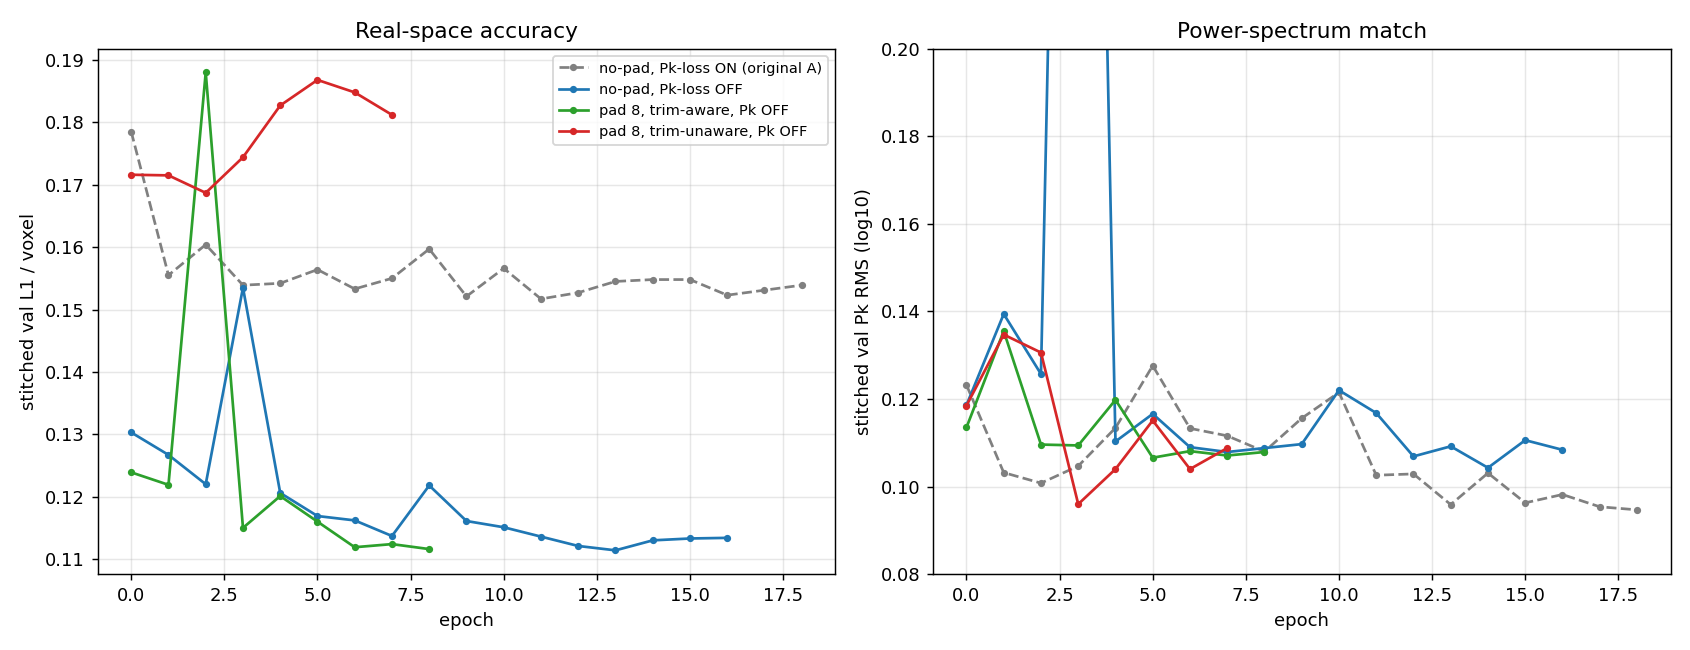
\includegraphics[width=0.98\linewidth]{figures_cmass/protocolv2_cmass.png}
\caption{Stitched validation curves under the new protocol (power spectrum
loss off). Left: real-space $L_1$ error. Right: power spectrum RMS error. Grey
dashed: the original Arm A with the power spectrum loss on, for comparison.
These runs are still training; curves stop at the most recent completed
epoch.}
\label{fig:srs-protocolv2}
\end{figure}

Two things stand out so far. First, without the power spectrum term, the
real-space $L_1$ error becomes clearly better than the original run at the
same point in training (left panel, blue and green curves sit below the grey
dashed curve). Second, the power spectrum error does get a little worse
without its loss term, but it does not collapse: it settles into roughly the
same range as before, just a bit noisier. So the power spectrum term was
buying us a small amount of power spectrum accuracy at a real cost in
real-space accuracy. It was not the only reason the power spectrum matched
well; the adversarial and reconstruction terms carry most of that on their
own.

\paragraph{Does padding help, once the power spectrum loss is out of the way?}
The report above found that padding (Arm B) did not beat no padding (Arm A) on
the power spectrum. The mentor pointed out two different ways this could
happen, and that they make different, testable predictions:
\begin{itemize}
  \item \textbf{Trim-aware.} The model is trained knowing that only the middle
  part of its output will be kept; the loss only looks at that middle part.
  This is what Arm B already did. If this is working correctly, padding should
  train at least as well as no padding, since it has strictly more context for
  the same target.
  \item \textbf{Trim-unaware.} The model is trained as if its whole padded
  output matters, including the edge region that gets thrown away later. If
  the model leans on that edge region during training, it should look fine
  during training but generalize worse once the edge is cut off at test time.
\end{itemize}
We trained both versions with the power spectrum loss off, so the comparison
is not confused by that term. Figure~\ref{fig:srs-protocolv2} shows all three
runs together (no padding, trim-aware padding, trim-unaware padding).

The trim-aware version (green) matches or beats no-padding (blue) on both
real-space error and power spectrum error at almost every epoch measured so
far. This supports the first prediction: once the model is told correctly what
part of its output is graded, more context helps rather than hurts. The
trim-unaware version (red) is clearly worse on real-space error than both
other runs, and does not close that gap as training continues. This supports
the second prediction: a model that is allowed to rely on the part of its
output that gets discarded at test time pays for that at test time. Put
together, the original result that padding did not help was most likely
caused by the power spectrum loss, not by padding itself.

We also reran the older, padding-with-power-spectrum-loss model for more
epochs to check whether it had simply not been trained long enough. Fifteen
additional epochs did not beat its early best score, so that run was not
undertrained; the training recipe, not the training time, was the limiting
factor.

\subsection{The Goal Metric: Corrected Cross-Fidelity Results}
\label{sec:srs-correction}

\paragraph{The bug.} After the analysis above, a routine physical sanity check
failed in a way that could not be real: the amplitude of the power spectrum had
essentially zero correlation with $\sigma_8$, and a fit of the power spectrum to
the five parameters explained only $0.2\%$ of the variance. The power spectrum
amplitude must scale with $\sigma_8$, so this pointed to a labeling error, not to
physics. Tracing it, we found that the processed count fields were written in
string-sorted simulation order ($0, 1, 10, 100, 1000, \dots$) while the cosmology
table is indexed numerically. Field number $k$ is therefore the halo field of
simulation string-sort$(k)$, not simulation $k$, so every field in the whole
pipeline was paired with the wrong cosmology. We proved this exactly: using the
original halo catalogs, the field halo count matches the catalog count under the
string-sort permutation for all $2000$ simulations, while the identity mapping
matches only the two fixed points. We corrected the cosmology table to field
order, backed up the old one, and patched the builder so it cannot regenerate the
wrong order.

\begin{figure}[h]
\centering
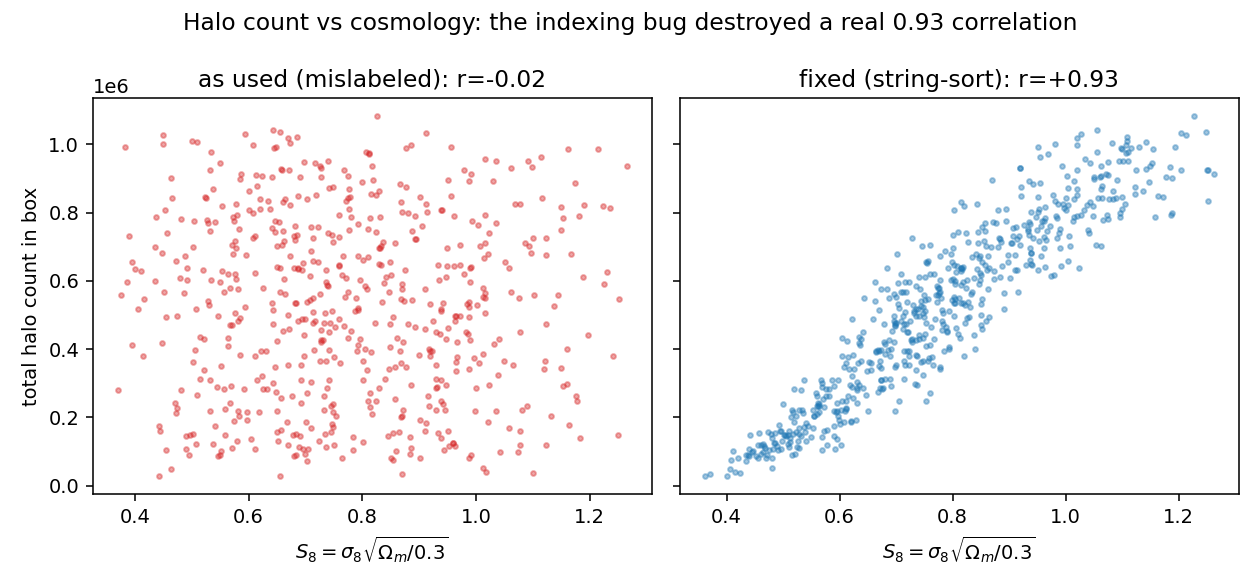
\includegraphics[width=0.85\linewidth]{figures_cmass/labelbug_count_vs_s8.png}
\caption{The indexing bug in one picture. Total halo count in a box against
$S_8 = \sigma_8\sqrt{\Omega_m/0.3}$. As the pipeline used the labels (left) the
correlation is zero; with the string-sort mapping corrected (right) the true
$0.93$ correlation reappears. Halo abundance must track $S_8$, so the left panel
was the signature of a labeling error, not of uninformative data.}
\label{fig:srs-labelbug}
\end{figure}

\paragraph{What this changes, and what it does not.} Every cosmology number we
computed before this point used the labels and is affected; the earlier
cross-fidelity tables have been removed and are replaced by the corrected results
below, and the earlier reading that the SR-versus-LR difference was an irreducible
coin flip was itself a product of the mislabeling. The results that do not use the
labels are unaffected and still stand: the power spectrum match of SR to HR, the
held-out bispectrum, the field-match statistics, the seam test, and the real space
error. The generator conditions on the cosmology as a style vector and was trained
with the scrambled labels, so its conditioning was uninformative during training;
we return to this at the end.

\paragraph{The data is informative after all.} With correct labels the picture
inverts. A halo count in this suite carries a strong cosmological signal: the
total halo count alone correlates with the combination $S_8 = \sigma_8
\sqrt{\Omega_m/0.3}$ at $0.93$ and with $\Omega_m$ at $0.85$. A Fisher forecast on
a single-box power spectrum now explains $98\%$ of the variance, where it
explained $0.2\%$ before, and it constrains $\Omega_m$ and $\sigma_8$ well, with
$\Omega_b$, $h$ and $n_s$ weak or unconstrained, which is the textbook pattern for
a low-redshift halo field. The field-level network tells the same story: after the
fix its predicted $\Omega_m$ correlates with the truth at $0.90$ on both training
and test boxes, where before the fix the correlation was zero and the output was a
constant. So the earlier conclusion that a single box carries almost no cosmology
was an artifact of the labeling, not a property of the data.

\begin{figure}[h]
\centering
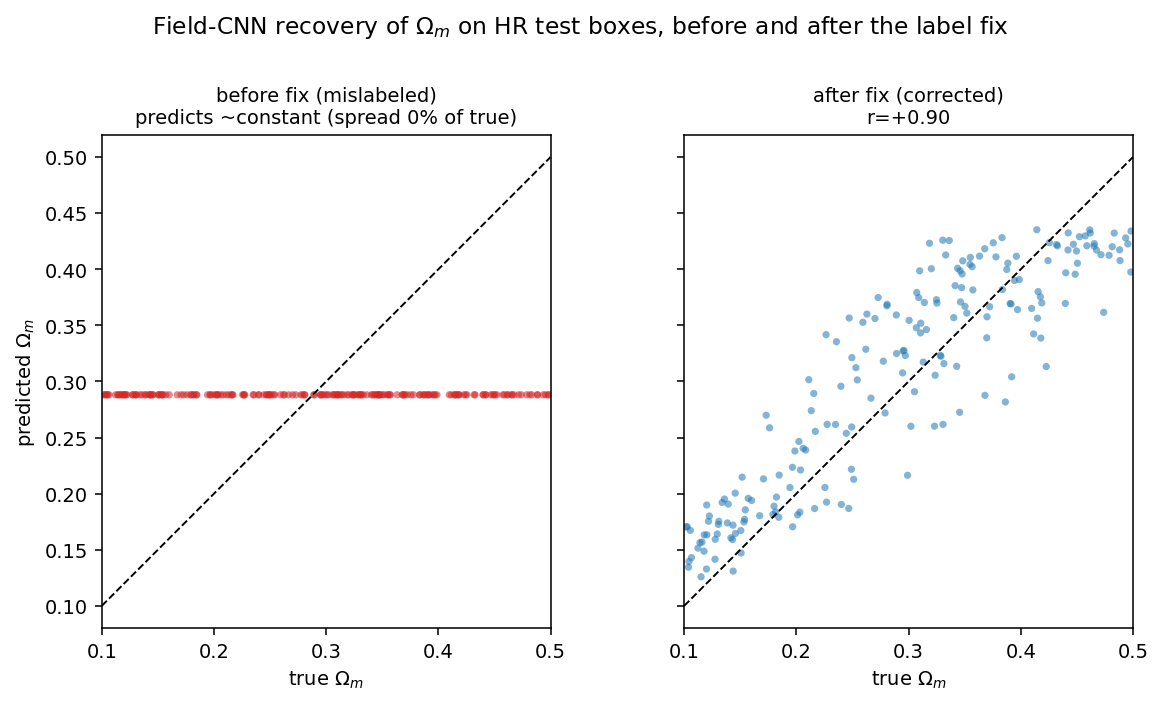
\includegraphics[width=0.82\linewidth]{figures_cmass/field_recovery_Om_cmass.png}
\caption{Field-level CNN recovery of $\Omega_m$ on HR test boxes, before and after
the label fix. Before (left) the prediction is flat and uncorrelated with the
truth (the network returns a near-constant); after (right) it tracks the diagonal
at a correlation of about $0.90$, on both training and test boxes. Same
architecture, same data, only the labels changed.}
\label{fig:srs-recovery}
\end{figure}

\begin{figure}[h]
\centering
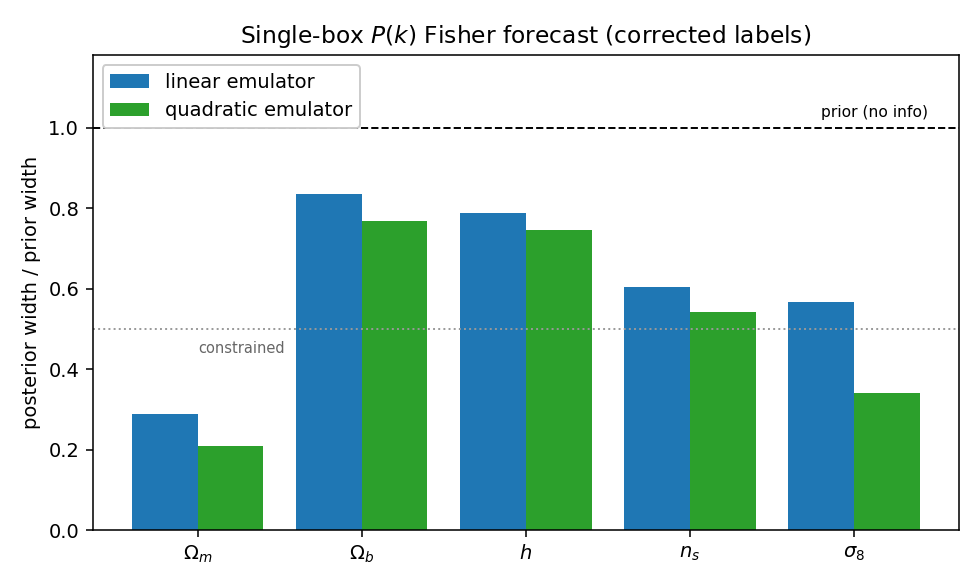
\includegraphics[width=0.72\linewidth]{figures_cmass/fisher_corrected_cmass.png}
\caption{Fisher forecast for a single-box power spectrum with corrected labels:
posterior width divided by prior width per parameter (lower means better
constrained, $1$ means no information). $\Omega_m$ is well constrained and
$\sigma_8$ is constrained, while $\Omega_b$, $h$ and $n_s$ are weak, the textbook
pattern for a low-redshift halo field. Two emulators (linear average slope and
quadratic at the prior centre) bracket the estimate.}
\label{fig:srs-fisher}
\end{figure}

\paragraph{Corrected cross-fidelity, and where SR helps.} We re-ran the goal
metric with correct labels at two levels, the power spectrum summary and the full
field. We train the posterior on one source, apply it to HR, and compare to a
posterior trained on HR, using an ensemble of independently retrained estimators
so the numbers are not single draws. Table~\ref{tab:srs-corrected} gives the
result.
\begin{table}[h]
\centering
\caption{Corrected cross-fidelity KL to HR (posterior trained on the named source,
evaluated on HR), lower is better, with the HR-to-HR floor for reference. Summary
uses the power spectrum; field uses a three-dimensional CNN posterior on the full
box.}
\label{tab:srs-corrected}
\begin{tabular}{lccc}
\toprule
level & LR (raw) & SR & HR floor \\
\midrule
summary $P(k)$ & $0.032$ & $0.088$ & $0.028$ \\
field (CNN)    & $0.49 \pm 0.81$ & $\mathbf{0.024}$ & $0.022$ \\
\bottomrule
\end{tabular}
\end{table}
\begin{figure}[h]
\centering
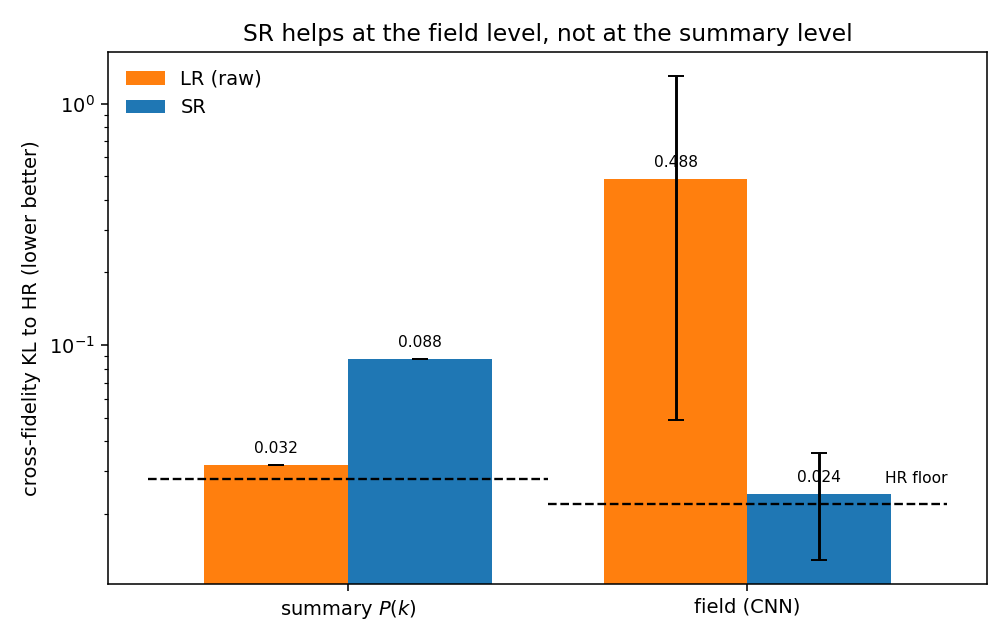
\includegraphics[width=0.7\linewidth]{figures_cmass/crossfid_corrected_cmass.png}
\caption{Corrected cross-fidelity KL to HR (log scale, lower is better) at the two
levels, with the HR-to-HR floor shown as the dashed line. At the summary level the
raw LR field is already at the floor and SR does not help. At the field level, an
LR-trained posterior does not transfer to HR (large and unstable), while an
SR-trained posterior sits at the floor. SR helps exactly where it corrects the
field.}
\label{fig:srs-crossfid-corrected}
\end{figure}
The two levels point in opposite directions, and both make sense. At the summary
level the raw LR power spectrum is already at the HR floor, so an LR-trained
posterior transfers to HR as well as an HR-trained one does, and there is no gap
for SR to close; SR even hurts a little, because the generator reshapes the
small-scale power in a way that does not match how HR responds to cosmology. At
the field level the raw LR box looks different enough from HR that an LR-trained
posterior does not transfer, and it does so unreliably, sometimes acceptably and
sometimes catastrophically, which is why its number carries such a large spread.
SR corrects the field to look like HR, so an SR-trained posterior transfers to HR
reliably, at the floor. This is exactly the deployment case the project is built
on, train the inference model on cheap SR-corrected boxes and apply it to
expensive HR, and at the field level SR makes it work where raw LR does not.

\paragraph{Padding on the goal metric.} We ran the two padding variants through
the corrected cross-fidelity at the summary level as well
(Table~\ref{tab:srs-padding}). Among the SR models the ordering from the earlier
report survives: no padding is best on the goal metric, trim-aware padding is
worse, and trim-unaware is worst, so for the cosmology objective the no-padding
model is the one to use. All three sit above the raw LR control at this level,
consistent with LR already being HR-like on the power spectrum. One number does
change under the fix: the mislabeled data made trim-unaware look catastrophic (a
factor of several hundred above the others), while with correct labels it is the
weakest variant by about a factor of two, not a blow-up. Its real-space error
(Figure~\ref{fig:srs-protocolv2}) remains the clearest and most direct sign that
it is the least reliable model.
\begin{table}[h]
\centering
\caption{Corrected cross-fidelity KL to HR at the summary (power spectrum) level
for the SR padding variants, with the LR control and the HR floor. Lower is
better. Field-level padding numbers are future work.}
\label{tab:srs-padding}
\begin{tabular}{lc}
\toprule
model & summary cross-fidelity KL \\
\midrule
SR, no padding & $\mathbf{0.087}$ \\
SR, trim-aware padding & $0.127$ \\
SR, trim-unaware padding & $0.172$ \\
\midrule
LR (control) & $0.031$ \\
HR floor & $0.028$ \\
\bottomrule
\end{tabular}
\end{table}

\paragraph{Bottom line.} With the labels fixed, the cosmology question has a
clear answer. The data constrains $\Omega_m$ and $\sigma_8$ from a single box. At
the power spectrum level the raw LR field is already HR-like, so SR is not needed
there and slightly hurts. At the field level, which is what SR actually corrects,
an SR-trained posterior transfers to HR at the floor while a raw LR one does not,
so SR provides a real and reliable cosmology benefit exactly where it operates.
Trim-unaware padding is still the weakest variant, worst on the goal metric and
on real-space error, though the label fix shrinks its apparent failure from
catastrophic to about a factor of two. Two honest caveats remain: the
field-level LR number has a wide spread and rests on a handful of retrained
networks, so the size of the gap should be firmed up with more seeds; and because
the generator was trained with the scrambled labels, its cosmology conditioning
was uninformative, so a retrain with correct conditioning may sharpen the SR
result further. Neither caveat changes the direction: with correct labels, SR
helps cosmology at the field level.

\paragraph{A data reliability note.} Partway through these runs, the shared
data storage this project reads from filled up completely, which caused a few
training jobs to fail with a file briefly appearing missing even though it was
not actually deleted. We added a retry step to the data loader and resumed
each affected run from its last saved checkpoint, so no real training progress
was lost. This is a shared infrastructure issue, not a problem with the data or
the method.

\subsection{Files}
\begin{itemize}\itemsep0pt
  \item Data and patching: \texttt{data/patch\_dataset\_cmass.py}
  (shared ops in \texttt{data/patch\_dataset\_real.py})
  \item Model: \texttt{map2map/models/styled\_srsgan.py}
  (\texttt{G\_correct}, \texttt{D\_const})
  \item Training: \texttt{train\_patch\_cmass.py};
  run script \texttt{scripts/train\_patch\_cmass.slurm}
  \item Inference and stitching: \texttt{infer\_stitch\_cmass.py}
  \item Seam eval: \texttt{analysis/eval\_seam\_cmass.py}
  \item Box / per-patch diagnostics: \texttt{analysis/diag\_cmass.py}
  \item SR-vs-HR match stats: \texttt{analysis/match\_stats\_cmass.py}
  \item SR-vs-HR power-spectrum figure: \texttt{analysis/plot\_sr\_vs\_hr.py}
  \item Bispectrum (held-out statistic): \texttt{analysis/bispectrum\_cmass.py}
  \item Training loss curves: \texttt{analysis/plot\_losses\_cmass.py}
  \item Cross-fidelity posterior evaluation: \texttt{evaluate.py} (SR-trained
  or LR-trained posterior evaluated on HR $P(k)$)
  \item Protocol-v2 (no-Pk-loss, padding-variant) training curves:
  \texttt{analysis/plot\_protocolv2\_cmass.py}
  \item Power spectrum on counts: \texttt{analysis/power\_spectrum.py}
  (estimator \texttt{counts}); differentiable training version
  \texttt{analysis/pk\_torch.py}
  \item Posterior and KL: \texttt{inference/nde.py}, \texttt{evaluate.py};
  end-to-end eval \texttt{scripts/eval\_cmass\_wrapper.slurm}
  \item Field-level posterior (three-dimensional CNN, moment-network loss):
  \texttt{models/field\_cnn.py}, \texttt{train\_field\_cnn.py};
  SR field generation \texttt{gen\_sr\_fields.py}; capacity and recovery
  diagnostics \texttt{overfit\_test.py}, \texttt{field\_diag.py}
  \item Outputs: \texttt{runs/patch\_cmass/}; figures: \texttt{figures\_cmass/}
\end{itemize}
.
% Needs the packages main.tex already loads (booktabs, algorithm, algpseudocode,
% listings, xcolor, graphicx). Figures live in figures_cmass/.
% Numbers (updated 2026-09-28, see research_scratch_5.md): summary cross-fid from
% logs/3248394_seedxfid.log (nde_v2, 8 seeds for the main arms) and
% logs/3200801_seedxfid.log (4-seed ablation rows); field cross-fid from
% logs/3248260_fieldev.log (Flow+GAN, 40 epochs), logs/3203212_fieldev.log (20 epochs)
% and the other *_fieldev.log files; scale-by-scale from scratch/why/coh.py
% (COH_SPLIT=test, 200 test boxes); posterior shifts from scratch/why/post_diag_any.py
% (logs/3249151_postdiag.log, logs/3251464_postdiag.log); PQMass, bispectrum and halo
% counts from logs/*_tier1.log; calibration from logs/3251512_spread.log; figures from
% flow_matching/plot_sec7.py. LR here is CHARM (section6_srs.tex calls it FastPM,
% which is wrong).
% =====================================================================

\definecolor{ablgood}{HTML}{1B7F1B}
\newcommand{\abgood}[1]{\textcolor{ablgood}{\textbf{#1}}}

\section{Flow+GAN: Flow Matching Started from the GAN}
\label{sec:flowgan}

This section documents the third model in this work at the same level of detail
as \S\ref{sec:srs}. \S\ref{sec:srs} corrects the LR halo count field with a
styled GAN. The GAN makes the field look like HR, but it is deterministic, and
it biases the summary-level cosmology posterior. Here we keep that GAN and add a
conditional \textbf{flow-matching} model on top of it. The flow starts from the
GAN's output plus noise and learns to turn it into a sample of the HR field. We
call the combined model \textbf{Flow+GAN}. The section ends with a table of
every model and ablation we ran on this data (\S\ref{sec:flowgan-ablations}).

\paragraph{Goal.} The goal is the same as in \S\ref{sec:srs}. At inference the
model sees only the cheap LR field and must produce an SR field that behaves like
HR. We grade it the same way: a posterior trained on SR fields is applied to HR
fields, and we measure how far its answer is from a posterior trained on HR
(cross-fidelity KL). HR is used only for training and grading.

\paragraph{Why a new model: what the GAN and a plain flow get wrong.} Two
findings from the previous section and its follow-ups motivate this design.
\begin{itemize}
  \item \textbf{The GAN is deterministic and tilts the power spectrum.} Its
  learned noise strength is about $2\times10^{-4}$, so ten noise draws give the
  same field. Its $L_1$ term pulls each voxel toward the conditional median.
  This shrinks the large-scale contrast (about $5\%$ less power at $k<0.06\,h\,\mathrm{Mpc}^{-1}$)
  and adds $1$ to $3\%$ power at high $k$. A posterior reads this tilt as a
  shift in $\sigma_8$: on HR test boxes the GAN-trained posterior's $\sigma_8$ mean
  is off by about one HR posterior width. That is why the deployed GAN's summary
  cross-fidelity KL ($0.202$) is worse than raw LR ($0.049$). One fixed per-$k$
  calibration curve on the GAN's training $P(k)$ brings it to $0.068$, which
  shows the problem is this tilt, not missing information.
  \item \textbf{A plain flow samples, but loses the large scales.} A flow that
  starts from pure Gaussian noise (``Flow'' below) has no $\sigma_8$ bias and
  reaches $0.087$. But it rebuilds every scale from noise, including the largest
  ones, which LR already gets right. Its large-scale power scatters more from box
  to box than LR's. Its coherence with HR at $k\approx0.125$ falls below LR's.
  Its predictions are also too narrow: HR usually falls outside the spread of its
  draws (spread-skill ratio $0.20$, ideal $1$).
\end{itemize}
Flow+GAN takes the part each model gets right. The GAN supplies the large-scale
structure and a best guess. The flow adds only what the best guess cannot
predict, and it adds it as a sample, not as a mean. This follows residual
diffusion for downscaling (CorrDiff, Mardani et al.\ 2023, arXiv:2309.15214),
stochastic flow matching for super-resolution (Fotiadis et al.\ 2024,
arXiv:2410.19814), and stochastic interpolants with a data-dependent start
(Albergo et al.\ 2023, arXiv:2310.03725).

\paragraph{Terminology.} \textbf{GAN} means the deployed generator of
\S\ref{sec:srs}: Arm A (pad $0$), power-spectrum loss off, trained with correct
cosmology labels, run at the fiducial cosmology (tag \texttt{Afixfid}).
\textbf{Flow} means the pure-noise flow matcher trained on $64^3$ patches (tag
\texttt{fm\_gauss\_nodq}). \textbf{Flow+GAN} is the model of this section. As in
\S\ref{sec:srs}, we use LR/LF and HR/HF interchangeably.

\subsection{Data Preprocessing}
\textit{Source: \texttt{cmass-ili}; loaders \texttt{flow\_matching/data.py}
(\texttt{FullBoxDataset}), model space \texttt{flow\_matching/space.py}.}

\paragraph{Input.} The data is the same as in \S\ref{sec:srs}: $2000$ paired
halo count grids of $128^3$ cells on a periodic $1000\,h^{-1}\mathrm{Mpc}$ box at
$z=0.5$, with LR from CHARM and HR from Quijote N-body, and the same
$1600/200/200$ train/validation/test split. One extra input is new. Before
training, we run the GAN once on every one of the $2000$ LR boxes, at the
fiducial cosmology, and store its output (\texttt{sr\_fields/Afix\_fiducial}).
The GAN is frozen from here on; it is not trained further.

\paragraph{Model space.} The flow works on a standardised log count,
\begin{equation}
  y = \frac{\log(1+n) - \mu}{s}, \qquad
  n = \mathrm{round}\big(\exp(s\,y+\mu) - 1\big) \ \ \text{clamped to } [0, 200],
  \label{eq:fg-space}
\end{equation}
where $\mu=0.152$ and $s=0.359$ are the mean and standard deviation of
$\log(1+n_\text{HR})$ over $50$ training boxes. The LR field, the GAN field and
the HR target all use this same map. We do \emph{not} dequantise (add uniform
noise to the integer counts before the log). An earlier flow that did so
(\texttt{fm\_gauss}) needed a floor decoder, and noise near the empty-cell
boundary made spurious halos: about $9\%$ too many halos, and a summary KL of
$0.244$. The rounding decoder in Eq.~\ref{eq:fg-space} does not have this bias.
Power spectra are computed exactly as in \S\ref{sec:srs}, on the physical-count
overdensity $\delta = n/\bar n - 1$ with the per-box mean.

\subsection{Data Pipeline (full box, no patches)}
\textit{Located in: \texttt{flow\_matching/data.py},
\texttt{flow\_matching/augment.py}, \texttt{flow\_matching/train\_fm.py}.}

Unlike the GAN and the earlier flows, Flow+GAN is trained and sampled on the
\textbf{whole $128^3$ box at once}. The patch pipeline of \S\ref{sec:srs} cuts
each box into eight $64^3$ cores. For a model that draws fresh noise per patch,
this matters: each patch gets its own noise. Modes longer than a patch are then
re-drawn independently in each patch, and the circular padding treats a patch as
periodic when it is not. Sampling the old patch-trained flow on the full box
already raised its coherence with HR at $k=0.125$ from $0.36$ to $0.67$. The
velocity network is fully convolutional with circular padding, so it runs on
$128^3$ without change, and the box is truly periodic, so circular padding is
exact.

Each training item is one box: the LR counts, the HR counts and the GAN output,
all $128^3$. Two augmentations are applied identically to all three fields:
\begin{itemize}
  \item \textbf{Random periodic shift.} The three fields are rolled by the same
  random offset along each axis. Because the box is periodic this is an exact
  symmetry, and it stops the network from learning fixed positions.
  \item \textbf{Cube symmetries.} One of the $48$ rotations and reflections of
  the cube (\texttt{--aug full48}).
\end{itemize}

\begin{table}[t]
\centering
\caption{Notation for the Flow+GAN pipeline.}
\label{tab:fg-notation}
\begin{tabular}{llp{7.0cm}}
\toprule
Symbol & Value & Meaning \\
\midrule
$N$ & $128$ & box side in voxels (the model sees the whole box) \\
$y_\text{LR},\,y_\text{GAN},\,y_\text{HR}$ & $(1,128^3)$ & LR, GAN and HR fields in model space (Eq.~\ref{eq:fg-space}) \\
$\sigma_z$ & $0.920$ & RMS of $y_\text{HR}-y_\text{GAN}$ over $50$ training boxes ($64^3$ patches) \\
$t$ & $[0,1]$ & flow time; $t{=}0$ is the noisy GAN field, $t{=}1$ is HR \\
$x_t$ & $(1,128^3)$ & point on the straight path between source and target \\
$v_\phi$ & $17.4$M params & velocity network (3D UNet) \\
\bottomrule
\end{tabular}
\end{table}

\subsection{Model: Input/Output Specification}
\textit{Implementation: \texttt{flow\_matching/interpolant.py}
(\texttt{Interpolant}, source \texttt{gan\_white}),
\texttt{flow\_matching/unet3d.py}.}

\paragraph{The path.} Flow matching learns a velocity field that carries a
\emph{source} sample $x_0$ to a \emph{target} sample $x_1$ along a straight line.
For Flow+GAN the source is the GAN's field plus white noise at the size of the
GAN's typical error, and the target is HR:
\begin{equation}
  x_0 = y_\text{GAN} + \sigma_z\,\boldsymbol\epsilon,\quad
  \boldsymbol\epsilon\sim\mathcal N(0,I), \qquad
  x_1 = y_\text{HR}, \qquad
  x_t = (1-t)\,x_0 + t\,x_1 .
  \label{eq:fg-path}
\end{equation}
The velocity along this line is constant, $x_1-x_0$. The network is trained to
predict it:
\begin{equation}
  \mathcal L_\text{FM} \;=\; \mathbb E_{t,\,\boldsymbol\epsilon,\,\text{box}}
    \big\lVert v_\phi\big(x_t,\,t,\,[y_\text{LR},\,y_\text{GAN}]\big) - (x_1 - x_0)\big\rVert_2^2 ,
  \qquad t\sim\mathcal U[0,1].
  \label{eq:fg-loss}
\end{equation}
This is the only loss. There is no adversarial term, no $L_1$ term and no
power-spectrum term.

\paragraph{Why start from the GAN.} With a pure-noise source ($x_0\sim\mathcal
N(0,I)$) the flow must create every scale, including the large scales that LR
and the GAN already get right. Starting at the GAN field means the flow's job is
only the residual $y_\text{HR}-y_\text{GAN}$, whose size is $\sigma_z$. The noise
$\sigma_z\boldsymbol\epsilon$ is what makes the model stochastic: with
$\sigma_z=0$ the flow would be a deterministic map and could return only one
field per LR box, which is the GAN's failure again. The noise is white, so it
has little power at large scales, and the large-scale modes of the start point
are essentially the GAN's.

\paragraph{Conditioning.} The network sees the current state $x_t$ and two
conditioning channels, the LR field and the GAN field, concatenated as input
channels ($3$ input channels in total). It does \emph{not} see the cosmology
vector: the flow is $\theta$-independent. The only $\theta$ in the pipeline is
the fixed fiducial value given to the frozen GAN, so no per-box cosmology can
leak into the SR fields.

\begin{table}[t]
\centering
\caption{Tensors consumed/produced by the velocity network for one box (batch
dimension omitted).}
\label{tab:fg-io}
\begin{tabular}{lll}
\toprule
Symbol & Shape & Meaning \\
\midrule
$x_t$ & $(1,128,128,128)$ & current state on the path (Eq.~\ref{eq:fg-path}) \\
$y_\text{LR}$ & $(1,128,128,128)$ & LR field, model space (conditioning) \\
$y_\text{GAN}$ & $(1,128,128,128)$ & frozen GAN output, model space (conditioning and start point) \\
$t$ & scalar & flow time, sinusoidal embedding \\
$v_\phi(\cdot)$ & $(1,128,128,128)$ & predicted velocity \\
\bottomrule
\end{tabular}
\end{table}

\paragraph{Velocity network.} $v_\phi$ is a 3D UNet with $17.4$M parameters.
\begin{enumerate}
  \item Every convolution is $3{\times}3{\times}3$ with circular padding, so the
  network is exactly shift-equivariant on the periodic box.
  \item Four levels at full, $1/2$, $1/4$ and $1/8$ resolution with channel
  widths $32\cdot(1,2,4,4)$, two residual blocks per level, GroupNorm, and one
  self-attention block at the coarsest level for global context.
  \item The time $t$ enters through a sinusoidal embedding and an MLP that sets a
  per-channel scale and shift after each GroupNorm (FiLM).
  \item The last convolution is initialised to zero, so the initial velocity is
  about $0$.
\end{enumerate}
Training keeps an exponential moving average (EMA, decay $0.999$) of the weights;
validation and sampling use the EMA weights.

\subsection{Training Step}
\textit{Located in: \texttt{flow\_matching/train\_fm.py}.}

\begin{algorithm}[H]
\caption{Flow+GAN training step (one box)}
\label{alg:fg-train}
\begin{algorithmic}[1]
\Require LR counts $\mathbf L$, HR counts $\mathbf H$, frozen GAN output $\mathbf G$ (all $128^3$), $\sigma_z$
\State draw one random periodic shift and one of $48$ cube symmetries; apply both to $\mathbf L,\mathbf H,\mathbf G$
\State $y_\text{LR},y_\text{HR},y_\text{GAN}\gets$ Eq.~\ref{eq:fg-space} applied to $\mathbf L,\mathbf H,\mathbf G$
\State $\boldsymbol\epsilon\sim\mathcal N(0,I)$, \ $t\sim\mathcal U[0,1]$
\State $x_0\gets y_\text{GAN}+\sigma_z\boldsymbol\epsilon$, \ $x_t\gets(1-t)x_0+t\,y_\text{HR}$
\State $\mathcal L\gets\big\lVert v_\phi(x_t,t,[y_\text{LR},y_\text{GAN}])-(y_\text{HR}-x_0)\big\rVert^2$ \Comment{mean over voxels}
\State update $\phi$ (AdamW, linear warm-up $500$ steps, grad-clip $1$, bf16); update EMA
\end{algorithmic}
\end{algorithm}

\paragraph{Validation and checkpoint selection.} After each epoch we generate
$2$ draws for each of the first $16$ validation boxes ($16$ Heun steps) and
compute, in $\log(1+n)$ space: the $L_1$ error per voxel, the fair
\textbf{CRPS} of the $2$-draw ensemble, the spread between draws, the
total-count error, and the $P(k)$ RMS against HR. For $K$ draws $s_1,\dots,s_K$
and the true value $h$, the per-voxel fair CRPS is
\begin{equation}
  \mathrm{CRPS} = \frac1K\sum_{i}|s_i-h| - \frac{1}{2K(K-1)}\sum_{i\neq j}|s_i-s_j| .
  \label{eq:fg-crps}
\end{equation}
The first term rewards draws close to HR; the second rewards draws that differ
from each other. So CRPS, unlike $L_1$, does not favour a blurred mean field.
\texttt{best.pt} is the epoch with the lowest validation CRPS. We fixed this rule
before training. $P(k)$ is only a check: it is never trained on and never used
to select.

\subsection{Inference}
\textit{Located in: \texttt{flow\_matching/sample\_fm.py},
\texttt{flow\_matching/common.py} (\texttt{generate\_box}).}

For one box: run the frozen GAN on LR (already stored), build the start point
$x_0$, integrate the learned velocity from $t=0$ to $t=1$ with Heun's
second-order method, and map back to counts. The noise is seeded by the box index
and draw number, so every output can be reproduced.

\begin{algorithm}[H]
\caption{Flow+GAN inference (one box, one draw)}
\label{alg:fg-infer}
\begin{algorithmic}[1]
\Require LR box $\mathbf L$, GAN output $\mathbf G$, trained $v_\phi$ (EMA), $\sigma_z$, steps $S{=}32$, seed
\State $y_\text{LR},y_\text{GAN}\gets$ Eq.~\ref{eq:fg-space}; \ $x\gets y_\text{GAN}+\sigma_z\boldsymbol\epsilon$ \Comment{seeded $\boldsymbol\epsilon$}
\For{$i=0,\dots,S-1$} \Comment{$t_i=i/S$, $\Delta t = 1/S$}
  \State $v_0\gets v_\phi(x,t_i,[y_\text{LR},y_\text{GAN}])$
  \If{$i<S-1$}
    \State $v_1\gets v_\phi(x+\Delta t\,v_0,\,t_{i+1},[y_\text{LR},y_\text{GAN}])$; \ $x\gets x+\tfrac12\Delta t\,(v_0+v_1)$ \Comment{Heun}
  \Else
    \State $x\gets x+\Delta t\,v_0$ \Comment{Euler on the last step}
  \EndIf
\EndFor
\State \Return $\mathrm{round}\big(\exp(s\,x+\mu)-1\big)$, clamped to $[0,200]$ \Comment{integer counts}
\end{algorithmic}
\end{algorithm}

\paragraph{No stitching.} Because the whole box is generated at once, there are
no cores, no halo and no seams. The stitching step of \S\ref{sec:srs} does not
apply.

\subsection{Evaluation}
\label{sec:fg-eval}
\textit{Located in: \texttt{evaluate.py}, \texttt{inference/nde.py},
\texttt{analysis/seed\_xfid\_check.py}, \texttt{eval\_field\_crossfid.py},
\texttt{scratch/why/coh.py}, \texttt{flow\_matching/plot\_sec7.py}.}

We use the metrics of \S\ref{sec:srs-eval}: the power spectrum, the transfer
$T(k)=P_X/P_\text{HR}$, the cross-coherence $r(k)$ with HR
(Eq.~\ref{eq:srs-Tr}), and cross-fidelity KL (Eq.~\ref{eq:srs-kl}) at two levels.
One thing changed in the summary-level protocol, so the numbers below are not
directly comparable to Table~\ref{tab:srs-corrected}:
\begin{itemize}
  \item \textbf{Summary level (protocol v2).} The NDE input is $\log_{10}P(k)$ in
  $29$ bins. The three lowest of the original $32$ bins contain no Fourier modes,
  and we now drop them. We train $8$ NDE seeds for each of the main sources (HR,
  LR, GAN, Flow and every Flow+GAN checkpoint) and $4$ for the other ablations.
  For seed $s$ we compare $q_X^{(s)}$ with $q_\text{HR}^{(s)}$ on the $200$ HR test
  boxes and report the mean $\pm$ standard deviation over seeds. The HR floor is
  the KL between independently trained HR posteriors. This per-seed protocol is
  stricter than the ensemble protocol of \S\ref{sec:srs-correction}: LR is $0.049$
  here versus $0.032$ there. The ranking of the GAN arms is the same under both.
  \item \textbf{Field level.} Unchanged from \S\ref{sec:srs-correction}: a 3D CNN
  posterior on the full box, $3$ CNN seeds trained on SR, evaluated on HR test
  boxes against $6$ HR-trained reference CNNs. The same $8$ LR CNNs and $6$ HR
  CNNs are reused for every arm.
\end{itemize}

\subsection{Best-Run Configuration}
\textit{Run script: \texttt{scratch/why/train\_v2\_1gpu.slurm} (resumes automatically
from \texttt{last.pt}, so the same script ran epochs $0$ to $19$ and $20$ to $39$); checkpoint
\texttt{models/Flow+GAN/best\_crps40\_epoch39.pt}; sampling \texttt{scratch/why/gen\_v2.slurm}.}

\begin{lstlisting}[language=bash]
--source gan_white                        # python -m flow_matching.train_fm
--extra-dir sr_fields/Afix_fiducial     # frozen GAN output: start point + 2nd cond channel
--full-box --roll --aug full48          # whole periodic box, random shift + 48 symmetries
--no-dequant                            # round decoder
--base-ch 32 --ch-mult 1,2,4,4 --attn-levels 3    # 17.4M-param UNet
--lr 1e-4 --warmup 500 --ema 0.999 --grad-clip 1.0 --amp bf16
--epochs 40 --select crps --val-max-sims 16 --val-draws 2 --val-steps 16
# sampling: --steps 32 --method heun (full box, EMA weights, seeded per box)
\end{lstlisting}

The run used one GH200 GPU (about $13.5$ minutes per epoch, batch of one box).
Epochs are numbered from $0$, as in the training log. We first stopped the run
after $20$ epochs, because validation CRPS had been flat since epoch $11$; that
run's CRPS-best checkpoint was epoch $15$. The validation $P(k)$ error was still
falling, so we resumed the same run, with the same recipe, weights, EMA and optimizer state,
to the planned $40$ epochs. Before looking at any test result we fixed which
checkpoints to report: the CRPS-best one (epoch $38$, the one we use below) and the
final one (epoch $39$). Validation at those epochs:

\begin{center}
\begin{tabular}{lccccc}
\toprule
model & $L_1$/voxel & CRPS & spread & count error & $P(k)$ RMS \\
\midrule
Flow+GAN, epoch 15 (first $20$ epochs) & $0.146$ & $0.0749$ & $0.071$ & $+0.2\%$ & $0.059$ \\
Flow+GAN, epoch 38 (CRPS-best of $40$) & $0.144$ & $\mathbf{0.0740}$ & $0.070$ & $-1.6\%$ & $\mathbf{0.052}$ \\
Flow+GAN, epoch 39 (final) & $0.143$ & $\mathbf{0.0740}$ & $0.069$ & $-1.5\%$ & $0.053$ \\
Flow from noise, full box (control) & $0.195$ & $0.100$ & -- & $+3.2\%$ & $0.084$ \\
\bottomrule
\end{tabular}
\end{center}
The control row is the same recipe with a pure-noise source instead of the GAN,
read at epoch $7$ to $8$ for comparison (its later epochs were unstable). Flow+GAN
is better on every validation metric. The second $20$ epochs improve CRPS only
slightly ($0.0749\to0.0740$, flat from epoch $30$), but they reduce the $P(k)$ error
($0.059\to0.052$), even though $P(k)$ is not in the loss. The validation count error
is measured on only $16$ boxes and moves by about $1\%$ from epoch to epoch.

\subsection{Results}
\label{sec:fg-results}

\paragraph{1. Power spectrum: the tilt is gone.} Figure~\ref{fig:fg-pk} and
Table~\ref{tab:fg-scale} compare the power spectrum and cross-coherence of LR,
the GAN, the Flow and Flow+GAN against HR. Flow+GAN's median power is within
$1.4\%$ of HR at every scale ($0.986$ to $1.009$). The median transfer deviates
from $1$ by $1.1\%$ RMS, against $2.7\%$ for raw LR, $4.4\%$ for the GAN and
$6.1\%$ for the Flow. The GAN's pattern (too little power at large scales, too
much at small scales) is removed, and so is the Flow's $3$ to $4\%$ deficit at
most scales. The cross-coherence with HR is above LR at every scale except the
largest ($r=0.76$ vs $0.51$ at $k\approx0.125$, $0.34$ vs $-0.13$ at
$k\approx0.35$). It stays below the GAN's, which is expected: a sampler draws
the unpredictable small-scale structure fresh, while the GAN returns its
single best guess.

\begin{figure}[t]
\centering
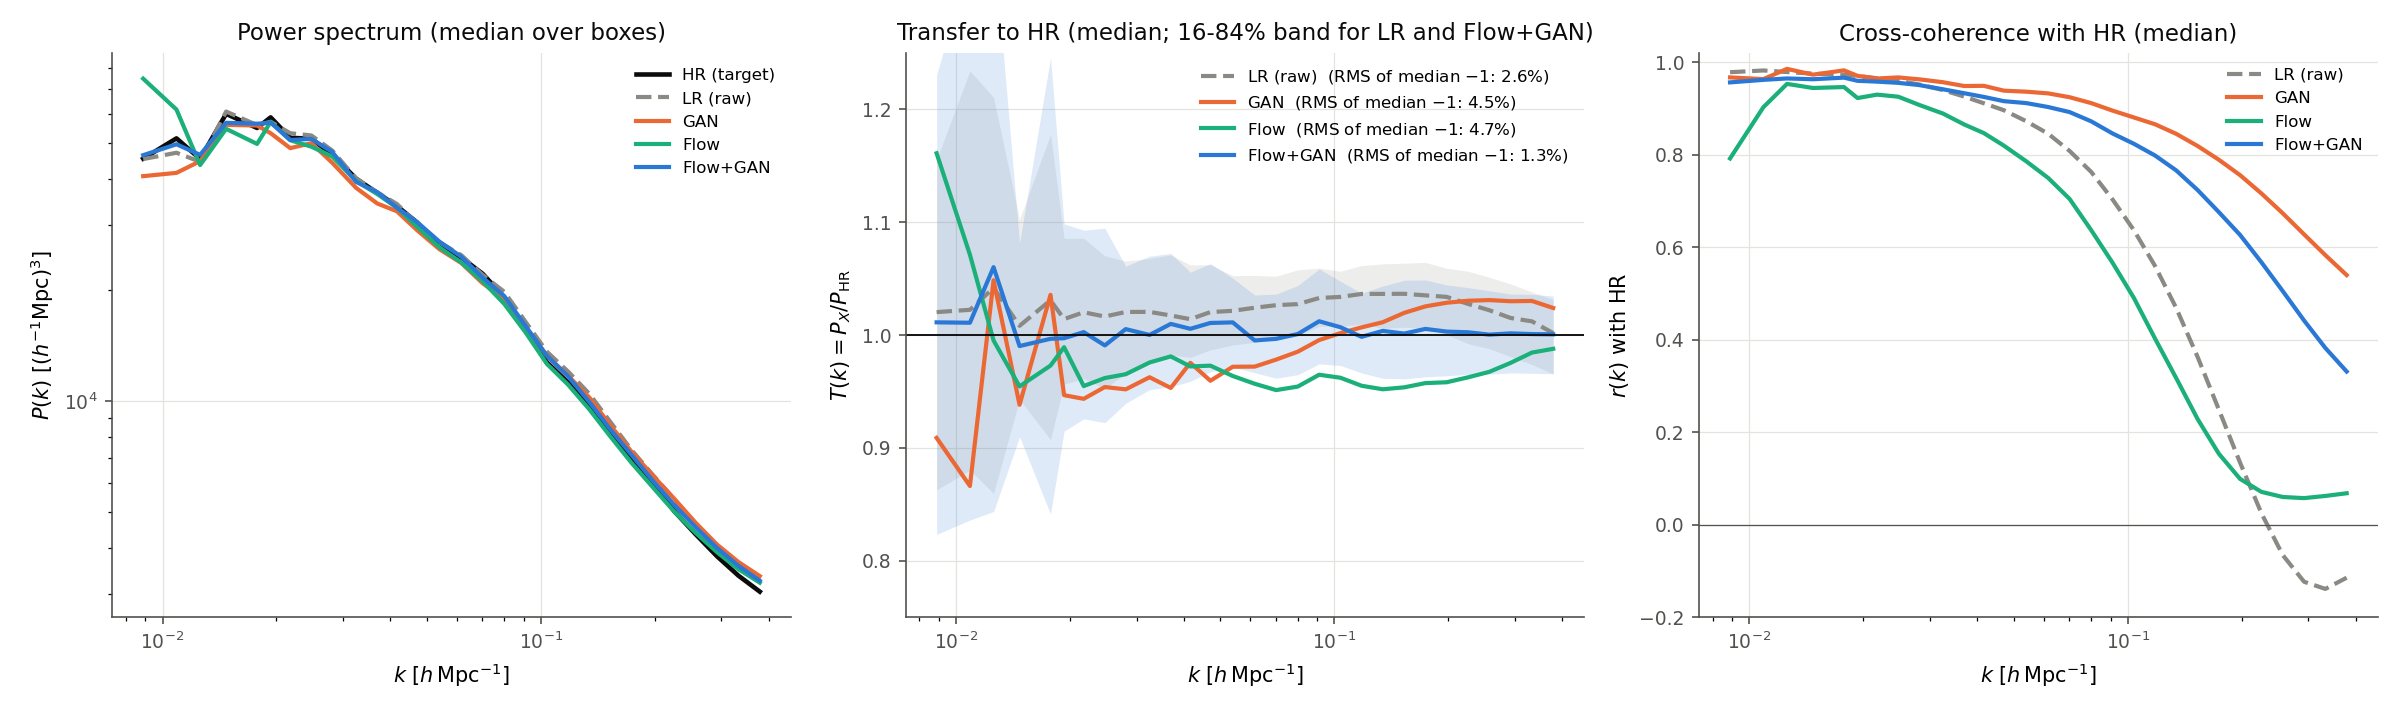
\includegraphics[width=\linewidth]{figures_cmass/pk_panel_box_flowgan.png}
\caption{Full-box diagnostic on $100$ validation boxes. Flow+GAN has no
test-split fields yet, and the first $16$ validation boxes (in sorted order)
were used for checkpoint selection, so we use the next $100$.
\textbf{Left:} median $P(k)$ of HR, LR, GAN, Flow and Flow+GAN.
\textbf{Middle:} transfer $T(k)=P_X/P_\text{HR}$, median, with the 16 to 84
percentile band for LR and Flow+GAN; the legend gives the RMS deviation of the
median from $1$. The GAN (orange) is low at large scales and high at small
scales; the Flow (green) is low at all scales; Flow+GAN (blue) stays on $1$.
\textbf{Right:} cross-coherence $r(k)$ with HR. Flow+GAN is above LR from
$k\approx0.05$ onward and below the deterministic GAN.}
\label{fig:fg-pk}
\end{figure}

\begin{table}[t]
\centering
\caption{Scale by scale, the first $100$ validation boxes, in wide $k$ bands
centred on the listed values. $P/P_\text{HR}$: median power
ratio to HR ($1$ is right). Scatter: box-to-box standard deviation of that ratio
(LR is the reference). $r$: median cross-coherence with HR ($1$ is best).}
\label{tab:fg-scale}
\small
\begin{tabular}{l cccc cc cccc}
\toprule
 & \multicolumn{4}{c}{$P/P_\text{HR}$ median} & \multicolumn{2}{c}{scatter} & \multicolumn{4}{c}{$r$ with HR} \\
\cmidrule(lr){2-5}\cmidrule(lr){6-7}\cmidrule(lr){8-11}
$k$ [$h\,\mathrm{Mpc}^{-1}$] & $0.013$ & $0.042$ & $0.125$ & $0.35$ & $0.013$ & $0.125$ & $0.013$ & $0.042$ & $0.125$ & $0.35$ \\
\midrule
LR (raw)  & $1.009$ & $1.017$ & $1.037$ & $1.007$ & $\mathbf{0.20}$ & $0.34$ & $\mathbf{0.975}$ & $0.908$ & $0.508$ & $-0.126$ \\
GAN       & $0.949$ & $0.962$ & $1.010$ & $1.029$ & $\mathbf{0.20}$ & $0.34$ & $0.974$ & $\mathbf{0.944}$ & $\mathbf{0.850}$ & $\mathbf{0.559}$ \\
Flow      & $1.057$ & $0.970$ & $0.959$ & $0.989$ & $0.40$ & $\mathbf{0.32}$ & $0.907$ & $0.837$ & $0.358$ & $0.062$ \\
Flow+GAN  & $\mathbf{0.986}$ & $\mathbf{1.004}$ & $\mathbf{0.998}$ & $\mathbf{1.009}$ & $0.29$ & $0.35$ & $0.964$ & $0.921$ & $0.760$ & $0.339$ \\
\bottomrule
\end{tabular}
\end{table}

\paragraph{2. Cross-fidelity: Flow+GAN matches LR at the summary level and stays near the floor at the field level.}
Figure~\ref{fig:fg-crossfid} and Table~\ref{tab:fg-crossfid} give the goal
metric. At the summary level the $40$-epoch Flow+GAN reaches $0.047\pm0.008$,
against $0.049\pm0.010$ for raw LR. Compared seed by seed (same NDE seed, same HR
reference posterior), the difference from LR averages $-0.001$. It is the first
SR model that is not worse than LR at the summary level: the GAN is at $0.202$
and the Flow at $0.087$. The final checkpoint (epoch $39$) gives $0.055\pm0.011$,
also equal to LR within noise. At the field level Flow+GAN reaches $0.027\pm0.011$,
close to the HR floor ($0.019$), while the LR-trained CNN posterior does not
transfer reliably ($0.47\pm0.78$).

Two cautions apply. First, epochs $38$ and $39$ are neighbouring checkpoints of one
run, yet their summary KLs differ by $0.008$, about one seed standard deviation.
So the fair claim is that Flow+GAN is equal to LR within noise, not that it beats
LR. Second, the $20$-epoch model (epoch $15$) was at $0.065\pm0.011$. The
improvement from longer training is therefore real but modest, and it is of the
same order as the checkpoint-to-checkpoint noise.

\begin{figure}[t]
\centering
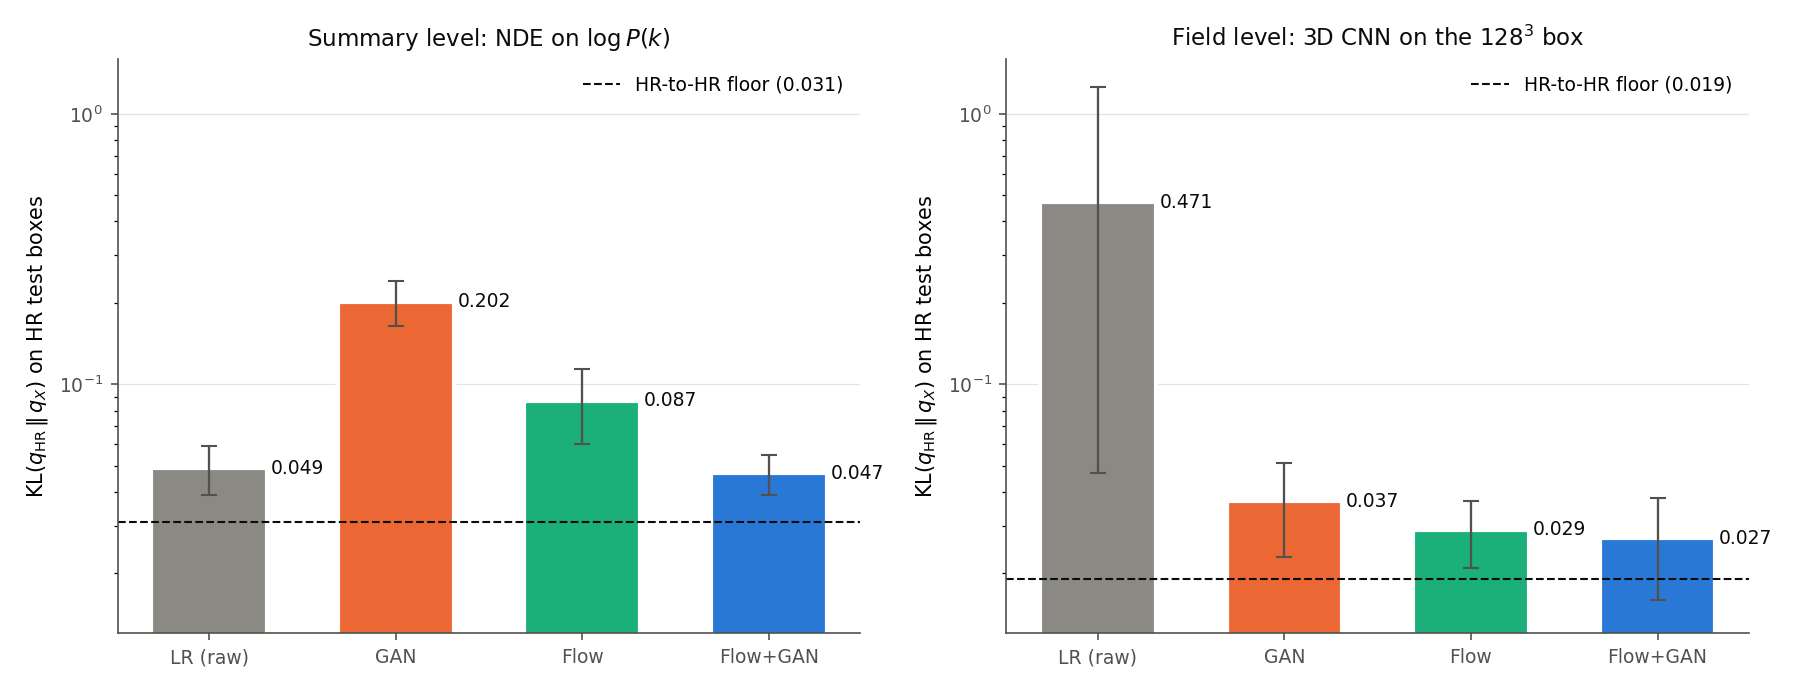
\includegraphics[width=0.95\linewidth]{figures_cmass/crossfid_flowgan.png}
\caption{Cross-fidelity KL to HR (log scale, lower is better), posterior trained
on source $X$ and applied to the $200$ HR test boxes. Dashed: HR-to-HR floor.
Flow+GAN is the $40$-epoch model (CRPS-best checkpoint).
\textbf{Left:} summary level ($P(k)$ NDE, protocol v2, mean $\pm$ std over $8$
seeds). Flow+GAN ($0.047$) equals raw LR ($0.049$); the GAN is at $0.202$ and the
Flow at $0.087$. \textbf{Right:} field level (3D CNN). All three SR models are
near the floor, Flow+GAN ($0.027$) closest; LR does not transfer reliably.}
\label{fig:fg-crossfid}
\end{figure}

\begin{table}[t]
\centering
\caption{Cross-fidelity KL to HR, lower is better. Summary: protocol v2, mean
$\pm$ std over $8$ NDE seeds, $200$ HR test boxes. Field: mean $\pm$ std over
HR-reference $\times$ SR-replicate pairs. Best SR value per column in bold.}
\label{tab:fg-crossfid}
\begin{tabular}{lcc}
\toprule
source & summary $P(k)$ & field (CNN) \\
\midrule
LR (raw, control) & $0.049\pm0.010$ & $0.471\pm0.782$ \\
GAN (deployed)    & $0.202\pm0.038$ & $0.037\pm0.014$ \\
Flow (noise start, patches) & $0.087\pm0.027$ & $0.029\pm0.008$ \\
Flow+GAN, epoch 15 ($20$-epoch run) & $0.065\pm0.011$ & $\mathbf{0.024\pm0.009}$ \\
Flow+GAN, epoch 38 (CRPS-best of $40$) & $\mathbf{0.047\pm0.008}$ & $0.027\pm0.011$ \\
Flow+GAN, epoch 39 (final) & $0.055\pm0.011$ & $0.027\pm0.015$ \\
\midrule
HR floor          & $0.031\pm0.009$ & $0.019$ \\
\bottomrule
\end{tabular}
\end{table}

\paragraph{3. Why it works: the posterior shifts.} Table~\ref{tab:fg-s8}
measures directly how each SR-trained posterior differs from the HR-trained one.
For each HR test box and seed we take the SR-trained posterior mean minus the
HR-trained posterior mean, in units of the HR posterior's standard deviation. We
report the mean over boxes (bias) and the standard deviation over boxes (scatter),
averaged over the $8$ seeds, for the two parameters the $P(k)$ posterior
constrains best, $\Omega_m$ and $\sigma_8$. The GAN's problem is a single one:
its $\sigma_8$ is biased by a full posterior width. After $20$ epochs Flow+GAN has
no such bias beyond LR's own ($+0.23$ vs $+0.18$), but its $\Omega_m$ scatter is
larger than LR's ($0.22$ vs $0.17$). After $40$ epochs the $\sigma_8$ bias is gone
($-0.01$) and the $\Omega_m$ scatter has dropped to $0.18$, close to LR. The same
pattern holds for $n_s$ (scatter $0.34\to0.30$, LR $0.27$). These are the changes
that close the summary gap. The per-box scatter of $\sigma_8$ was never the
problem: it is at LR's level for every Flow+GAN checkpoint. The final checkpoint
(epoch $39$) has a $\sigma_8$ bias of $+0.17$, which is again LR's level, which
shows how much this quantity moves between neighbouring checkpoints.

\begin{table}[h]
\centering
\caption{Shift of the posterior mean on HR test boxes (SR-trained minus
HR-trained), in units of the HR posterior standard deviation; $200$ boxes
$\times$ $8$ seeds. Bias is the mean over boxes, scatter the standard deviation
over boxes. $0$ is ideal for all columns.}
\label{tab:fg-s8}
\begin{tabular}{lcccc}
\toprule
 & \multicolumn{2}{c}{$\Omega_m$} & \multicolumn{2}{c}{$\sigma_8$} \\
\cmidrule(lr){2-3}\cmidrule(lr){4-5}
source & bias & scatter & bias & scatter \\
\midrule
LR (raw)  & $+0.01$ & $\mathbf{0.17}$ & $+0.18$ & $0.38$ \\
GAN (deployed) & $-0.11$ & $0.18$ & $+1.06$ & $0.52$ \\
Flow (patches) & $+0.02$ & $0.21$ & $-0.10$ & $0.46$ \\
Flow+GAN, epoch 15 & $-0.02$ & $0.22$ & $+0.23$ & $0.39$ \\
Flow+GAN, epoch 38 & $+0.03$ & $0.18$ & $\mathbf{-0.01}$ & $0.37$ \\
Flow+GAN, epoch 39 & $+0.01$ & $0.18$ & $+0.17$ & $\mathbf{0.36}$ \\
\bottomrule
\end{tabular}
\end{table}

\paragraph{4. Distribution checks beyond the posterior.} We also ran the
field-level checks of \S\ref{sec:srs} on the $40$-epoch model.
\begin{itemize}
  \item \textbf{PQMass} ($200$ validation boxes, one-point count histogram, as in
  \S\ref{sec:srs}). Flow+GAN at epoch $38$ gives $\chi^2/\text{dof}=1.20$, against
  $0.83$ for LR and $2.22$ for the GAN, so its one-point distribution is close to
  statistically indistinguishable from HR. The $20$-epoch model failed this test
  ($3.59$). We traced that failure to the flow itself: at a fixed total halo count
  it produced about $2\%$ too few cells with two halos and too many with three, and
  $3$ times too many cells with more than $20$ halos. The decoder was not the cause:
  rounding in log space instead of count space changed nothing ($3.65$), and
  thresholds matched to HR's histogram on training boxes moved the total count by
  $9\%$ on validation boxes. After $40$ epochs the excess of very dense cells is
  $1.6\times$ HR's and a small integer-level wobble remains ($0.86$ to $0.98$ of HR
  in the $2$ to $4$ halo bins), but its sign flipped relative to epoch $15$. We read
  it as training noise near the integer lattice, not as a fixed feature. One
  caveat applies when reading any PQMass value here: LR and HR boxes share initial
  conditions, so the two samples are paired rather than independent, and the test
  under-rejects (LR's $p$-values pile up near $1$). A failure is therefore real,
  and a pass is somewhat generous.
  \item \textbf{Bispectrum} ($32$ test boxes, equilateral triangles at
  intermediate $k$). $B/B_\text{HR}=1.106$, the same as LR ($1.112$). The
  $20$-epoch model was at $1.056$. The bispectrum is not an input to either
  posterior.
  \item \textbf{Total halo count.} Mean per-box deficit relative to HR $-1.4\%$
  (LR $-1.9\%$). The robust box-to-box scatter of $\log(N_X/N_\text{HR})$ on the
  test boxes is $0.022$ for LR, the GAN and Flow+GAN alike ($0.0223$, $0.0229$ and
  $0.0216$), so the extra $\Omega_m$ scatter of the $20$-epoch model did not come
  from the total count.
  \item \textbf{Calibration of draws} ($60$ validation boxes $\times$ $8$ draws).
  The spread-skill ratio of $P(k)$ is $0.15$ (ideal $1$) at both epoch $15$ and
  epoch $38$, and the rank histograms are U-shaped at intermediate and high $k$.
  Different draws for the same LR box differ much less than any one draw differs
  from HR. The draws should therefore not be used as a calibrated uncertainty.
  This does not enter the cross-fidelity numbers, which use one draw per box.
\end{itemize}

\paragraph{5. What did not help.} We tested two more ideas aimed at the
large-scale modes, and a third is the one from the previous version of this section.
\begin{itemize}
  \item \textbf{Low-$k$ guidance during sampling} (\texttt{FGguide}, epoch $15$
  model). At every integration step we predict the end point
  $\hat x_1 = x + (1-t)\,v$, pull its Fourier modes toward LR's with a weight that
  is $1$ below $k_1=0.02$ and falls smoothly (cosine) to $0$ at $k_2=0.05\,h\,\mathrm{Mpc}^{-1}$,
  and correct the velocity to match. This is a data-consistency step in the spirit
  of DDNM (Wang et al.\ 2022, arXiv:2212.00490). The $k=0$ mode (total count) is
  never changed. It did what it was designed to do: the box-to-box scatter of
  $P/P_\text{HR}$ at $k<0.03$ fell from $0.41$ to $0.35$ (LR $0.30$), and the
  coherence there rose to LR's. But the summary KL did not move ($0.069\pm0.020$
  vs $0.065\pm0.011$), and the field KL was unchanged ($0.027$). This showed that
  the large-scale scatter was not what separated Flow+GAN from LR, which the
  posterior-shift table then confirmed.
  \item \textbf{Hard low-$k$ swap keeping the total count} (\texttt{*LK3}). The
  previous hard swap (replace all modes $k<0.05$ with LR's) also replaced the $k=0$
  mode, that is the box's total halo count, with LR's. Keeping the model's own
  count helps every model a little (GAN $0.106\to0.084$, Flow+GAN at epoch $15$
  $0.088\to0.075$), but the swap still hurts every flow compared with no swap
  (Flow+GAN at epoch $15$: $0.065\to0.075$; with the original swap the $40$-epoch
  checkpoints go from $0.047$ and $0.055$ to $0.075$ and $0.072$). The posterior
  shifts show why: splicing LR's large-scale modes onto the flow's small scales
  makes the large-to-small-scale power ratio noisier from box to box, and the
  $\sigma_8$ scatter of the epoch-$15$ model rises from $0.39$ to $0.62$.
  \item \textbf{Other decoders.} See the PQMass item above.
\end{itemize}

\subsection{Diagnostic: What is NOT Working}

\paragraph{The draws are under-dispersed.} The spread-skill ratio is $0.15$ and
did not change with longer training. For each LR box the model produces draws that
are too similar to each other, given how far each is from HR. For the
cross-fidelity protocol this does not matter, because we use one draw per box and
compare distributions over boxes. It would matter for any use of several draws as
an error bar. Possible remedies, both untested here, are a stochastic (SDE)
sampler with extra noise and a larger source noise scale at training time.

\paragraph{Checkpoint noise is as large as the remaining effects.} Neighbouring
checkpoints differ by $0.008$ in summary KL and by $0.17$ posterior widths in
$\sigma_8$ bias. Any further improvement of that size needs several checkpoints or
training seeds to be believed.

\paragraph{The hard low-$k$ lock and the low-$k$ guide do not help.} See item 5
of \S\ref{sec:fg-results}. Both act on the large-scale scatter, which turned out
not to be the limiting factor.

\paragraph{Open caveats.} (i) One training run and one seed. A second training
seed would show how stable $0.047$ is; the spread between epochs $38$ and $39$
suggests about $\pm0.008$. (ii) Boxes $0$ to $15$ of the validation split were used
for checkpoint selection and are also among the $200$ PQMass boxes. The
cross-fidelity numbers and Figure~\ref{fig:fg-pk} use only the $200$ test boxes.
(iii) Flow+GAN inherits the GAN's fiducial-cosmology input. A $\theta$-free GAN (for
example the scrambled-label model, summary $0.087$) as the start point is
untested. (iv) The pure-noise full-box control was selected at epoch $2$ by the
pre-registered CRPS rule and later became unstable. Its numbers ($1.19$ summary,
$0.046$ field) are therefore pessimistic, and it does not isolate the benefit of
the GAN start as cleanly as a converged control would.

\subsection{Summary of All Methods and Ablations}
\label{sec:flowgan-ablations}

Tables~\ref{tab:fg-abl-gan} and~\ref{tab:fg-abl-flow} list every model and
ablation we trained on this data, what each one changed, and how it did on the
goal metric. Summary-level numbers all use protocol v2 (\S\ref{sec:fg-eval}), so
every row in the summary column is directly comparable. Rows marked $^8$ use $8$
NDE seeds; the others use $4$. The reference points are raw LR at $0.049$ and the
HR floor at $0.031$. Field-level numbers use the same
HR reference CNNs throughout (floor $0.019$, LR $0.47$). ``n/r'' means not run.
Rows with a \abgood{Good} verdict are the results we would keep. The GAN rows
marked ``scrambled $\theta$'' were trained before the label fix of
\S\ref{sec:srs-correction}. Their cosmology input was effectively noise, so they
behave as unconditioned generators.

\begin{table}[p]
\centering
\caption{Methods and ablations, part 1: raw baselines, GAN variants
(\S\ref{sec:srs}) and evaluation-protocol checks. KL to HR, lower is better.
Summary: protocol v2, mean $\pm$ std over $4$ seeds ($8$ where marked $^8$).
Field: 3D CNN. Good results highlighted.}
\label{tab:fg-abl-gan}
\footnotesize
\begin{tabular}{p{2.5cm}p{5.3cm}ccp{3.6cm}}
\toprule
model (tag) & what changed & summary KL & field KL & verdict \\
\midrule
\multicolumn{5}{l}{\textit{Reference points}} \\
HR floor & HR-trained posterior vs another HR-trained posterior & $0.031\pm0.009^8$ & $0.019$ & best achievable \\
LR, raw CHARM & no model; posterior trained on LR & $0.049\pm0.010^8$ & $0.471\pm0.782$ & control. Tied with Flow+GAN at summary level; unreliable at field level (2 of 8 CNN seeds fail) \\
\midrule
\multicolumn{5}{l}{\textit{GAN, original protocol (with power-spectrum loss)}} \\
Arm A naive (\texttt{cmassA\_naive}) & pad $0$, $\lambda_\text{pk}{=}2$, select on $P(k)$ RMS; scrambled $\theta$ & $0.153\pm0.043$ & n/r & Bad \\
Arm B overlap (\texttt{cmassB\_overlap}) & as Arm A with pad $8$ (real neighbour context) & $0.344\pm0.038$ & n/r & Bad, worst GAN \\
\midrule
\multicolumn{5}{l}{\textit{GAN, new protocol (power-spectrum loss off, select on $L_1$)}} \\
No-$P(k)$ Arm A (\texttt{Anopk}) & Arm A with $\lambda_\text{pk}{=}0$; scrambled $\theta$ & $0.087\pm0.012$ & $\mathbf{0.022\pm0.010}$ & \abgood{Good}: best GAN at summary level; field at floor \\
Lower LR (\texttt{Alowlr}) & \texttt{Anopk} resumed at epoch $15$ with learning rate halved to $5{\times}10^{-5}$ & $0.268\pm0.031$ & n/r & Bad: better $L_1$, worse goal metric \\
Trim-aware pad (\texttt{Baware}) & pad $8$, loss only on the kept $64^3$ core & $0.152\pm0.019$ & n/r & Bad: padding does not help \\
Trim-unaware pad (\texttt{Bunaware}) & pad $8$, loss on the whole $80^3$ output & $0.219\pm0.102$ & n/r & Bad: worst padding variant, unstable \\
\midrule
\multicolumn{5}{l}{\textit{GAN with correct cosmology labels}} \\
Deployed GAN (\texttt{Afixfid}) & retrained with correct $\theta$; sampled at fiducial $\theta$ & $0.202\pm0.038^8$ & $0.037\pm0.014$ & Mixed: field near floor, summary $4{\times}$ LR ($\sigma_8$ bias) \\
Oracle $\theta$ (\texttt{Afixtrue}) & same model, sampled at each box's true $\theta$ (not deployable) & $0.197\pm0.031$ & $0.024\pm0.011$ & Bad at summary level; $\theta$ leak \\
Loss rebalance, Arm R (\texttt{stage0\_R}) & fine-tune deployed GAN $5$ epochs, $\lambda_\text{rec}$ $2\to0.5$ & $0.167\pm0.023$ & n/r & Mixed: fixes 1-point distribution (PQMass $2.22\to0.75$), summary unchanged \\
Smoothed $L_1$, Arm S (\texttt{stage0\_S}) & fine-tune with $L_1$ on a $1.5$-voxel Gaussian-smoothed field & n/r & n/r & Bad: failed the screening checks, not taken further \\
\midrule
\multicolumn{5}{l}{\textit{Post-hoc $P(k)$ tests on the deployed GAN (diagnostics, not new models)}} \\
Regenerated (\texttt{AfixRe}) & same model, fields generated again on the new cluster & $0.194\pm0.033$ & n/r & reproduces $0.185$ \\
Fixed calibration (\texttt{Afixfidcal}) & multiply training $P(k)$ by one fixed per-$k$ curve & $\mathbf{0.068\pm0.010}$ & n/r & \abgood{Good}: proves the GAN's gap is a $P(k)$ tilt \\
Low-$k$ lock (\texttt{AfixLK2}) & replace modes $k<0.05$ with LR's & $0.106\pm0.031$ & n/r & Partial: halves the $\sigma_8$ bias \\
Low-$k$ lock, own count (\texttt{AfixLK3}) & as \texttt{AfixLK2} but keep the GAN's own $k{=}0$ mode (total count) & $0.084\pm0.012$ & n/r & Partial: best GAN post-hoc fix after calibration \\
\midrule
\multicolumn{5}{l}{\textit{Evaluation protocol}} \\
NDE $300$ epochs & NDE trained $300$ instead of $100$ epochs (old 32-bin input) & LR $0.067$, GAN $0.217$ & -- & no gain; keep $100$ \\
\bottomrule
\end{tabular}
\end{table}

\begin{table}[p]
\centering
\caption{Methods and ablations, part 2: flow-matching models and Flow+GAN.
Same columns and protocol as Table~\ref{tab:fg-abl-gan}. Unless noted, flows
are trained on $64^3$ patches with the pure-noise (Gaussian) source. Good
results highlighted.}
\label{tab:fg-abl-flow}
\footnotesize
\begin{tabular}{p{2.5cm}p{5.3cm}ccp{3.6cm}}
\toprule
model (tag) & what changed & summary KL & field KL & verdict \\
\midrule
\multicolumn{5}{l}{\textit{Flow matching on patches}} \\
Flow, dequantised (\texttt{fm\_gauss}) & Gaussian source; uniform dequantisation, floor decoder & $0.244\pm0.107$ & $0.028\pm0.014$ & Bad: spurious halos near empty cells ($+9\%$ count) \\
Flow (\texttt{fm\_gauss\_nodq}) & no dequantisation, rounding decoder & $0.087\pm0.027^8$ & $0.029\pm0.008$ & \abgood{Good}: no $\sigma_8$ bias; best model before Flow+GAN ($0.074$ with $4$ seeds) \\
Flow, regenerated (\texttt{fmRe}) & same model, fields generated again & $0.072\pm0.006$ & n/r & reproduces $0.074$ \\
LR-start flow (\texttt{fm\_lfspec\_nodq}) & source $=$ LR $+$ noise coloured to the residual $P(k)$ & $0.145\pm0.012$ & $0.025\pm0.011$ & Bad at summary level ($\sigma_8$ bias $-0.66$) \\
Late-$t$ emphasis (\texttt{tlate}) & $t$ drawn from a logit-normal shifted toward $t{=}1$ & n/r & n/r & Bad: $6\%$ too many halos; failed screening \\
Dense-region weight (\texttt{lw2}) & loss weighted by $1+2\times$ local LR density & n/r & n/r & Bad: large-scale power $0.875$, coherence below LR; failed screening \\
\midrule
\multicolumn{5}{l}{\textit{Sampling changes (same patch-trained checkpoints)}} \\
Full-box sampling (\texttt{fmFull}) & sample the Flow on the whole $128^3$ box instead of $8$ patches & $0.088\pm0.018$ & $0.026\pm0.010$ & Mixed: coherence at $k{=}0.125$ $0.36\to0.67$; KL same within noise \\
LR-start, full box (\texttt{lfsFull}) & sample \texttt{fm\_lfspec\_nodq} on the full box & $0.119\pm0.008$ & $0.028\pm0.010$ & Bad (better than its patch version, $0.145$) \\
Low-$k$ lock on flows (\texttt{*LK2}) & replace modes $k<0.05$ with LR's after sampling & $0.163$ to $0.244$ & n/r & Bad: hard cut creates a step in $P(k)$ \\
Low-$k$ lock, own count (\texttt{fmLK3}) & as \texttt{fmLK2} but keep the flow's own total count & $0.150\pm0.031$ & n/r & Bad \\
\midrule
\multicolumn{5}{l}{\textit{Full-box training (this section)}} \\
Noise start, full box (\texttt{Flow\_noise\_fullbox}) & Gaussian source, trained on full boxes (control for Flow+GAN) & $1.19\pm0.82$ & $0.046\pm0.012$ & Bad; pessimistic (epoch-2 checkpoint, unstable later) \\
Flow+GAN, $20$ epochs (\texttt{FlowGAN}, epoch 15) & source $=$ frozen GAN output $+\,\sigma_z$ white noise; LR and GAN as conditioning; full box; CRPS selection & $0.065\pm0.011^8$ & $\mathbf{0.024\pm0.009}$ & Good: no GAN $\sigma_8$ bias; fails PQMass ($3.59$) \\
\textbf{Flow+GAN, $40$ epochs} (\texttt{FGcrps40}, epoch 38) & same run resumed to $40$ epochs; CRPS-best checkpoint & $\mathbf{0.047\pm0.008^8}$ & $0.027\pm0.011$ & \abgood{Good}: equal to LR at summary level, near floor at field level; PQMass $1.20$ \\
Flow+GAN, final (\texttt{FGfinal40}, epoch 39) & last checkpoint of the same run & $0.055\pm0.011^8$ & $0.027\pm0.015$ & \abgood{Good}: equal to LR within noise; shows checkpoint noise \\
Flow+GAN $+$ low-$k$ guide (\texttt{FGguide}) & epoch 15; LR's modes imposed smoothly ($k<0.02$, taper to $0.05$) during sampling & $0.069\pm0.020^8$ & $0.027\pm0.006$ & Neutral: large-scale scatter down, KL unchanged \\
Flow+GAN $+$ low-$k$ lock (\texttt{FlowGANLK2}) & epoch 15; replace modes $k<0.05$ with LR's after sampling & $0.088\pm0.010$ & n/r & Bad \\
Flow+GAN $+$ lock, own count (\texttt{FlowGANLK3}) & as above, keeping the model's own total count & $0.075\pm0.005$ & n/r & Bad: less harmful, still worse than no lock \\
Flow+GAN $40$ ep.\ $+$ lock (\texttt{FGcrps40LK}) & epoch 38; original lock & $0.075\pm0.008$ & n/r & Bad \\
Decoder variants (epoch 15) & round in log space; HR-matched thresholds & -- & -- & Bad: PQMass $3.65$; count $+9\%$ \\
\bottomrule
\end{tabular}
\end{table}

\paragraph{What the tables say.} Three results hold across the whole set.
First, nothing we did to the GAN's architecture or loss (padding, learning rate,
loss rebalance, conditioning) brought its summary KL below $0.087$. A fixed
calibration curve did ($0.068$), which showed the gap was a smooth $P(k)$ tilt
rather than lost information. Second, a flow matcher removes that tilt, but
started from noise it loses large-scale coherence. Changing its sampling or its
time and loss emphasis did not fix this. Third, starting the flow from the GAN
keeps the GAN's large scales and the flow's unbiased small scales. Trained for
$40$ epochs, Flow+GAN equals raw LR at the summary level ($0.047$ vs $0.049$) and
stays near the HR floor at the field level ($0.027$ vs $0.019$), where LR is
unreliable. It is the only model we trained that is at least as good as LR on both
levels. Post-hoc changes to the large scales (hard lock or smooth guide) never
helped a flow.

\paragraph{Next step.} The main open issues are the under-dispersed draws and
the checkpoint noise. The first needs a sampler or training change aimed at
calibration; the second needs a second training seed. Replacing the
fiducial-cosmology GAN by a $\theta$-free start point is the remaining design
question.

\subsection{Files}
\begin{itemize}\itemsep0pt
  \item Flow matching package: \texttt{flow\_matching/} (\texttt{README.md} for the
  full ablation design)
  \item Model space and decoder: \texttt{flow\_matching/space.py}
  \item Sources, path, samplers, low-$k$ projection: \texttt{flow\_matching/interpolant.py}
  (source \texttt{gan\_white} is Flow+GAN)
  \item Velocity network: \texttt{flow\_matching/unet3d.py}
  \item Data (patch and full-box, optional GAN channel): \texttt{flow\_matching/data.py};
  augmentations \texttt{flow\_matching/augment.py}
  \item Training: \texttt{flow\_matching/train\_fm.py}; run script
  \texttt{scratch/why/train\_v2\_1gpu.slurm} (multi-GPU:
  \texttt{scratch/why/train\_v2\_ddp.slurm})
  \item Generation and validation metrics: \texttt{flow\_matching/common.py};
  sampling \texttt{flow\_matching/sample\_fm.py}, \texttt{scratch/why/gen\_v2.slurm}
  \item GAN start fields: \texttt{gen\_sr\_fields.py} (deployed GAN at fiducial
  $\theta$, \texttt{sr\_fields/Afix\_fiducial})
  \item Evaluation chain after training: \texttt{scratch/why/post\_v2.sh}
  (generation, $P(k)$, low-$k$ variants, NDEs, summary and field cross-fidelity)
  \item Summary cross-fidelity: \texttt{analysis/seed\_xfid\_check.py},
  \texttt{scripts/crossfid\_reps.slurm}; posteriors in \texttt{runs/patch\_cmass/nde\_v2/}
  \item Field cross-fidelity: \texttt{train\_field\_cnn.py}, \texttt{eval\_field\_crossfid.py},
  \texttt{scratch/why/tier3\_seed.slurm}, \texttt{scratch/why/field\_eval.slurm}
  \item Scale-by-scale power and coherence: \texttt{scratch/why/coh.py}
  (\texttt{COH\_SPLIT=test}), \texttt{scratch/why/epoch\_trend.py};
  posterior shifts: \texttt{scratch/why/post\_diag\_any.py};
  calibration and low-$k$ tests: \texttt{scratch/why/calib.py}, \texttt{scratch/why/lowk.py}
  (\texttt{nodc} keeps the total count)
  \item Low-$k$ guide during sampling: \texttt{flow\_matching/common.py}
  (\texttt{make\_lowk\_guided}), \texttt{sample\_fm.py --lowk-guide 0.02,0.05}
  \item PQMass, bispectrum, halo counts: \texttt{scratch/why/tier1\_any.slurm};
  draw calibration: \texttt{scratch/why/gen\_draws.slurm}, \texttt{scratch/why/spread\_any.slurm};
  decoder study: \texttt{scratch/why/decoder\_study.py}, \texttt{scratch/why/pq\_feat.py}
  \item Figures in this section: \texttt{flow\_matching/plot\_sec7.py}
  $\to$ \texttt{figures\_cmass/pk\_panel\_box\_flowgan.png},
  \texttt{figures\_cmass/crossfid\_flowgan.png}
  \item Checkpoints: \texttt{models/Flow+GAN/best\_crps40\_epoch39.pt} ($40$ epochs,
  CRPS-best, used here), \texttt{epoch\_40.pt} (final),
  \texttt{best\_epoch15\_first20.pt} ($20$-epoch run); SR fields
  \texttt{sr\_fields/Flow+GAN\_crps40/}, \texttt{Flow+GAN\_final40/}, \texttt{Flow+GAN/}
  \item Full log of the $40$-epoch study: \texttt{research\_scratch\_5.md}
\end{itemize}
 from main.tex after % =====================================================================
% Section 6: SRS-styled-map2map-galaxy
% Self-contained. % =====================================================================
% Section 6: SRS-styled-map2map-galaxy
% Self-contained. \input{section6_srs} from main.tex, or paste inline.
% Figures referenced live in figures_cmass/ (set \graphicspath or copy them
% next to main.tex). Every number is from runs/patch_cmass/ and FINAL.md.
% =====================================================================

\section{SRS-styled-map2map-galaxy}
\label{sec:srs}

This section documents the second model in this work at the same level of
detail as \S5. Where \S5 corrects a Lagrangian \emph{displacement} field with a
point--voxel flow matcher, this model corrects an Eulerian \emph{halo count}
field with a styled GAN. The two share the same high-level goal, make a cheap
low-fidelity (LF) simulation look like an expensive high-fidelity (HF) one, 
but operate on different data and use a different architecture.

\paragraph{Goal.} Running an accurate (high-resolution) N-body simulation is
expensive; running a fast approximate one is cheap. We want a model that takes
\emph{only} the cheap LF field and produces a corrected field (we call it the
super-resolved or \textbf{SR} field) that matches the expensive HF field. At
inference the model never sees HF: the HF field is used only to train the model
and to grade it. So every result in this section answers one question: \emph{how
close is the SR field, built from LF alone, to the HF field it never saw?}

\paragraph{Terminology.} We work one cubic sub-volume at a time. We call the
$64^3$ output sub-volume a \textbf{core}, and the (possibly larger) input
sub-volume that the model reads a \textbf{patch}. When \texttt{pad}${=}0$ the
patch and the core coincide. We use \textbf{LR}/\textbf{LF} and
\textbf{HR}/\textbf{HF} interchangeably; the data here is named LR (input) and
HR (target).

\paragraph{Two arms.} We test the boundary treatment with two arms that are
identical except for one number:
\begin{itemize}
  \item \textbf{Arm A (naive, mentor 2.1):} \texttt{pad}${=}0$. Each $64^3$ core
  is corrected and placed edge-to-edge.
  \item \textbf{Arm B (overlap, mentor 2.2):} \texttt{pad}${=}8$. Each patch is
  grown to $80^3$ with real neighbour cells (periodic wrap), only the central
  $64^3$ core is kept and placed.
\end{itemize}

\subsection{Data Preprocessing}
\textit{Source: \texttt{cmass-ili}; loader \texttt{data/patch\_dataset\_cmass.py}.}

\paragraph{Input.} We have $2000$ paired simulations at redshift $z=0.5$, run
from shared initial conditions. Each pair is a low-fidelity field (LR, from the
FastPM particle-mesh code) and a high-fidelity field (HR, from a Quijote N-body
run). Both are stored as integer \textbf{halo count grids} of shape
$128\times128\times128$ on a periodic box of side $L_\text{box}=1000\
\mathrm{Mpc}/h$ (cell size $\approx 7.81\ \mathrm{Mpc}/h$). A cell value is the
number of halos whose position falls in that cell. The fields are sparse: most
cells are zero and the mean count per cell is small (the code caches one global
count scale, the mean HR count per cell measured over $50$ training sims).
Because LR and HR share initial conditions, they describe the same structure at
two fidelities. The correspondence is between the two halo catalogs \emph{as a
whole}: there is no known one-to-one matching between individual LR and HR
halos, only between the count fields they produce.

\paragraph{Cosmology labels.} Each simulation carries a style vector
$\mathbf s=(\Omega_m,\Omega_b,h,n_s,\sigma_8)\in\mathbb R^5$, parsed from that
sim's \texttt{config.yaml}.

\paragraph{Splits.} The on-disk lists give $1600$ train, $200$ validation, and
$200$ test simulations, split by simulation index.

\begin{figure}[t]
\centering
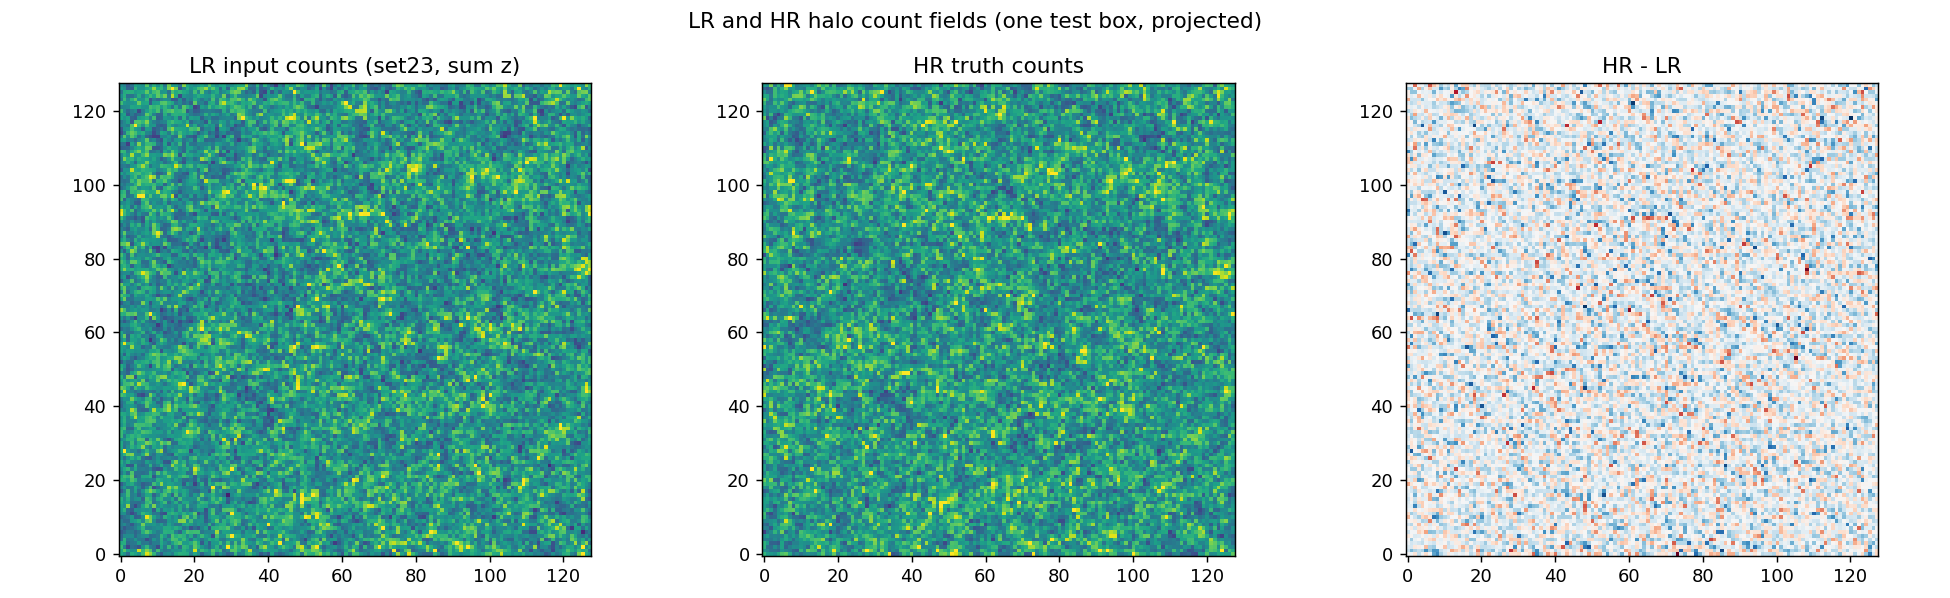
\includegraphics[width=0.9\linewidth]{figures_cmass/data_pair.png}
\caption{One LR/HR pair (projected count map). LR (FastPM, input) and HR
(Quijote N-body, target) share initial conditions and so share large-scale
structure, but differ cell-by-cell.}
\label{fig:srs-datapair}
\end{figure}

\paragraph{Model space (count transform).} The network does not learn on raw
counts; it learns in a compressed ``model space''. The default transform is
$\log(1+n)$, which tames the sparse heavy tail:
\begin{equation}
  y = \log(1+n), \qquad n = \exp(y)-1 \ \ (\text{clamped to } n\ge 0).
  \label{eq:srs-transform}
\end{equation}
Two alternative transforms exist in the code (\texttt{scale}: $n/\text{scale}$;
\texttt{delta}: model space is the overdensity itself), but all reported runs use
$\log(1+n)$. Power spectra are \emph{never} computed in model space; they are
always computed on the physical-count overdensity \SG{Is it okay if this is -1 when there are 0 halos?}
\begin{equation}
  \delta = \frac{n}{\bar n} - 1,
  \label{eq:srs-delta}
\end{equation}
with $\bar n$ the per-box mean count (the \texttt{perbox} setting used in all
runs).

\subsection{Data Pipeline (patching)}
\textit{Located in: \texttt{data/patch\_dataset\_cmass.py},
\texttt{data/patch\_dataset\_real.py} (shared patch ops).}

A model never sees the whole $128^3$ box at once. We cut the box into a
$2\times2\times2$ grid of $64^3$ \textbf{cores} (Table~\ref{tab:srs-notation}).
The cores tile the box exactly (stride $64$), so they reconstruct the box
bit-for-bit with no gaps and no double counting, the dataset's self-test
asserts this. Each model \emph{input} is a core grown by \texttt{pad} voxels on
every side, taken from the true neighbour cells with periodic wrap at the box
edge (\texttt{extract\_patch} uses \texttt{numpy.take(\dots, mode="wrap")}). So
with \texttt{pad}${=}8$ the input is $80^3$ and neighbouring patches overlap by
$2\cdot\texttt{pad}=16$ voxels; the HR \emph{target} is always the bare $64^3$
core. Because each simulation is one continuous periodic box that we crop
ourselves, the patches are real neighbours by construction, there is no data
seam (unlike the Lagrangian patches of \S5). \SG{Isn't the patch construction same in both?}

\begin{table}[t]
\centering
\caption{Notation for the CMASS count-field pipeline.}
\label{tab:srs-notation}
\begin{tabular}{llp{7.2cm}}
\toprule
Symbol & Value & Meaning \\
\midrule
$N_\text{full}$    & $128$ & full box side (voxels) \\
$P$ (\texttt{PATCH}) & $64$ & core side (voxels) \\
$N_\text{patches}$ & $8$ & cores per box ($2{\times}2{\times}2$) \\
\texttt{pad}       & $0$ (Arm A) / $8$ (Arm B) & halo width added to each face by periodic wrap \\
$L_\text{box}$     & $1000\ \mathrm{Mpc}/h$ & box side \\
$\mathbf s$        & $\in\mathbb R^5$ & cosmology vector $(\Omega_m,\Omega_b,h,n_s,\sigma_8)$ \\
$\bar n$           & per-box mean & mean count used to form $\delta=n/\bar n-1$ \\
\bottomrule
\end{tabular}
\end{table}

\begin{figure}[t]
\centering
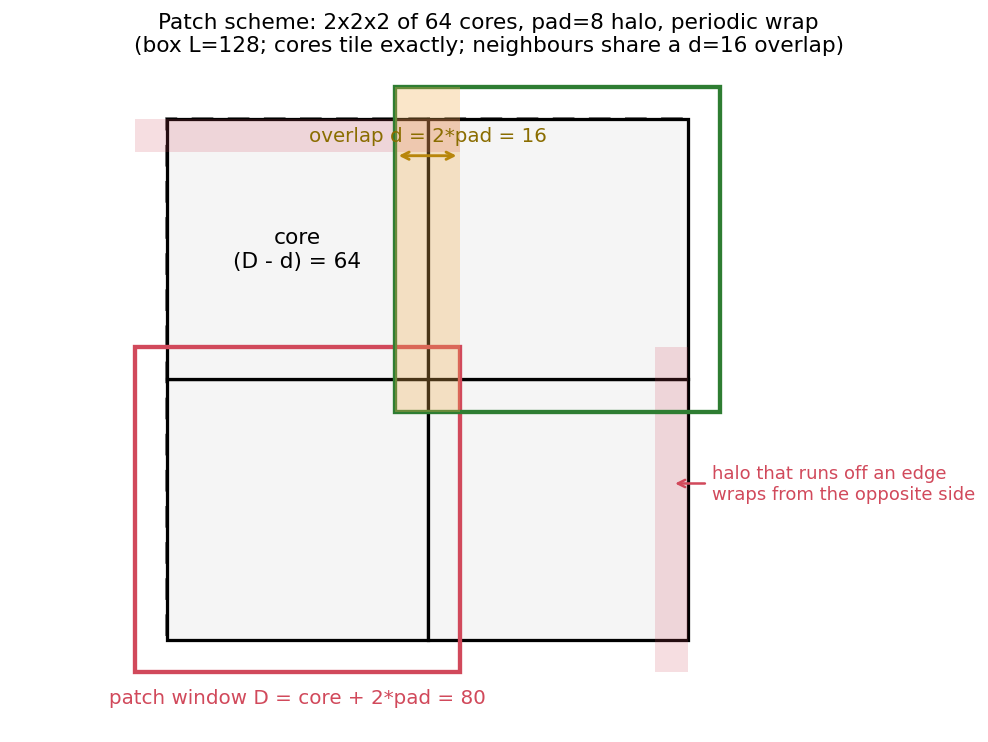
\includegraphics[width=0.82\linewidth]{figures_cmass/pipeline_patching.png}
\caption{Patch scheme. The box is cut into a $2{\times}2{\times}2$ grid of
$64^3$ cores that tile it exactly. With \texttt{pad}${>}0$ each patch is grown by
a halo of real neighbour cells (periodic wrap); only the central core is kept
and placed back.}
\label{fig:srs-patching}
\end{figure}

\paragraph{Per-simulation item.} Indexed by simulation, the dataset returns, for
all $8$ cores at once: the LR patches \texttt{lr\_in} of shape
$(8,\,1,\,64{+}2\,\texttt{pad},\,\cdot,\,\cdot)$ in model space, the HR cores
\texttt{hr\_tgt} of shape $(8,\,1,\,64,\,64,\,64)$, the style $\mathbf s$, and
the simulation index. The trainer flattens the $8$-core axis into the batch.

\begin{algorithm}[H]
\caption{\textsc{ExtractPatches} (one simulation)}
\label{alg:srs-extract}
\begin{algorithmic}[1]
\Require LR box $\mathbf L\in\mathbb R^{1\times128^3}$, HR box $\mathbf H$, \texttt{pad}
\State map $\mathbf L,\mathbf H$ to model space via Eq.~\ref{eq:srs-transform}
\For{$p=0,\dots,7$}
  \State $(i,j,k)\gets\textsc{unravel}(p,(2,2,2))$ \Comment{core origin $(64i,64j,64k)$}
  \State $\mathbf L_p\gets$ core $p$ grown by \texttt{pad} on each face, periodic wrap \Comment{$(64{+}2\,\texttt{pad})^3$}
  \State $\mathbf H_p\gets$ bare core $p$ \Comment{$64^3$}
\EndFor
\State \Return $\{(\mathbf L_p,\mathbf H_p)\}_{p=0}^{7}$, style $\mathbf s$
\end{algorithmic}
\end{algorithm}

\subsection{Model: Input/Output Specification}
\textit{Implementation: \texttt{map2map/models/styled\_srsgan.py}
(\texttt{G\_correct}, \texttt{D\_const}).}

\paragraph{What the generator computes.} The generator is a
\textbf{same-resolution residual} network: it does not change the grid size, and
it predicts a correction that is \emph{added} to the input. In model space,
\begin{equation}
  \mathrm{SR} \;=\; \mathrm{LR} \;+\; G(\mathrm{LR},\,\mathbf s,\,\mathbf z),
  \label{eq:srs-residual}
\end{equation}
where $\mathbf s$ is the cosmology vector and $\mathbf z$ is an injected noise
field (see below). Inputs and outputs are listed in
Table~\ref{tab:srs-model-io}; the generator is run once per core (the $8$ cores
of a box form a batch).

\begin{table}[t]
\centering
\caption{Tensors consumed/produced by the generator \texttt{G\_correct} for one
core (batch dimension omitted). Here $D=64{+}2\,\texttt{pad}$.}
\label{tab:srs-model-io}
\begin{tabular}{lll}
\toprule
Symbol & Shape & Meaning \\
\midrule
$\mathbf x$ (\texttt{x})       & $(1,D,D,D)$ & LR patch, model space (input) \\
$\mathbf s$ (\texttt{style})   & $(5,)$      & cosmology vector \\
$\mathbf z$ (\texttt{noise\_list}) & $2\cdot\texttt{num\_blocks}$ cubes $(1,D,D,D)$ & injected noise; fixed at inference, random in training \\
$G(\cdot)$                     & $(1,D,D,D)$ & predicted residual $\delta$ (added to $\mathbf x$) \\
\bottomrule
\end{tabular}
\end{table}

\paragraph{Internal composition.} $G$ is a constant-resolution StyleGAN2-style
network (no up/down-sampling), built from:
\begin{enumerate}
  \item \texttt{block0}: a $1{\times}1{\times}1$ style-modulated convolution
  (\texttt{ConvStyled3d}) lifting the $1$-channel input to $c_0$ channels,
  followed by a leaky ReLU.
  \item \texttt{num\_blocks} ($=4$) constant-resolution H-blocks
  (\texttt{HBlock\_const}). Each block, in order: inject noise $\to$
  $3{\times}3{\times}3$ \texttt{ConvStyled3d} (periodic ``circular'' padding)
  $\to$ leaky ReLU $\to$ inject noise $\to$ $3{\times}3{\times}3$
  \texttt{ConvStyled3d} $\to$ leaky ReLU $\to$ a $1{\times}1{\times}1$ projection
  to the output channel, accumulated into a running output $y$. The final return
  is $\mathbf x + y$ (Eq.~\ref{eq:srs-residual}).
\end{enumerate}
The channel widths come from \texttt{chan\_base} ($=128$) halved per block and
clamped to $[64,512]$. Two mechanisms make the convolutions depend on side
information:
\begin{itemize}
  \item \textbf{Style modulation.} \texttt{ConvStyled3d} is the StyleGAN2
  modulated/demodulated convolution: the cosmology vector $\mathbf s$ scales the
  convolution weights, so the same network behaves differently for different
  cosmologies. This is the only path by which $\mathbf s$ enters.
  \item \textbf{Noise injection.} Each \texttt{ConvStyled3d} is preceded by a
  per-channel learned-standard-deviation noise add (\texttt{\_NoiseInject}). At
  training time the noise is fresh Gaussian each call; at inference a
  \emph{fixed} list of noise cubes (seeded, built by \texttt{build\_noise\_list})
  is reused so outputs are reproducible. The noise is what lets the model produce
  a plausible small-scale field rather than a single blurred guess.
\end{itemize}

\paragraph{Discriminator.} \texttt{D\_const} is a constant-input-resolution
critic conditioned on the same style $\mathbf s$. It runs a head
\texttt{ConvStyled3d} then \texttt{num\_blocks} strided down-blocks (each a
periodic $3{\times}3{\times}3$ \texttt{ConvStyled3d} $+$ leaky ReLU $+$
$2{\times}$ average pool), a $1{\times}1{\times}1$ tail, and a final
$1{\times}1{\times}1$ projection to one channel, averaged over space to a single
logit per core.

\subsection{Training Step}
\textit{Located in: \texttt{train\_patch\_cmass.py}.}

The generator is trained per core (stitching is \emph{not} part of the
gradient). The total generator loss is a weighted sum of three terms,
\begin{equation}
  \mathcal L_G \;=\; \lambda_\text{adv}\,\mathcal L_\text{adv}
                  + \lambda_\text{rec}\,\mathcal L_\text{rec}
                  + \lambda_\text{pk}\,\mathcal L_\text{pk},
  \label{eq:srs-lossG}
\end{equation}
with (defaults from the original run script; see the protocol update below for
the values now in use):
\begin{itemize}
  \item \textbf{Reconstruction} $\mathcal L_\text{rec}=\lVert \mathrm{SR}-\mathrm{HR}\rVert_1$,
  a plain $L_1$ in model space (optionally Gaussian-smoothed; smoothing off in
  all runs).
  \item \textbf{Power-spectrum} $\mathcal L_\text{pk}$, the mean-squared error
  between the $\log_{10}$ power spectra of SR and HR, computed on the
  \emph{physical-count overdensity} of the $64^3$ core (Eqs.~\ref{eq:srs-transform}--\ref{eq:srs-delta}),
  Hann-windowed, with the HR side detached:
  \begin{equation}
    \mathcal L_\text{pk} = \frac{1}{|K|}\sum_{k\in K}
      \big(\log_{10} P_\text{SR}(k) - \log_{10} P_\text{HR}(k)\big)^2 .
    \label{eq:srs-pkloss}
  \end{equation}
  \item \textbf{Adversarial} $\mathcal L_\text{adv}=\mathrm{softplus}\!\big({-}D(\mathrm{SR},\mathbf s)\big)$,
  the non-saturating GAN generator loss.
\end{itemize}

\paragraph{Protocol update: what region the reconstruction and adversarial
terms see.} A \texttt{--pad-loss} setting controls how much of the generator's
output the $L_1$ and adversarial terms are computed on, independent of
\texttt{pad} itself:
\begin{itemize}
  \item \texttt{crop} (trim-aware, the setting used for Arm B above): the loss
  is computed only on \textsc{cropInterior}$(G(\mathbf x,\mathbf s),\,\texttt{pad})$,
  the $64^3$ core that is actually kept at inference time, against the bare
  $64^3$ HR core. The model is trained on exactly the region it will be graded
  on.
  \item \texttt{full}: the loss is computed on the whole $(64{+}2\,\texttt{pad})^3$
  output, against a correspondingly padded HR target (the dataset's
  \texttt{pad\_target} option). The model is trained as if the halo region it
  will later be trimmed off also mattered.
\end{itemize}
Concretely, let $\texttt{loss\_crop}=\texttt{pad}$ under \texttt{crop} and $0$
under \texttt{full}; every place above that writes $\mathrm{SR}$ means
$\textsc{cropInterior}(G(\mathbf x,\mathbf s),\,\texttt{loss\_crop})$, and the
Hann window and $P(k)$ estimator in $\mathcal L_\text{pk}$ are sized to match.
This is a controlled test of two ways padding could fail to help: see the
protocol-update subsection below for the result.

The discriminator is trained with the non-saturating GAN loss plus a lazy $R_1$
gradient penalty applied every \texttt{r1\_every} steps:
\begin{equation}
  \mathcal L_D = \mathrm{softplus}\!\big({-}D(\mathrm{HR})\big)
               + \mathrm{softplus}\!\big(D(\mathrm{SR})\big)
               + \tfrac{1}{2}\lambda_{R_1}\,\mathbb E\big\lVert \nabla_{\!x} D(x,\mathbf s)\big\rVert^2 .
  \label{eq:srs-lossD}
\end{equation}

\begin{algorithm}[H]
\caption{CMASS patch-GAN training step (one batch of cores)}
\label{alg:srs-train}
\begin{algorithmic}[1]
\Require LR patches $\mathbf x$, HR targets $\mathbf h$ (padded iff \texttt{pad-loss=full}),
         style $\mathbf s$, \texttt{pad}, \texttt{loss\_crop} ($=\texttt{pad}$ if \texttt{crop} else $0$),
         weights $\lambda_\text{adv},\lambda_\text{rec},\lambda_\text{pk},\lambda_{R_1}$
\Statex \textbf{// Discriminator}
\State $\hat{\mathbf h}\gets \textsc{cropInterior}\big(G(\mathbf x,\mathbf s),\,\texttt{loss\_crop}\big)$ \Comment{no grad}
\State $\mathcal L_D \gets \mathrm{softplus}({-}D(\mathbf h,\mathbf s)) + \mathrm{softplus}(D(\hat{\mathbf h},\mathbf s))$
\If{step $\bmod\ \texttt{r1\_every} = 0$} $\mathcal L_D \mathrel{+}= \tfrac12\lambda_{R_1}\texttt{r1\_every}\cdot R_1(D,\mathbf h,\mathbf s)$ \EndIf
\State update $D$ (Adam, grad-clip)
\Statex \textbf{// Generator}
\State $\hat{\mathbf h}\gets \textsc{cropInterior}\big(G(\mathbf x,\mathbf s),\,\texttt{loss\_crop}\big)$
\State $\mathcal L_\text{adv}\gets \mathrm{softplus}({-}D(\hat{\mathbf h},\mathbf s))$
\State $\mathcal L_\text{rec}\gets \lVert \hat{\mathbf h}-\mathbf h\rVert_1$
\State $\mathcal L_\text{pk}\gets$ Eq.~\ref{eq:srs-pkloss} on Hann-windowed overdensity of $\hat{\mathbf h}$, $\mathbf h$
       (skip if $\lambda_\text{pk}{=}0$)
\State $\mathcal L_G \gets \lambda_\text{adv}\mathcal L_\text{adv}+\lambda_\text{rec}\mathcal L_\text{rec}+\lambda_\text{pk}\mathcal L_\text{pk}$
\State update $G$ (Adam, grad-clip)
\end{algorithmic}
\end{algorithm}

\paragraph{Validation and checkpoint selection.} After each epoch we stitch the
full $128^3$ SR box for up to $40$ validation sims and report the stitched
$L_1$/voxel and the stitched-$128$ power-spectrum RMS against HR
(\S\ref{sec:srs-eval}, Eq.~\ref{eq:srs-pkrms}). A \texttt{--select} setting
chooses which of the two the saved \texttt{best.pt} tracks: \texttt{pk} (the
original setting, lowest stitched validation Pk RMS) or \texttt{l1} (lowest
stitched validation $L_1$/voxel). Selection is always on the stitched full box,
not the per-core training loss. Runs that also train with $\lambda_\text{pk}{=}0$
use \texttt{--select l1}, since selecting on Pk RMS while not training on it
would reintroduce the same metric leak in a different place.

\subsection{Inference}
\textit{Located in: \texttt{infer\_stitch\_cmass.py}.}

For one simulation: load the LR $128^3$ count box, map it to model space, run $G$
on each of the $8$ cores (with the periodic-wrap halo in Arm B), crop the halo,
stitch the cores into a $128^3$ model-space box, invert the transform to physical
counts, and clamp. \SG{are all outputs later mapped to integers, or are we fine with non-integer number of halos?} The injected noise list is fixed (seeded) so the output is
reproducible.

\begin{algorithm}[H]
\caption{CMASS inference + stitch (one simulation)}
\label{alg:srs-infer}
\begin{algorithmic}[1]
\Require LR box $\mathbf L$, style $\mathbf s$, trained $G$, mode (naive/overlap), fixed noise $\mathbf z$
\State $\texttt{pad}\gets 0$ if naive else value from checkpoint ($8$)
\State map $\mathbf L$ to model space (Eq.~\ref{eq:srs-transform})
\For{$p=0,\dots,7$}
  \State $\mathbf x_p\gets$ patch $p$ (core grown by \texttt{pad}, periodic wrap)
  \State $\mathbf c_p\gets \textsc{cropInterior}\big(G(\mathbf x_p,\mathbf s,\mathbf z),\,\texttt{pad}\big)$ \Comment{$64^3$ core, model space}
\EndFor
\State $\mathbf S\gets \textsc{stitch}(\{\mathbf c_p\})$ \Comment{$128^3$, model space}
\State $\mathbf S\gets \exp(\mathbf S)-1$, clamp to $[0,\,C_\text{max}{=}200]$, replace NaN/Inf \Comment{physical counts}
\State \Return $\mathbf S$
\end{algorithmic}
\end{algorithm}

\subsection{Crop Stitching}

Stitching is \textbf{direct placement with no averaging}. Adjacent cores tile the
box exactly (stride $64$, no overlap between cores once the halo is dropped), so
each core's $64^3$ output is written straight into its slot. In Arm B the $80^3$
patch is corrected and only its central $64^3$ core is kept; the overlap halo is
context for the convolution, never written to the output.

\begin{algorithm}[H]
\caption{\textsc{Stitch} ($8$ cores $\to$ $128^3$)}
\label{alg:srs-stitch}
\begin{algorithmic}[1]
\Require cores $\{\mathbf c_p\}_{p=0}^{7}$, each $1\times64^3$
\State $\mathbf S\gets \mathbf 0\in\mathbb R^{1\times128^3}$
\For{$p=0,\dots,7$}
  \State $(i,j,k)\gets\textsc{unravel}(p,(2,2,2))$
  \State $\mathbf S[:,\,64i{:}64i{+}64,\,64j{:}\cdots,\,64k{:}\cdots]\gets \mathbf c_p$ \Comment{direct assignment}
\EndFor
\State \Return $\mathbf S$
\end{algorithmic}
\end{algorithm}

\subsection{Evaluation}
\label{sec:srs-eval}
\textit{Located in: \texttt{analysis/eval\_seam\_cmass.py},
\texttt{analysis/diag\_cmass.py}, \texttt{analysis/match\_stats\_cmass.py},
\texttt{analysis/power\_spectrum.py}, \texttt{inference/nde.py},
\texttt{evaluate.py}.}

We evaluate the SR field against HR at three levels: a seam check (does stitching
leave a join?), field statistics (does SR have the right structure?), and
cosmology (does SR give the same parameter posterior as HR?).

\paragraph{Power-spectrum summaries.} On the count overdensity (Eq.~\ref{eq:srs-delta})
we report the power spectrum $P(k)$, the transfer ratio, and the cross-coherence:
\begin{equation}
  T(k) = \frac{P_\text{SR}(k)}{P_\text{HR}(k)},
  \qquad
  r(k) = \frac{P_{\text{SR},\text{HR}}(k)}{\sqrt{P_\text{SR}(k)\,P_\text{HR}(k)}} .
  \label{eq:srs-Tr}
\end{equation}
$T(k)=1$ means SR has the right \emph{amount} of power at scale $k$ (amplitude);
$r(k)=1$ means SR has the structure in the right \emph{place} (phase). The
scalar power-spectrum error used for checkpoint selection and seam reporting is
the log-RMS over the resolved $k$-bins:
\begin{equation}
  \mathrm{PkRMS}_{\log_{10}} = \sqrt{\frac{1}{|K|}\sum_{k\in K}
    \big(\log_{10} P_\text{SR}(k) - \log_{10} P_\text{HR}(k)\big)^2 } .
  \label{eq:srs-pkrms}
\end{equation}

\paragraph{Seam diagnostic.} \texttt{eval\_seam\_cmass.py} bins the per-cell
count error $|{\mathrm{SR}-\mathrm{HR}}|$ by distance to the nearest core face
and forms a per-position error profile along each axis. The headline number is
the \textbf{$x{=}64$ internal-seam excess}: the error on the internal core
boundary plane divided by the interior error. A value near $1$ means stitching
leaves no seam. The box edge $x{=}0$ is a periodic-boundary control.

\paragraph{Field-match statistics.} \texttt{match\_stats\_cmass.py} reports, over
$16$ test boxes: the total-count ratio $\sum\mathrm{SR}/\sum\mathrm{HR}$, the
void fraction (cells $<0.5$), the real-space cell standard-deviation ratio
$\mathrm{std}(\mathrm{SR})/\mathrm{std}(\mathrm{HR})$ (a blur check), and the
cross-coherence $r(k)$ at large ($k<0.05$) and small ($k>0.2$) scales.

\paragraph{Cosmology (posterior consistency).} This is the strongest ``does SR
match HR'' test. We voxel-count $\to$ overdensity $\to$ $P(k)$ for every box, then
train a neural density estimator $q(\theta\mid P(k))$ on the training split using
\texttt{sbi} (\texttt{SNPE\_C} with a neural-spline-flow density estimator,
\texttt{inference/nde.py}); the summary is $\log_{10}P(k)$. We train one estimator
on HR ($q_\text{HR}$) and one on each SR arm ($q_\text{SR}$). For each test box we
draw $2000$ posterior samples from each, fit a Gaussian per parameter, and report
the per-parameter Gaussian KL (\texttt{evaluate.py}):
\begin{equation}
  \mathrm{KL}\big(\mathcal N(\mu_\text{HR},\sigma_\text{HR})\,\Vert\,\mathcal N(\mu_\text{SR},\sigma_\text{SR})\big)
  = \tfrac12\!\left[\log\frac{\sigma_\text{SR}^2}{\sigma_\text{HR}^2}
    + \frac{\sigma_\text{HR}^2+(\mu_\text{HR}-\mu_\text{SR})^2}{\sigma_\text{SR}^2} - 1\right].
  \label{eq:srs-kl}
\end{equation}
$\mathrm{KL}=0$ means SR gives the identical cosmology posterior to HR. The raw LR
field (no model), pushed through the same pipeline, is the control SR must beat.

We report this comparison in two forms, and it matters which is which:
\begin{itemize}
  \item \textbf{Cross-fidelity (primary).} $q_\text{SR}$ is trained on SR power
  spectra but \emph{evaluated on the HR} $P(k)$ of each test simulation, and
  compared to $q_\text{HR}$ evaluated on the same HR $P(k)$. This is the
  deployment scenario the project targets: HR simulations are too expensive to
  train an inference model on, so the inference model is trained on cheap SR
  output and must still work when applied to (HR-like) reality. The comparison
  against an LR-trained estimator on the same HR data measures whether sampling
  in HR space (SR) survives the distribution shift better than staying in LR
  space. This metric never appears in the training loss.
  \item \textbf{Own-data (secondary).} $q_\text{SR}$ trained and evaluated on SR
  vs $q_\text{HR}$ trained and evaluated on HR, each pipeline end-to-end on
  its own field type.
\end{itemize}

\subsection{Best-Run Configuration}
\textit{Run script: \texttt{scripts/train\_patch\_cmass.slurm}; checkpoints
\texttt{checkpoints/patch\_cmass\_\{A,B\}/best.pt}.}

Both arms use the identical configuration below; they differ only in \texttt{pad}
($0$ for Arm~A, $8$ for Arm~B). This is the configuration behind every number
in \S\ref{sec:srs-results}--\S\ref{sec:srs-next}.

\begin{lstlisting}[language=bash]
--transform log1p   --nbar perbox        # log(1+n) model space; per-box nbar
--epochs 30         --sims-per-batch 1    # patch-batch = 8 cores per step
--chan-base-g 128   --chan-base-d 64  --num-blocks 4
--lambda-adv 1.0    --lambda-rec 2.0  --lambda-pk 2.0   # generator weights
--lambda-r1 10.0    --r1-every 16                       # lazy R1
--lr-g 1e-4 --lr-d 1e-4  --beta1 0.0 --beta2 0.99       # Adam
--grad-clip 1.0     --val-max-sims 40    --select pk    # select on Pk RMS
\end{lstlisting}

The best checkpoint per arm is the one with the lowest stitched validation Pk RMS
(Eq.~\ref{eq:srs-pkrms}):

\begin{center}
\begin{tabular}{lc}
\toprule
arm & best stitched val PkRMS$_{\log_{10}}$ \\
\midrule
Arm A, naive (pad $0$)  & $0.0947$ \\
Arm B, overlap (pad $8$) & $0.0963$ \\
\bottomrule
\end{tabular}
\end{center}

\paragraph{Protocol update.} Following the mentor meeting reported in
\S\ref{sec:srs-followup}, the configuration above is no longer the one we train
with. Three settings changed:
\begin{lstlisting}[language=bash]
--lambda-pk 0.0      # power-spectrum term OFF (it was also our main metric)
--pad-loss crop|full # trim-aware vs trim-unaware padding, see below
--select l1          # select on stitched L1, not the term we removed
\end{lstlisting}
All results in \S\ref{sec:srs-followup} use this configuration. Runs under the
original configuration above (Arm A, Arm B, and everything derived from them in
\S\ref{sec:srs-results}--\S\ref{sec:srs-next}) remain valid as a record of that
protocol; they are superseded, not invalidated, by the update.

\subsection{Results: Does SR Match HR?}
\label{sec:srs-results}

All numbers are on the $200$-box test split unless noted.

\paragraph{1. Power spectrum (statistics).} Across the test set the SR power
spectrum tracks HR at every scale, and Arm A beats the no-model LR control on the
overall log-RMS (Fig.~\ref{fig:srs-srvshr}, computed by
\texttt{analysis/plot\_sr\_vs\_hr.py}).

\begin{table}[h]
\centering
\caption{SR vs HR power-spectrum agreement, $200$ test boxes. Transfer
$T(k)=P_X/P_\text{HR}$ (Eq.~\ref{eq:srs-Tr}); $1.0$ is perfect.}
\label{tab:srs-pk}
\begin{tabular}{lccc}
\toprule
field (vs HR) & PkRMS$_{\log_{10}}$ & $T$ at large scales ($k{<}0.1$) & $T$ at small scales ($k{>}0.3$) \\
\midrule
SR (Arm A, naive)    & $\mathbf{0.0607}$ & $0.95$ & $1.04$ \\
SR (Arm B, overlap)  & $0.0645$ & $0.93$ & $0.88$ \\
LR (no model, control) & $0.0641$ & $1.01$ & $1.01$ \\
\bottomrule
\end{tabular}
\end{table}

\begin{figure}[t]
\centering
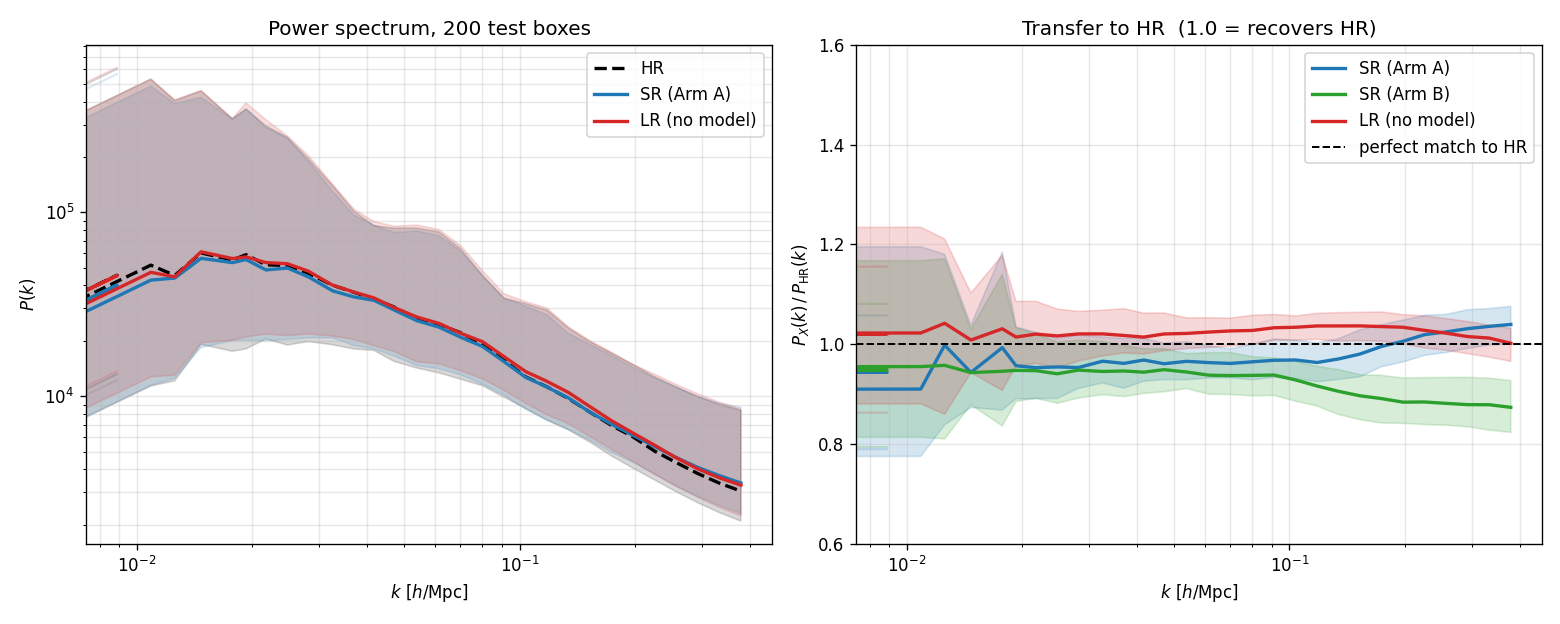
\includegraphics[width=0.98\linewidth]{figures_cmass/sr_vs_hr_pk.png}
\caption{\textbf{Left:} $P(k)$ of HR, SR (Arm A), and LR over $200$ test boxes
(median $+$ $16/84\%$ band). \textbf{Right:} transfer to HR; $1.0$ recovers HR.
SR (Arm A) sits near $1$ at all scales; Arm B's overlap blending slightly
suppresses small-scale power (transfer $0.88$).}
\label{fig:srs-srvshr}
\end{figure}

\paragraph{2. Field structure.} Beyond the power spectrum, SR keeps the field
structure of HR (Arm A, $16$ test boxes, \texttt{match\_stats\_cmassA.txt}):

\begin{table}[h]
\centering
\caption{SR vs HR field-match statistics (Arm A).}
\label{tab:srs-match}
\begin{tabular}{lll}
\toprule
quantity & value & reading \\
\midrule
total count ratio $\sum\mathrm{SR}/\sum\mathrm{HR}$ & $0.965\pm0.172$ & counts conserved on average; large per-box scatter \\
real-space std ratio & $1.008\pm0.100$ & clustering amplitude matches; not blurred \\
void fraction SR / HR ($<0.5$) & $0.855$ / $0.833$ & SR keeps voids empty, like HR \\
cross-coherence $r$, $k<0.05$ & $0.951$ & large-scale structure matches cell-by-cell \\
cross-coherence $r$, $k>0.2$ & $0.403$ & small-scale structure decorrelates \\
\bottomrule
\end{tabular}
\end{table}

\paragraph{3. Cosmology.} The cosmology comparison in the original report used
mislabeled cosmologies, an indexing bug we describe and fix in
\S\ref{sec:srs-correction}, so those numbers are not shown here. With correct
labels a single box constrains $\Omega_m$ and $\sigma_8$; at the power spectrum
level the raw LR field is already HR-like, while at the field level an SR-trained
posterior transfers to HR and an LR-trained one does not
(\S\ref{sec:srs-correction}, Table~\ref{tab:srs-corrected}).

\paragraph{4. Seam.} Neither arm introduces a stitching seam: the $x{=}64$
internal-seam excess is $\approx1$ for both
(Table~\ref{tab:srs-seam}, Fig.~\ref{fig:srs-seam}). Arm A shows a mild generic
ripple near \emph{any} boundary plane (seam-distance ratio $1.17$); Arm B's
overlap removes it ($1.00$) at a small cost in Pk RMS.

\begin{table}[h]
\centering
\caption{Seam and stitched-fidelity metrics, $200$ test boxes. ``Excess'' is
boundary error over interior error; $\approx1$ means no seam.}
\label{tab:srs-seam}
\begin{tabular}{lccp{5.2cm}}
\toprule
metric & Arm A naive & Arm B overlap & reading \\
\midrule
$x{=}64$ internal-seam excess & $0.9934$ & $0.9998$ & no internal seam either arm \\
seam-distance ratio ($d{=}0/d{\ge}8$) & $1.1729$ & $1.0032$ & generic boundary ripple, removed by overlap \\
$x{=}0$ periodic edge (control) & $0.9930$ & $0.9993$ & box edge behaves like interior \\
stitched PkRMS$_{\log_{10}}$ vs HR & $0.0637$ & $0.0678$ & stitched power-spectrum match \\
\bottomrule
\end{tabular}
\end{table}

\begin{figure}[t]
\centering
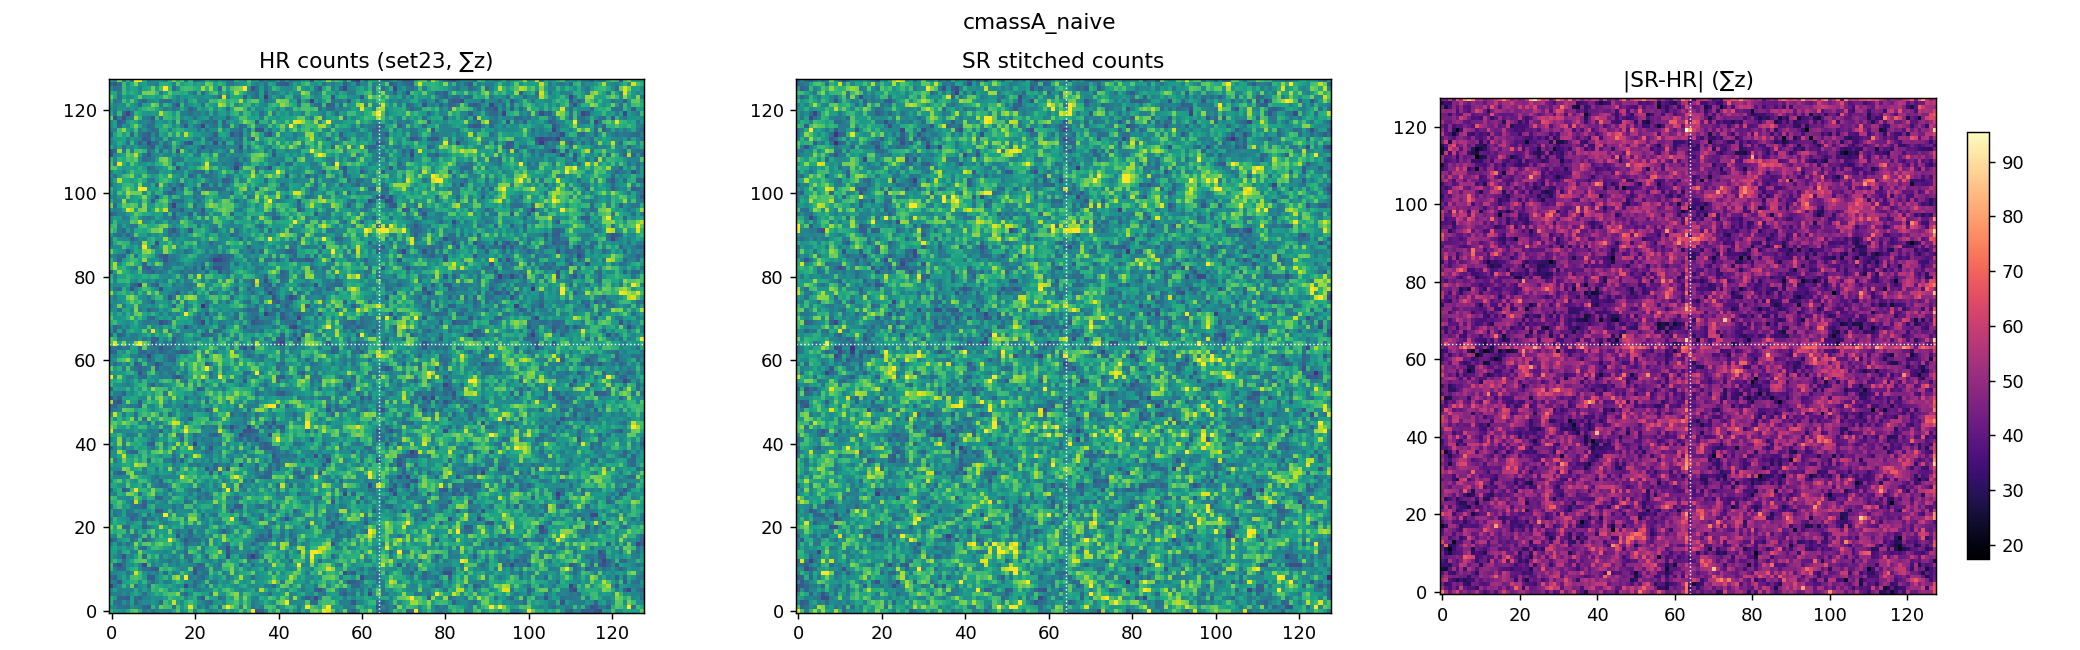
\includegraphics[width=0.95\linewidth]{figures_cmass/seam_cmassA_naive_slice.png}
\caption{Projected count maps for one test box (Arm A): HR, stitched SR, and the
absolute residual $|\mathrm{SR}-\mathrm{HR}|$. White dotted lines mark the
$x{=}64$, $y{=}64$ core boundaries; the residual shows no elevated ridge along
them.}
\label{fig:srs-seam}
\end{figure}

\paragraph{Per-scale diagnostic panels.} Figure~\ref{fig:srs-pkpanel} shows the
full-box $P(k)$, transfer, and cross-coherence for Arm A. The transfer sits near
$1$ at all scales (right amount of power); the cross-coherence is near $1$ at
large scales and falls toward small scales (structure placement is recovered at
large scales only). The per-patch panel
(\texttt{figures\_cmass/pk\_panel\_patch\_cmassAfix.png}) and the projection panels
(\texttt{projection\_box\_cmassAfix\_set23.png},
\texttt{projection\_patch\_cmassAfix\_set23\_p0.png}) tell the same story; Arm~B's
panels carry the \texttt{cmassB} suffix.

\begin{figure}[t]
\centering
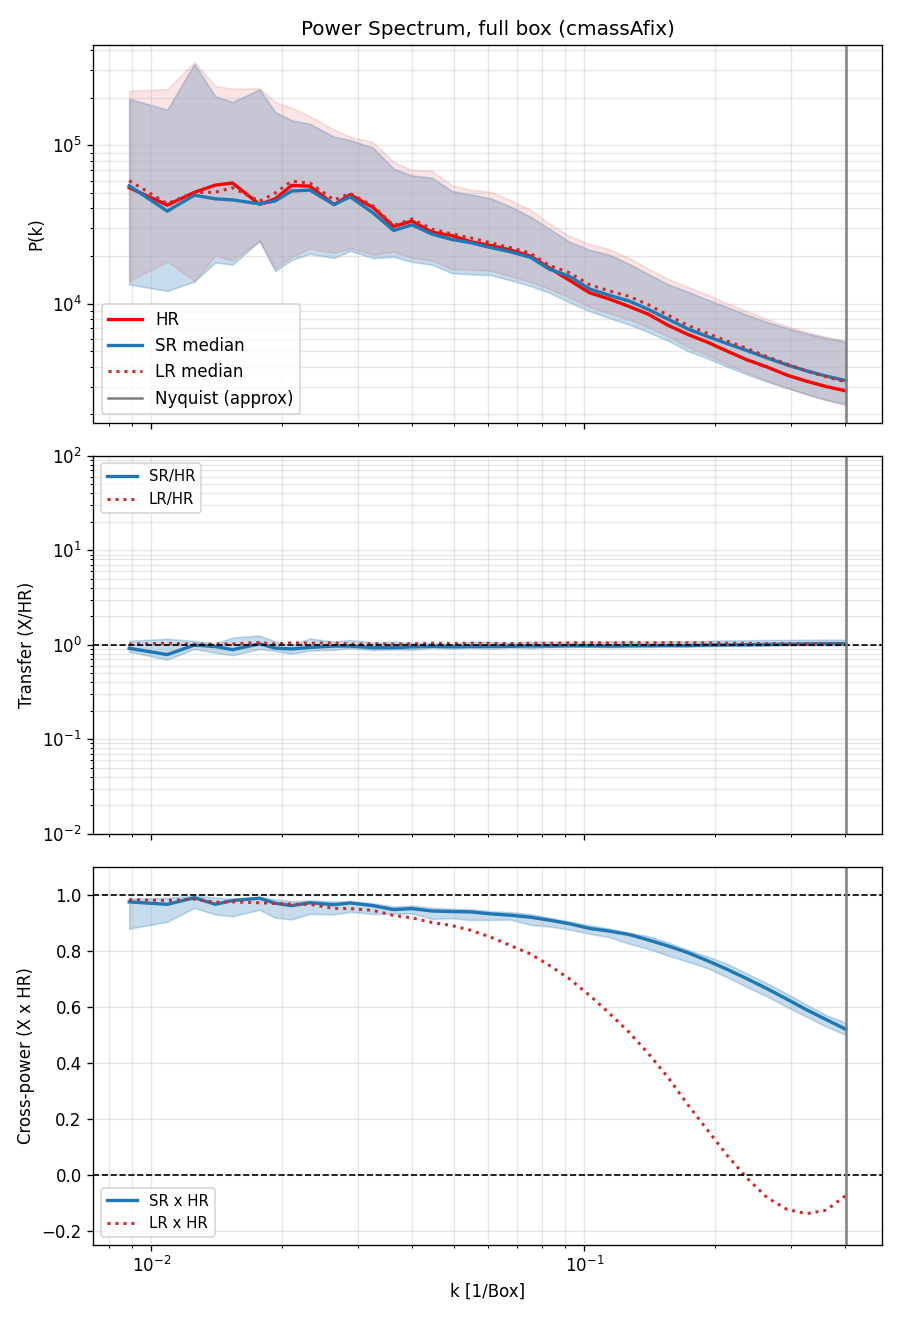
\includegraphics[width=0.5\linewidth]{figures_cmass/pk_panel_box_cmassAfix.png}
\caption{Full-box diagnostic for the conditioned generator (fiducial cosmology,
$16$ test boxes): $P(k)$ of HR (red), SR (blue median $+$ band), and LR (dotted
red); transfer $T(k)=P_X/P_\text{HR}$ on a linear axis with the 16 to 84
percentile band for both SR and LR, the legend reporting the RMS deviation of
each ratio from unity; and cross-coherence $r(k)$. The SR median transfer sits
below unity for $k<0.1$, a systematic large-scale power deficit of roughly 5 to
10 percent, while LR sits slightly above unity; SR does not tighten the transfer
scatter relative to LR. In $r(k)$, SR stays near unity to smaller scales while
LR decorrelates.}
\label{fig:srs-pkpanel}
\end{figure}

\subsection{Diagnostic: What is NOT Working}

\paragraph{Small-scale structure decorrelates, and this is fundamental.} SR
matches HR cell-by-cell at large scales ($r{=}0.95$ for $k<0.05$) but loses the
match at small scales ($r{=}0.40$ for $k>0.2$, Table~\ref{tab:srs-match}). This
is not a capacity bug: it is set by how much information the LR input carries
about HR. LR and HR share large-scale modes but the voxel-by-voxel LR$\leftrightarrow$HR
correlation is only $\approx0.06$, so the exact small-scale realization is simply
not present in the input. The model can match the small-scale \emph{statistics}
(transfer $\approx1$, real-space std ratio $1.008$) but cannot reproduce the
exact placement of individual halos. The noise injection
(Eq.~\ref{eq:srs-residual}) exists precisely because of this: it draws a
plausible small-scale field rather than regressing to a blur.

\paragraph{Per-box total-count scatter.} The total halo count is conserved on
average but with $\sim17\%$ per-box scatter ($\sum\mathrm{SR}/\sum\mathrm{HR}=
0.965\pm0.172$). A count-aware output head (predict a rate and sample Poisson
counts) would tighten this; it is the one clearly addressable imperfection. \SG{I would think this isn't necessary to fix, we don't care about the number of halos after all.}

\paragraph{Overlap suppresses small-scale power.} Arm B's overlap blending lowers
the small-scale transfer to $0.88$ (Table~\ref{tab:srs-pk}), so on the power
spectrum the naive Arm A is the better super-resolver. Overlap removes a small
generic boundary ripple but buys no fidelity, because on this continuous count
data there is no real seam to fix, the clean version of the mentor 2.1 vs 2.2
comparison.

\paragraph{Where the cosmology value is.} At the power spectrum level the raw LR
field is already close to HR, since they share large-scale modes, so the power
spectrum is a forgiving summary with little headroom. The model's value is at the
field level (variance, voids, small-scale structure), which the power spectrum
summary is insensitive to. The corrected cross-fidelity in
\S\ref{sec:srs-correction} bears this out: SR and LR are indistinguishable at the
power spectrum level, but at the field level an SR-trained posterior transfers to
HR while an LR-trained one does not.

\subsection{What I'm Trying Next}
\label{sec:srs-next}

The diagnostics above point to one limit that may be fundamental (small-scale
decorrelation) and a few that are clearly fixable (count scatter, small-scale
realism). The plan below is ordered so that we \emph{measure} the limit before
spending effort trying to beat it. None of these results are in yet; this is the
roadmap, not an experiment log.

\paragraph{Step 0, measure the information ceiling first.} Before trying to
improve the small-scale match, we need to know whether $r{=}0.40$ at small scales
(Table~\ref{tab:srs-match}) is the best any model could do from this input, or a
weakness of the current one. Two cheap diagnostics settle it:
\begin{itemize}
  \item \textbf{LR$\leftrightarrow$HR cross-coherence $r_\text{LR,HR}(k)$.} The
  cross-coherence of the \emph{raw input} against HR (no model) is the ceiling:
  no function of LR can place small-scale structure better than the input
  already correlates with HR. If $r_\text{SR,HR}(k)\approx r_\text{LR,HR}(k)$ at
  small $k$, the model is already at the ceiling and the limit is fundamental;
  if it sits well below, there is recoverable structure left on the table. (Only
  per-box $P(k)$ is currently saved, not the cross-spectrum, so this needs one
  re-run that keeps the fields.)
  \item \textbf{No-noise ablation.} Train the same generator with the noise
  injection off (a plain regressor). Theory predicts this should \emph{raise} the
  small-scale cross-coherence a little (a regressor targets the conditional mean,
  the best cell-by-cell predictor) but \emph{lower} the small-scale transfer well
  below $1$ (the conditional mean is blurry). Seeing exactly that trade-off would
  confirm that the noise/GAN is the right choice for a power-spectrum target, and
  would quantify how much cell-by-cell accuracy is being traded for correct
  statistics.
\end{itemize}

\paragraph{Step 1, fix the count scatter and small-scale realism (independent
of the ceiling).} These help regardless of what Step 0 finds:
\begin{itemize}
  \item \textbf{Count-aware (Poisson) output head.} Instead of predicting a
  count directly, predict a non-negative rate $\lambda$ per cell and sample the
  count as $n\sim\mathrm{Poisson}(\lambda)$. Halo counts are discrete and sparse,
  so a Poisson head models the small-scale graininess as actual shot noise rather
  than a smeared residual, and should tighten the $\sim17\%$ per-box total-count
  scatter (Table~\ref{tab:srs-match}), the one clearly addressable imperfection.
  \item \textbf{Explicit statistics terms in the loss.} Add a one-point PDF /
  variance matching term so small-scale sharpness is enforced directly, rather
  than relying on the adversarial term alone to find it.
  \item \textbf{Loss rebalance.} The current weights are $\lambda_\text{rec}{=}2$,
  $\lambda_\text{pk}{=}2$, $\lambda_\text{adv}{=}1$
  (Eq.~\ref{eq:srs-lossG}). The $L_1$ term blurs; lowering it and raising the
  adversarial weight should push toward correct statistics, at a known cost in
  cell-by-cell accuracy, per the same trade-off as the no-noise ablation.
\end{itemize}

\paragraph{Step 2, extract more of the available information (only if Step 0
shows headroom).} If $r_\text{SR,HR}$ sits below the LR$\leftrightarrow$HR
ceiling, the model is under-using its input. A larger receptive field, or feeding
each patch more neighbour context, would let it use more of the LR field to
predict the residual. This only helps if there is headroom to recover.

\paragraph{Step 3, raise the ceiling by changing the \emph{input}, not the
model.} The small-scale cell-by-cell limit is set by the information in the LR
input (the voxel-by-voxel LR$\leftrightarrow$HR correlation is only
$\approx0.06$). No amount of model capacity raises that; only more informative
inputs do. Candidates: feed the shared small-scale \emph{initial conditions}
(which the coarse LR count field has discarded), or add the LR velocity / particle
fields. This is the only route to a meaningful gain in small-scale cross-coherence,
and is the natural bridge to the displacement-field model of \S5, which already
carries that extra information.

\paragraph{Summary.} Steps 0--1 are the near-term plan: measure the ceiling, then
add a Poisson head and statistics losses to fix the count scatter and sharpen the
small-scale field. Steps 2--3 are contingent on what Step 0 reveals. For a
cosmology deliverable the priority is statistical fidelity (which Steps 0--1
target); exact small-scale reconstruction (Step 3) is a larger, input-level
change worth it only if cell-by-cell recovery becomes the goal.

\subsection{Follow-Up Results: New Protocol from the Mentor Meeting}
\label{sec:srs-followup}

A mentor meeting after the report above changed two things about how we train
and evaluate this model. First, the real goal is not to match HR with SR by
itself. The real goal is to train a posterior model on SR output and have it
work well when it is tested on real HR data, since HR simulations are too
expensive to train a posterior model on directly. Second, the power spectrum
term was removed from the training loss, since it was also our main success
metric and that is a weak test. This subsection reports what we found. Some of
the training runs below are still in progress at the time of writing, so
numbers marked as current are read from the latest completed epoch, not a
final result.

\paragraph{Held-out check: the bispectrum.} A fair worry is that our power
spectrum result looks good only because the power spectrum was also in the
training loss. To check this we measured the bispectrum, a higher-order
statistic that was never used anywhere in training or model selection. If SR
only matches the power spectrum and nothing else, the bispectrum should show
no improvement over the raw LR input.

\begin{figure}[t]
\centering
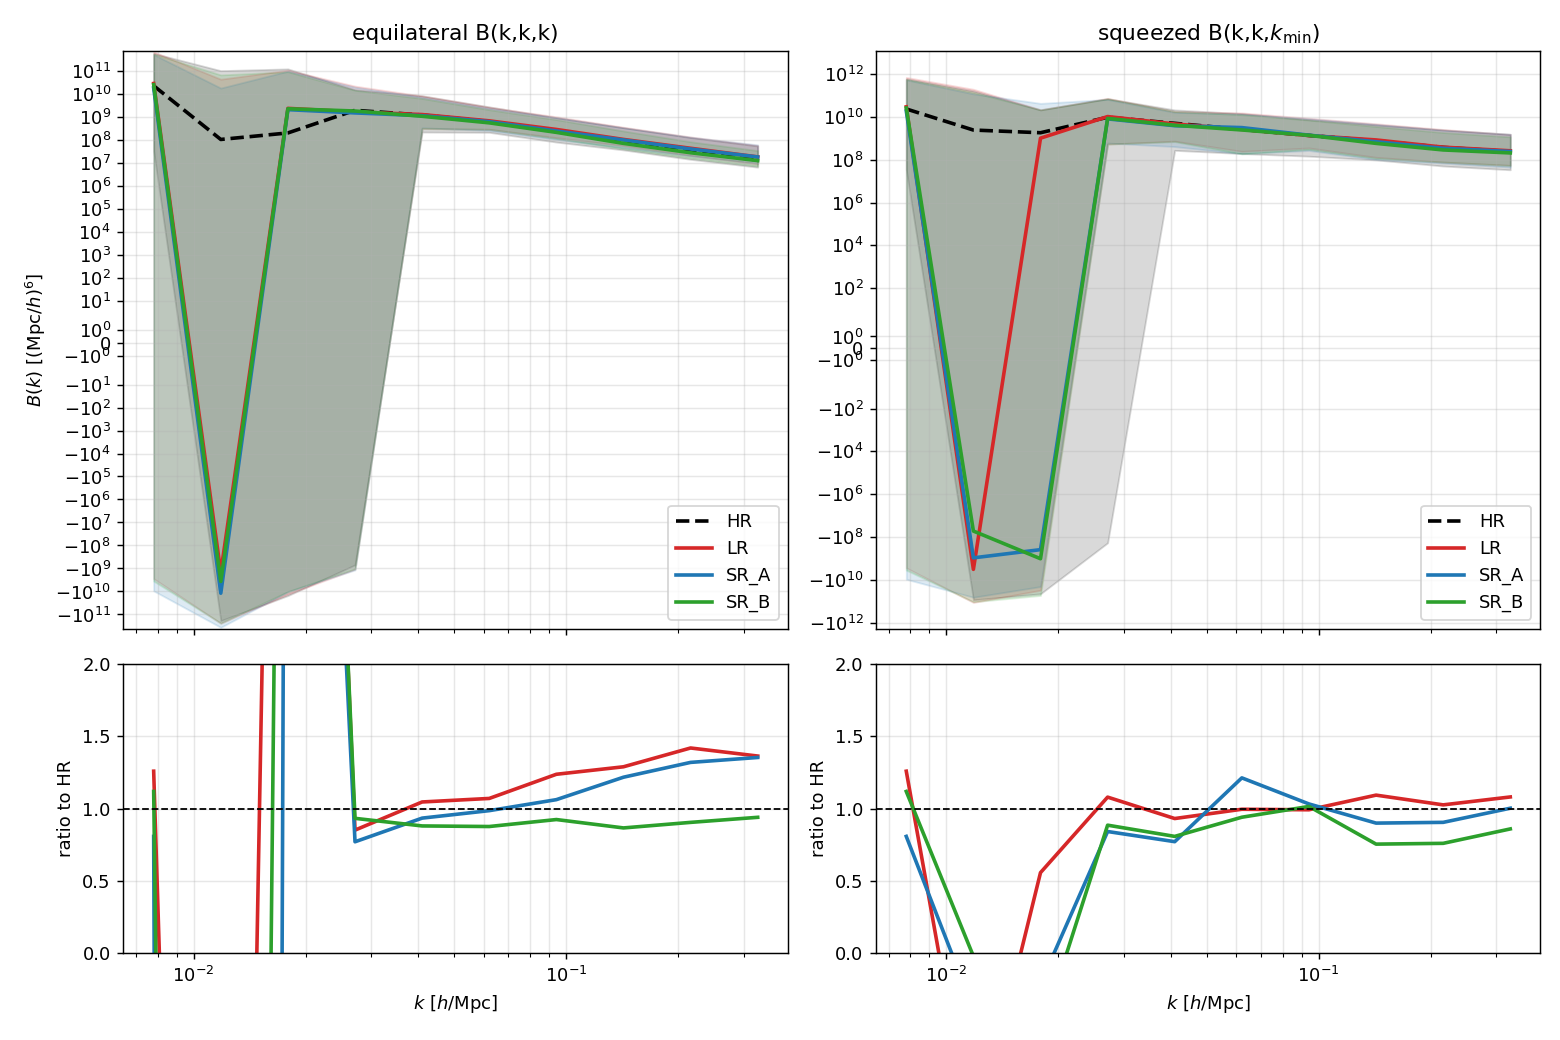
\includegraphics[width=0.95\linewidth]{figures_cmass/bispectrum_hr_lr_srA_srB.png}
\caption{Bispectrum of HR, LR, and SR (both arms), on $16$ test boxes. Top:
equilateral and squeezed bispectrum, HR in black. Bottom: ratio to HR. SR
removes most of the systematic excess that LR has at the plotted scales,
without ever training on this statistic.}
\label{fig:srs-bispec}
\end{figure}

On the equilateral configuration, LR sits about $6$ to $13$ percent above HR
across the middle range of scales. SR removes most of this gap without ever
seeing a bispectrum during training, and it does this for both arms. This is
evidence that the model is not simply fitting the training metric. It is
correcting real structure in the field that also shows up in a statistic it
never saw. (The figure uses the earlier models trained \emph{with} the power
spectrum loss; the no-Pk models of the following paragraphs preserve the
bispectrum at least as well, so removing that loss did not degrade this
held-out statistic either.)

\paragraph{Removing the power spectrum loss.} Following the meeting, we
retrained the model with the power spectrum term switched off
($\lambda_\text{pk}{=}0$ in Eq.~\ref{eq:srs-lossG}), so the loss is only the
adversarial and $L_1$ terms. We also changed which checkpoint counts as "best"
to the real-space $L_1$ error, since selecting on the power spectrum would
have been the same kind of leak we were trying to remove.

\begin{figure}[t]
\centering
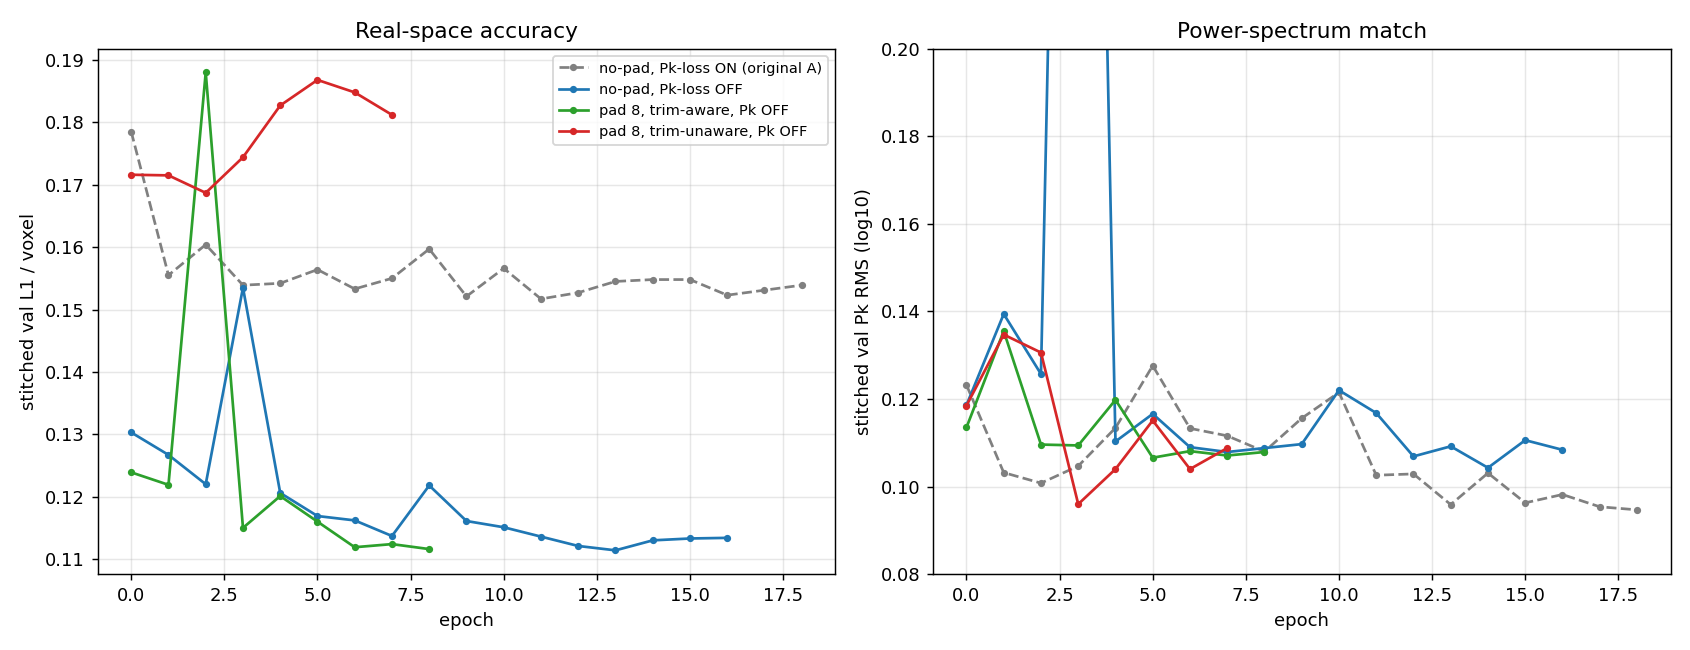
\includegraphics[width=0.98\linewidth]{figures_cmass/protocolv2_cmass.png}
\caption{Stitched validation curves under the new protocol (power spectrum
loss off). Left: real-space $L_1$ error. Right: power spectrum RMS error. Grey
dashed: the original Arm A with the power spectrum loss on, for comparison.
These runs are still training; curves stop at the most recent completed
epoch.}
\label{fig:srs-protocolv2}
\end{figure}

Two things stand out so far. First, without the power spectrum term, the
real-space $L_1$ error becomes clearly better than the original run at the
same point in training (left panel, blue and green curves sit below the grey
dashed curve). Second, the power spectrum error does get a little worse
without its loss term, but it does not collapse: it settles into roughly the
same range as before, just a bit noisier. So the power spectrum term was
buying us a small amount of power spectrum accuracy at a real cost in
real-space accuracy. It was not the only reason the power spectrum matched
well; the adversarial and reconstruction terms carry most of that on their
own.

\paragraph{Does padding help, once the power spectrum loss is out of the way?}
The report above found that padding (Arm B) did not beat no padding (Arm A) on
the power spectrum. The mentor pointed out two different ways this could
happen, and that they make different, testable predictions:
\begin{itemize}
  \item \textbf{Trim-aware.} The model is trained knowing that only the middle
  part of its output will be kept; the loss only looks at that middle part.
  This is what Arm B already did. If this is working correctly, padding should
  train at least as well as no padding, since it has strictly more context for
  the same target.
  \item \textbf{Trim-unaware.} The model is trained as if its whole padded
  output matters, including the edge region that gets thrown away later. If
  the model leans on that edge region during training, it should look fine
  during training but generalize worse once the edge is cut off at test time.
\end{itemize}
We trained both versions with the power spectrum loss off, so the comparison
is not confused by that term. Figure~\ref{fig:srs-protocolv2} shows all three
runs together (no padding, trim-aware padding, trim-unaware padding).

The trim-aware version (green) matches or beats no-padding (blue) on both
real-space error and power spectrum error at almost every epoch measured so
far. This supports the first prediction: once the model is told correctly what
part of its output is graded, more context helps rather than hurts. The
trim-unaware version (red) is clearly worse on real-space error than both
other runs, and does not close that gap as training continues. This supports
the second prediction: a model that is allowed to rely on the part of its
output that gets discarded at test time pays for that at test time. Put
together, the original result that padding did not help was most likely
caused by the power spectrum loss, not by padding itself.

We also reran the older, padding-with-power-spectrum-loss model for more
epochs to check whether it had simply not been trained long enough. Fifteen
additional epochs did not beat its early best score, so that run was not
undertrained; the training recipe, not the training time, was the limiting
factor.

\subsection{The Goal Metric: Corrected Cross-Fidelity Results}
\label{sec:srs-correction}

\paragraph{The bug.} After the analysis above, a routine physical sanity check
failed in a way that could not be real: the amplitude of the power spectrum had
essentially zero correlation with $\sigma_8$, and a fit of the power spectrum to
the five parameters explained only $0.2\%$ of the variance. The power spectrum
amplitude must scale with $\sigma_8$, so this pointed to a labeling error, not to
physics. Tracing it, we found that the processed count fields were written in
string-sorted simulation order ($0, 1, 10, 100, 1000, \dots$) while the cosmology
table is indexed numerically. Field number $k$ is therefore the halo field of
simulation string-sort$(k)$, not simulation $k$, so every field in the whole
pipeline was paired with the wrong cosmology. We proved this exactly: using the
original halo catalogs, the field halo count matches the catalog count under the
string-sort permutation for all $2000$ simulations, while the identity mapping
matches only the two fixed points. We corrected the cosmology table to field
order, backed up the old one, and patched the builder so it cannot regenerate the
wrong order.

\begin{figure}[h]
\centering
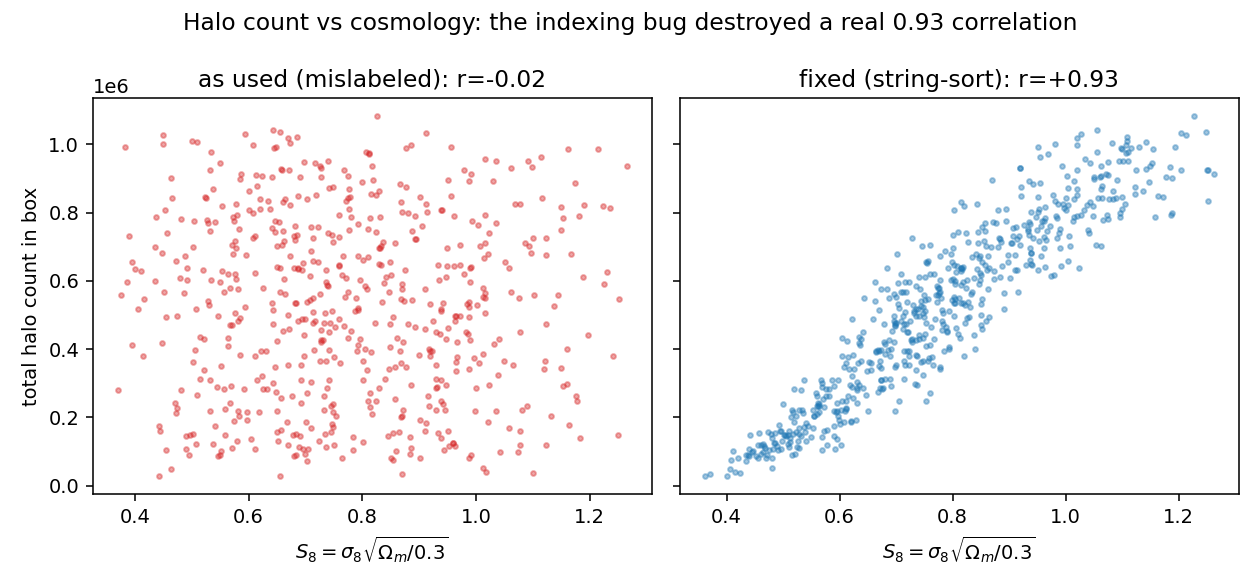
\includegraphics[width=0.85\linewidth]{figures_cmass/labelbug_count_vs_s8.png}
\caption{The indexing bug in one picture. Total halo count in a box against
$S_8 = \sigma_8\sqrt{\Omega_m/0.3}$. As the pipeline used the labels (left) the
correlation is zero; with the string-sort mapping corrected (right) the true
$0.93$ correlation reappears. Halo abundance must track $S_8$, so the left panel
was the signature of a labeling error, not of uninformative data.}
\label{fig:srs-labelbug}
\end{figure}

\paragraph{What this changes, and what it does not.} Every cosmology number we
computed before this point used the labels and is affected; the earlier
cross-fidelity tables have been removed and are replaced by the corrected results
below, and the earlier reading that the SR-versus-LR difference was an irreducible
coin flip was itself a product of the mislabeling. The results that do not use the
labels are unaffected and still stand: the power spectrum match of SR to HR, the
held-out bispectrum, the field-match statistics, the seam test, and the real space
error. The generator conditions on the cosmology as a style vector and was trained
with the scrambled labels, so its conditioning was uninformative during training;
we return to this at the end.

\paragraph{The data is informative after all.} With correct labels the picture
inverts. A halo count in this suite carries a strong cosmological signal: the
total halo count alone correlates with the combination $S_8 = \sigma_8
\sqrt{\Omega_m/0.3}$ at $0.93$ and with $\Omega_m$ at $0.85$. A Fisher forecast on
a single-box power spectrum now explains $98\%$ of the variance, where it
explained $0.2\%$ before, and it constrains $\Omega_m$ and $\sigma_8$ well, with
$\Omega_b$, $h$ and $n_s$ weak or unconstrained, which is the textbook pattern for
a low-redshift halo field. The field-level network tells the same story: after the
fix its predicted $\Omega_m$ correlates with the truth at $0.90$ on both training
and test boxes, where before the fix the correlation was zero and the output was a
constant. So the earlier conclusion that a single box carries almost no cosmology
was an artifact of the labeling, not a property of the data.

\begin{figure}[h]
\centering
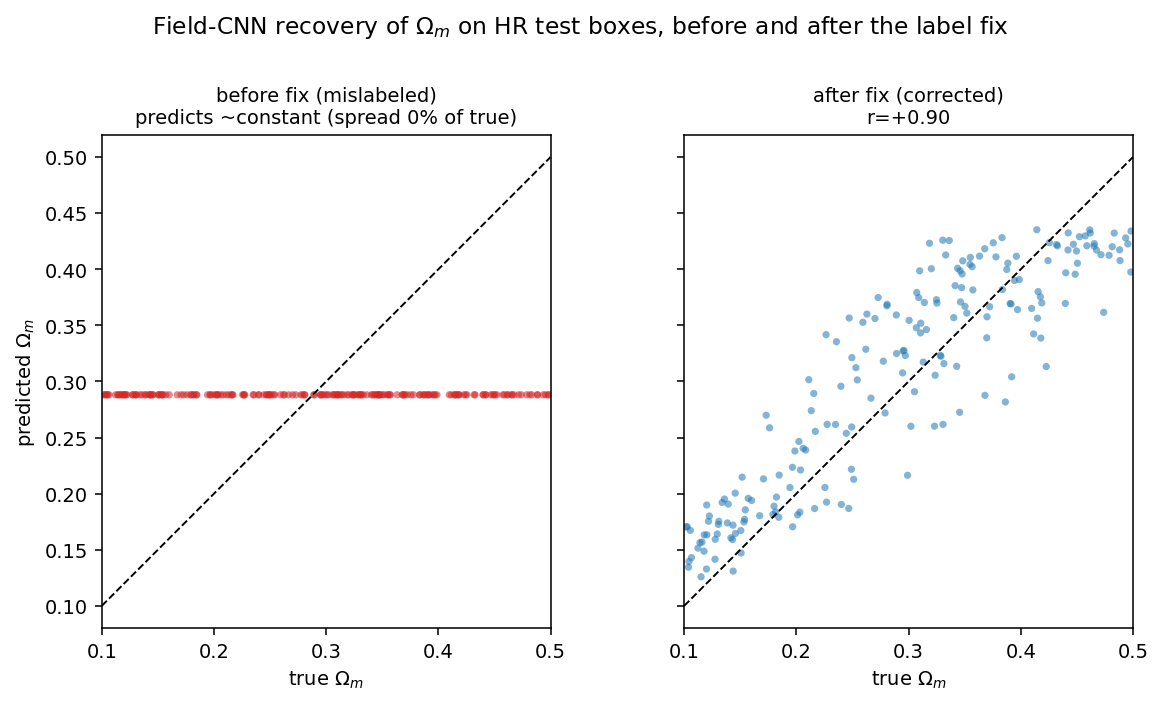
\includegraphics[width=0.82\linewidth]{figures_cmass/field_recovery_Om_cmass.png}
\caption{Field-level CNN recovery of $\Omega_m$ on HR test boxes, before and after
the label fix. Before (left) the prediction is flat and uncorrelated with the
truth (the network returns a near-constant); after (right) it tracks the diagonal
at a correlation of about $0.90$, on both training and test boxes. Same
architecture, same data, only the labels changed.}
\label{fig:srs-recovery}
\end{figure}

\begin{figure}[h]
\centering
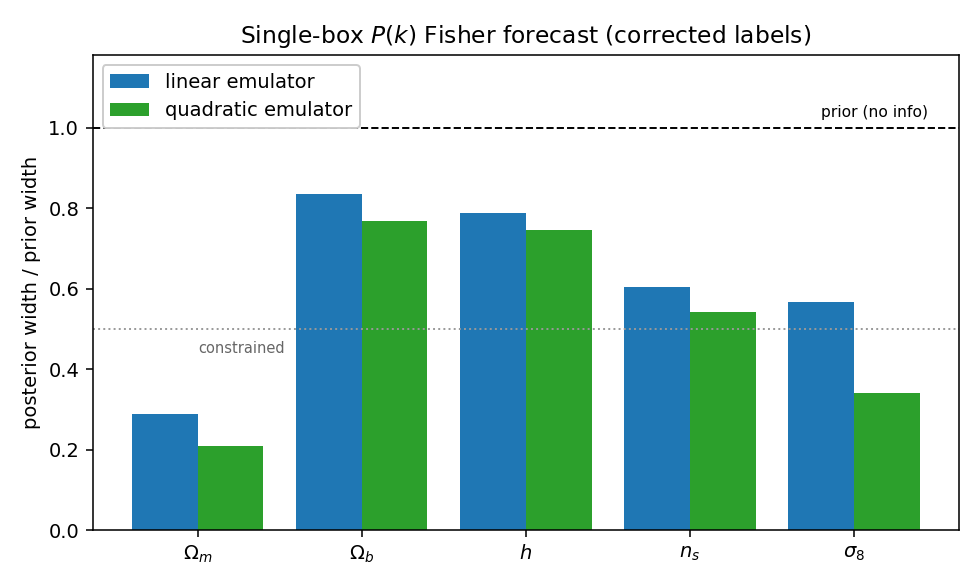
\includegraphics[width=0.72\linewidth]{figures_cmass/fisher_corrected_cmass.png}
\caption{Fisher forecast for a single-box power spectrum with corrected labels:
posterior width divided by prior width per parameter (lower means better
constrained, $1$ means no information). $\Omega_m$ is well constrained and
$\sigma_8$ is constrained, while $\Omega_b$, $h$ and $n_s$ are weak, the textbook
pattern for a low-redshift halo field. Two emulators (linear average slope and
quadratic at the prior centre) bracket the estimate.}
\label{fig:srs-fisher}
\end{figure}

\paragraph{Corrected cross-fidelity, and where SR helps.} We re-ran the goal
metric with correct labels at two levels, the power spectrum summary and the full
field. We train the posterior on one source, apply it to HR, and compare to a
posterior trained on HR, using an ensemble of independently retrained estimators
so the numbers are not single draws. Table~\ref{tab:srs-corrected} gives the
result.
\begin{table}[h]
\centering
\caption{Corrected cross-fidelity KL to HR (posterior trained on the named source,
evaluated on HR), lower is better, with the HR-to-HR floor for reference. Summary
uses the power spectrum; field uses a three-dimensional CNN posterior on the full
box.}
\label{tab:srs-corrected}
\begin{tabular}{lccc}
\toprule
level & LR (raw) & SR & HR floor \\
\midrule
summary $P(k)$ & $0.032$ & $0.088$ & $0.028$ \\
field (CNN)    & $0.49 \pm 0.81$ & $\mathbf{0.024}$ & $0.022$ \\
\bottomrule
\end{tabular}
\end{table}
\begin{figure}[h]
\centering
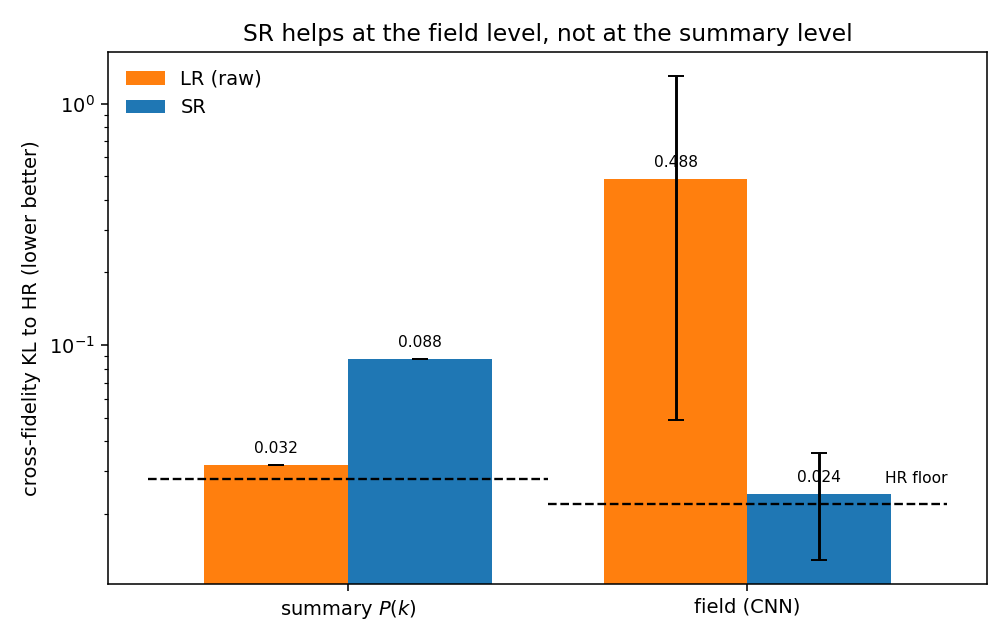
\includegraphics[width=0.7\linewidth]{figures_cmass/crossfid_corrected_cmass.png}
\caption{Corrected cross-fidelity KL to HR (log scale, lower is better) at the two
levels, with the HR-to-HR floor shown as the dashed line. At the summary level the
raw LR field is already at the floor and SR does not help. At the field level, an
LR-trained posterior does not transfer to HR (large and unstable), while an
SR-trained posterior sits at the floor. SR helps exactly where it corrects the
field.}
\label{fig:srs-crossfid-corrected}
\end{figure}
The two levels point in opposite directions, and both make sense. At the summary
level the raw LR power spectrum is already at the HR floor, so an LR-trained
posterior transfers to HR as well as an HR-trained one does, and there is no gap
for SR to close; SR even hurts a little, because the generator reshapes the
small-scale power in a way that does not match how HR responds to cosmology. At
the field level the raw LR box looks different enough from HR that an LR-trained
posterior does not transfer, and it does so unreliably, sometimes acceptably and
sometimes catastrophically, which is why its number carries such a large spread.
SR corrects the field to look like HR, so an SR-trained posterior transfers to HR
reliably, at the floor. This is exactly the deployment case the project is built
on, train the inference model on cheap SR-corrected boxes and apply it to
expensive HR, and at the field level SR makes it work where raw LR does not.

\paragraph{Padding on the goal metric.} We ran the two padding variants through
the corrected cross-fidelity at the summary level as well
(Table~\ref{tab:srs-padding}). Among the SR models the ordering from the earlier
report survives: no padding is best on the goal metric, trim-aware padding is
worse, and trim-unaware is worst, so for the cosmology objective the no-padding
model is the one to use. All three sit above the raw LR control at this level,
consistent with LR already being HR-like on the power spectrum. One number does
change under the fix: the mislabeled data made trim-unaware look catastrophic (a
factor of several hundred above the others), while with correct labels it is the
weakest variant by about a factor of two, not a blow-up. Its real-space error
(Figure~\ref{fig:srs-protocolv2}) remains the clearest and most direct sign that
it is the least reliable model.
\begin{table}[h]
\centering
\caption{Corrected cross-fidelity KL to HR at the summary (power spectrum) level
for the SR padding variants, with the LR control and the HR floor. Lower is
better. Field-level padding numbers are future work.}
\label{tab:srs-padding}
\begin{tabular}{lc}
\toprule
model & summary cross-fidelity KL \\
\midrule
SR, no padding & $\mathbf{0.087}$ \\
SR, trim-aware padding & $0.127$ \\
SR, trim-unaware padding & $0.172$ \\
\midrule
LR (control) & $0.031$ \\
HR floor & $0.028$ \\
\bottomrule
\end{tabular}
\end{table}

\paragraph{Bottom line.} With the labels fixed, the cosmology question has a
clear answer. The data constrains $\Omega_m$ and $\sigma_8$ from a single box. At
the power spectrum level the raw LR field is already HR-like, so SR is not needed
there and slightly hurts. At the field level, which is what SR actually corrects,
an SR-trained posterior transfers to HR at the floor while a raw LR one does not,
so SR provides a real and reliable cosmology benefit exactly where it operates.
Trim-unaware padding is still the weakest variant, worst on the goal metric and
on real-space error, though the label fix shrinks its apparent failure from
catastrophic to about a factor of two. Two honest caveats remain: the
field-level LR number has a wide spread and rests on a handful of retrained
networks, so the size of the gap should be firmed up with more seeds; and because
the generator was trained with the scrambled labels, its cosmology conditioning
was uninformative, so a retrain with correct conditioning may sharpen the SR
result further. Neither caveat changes the direction: with correct labels, SR
helps cosmology at the field level.

\paragraph{A data reliability note.} Partway through these runs, the shared
data storage this project reads from filled up completely, which caused a few
training jobs to fail with a file briefly appearing missing even though it was
not actually deleted. We added a retry step to the data loader and resumed
each affected run from its last saved checkpoint, so no real training progress
was lost. This is a shared infrastructure issue, not a problem with the data or
the method.

\subsection{Files}
\begin{itemize}\itemsep0pt
  \item Data and patching: \texttt{data/patch\_dataset\_cmass.py}
  (shared ops in \texttt{data/patch\_dataset\_real.py})
  \item Model: \texttt{map2map/models/styled\_srsgan.py}
  (\texttt{G\_correct}, \texttt{D\_const})
  \item Training: \texttt{train\_patch\_cmass.py};
  run script \texttt{scripts/train\_patch\_cmass.slurm}
  \item Inference and stitching: \texttt{infer\_stitch\_cmass.py}
  \item Seam eval: \texttt{analysis/eval\_seam\_cmass.py}
  \item Box / per-patch diagnostics: \texttt{analysis/diag\_cmass.py}
  \item SR-vs-HR match stats: \texttt{analysis/match\_stats\_cmass.py}
  \item SR-vs-HR power-spectrum figure: \texttt{analysis/plot\_sr\_vs\_hr.py}
  \item Bispectrum (held-out statistic): \texttt{analysis/bispectrum\_cmass.py}
  \item Training loss curves: \texttt{analysis/plot\_losses\_cmass.py}
  \item Cross-fidelity posterior evaluation: \texttt{evaluate.py} (SR-trained
  or LR-trained posterior evaluated on HR $P(k)$)
  \item Protocol-v2 (no-Pk-loss, padding-variant) training curves:
  \texttt{analysis/plot\_protocolv2\_cmass.py}
  \item Power spectrum on counts: \texttt{analysis/power\_spectrum.py}
  (estimator \texttt{counts}); differentiable training version
  \texttt{analysis/pk\_torch.py}
  \item Posterior and KL: \texttt{inference/nde.py}, \texttt{evaluate.py};
  end-to-end eval \texttt{scripts/eval\_cmass\_wrapper.slurm}
  \item Field-level posterior (three-dimensional CNN, moment-network loss):
  \texttt{models/field\_cnn.py}, \texttt{train\_field\_cnn.py};
  SR field generation \texttt{gen\_sr\_fields.py}; capacity and recovery
  diagnostics \texttt{overfit\_test.py}, \texttt{field\_diag.py}
  \item Outputs: \texttt{runs/patch\_cmass/}; figures: \texttt{figures\_cmass/}
\end{itemize}
 from main.tex, or paste inline.
% Figures referenced live in figures_cmass/ (set \graphicspath or copy them
% next to main.tex). Every number is from runs/patch_cmass/ and FINAL.md.
% =====================================================================

\section{SRS-styled-map2map-galaxy}
\label{sec:srs}

This section documents the second model in this work at the same level of
detail as \S5. Where \S5 corrects a Lagrangian \emph{displacement} field with a
point--voxel flow matcher, this model corrects an Eulerian \emph{halo count}
field with a styled GAN. The two share the same high-level goal, make a cheap
low-fidelity (LF) simulation look like an expensive high-fidelity (HF) one, 
but operate on different data and use a different architecture.

\paragraph{Goal.} Running an accurate (high-resolution) N-body simulation is
expensive; running a fast approximate one is cheap. We want a model that takes
\emph{only} the cheap LF field and produces a corrected field (we call it the
super-resolved or \textbf{SR} field) that matches the expensive HF field. At
inference the model never sees HF: the HF field is used only to train the model
and to grade it. So every result in this section answers one question: \emph{how
close is the SR field, built from LF alone, to the HF field it never saw?}

\paragraph{Terminology.} We work one cubic sub-volume at a time. We call the
$64^3$ output sub-volume a \textbf{core}, and the (possibly larger) input
sub-volume that the model reads a \textbf{patch}. When \texttt{pad}${=}0$ the
patch and the core coincide. We use \textbf{LR}/\textbf{LF} and
\textbf{HR}/\textbf{HF} interchangeably; the data here is named LR (input) and
HR (target).

\paragraph{Two arms.} We test the boundary treatment with two arms that are
identical except for one number:
\begin{itemize}
  \item \textbf{Arm A (naive, mentor 2.1):} \texttt{pad}${=}0$. Each $64^3$ core
  is corrected and placed edge-to-edge.
  \item \textbf{Arm B (overlap, mentor 2.2):} \texttt{pad}${=}8$. Each patch is
  grown to $80^3$ with real neighbour cells (periodic wrap), only the central
  $64^3$ core is kept and placed.
\end{itemize}

\subsection{Data Preprocessing}
\textit{Source: \texttt{cmass-ili}; loader \texttt{data/patch\_dataset\_cmass.py}.}

\paragraph{Input.} We have $2000$ paired simulations at redshift $z=0.5$, run
from shared initial conditions. Each pair is a low-fidelity field (LR, from the
FastPM particle-mesh code) and a high-fidelity field (HR, from a Quijote N-body
run). Both are stored as integer \textbf{halo count grids} of shape
$128\times128\times128$ on a periodic box of side $L_\text{box}=1000\
\mathrm{Mpc}/h$ (cell size $\approx 7.81\ \mathrm{Mpc}/h$). A cell value is the
number of halos whose position falls in that cell. The fields are sparse: most
cells are zero and the mean count per cell is small (the code caches one global
count scale, the mean HR count per cell measured over $50$ training sims).
Because LR and HR share initial conditions, they describe the same structure at
two fidelities. The correspondence is between the two halo catalogs \emph{as a
whole}: there is no known one-to-one matching between individual LR and HR
halos, only between the count fields they produce.

\paragraph{Cosmology labels.} Each simulation carries a style vector
$\mathbf s=(\Omega_m,\Omega_b,h,n_s,\sigma_8)\in\mathbb R^5$, parsed from that
sim's \texttt{config.yaml}.

\paragraph{Splits.} The on-disk lists give $1600$ train, $200$ validation, and
$200$ test simulations, split by simulation index.

\begin{figure}[t]
\centering
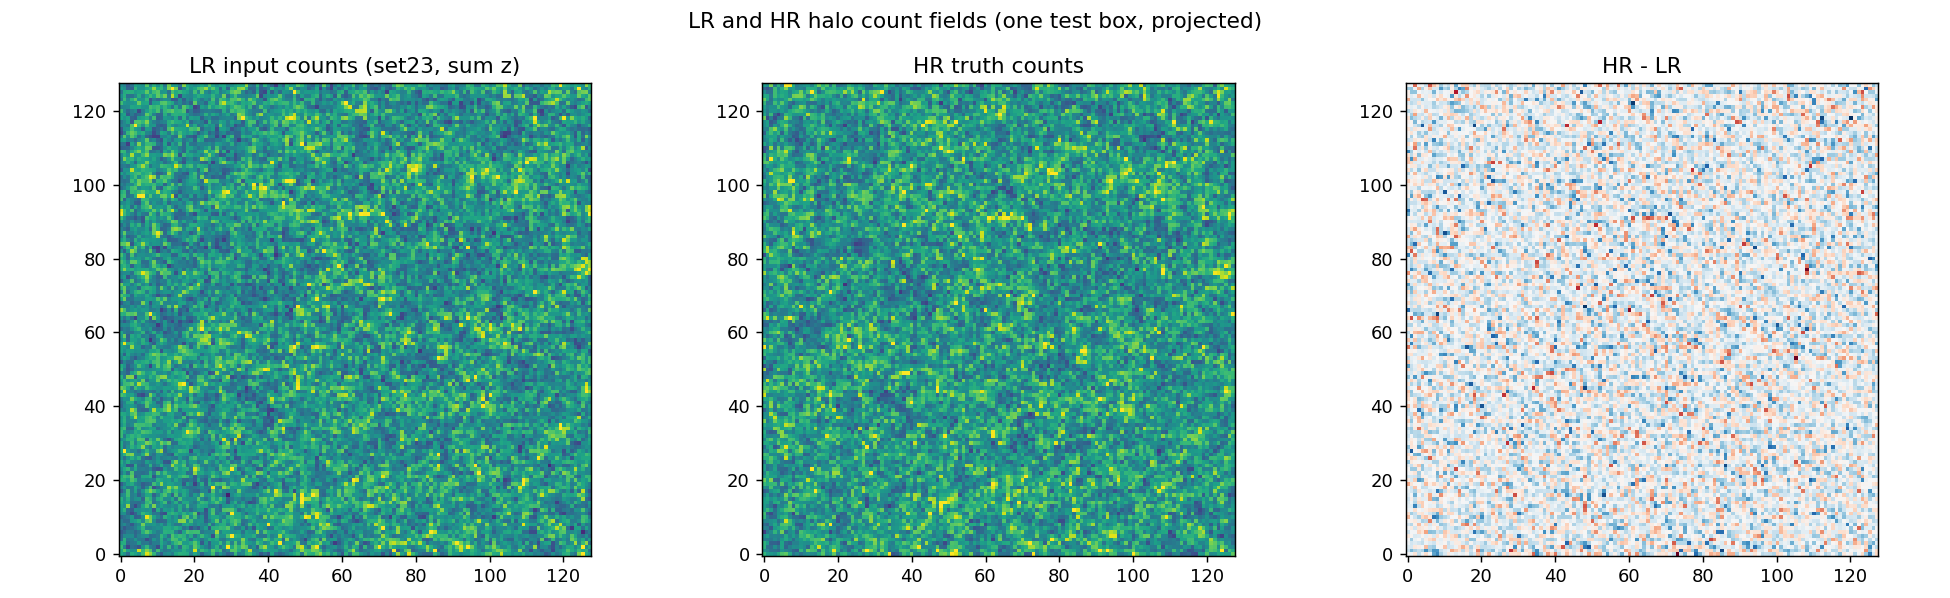
\includegraphics[width=0.9\linewidth]{figures_cmass/data_pair.png}
\caption{One LR/HR pair (projected count map). LR (FastPM, input) and HR
(Quijote N-body, target) share initial conditions and so share large-scale
structure, but differ cell-by-cell.}
\label{fig:srs-datapair}
\end{figure}

\paragraph{Model space (count transform).} The network does not learn on raw
counts; it learns in a compressed ``model space''. The default transform is
$\log(1+n)$, which tames the sparse heavy tail:
\begin{equation}
  y = \log(1+n), \qquad n = \exp(y)-1 \ \ (\text{clamped to } n\ge 0).
  \label{eq:srs-transform}
\end{equation}
Two alternative transforms exist in the code (\texttt{scale}: $n/\text{scale}$;
\texttt{delta}: model space is the overdensity itself), but all reported runs use
$\log(1+n)$. Power spectra are \emph{never} computed in model space; they are
always computed on the physical-count overdensity \SG{Is it okay if this is -1 when there are 0 halos?}
\begin{equation}
  \delta = \frac{n}{\bar n} - 1,
  \label{eq:srs-delta}
\end{equation}
with $\bar n$ the per-box mean count (the \texttt{perbox} setting used in all
runs).

\subsection{Data Pipeline (patching)}
\textit{Located in: \texttt{data/patch\_dataset\_cmass.py},
\texttt{data/patch\_dataset\_real.py} (shared patch ops).}

A model never sees the whole $128^3$ box at once. We cut the box into a
$2\times2\times2$ grid of $64^3$ \textbf{cores} (Table~\ref{tab:srs-notation}).
The cores tile the box exactly (stride $64$), so they reconstruct the box
bit-for-bit with no gaps and no double counting, the dataset's self-test
asserts this. Each model \emph{input} is a core grown by \texttt{pad} voxels on
every side, taken from the true neighbour cells with periodic wrap at the box
edge (\texttt{extract\_patch} uses \texttt{numpy.take(\dots, mode="wrap")}). So
with \texttt{pad}${=}8$ the input is $80^3$ and neighbouring patches overlap by
$2\cdot\texttt{pad}=16$ voxels; the HR \emph{target} is always the bare $64^3$
core. Because each simulation is one continuous periodic box that we crop
ourselves, the patches are real neighbours by construction, there is no data
seam (unlike the Lagrangian patches of \S5). \SG{Isn't the patch construction same in both?}

\begin{table}[t]
\centering
\caption{Notation for the CMASS count-field pipeline.}
\label{tab:srs-notation}
\begin{tabular}{llp{7.2cm}}
\toprule
Symbol & Value & Meaning \\
\midrule
$N_\text{full}$    & $128$ & full box side (voxels) \\
$P$ (\texttt{PATCH}) & $64$ & core side (voxels) \\
$N_\text{patches}$ & $8$ & cores per box ($2{\times}2{\times}2$) \\
\texttt{pad}       & $0$ (Arm A) / $8$ (Arm B) & halo width added to each face by periodic wrap \\
$L_\text{box}$     & $1000\ \mathrm{Mpc}/h$ & box side \\
$\mathbf s$        & $\in\mathbb R^5$ & cosmology vector $(\Omega_m,\Omega_b,h,n_s,\sigma_8)$ \\
$\bar n$           & per-box mean & mean count used to form $\delta=n/\bar n-1$ \\
\bottomrule
\end{tabular}
\end{table}

\begin{figure}[t]
\centering
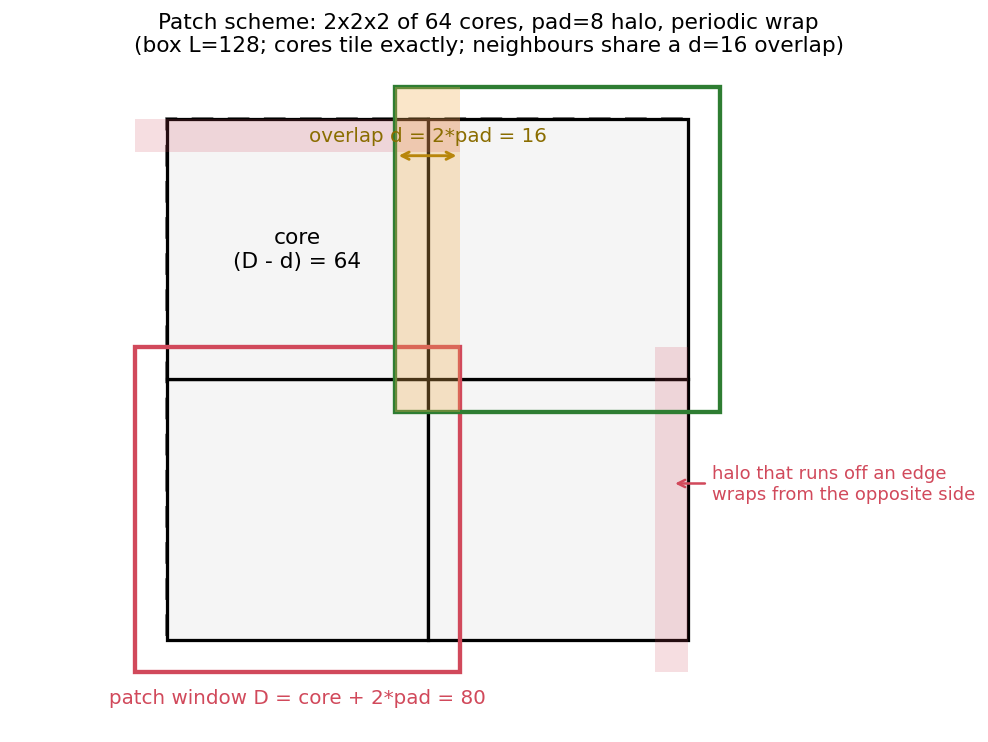
\includegraphics[width=0.82\linewidth]{figures_cmass/pipeline_patching.png}
\caption{Patch scheme. The box is cut into a $2{\times}2{\times}2$ grid of
$64^3$ cores that tile it exactly. With \texttt{pad}${>}0$ each patch is grown by
a halo of real neighbour cells (periodic wrap); only the central core is kept
and placed back.}
\label{fig:srs-patching}
\end{figure}

\paragraph{Per-simulation item.} Indexed by simulation, the dataset returns, for
all $8$ cores at once: the LR patches \texttt{lr\_in} of shape
$(8,\,1,\,64{+}2\,\texttt{pad},\,\cdot,\,\cdot)$ in model space, the HR cores
\texttt{hr\_tgt} of shape $(8,\,1,\,64,\,64,\,64)$, the style $\mathbf s$, and
the simulation index. The trainer flattens the $8$-core axis into the batch.

\begin{algorithm}[H]
\caption{\textsc{ExtractPatches} (one simulation)}
\label{alg:srs-extract}
\begin{algorithmic}[1]
\Require LR box $\mathbf L\in\mathbb R^{1\times128^3}$, HR box $\mathbf H$, \texttt{pad}
\State map $\mathbf L,\mathbf H$ to model space via Eq.~\ref{eq:srs-transform}
\For{$p=0,\dots,7$}
  \State $(i,j,k)\gets\textsc{unravel}(p,(2,2,2))$ \Comment{core origin $(64i,64j,64k)$}
  \State $\mathbf L_p\gets$ core $p$ grown by \texttt{pad} on each face, periodic wrap \Comment{$(64{+}2\,\texttt{pad})^3$}
  \State $\mathbf H_p\gets$ bare core $p$ \Comment{$64^3$}
\EndFor
\State \Return $\{(\mathbf L_p,\mathbf H_p)\}_{p=0}^{7}$, style $\mathbf s$
\end{algorithmic}
\end{algorithm}

\subsection{Model: Input/Output Specification}
\textit{Implementation: \texttt{map2map/models/styled\_srsgan.py}
(\texttt{G\_correct}, \texttt{D\_const}).}

\paragraph{What the generator computes.} The generator is a
\textbf{same-resolution residual} network: it does not change the grid size, and
it predicts a correction that is \emph{added} to the input. In model space,
\begin{equation}
  \mathrm{SR} \;=\; \mathrm{LR} \;+\; G(\mathrm{LR},\,\mathbf s,\,\mathbf z),
  \label{eq:srs-residual}
\end{equation}
where $\mathbf s$ is the cosmology vector and $\mathbf z$ is an injected noise
field (see below). Inputs and outputs are listed in
Table~\ref{tab:srs-model-io}; the generator is run once per core (the $8$ cores
of a box form a batch).

\begin{table}[t]
\centering
\caption{Tensors consumed/produced by the generator \texttt{G\_correct} for one
core (batch dimension omitted). Here $D=64{+}2\,\texttt{pad}$.}
\label{tab:srs-model-io}
\begin{tabular}{lll}
\toprule
Symbol & Shape & Meaning \\
\midrule
$\mathbf x$ (\texttt{x})       & $(1,D,D,D)$ & LR patch, model space (input) \\
$\mathbf s$ (\texttt{style})   & $(5,)$      & cosmology vector \\
$\mathbf z$ (\texttt{noise\_list}) & $2\cdot\texttt{num\_blocks}$ cubes $(1,D,D,D)$ & injected noise; fixed at inference, random in training \\
$G(\cdot)$                     & $(1,D,D,D)$ & predicted residual $\delta$ (added to $\mathbf x$) \\
\bottomrule
\end{tabular}
\end{table}

\paragraph{Internal composition.} $G$ is a constant-resolution StyleGAN2-style
network (no up/down-sampling), built from:
\begin{enumerate}
  \item \texttt{block0}: a $1{\times}1{\times}1$ style-modulated convolution
  (\texttt{ConvStyled3d}) lifting the $1$-channel input to $c_0$ channels,
  followed by a leaky ReLU.
  \item \texttt{num\_blocks} ($=4$) constant-resolution H-blocks
  (\texttt{HBlock\_const}). Each block, in order: inject noise $\to$
  $3{\times}3{\times}3$ \texttt{ConvStyled3d} (periodic ``circular'' padding)
  $\to$ leaky ReLU $\to$ inject noise $\to$ $3{\times}3{\times}3$
  \texttt{ConvStyled3d} $\to$ leaky ReLU $\to$ a $1{\times}1{\times}1$ projection
  to the output channel, accumulated into a running output $y$. The final return
  is $\mathbf x + y$ (Eq.~\ref{eq:srs-residual}).
\end{enumerate}
The channel widths come from \texttt{chan\_base} ($=128$) halved per block and
clamped to $[64,512]$. Two mechanisms make the convolutions depend on side
information:
\begin{itemize}
  \item \textbf{Style modulation.} \texttt{ConvStyled3d} is the StyleGAN2
  modulated/demodulated convolution: the cosmology vector $\mathbf s$ scales the
  convolution weights, so the same network behaves differently for different
  cosmologies. This is the only path by which $\mathbf s$ enters.
  \item \textbf{Noise injection.} Each \texttt{ConvStyled3d} is preceded by a
  per-channel learned-standard-deviation noise add (\texttt{\_NoiseInject}). At
  training time the noise is fresh Gaussian each call; at inference a
  \emph{fixed} list of noise cubes (seeded, built by \texttt{build\_noise\_list})
  is reused so outputs are reproducible. The noise is what lets the model produce
  a plausible small-scale field rather than a single blurred guess.
\end{itemize}

\paragraph{Discriminator.} \texttt{D\_const} is a constant-input-resolution
critic conditioned on the same style $\mathbf s$. It runs a head
\texttt{ConvStyled3d} then \texttt{num\_blocks} strided down-blocks (each a
periodic $3{\times}3{\times}3$ \texttt{ConvStyled3d} $+$ leaky ReLU $+$
$2{\times}$ average pool), a $1{\times}1{\times}1$ tail, and a final
$1{\times}1{\times}1$ projection to one channel, averaged over space to a single
logit per core.

\subsection{Training Step}
\textit{Located in: \texttt{train\_patch\_cmass.py}.}

The generator is trained per core (stitching is \emph{not} part of the
gradient). The total generator loss is a weighted sum of three terms,
\begin{equation}
  \mathcal L_G \;=\; \lambda_\text{adv}\,\mathcal L_\text{adv}
                  + \lambda_\text{rec}\,\mathcal L_\text{rec}
                  + \lambda_\text{pk}\,\mathcal L_\text{pk},
  \label{eq:srs-lossG}
\end{equation}
with (defaults from the original run script; see the protocol update below for
the values now in use):
\begin{itemize}
  \item \textbf{Reconstruction} $\mathcal L_\text{rec}=\lVert \mathrm{SR}-\mathrm{HR}\rVert_1$,
  a plain $L_1$ in model space (optionally Gaussian-smoothed; smoothing off in
  all runs).
  \item \textbf{Power-spectrum} $\mathcal L_\text{pk}$, the mean-squared error
  between the $\log_{10}$ power spectra of SR and HR, computed on the
  \emph{physical-count overdensity} of the $64^3$ core (Eqs.~\ref{eq:srs-transform}--\ref{eq:srs-delta}),
  Hann-windowed, with the HR side detached:
  \begin{equation}
    \mathcal L_\text{pk} = \frac{1}{|K|}\sum_{k\in K}
      \big(\log_{10} P_\text{SR}(k) - \log_{10} P_\text{HR}(k)\big)^2 .
    \label{eq:srs-pkloss}
  \end{equation}
  \item \textbf{Adversarial} $\mathcal L_\text{adv}=\mathrm{softplus}\!\big({-}D(\mathrm{SR},\mathbf s)\big)$,
  the non-saturating GAN generator loss.
\end{itemize}

\paragraph{Protocol update: what region the reconstruction and adversarial
terms see.} A \texttt{--pad-loss} setting controls how much of the generator's
output the $L_1$ and adversarial terms are computed on, independent of
\texttt{pad} itself:
\begin{itemize}
  \item \texttt{crop} (trim-aware, the setting used for Arm B above): the loss
  is computed only on \textsc{cropInterior}$(G(\mathbf x,\mathbf s),\,\texttt{pad})$,
  the $64^3$ core that is actually kept at inference time, against the bare
  $64^3$ HR core. The model is trained on exactly the region it will be graded
  on.
  \item \texttt{full}: the loss is computed on the whole $(64{+}2\,\texttt{pad})^3$
  output, against a correspondingly padded HR target (the dataset's
  \texttt{pad\_target} option). The model is trained as if the halo region it
  will later be trimmed off also mattered.
\end{itemize}
Concretely, let $\texttt{loss\_crop}=\texttt{pad}$ under \texttt{crop} and $0$
under \texttt{full}; every place above that writes $\mathrm{SR}$ means
$\textsc{cropInterior}(G(\mathbf x,\mathbf s),\,\texttt{loss\_crop})$, and the
Hann window and $P(k)$ estimator in $\mathcal L_\text{pk}$ are sized to match.
This is a controlled test of two ways padding could fail to help: see the
protocol-update subsection below for the result.

The discriminator is trained with the non-saturating GAN loss plus a lazy $R_1$
gradient penalty applied every \texttt{r1\_every} steps:
\begin{equation}
  \mathcal L_D = \mathrm{softplus}\!\big({-}D(\mathrm{HR})\big)
               + \mathrm{softplus}\!\big(D(\mathrm{SR})\big)
               + \tfrac{1}{2}\lambda_{R_1}\,\mathbb E\big\lVert \nabla_{\!x} D(x,\mathbf s)\big\rVert^2 .
  \label{eq:srs-lossD}
\end{equation}

\begin{algorithm}[H]
\caption{CMASS patch-GAN training step (one batch of cores)}
\label{alg:srs-train}
\begin{algorithmic}[1]
\Require LR patches $\mathbf x$, HR targets $\mathbf h$ (padded iff \texttt{pad-loss=full}),
         style $\mathbf s$, \texttt{pad}, \texttt{loss\_crop} ($=\texttt{pad}$ if \texttt{crop} else $0$),
         weights $\lambda_\text{adv},\lambda_\text{rec},\lambda_\text{pk},\lambda_{R_1}$
\Statex \textbf{// Discriminator}
\State $\hat{\mathbf h}\gets \textsc{cropInterior}\big(G(\mathbf x,\mathbf s),\,\texttt{loss\_crop}\big)$ \Comment{no grad}
\State $\mathcal L_D \gets \mathrm{softplus}({-}D(\mathbf h,\mathbf s)) + \mathrm{softplus}(D(\hat{\mathbf h},\mathbf s))$
\If{step $\bmod\ \texttt{r1\_every} = 0$} $\mathcal L_D \mathrel{+}= \tfrac12\lambda_{R_1}\texttt{r1\_every}\cdot R_1(D,\mathbf h,\mathbf s)$ \EndIf
\State update $D$ (Adam, grad-clip)
\Statex \textbf{// Generator}
\State $\hat{\mathbf h}\gets \textsc{cropInterior}\big(G(\mathbf x,\mathbf s),\,\texttt{loss\_crop}\big)$
\State $\mathcal L_\text{adv}\gets \mathrm{softplus}({-}D(\hat{\mathbf h},\mathbf s))$
\State $\mathcal L_\text{rec}\gets \lVert \hat{\mathbf h}-\mathbf h\rVert_1$
\State $\mathcal L_\text{pk}\gets$ Eq.~\ref{eq:srs-pkloss} on Hann-windowed overdensity of $\hat{\mathbf h}$, $\mathbf h$
       (skip if $\lambda_\text{pk}{=}0$)
\State $\mathcal L_G \gets \lambda_\text{adv}\mathcal L_\text{adv}+\lambda_\text{rec}\mathcal L_\text{rec}+\lambda_\text{pk}\mathcal L_\text{pk}$
\State update $G$ (Adam, grad-clip)
\end{algorithmic}
\end{algorithm}

\paragraph{Validation and checkpoint selection.} After each epoch we stitch the
full $128^3$ SR box for up to $40$ validation sims and report the stitched
$L_1$/voxel and the stitched-$128$ power-spectrum RMS against HR
(\S\ref{sec:srs-eval}, Eq.~\ref{eq:srs-pkrms}). A \texttt{--select} setting
chooses which of the two the saved \texttt{best.pt} tracks: \texttt{pk} (the
original setting, lowest stitched validation Pk RMS) or \texttt{l1} (lowest
stitched validation $L_1$/voxel). Selection is always on the stitched full box,
not the per-core training loss. Runs that also train with $\lambda_\text{pk}{=}0$
use \texttt{--select l1}, since selecting on Pk RMS while not training on it
would reintroduce the same metric leak in a different place.

\subsection{Inference}
\textit{Located in: \texttt{infer\_stitch\_cmass.py}.}

For one simulation: load the LR $128^3$ count box, map it to model space, run $G$
on each of the $8$ cores (with the periodic-wrap halo in Arm B), crop the halo,
stitch the cores into a $128^3$ model-space box, invert the transform to physical
counts, and clamp. \SG{are all outputs later mapped to integers, or are we fine with non-integer number of halos?} The injected noise list is fixed (seeded) so the output is
reproducible.

\begin{algorithm}[H]
\caption{CMASS inference + stitch (one simulation)}
\label{alg:srs-infer}
\begin{algorithmic}[1]
\Require LR box $\mathbf L$, style $\mathbf s$, trained $G$, mode (naive/overlap), fixed noise $\mathbf z$
\State $\texttt{pad}\gets 0$ if naive else value from checkpoint ($8$)
\State map $\mathbf L$ to model space (Eq.~\ref{eq:srs-transform})
\For{$p=0,\dots,7$}
  \State $\mathbf x_p\gets$ patch $p$ (core grown by \texttt{pad}, periodic wrap)
  \State $\mathbf c_p\gets \textsc{cropInterior}\big(G(\mathbf x_p,\mathbf s,\mathbf z),\,\texttt{pad}\big)$ \Comment{$64^3$ core, model space}
\EndFor
\State $\mathbf S\gets \textsc{stitch}(\{\mathbf c_p\})$ \Comment{$128^3$, model space}
\State $\mathbf S\gets \exp(\mathbf S)-1$, clamp to $[0,\,C_\text{max}{=}200]$, replace NaN/Inf \Comment{physical counts}
\State \Return $\mathbf S$
\end{algorithmic}
\end{algorithm}

\subsection{Crop Stitching}

Stitching is \textbf{direct placement with no averaging}. Adjacent cores tile the
box exactly (stride $64$, no overlap between cores once the halo is dropped), so
each core's $64^3$ output is written straight into its slot. In Arm B the $80^3$
patch is corrected and only its central $64^3$ core is kept; the overlap halo is
context for the convolution, never written to the output.

\begin{algorithm}[H]
\caption{\textsc{Stitch} ($8$ cores $\to$ $128^3$)}
\label{alg:srs-stitch}
\begin{algorithmic}[1]
\Require cores $\{\mathbf c_p\}_{p=0}^{7}$, each $1\times64^3$
\State $\mathbf S\gets \mathbf 0\in\mathbb R^{1\times128^3}$
\For{$p=0,\dots,7$}
  \State $(i,j,k)\gets\textsc{unravel}(p,(2,2,2))$
  \State $\mathbf S[:,\,64i{:}64i{+}64,\,64j{:}\cdots,\,64k{:}\cdots]\gets \mathbf c_p$ \Comment{direct assignment}
\EndFor
\State \Return $\mathbf S$
\end{algorithmic}
\end{algorithm}

\subsection{Evaluation}
\label{sec:srs-eval}
\textit{Located in: \texttt{analysis/eval\_seam\_cmass.py},
\texttt{analysis/diag\_cmass.py}, \texttt{analysis/match\_stats\_cmass.py},
\texttt{analysis/power\_spectrum.py}, \texttt{inference/nde.py},
\texttt{evaluate.py}.}

We evaluate the SR field against HR at three levels: a seam check (does stitching
leave a join?), field statistics (does SR have the right structure?), and
cosmology (does SR give the same parameter posterior as HR?).

\paragraph{Power-spectrum summaries.} On the count overdensity (Eq.~\ref{eq:srs-delta})
we report the power spectrum $P(k)$, the transfer ratio, and the cross-coherence:
\begin{equation}
  T(k) = \frac{P_\text{SR}(k)}{P_\text{HR}(k)},
  \qquad
  r(k) = \frac{P_{\text{SR},\text{HR}}(k)}{\sqrt{P_\text{SR}(k)\,P_\text{HR}(k)}} .
  \label{eq:srs-Tr}
\end{equation}
$T(k)=1$ means SR has the right \emph{amount} of power at scale $k$ (amplitude);
$r(k)=1$ means SR has the structure in the right \emph{place} (phase). The
scalar power-spectrum error used for checkpoint selection and seam reporting is
the log-RMS over the resolved $k$-bins:
\begin{equation}
  \mathrm{PkRMS}_{\log_{10}} = \sqrt{\frac{1}{|K|}\sum_{k\in K}
    \big(\log_{10} P_\text{SR}(k) - \log_{10} P_\text{HR}(k)\big)^2 } .
  \label{eq:srs-pkrms}
\end{equation}

\paragraph{Seam diagnostic.} \texttt{eval\_seam\_cmass.py} bins the per-cell
count error $|{\mathrm{SR}-\mathrm{HR}}|$ by distance to the nearest core face
and forms a per-position error profile along each axis. The headline number is
the \textbf{$x{=}64$ internal-seam excess}: the error on the internal core
boundary plane divided by the interior error. A value near $1$ means stitching
leaves no seam. The box edge $x{=}0$ is a periodic-boundary control.

\paragraph{Field-match statistics.} \texttt{match\_stats\_cmass.py} reports, over
$16$ test boxes: the total-count ratio $\sum\mathrm{SR}/\sum\mathrm{HR}$, the
void fraction (cells $<0.5$), the real-space cell standard-deviation ratio
$\mathrm{std}(\mathrm{SR})/\mathrm{std}(\mathrm{HR})$ (a blur check), and the
cross-coherence $r(k)$ at large ($k<0.05$) and small ($k>0.2$) scales.

\paragraph{Cosmology (posterior consistency).} This is the strongest ``does SR
match HR'' test. We voxel-count $\to$ overdensity $\to$ $P(k)$ for every box, then
train a neural density estimator $q(\theta\mid P(k))$ on the training split using
\texttt{sbi} (\texttt{SNPE\_C} with a neural-spline-flow density estimator,
\texttt{inference/nde.py}); the summary is $\log_{10}P(k)$. We train one estimator
on HR ($q_\text{HR}$) and one on each SR arm ($q_\text{SR}$). For each test box we
draw $2000$ posterior samples from each, fit a Gaussian per parameter, and report
the per-parameter Gaussian KL (\texttt{evaluate.py}):
\begin{equation}
  \mathrm{KL}\big(\mathcal N(\mu_\text{HR},\sigma_\text{HR})\,\Vert\,\mathcal N(\mu_\text{SR},\sigma_\text{SR})\big)
  = \tfrac12\!\left[\log\frac{\sigma_\text{SR}^2}{\sigma_\text{HR}^2}
    + \frac{\sigma_\text{HR}^2+(\mu_\text{HR}-\mu_\text{SR})^2}{\sigma_\text{SR}^2} - 1\right].
  \label{eq:srs-kl}
\end{equation}
$\mathrm{KL}=0$ means SR gives the identical cosmology posterior to HR. The raw LR
field (no model), pushed through the same pipeline, is the control SR must beat.

We report this comparison in two forms, and it matters which is which:
\begin{itemize}
  \item \textbf{Cross-fidelity (primary).} $q_\text{SR}$ is trained on SR power
  spectra but \emph{evaluated on the HR} $P(k)$ of each test simulation, and
  compared to $q_\text{HR}$ evaluated on the same HR $P(k)$. This is the
  deployment scenario the project targets: HR simulations are too expensive to
  train an inference model on, so the inference model is trained on cheap SR
  output and must still work when applied to (HR-like) reality. The comparison
  against an LR-trained estimator on the same HR data measures whether sampling
  in HR space (SR) survives the distribution shift better than staying in LR
  space. This metric never appears in the training loss.
  \item \textbf{Own-data (secondary).} $q_\text{SR}$ trained and evaluated on SR
  vs $q_\text{HR}$ trained and evaluated on HR, each pipeline end-to-end on
  its own field type.
\end{itemize}

\subsection{Best-Run Configuration}
\textit{Run script: \texttt{scripts/train\_patch\_cmass.slurm}; checkpoints
\texttt{checkpoints/patch\_cmass\_\{A,B\}/best.pt}.}

Both arms use the identical configuration below; they differ only in \texttt{pad}
($0$ for Arm~A, $8$ for Arm~B). This is the configuration behind every number
in \S\ref{sec:srs-results}--\S\ref{sec:srs-next}.

\begin{lstlisting}[language=bash]
--transform log1p   --nbar perbox        # log(1+n) model space; per-box nbar
--epochs 30         --sims-per-batch 1    # patch-batch = 8 cores per step
--chan-base-g 128   --chan-base-d 64  --num-blocks 4
--lambda-adv 1.0    --lambda-rec 2.0  --lambda-pk 2.0   # generator weights
--lambda-r1 10.0    --r1-every 16                       # lazy R1
--lr-g 1e-4 --lr-d 1e-4  --beta1 0.0 --beta2 0.99       # Adam
--grad-clip 1.0     --val-max-sims 40    --select pk    # select on Pk RMS
\end{lstlisting}

The best checkpoint per arm is the one with the lowest stitched validation Pk RMS
(Eq.~\ref{eq:srs-pkrms}):

\begin{center}
\begin{tabular}{lc}
\toprule
arm & best stitched val PkRMS$_{\log_{10}}$ \\
\midrule
Arm A, naive (pad $0$)  & $0.0947$ \\
Arm B, overlap (pad $8$) & $0.0963$ \\
\bottomrule
\end{tabular}
\end{center}

\paragraph{Protocol update.} Following the mentor meeting reported in
\S\ref{sec:srs-followup}, the configuration above is no longer the one we train
with. Three settings changed:
\begin{lstlisting}[language=bash]
--lambda-pk 0.0      # power-spectrum term OFF (it was also our main metric)
--pad-loss crop|full # trim-aware vs trim-unaware padding, see below
--select l1          # select on stitched L1, not the term we removed
\end{lstlisting}
All results in \S\ref{sec:srs-followup} use this configuration. Runs under the
original configuration above (Arm A, Arm B, and everything derived from them in
\S\ref{sec:srs-results}--\S\ref{sec:srs-next}) remain valid as a record of that
protocol; they are superseded, not invalidated, by the update.

\subsection{Results: Does SR Match HR?}
\label{sec:srs-results}

All numbers are on the $200$-box test split unless noted.

\paragraph{1. Power spectrum (statistics).} Across the test set the SR power
spectrum tracks HR at every scale, and Arm A beats the no-model LR control on the
overall log-RMS (Fig.~\ref{fig:srs-srvshr}, computed by
\texttt{analysis/plot\_sr\_vs\_hr.py}).

\begin{table}[h]
\centering
\caption{SR vs HR power-spectrum agreement, $200$ test boxes. Transfer
$T(k)=P_X/P_\text{HR}$ (Eq.~\ref{eq:srs-Tr}); $1.0$ is perfect.}
\label{tab:srs-pk}
\begin{tabular}{lccc}
\toprule
field (vs HR) & PkRMS$_{\log_{10}}$ & $T$ at large scales ($k{<}0.1$) & $T$ at small scales ($k{>}0.3$) \\
\midrule
SR (Arm A, naive)    & $\mathbf{0.0607}$ & $0.95$ & $1.04$ \\
SR (Arm B, overlap)  & $0.0645$ & $0.93$ & $0.88$ \\
LR (no model, control) & $0.0641$ & $1.01$ & $1.01$ \\
\bottomrule
\end{tabular}
\end{table}

\begin{figure}[t]
\centering
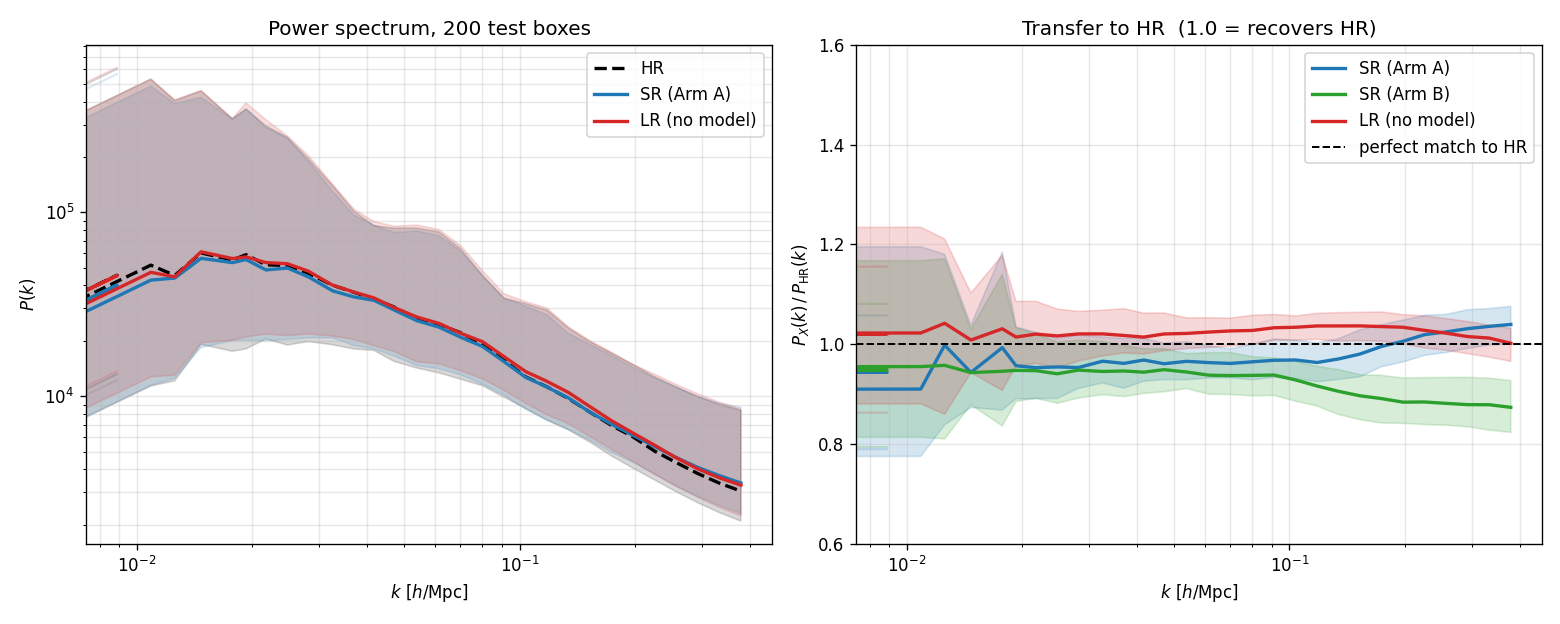
\includegraphics[width=0.98\linewidth]{figures_cmass/sr_vs_hr_pk.png}
\caption{\textbf{Left:} $P(k)$ of HR, SR (Arm A), and LR over $200$ test boxes
(median $+$ $16/84\%$ band). \textbf{Right:} transfer to HR; $1.0$ recovers HR.
SR (Arm A) sits near $1$ at all scales; Arm B's overlap blending slightly
suppresses small-scale power (transfer $0.88$).}
\label{fig:srs-srvshr}
\end{figure}

\paragraph{2. Field structure.} Beyond the power spectrum, SR keeps the field
structure of HR (Arm A, $16$ test boxes, \texttt{match\_stats\_cmassA.txt}):

\begin{table}[h]
\centering
\caption{SR vs HR field-match statistics (Arm A).}
\label{tab:srs-match}
\begin{tabular}{lll}
\toprule
quantity & value & reading \\
\midrule
total count ratio $\sum\mathrm{SR}/\sum\mathrm{HR}$ & $0.965\pm0.172$ & counts conserved on average; large per-box scatter \\
real-space std ratio & $1.008\pm0.100$ & clustering amplitude matches; not blurred \\
void fraction SR / HR ($<0.5$) & $0.855$ / $0.833$ & SR keeps voids empty, like HR \\
cross-coherence $r$, $k<0.05$ & $0.951$ & large-scale structure matches cell-by-cell \\
cross-coherence $r$, $k>0.2$ & $0.403$ & small-scale structure decorrelates \\
\bottomrule
\end{tabular}
\end{table}

\paragraph{3. Cosmology.} The cosmology comparison in the original report used
mislabeled cosmologies, an indexing bug we describe and fix in
\S\ref{sec:srs-correction}, so those numbers are not shown here. With correct
labels a single box constrains $\Omega_m$ and $\sigma_8$; at the power spectrum
level the raw LR field is already HR-like, while at the field level an SR-trained
posterior transfers to HR and an LR-trained one does not
(\S\ref{sec:srs-correction}, Table~\ref{tab:srs-corrected}).

\paragraph{4. Seam.} Neither arm introduces a stitching seam: the $x{=}64$
internal-seam excess is $\approx1$ for both
(Table~\ref{tab:srs-seam}, Fig.~\ref{fig:srs-seam}). Arm A shows a mild generic
ripple near \emph{any} boundary plane (seam-distance ratio $1.17$); Arm B's
overlap removes it ($1.00$) at a small cost in Pk RMS.

\begin{table}[h]
\centering
\caption{Seam and stitched-fidelity metrics, $200$ test boxes. ``Excess'' is
boundary error over interior error; $\approx1$ means no seam.}
\label{tab:srs-seam}
\begin{tabular}{lccp{5.2cm}}
\toprule
metric & Arm A naive & Arm B overlap & reading \\
\midrule
$x{=}64$ internal-seam excess & $0.9934$ & $0.9998$ & no internal seam either arm \\
seam-distance ratio ($d{=}0/d{\ge}8$) & $1.1729$ & $1.0032$ & generic boundary ripple, removed by overlap \\
$x{=}0$ periodic edge (control) & $0.9930$ & $0.9993$ & box edge behaves like interior \\
stitched PkRMS$_{\log_{10}}$ vs HR & $0.0637$ & $0.0678$ & stitched power-spectrum match \\
\bottomrule
\end{tabular}
\end{table}

\begin{figure}[t]
\centering
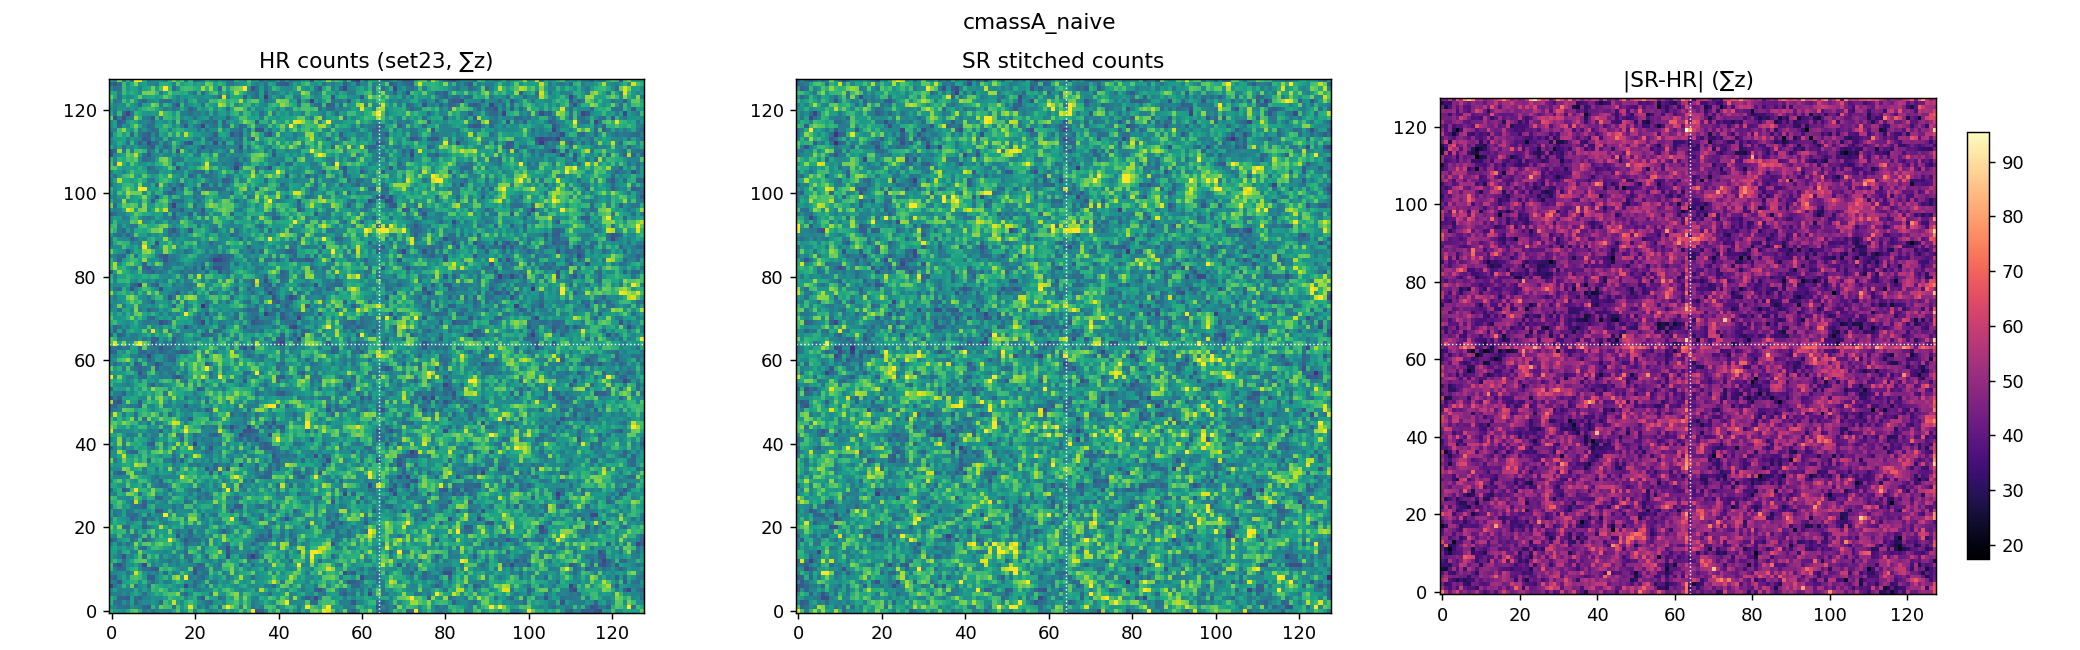
\includegraphics[width=0.95\linewidth]{figures_cmass/seam_cmassA_naive_slice.png}
\caption{Projected count maps for one test box (Arm A): HR, stitched SR, and the
absolute residual $|\mathrm{SR}-\mathrm{HR}|$. White dotted lines mark the
$x{=}64$, $y{=}64$ core boundaries; the residual shows no elevated ridge along
them.}
\label{fig:srs-seam}
\end{figure}

\paragraph{Per-scale diagnostic panels.} Figure~\ref{fig:srs-pkpanel} shows the
full-box $P(k)$, transfer, and cross-coherence for Arm A. The transfer sits near
$1$ at all scales (right amount of power); the cross-coherence is near $1$ at
large scales and falls toward small scales (structure placement is recovered at
large scales only). The per-patch panel
(\texttt{figures\_cmass/pk\_panel\_patch\_cmassAfix.png}) and the projection panels
(\texttt{projection\_box\_cmassAfix\_set23.png},
\texttt{projection\_patch\_cmassAfix\_set23\_p0.png}) tell the same story; Arm~B's
panels carry the \texttt{cmassB} suffix.

\begin{figure}[t]
\centering
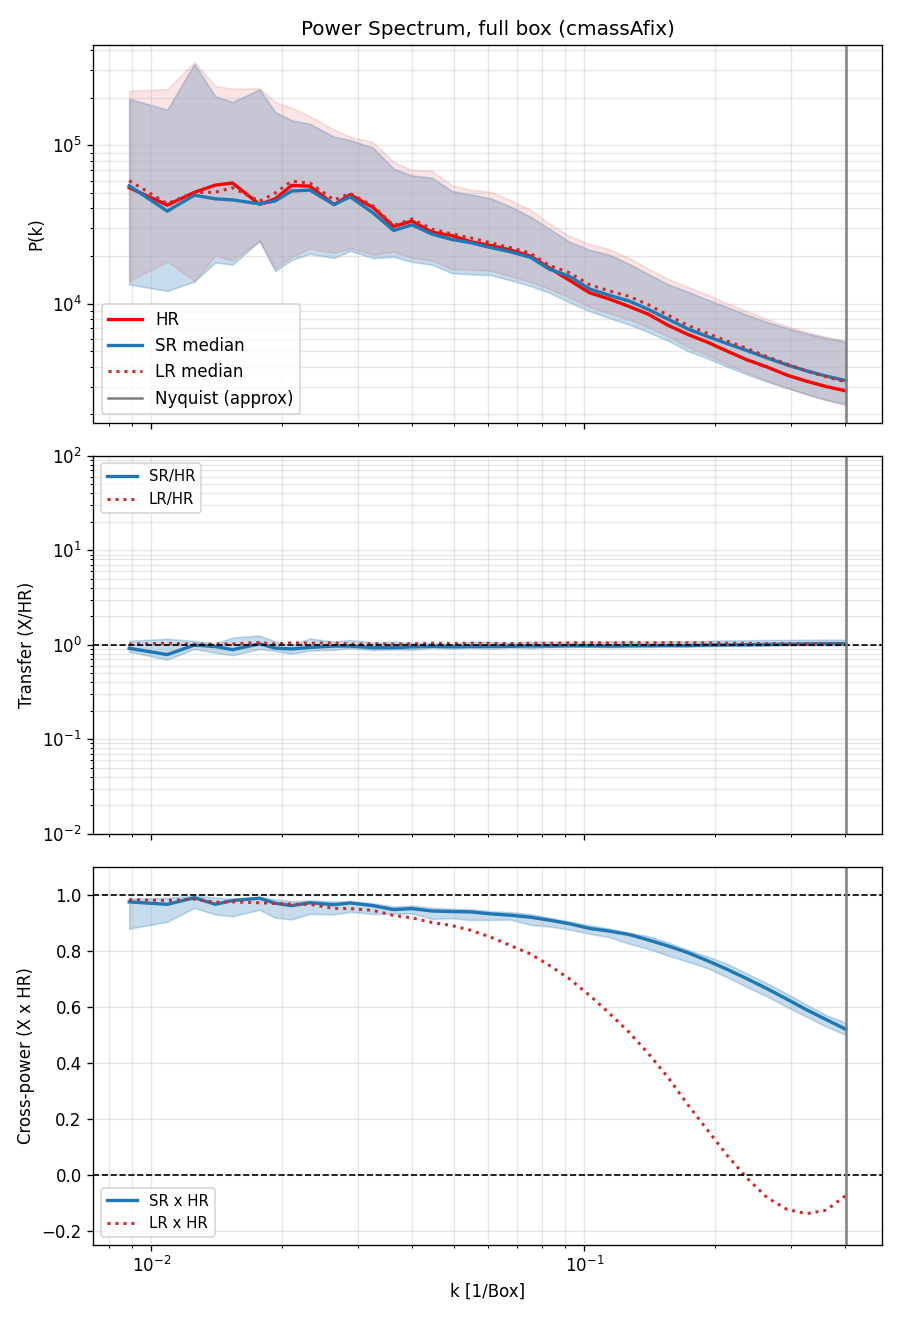
\includegraphics[width=0.5\linewidth]{figures_cmass/pk_panel_box_cmassAfix.png}
\caption{Full-box diagnostic for the conditioned generator (fiducial cosmology,
$16$ test boxes): $P(k)$ of HR (red), SR (blue median $+$ band), and LR (dotted
red); transfer $T(k)=P_X/P_\text{HR}$ on a linear axis with the 16 to 84
percentile band for both SR and LR, the legend reporting the RMS deviation of
each ratio from unity; and cross-coherence $r(k)$. The SR median transfer sits
below unity for $k<0.1$, a systematic large-scale power deficit of roughly 5 to
10 percent, while LR sits slightly above unity; SR does not tighten the transfer
scatter relative to LR. In $r(k)$, SR stays near unity to smaller scales while
LR decorrelates.}
\label{fig:srs-pkpanel}
\end{figure}

\subsection{Diagnostic: What is NOT Working}

\paragraph{Small-scale structure decorrelates, and this is fundamental.} SR
matches HR cell-by-cell at large scales ($r{=}0.95$ for $k<0.05$) but loses the
match at small scales ($r{=}0.40$ for $k>0.2$, Table~\ref{tab:srs-match}). This
is not a capacity bug: it is set by how much information the LR input carries
about HR. LR and HR share large-scale modes but the voxel-by-voxel LR$\leftrightarrow$HR
correlation is only $\approx0.06$, so the exact small-scale realization is simply
not present in the input. The model can match the small-scale \emph{statistics}
(transfer $\approx1$, real-space std ratio $1.008$) but cannot reproduce the
exact placement of individual halos. The noise injection
(Eq.~\ref{eq:srs-residual}) exists precisely because of this: it draws a
plausible small-scale field rather than regressing to a blur.

\paragraph{Per-box total-count scatter.} The total halo count is conserved on
average but with $\sim17\%$ per-box scatter ($\sum\mathrm{SR}/\sum\mathrm{HR}=
0.965\pm0.172$). A count-aware output head (predict a rate and sample Poisson
counts) would tighten this; it is the one clearly addressable imperfection. \SG{I would think this isn't necessary to fix, we don't care about the number of halos after all.}

\paragraph{Overlap suppresses small-scale power.} Arm B's overlap blending lowers
the small-scale transfer to $0.88$ (Table~\ref{tab:srs-pk}), so on the power
spectrum the naive Arm A is the better super-resolver. Overlap removes a small
generic boundary ripple but buys no fidelity, because on this continuous count
data there is no real seam to fix, the clean version of the mentor 2.1 vs 2.2
comparison.

\paragraph{Where the cosmology value is.} At the power spectrum level the raw LR
field is already close to HR, since they share large-scale modes, so the power
spectrum is a forgiving summary with little headroom. The model's value is at the
field level (variance, voids, small-scale structure), which the power spectrum
summary is insensitive to. The corrected cross-fidelity in
\S\ref{sec:srs-correction} bears this out: SR and LR are indistinguishable at the
power spectrum level, but at the field level an SR-trained posterior transfers to
HR while an LR-trained one does not.

\subsection{What I'm Trying Next}
\label{sec:srs-next}

The diagnostics above point to one limit that may be fundamental (small-scale
decorrelation) and a few that are clearly fixable (count scatter, small-scale
realism). The plan below is ordered so that we \emph{measure} the limit before
spending effort trying to beat it. None of these results are in yet; this is the
roadmap, not an experiment log.

\paragraph{Step 0, measure the information ceiling first.} Before trying to
improve the small-scale match, we need to know whether $r{=}0.40$ at small scales
(Table~\ref{tab:srs-match}) is the best any model could do from this input, or a
weakness of the current one. Two cheap diagnostics settle it:
\begin{itemize}
  \item \textbf{LR$\leftrightarrow$HR cross-coherence $r_\text{LR,HR}(k)$.} The
  cross-coherence of the \emph{raw input} against HR (no model) is the ceiling:
  no function of LR can place small-scale structure better than the input
  already correlates with HR. If $r_\text{SR,HR}(k)\approx r_\text{LR,HR}(k)$ at
  small $k$, the model is already at the ceiling and the limit is fundamental;
  if it sits well below, there is recoverable structure left on the table. (Only
  per-box $P(k)$ is currently saved, not the cross-spectrum, so this needs one
  re-run that keeps the fields.)
  \item \textbf{No-noise ablation.} Train the same generator with the noise
  injection off (a plain regressor). Theory predicts this should \emph{raise} the
  small-scale cross-coherence a little (a regressor targets the conditional mean,
  the best cell-by-cell predictor) but \emph{lower} the small-scale transfer well
  below $1$ (the conditional mean is blurry). Seeing exactly that trade-off would
  confirm that the noise/GAN is the right choice for a power-spectrum target, and
  would quantify how much cell-by-cell accuracy is being traded for correct
  statistics.
\end{itemize}

\paragraph{Step 1, fix the count scatter and small-scale realism (independent
of the ceiling).} These help regardless of what Step 0 finds:
\begin{itemize}
  \item \textbf{Count-aware (Poisson) output head.} Instead of predicting a
  count directly, predict a non-negative rate $\lambda$ per cell and sample the
  count as $n\sim\mathrm{Poisson}(\lambda)$. Halo counts are discrete and sparse,
  so a Poisson head models the small-scale graininess as actual shot noise rather
  than a smeared residual, and should tighten the $\sim17\%$ per-box total-count
  scatter (Table~\ref{tab:srs-match}), the one clearly addressable imperfection.
  \item \textbf{Explicit statistics terms in the loss.} Add a one-point PDF /
  variance matching term so small-scale sharpness is enforced directly, rather
  than relying on the adversarial term alone to find it.
  \item \textbf{Loss rebalance.} The current weights are $\lambda_\text{rec}{=}2$,
  $\lambda_\text{pk}{=}2$, $\lambda_\text{adv}{=}1$
  (Eq.~\ref{eq:srs-lossG}). The $L_1$ term blurs; lowering it and raising the
  adversarial weight should push toward correct statistics, at a known cost in
  cell-by-cell accuracy, per the same trade-off as the no-noise ablation.
\end{itemize}

\paragraph{Step 2, extract more of the available information (only if Step 0
shows headroom).} If $r_\text{SR,HR}$ sits below the LR$\leftrightarrow$HR
ceiling, the model is under-using its input. A larger receptive field, or feeding
each patch more neighbour context, would let it use more of the LR field to
predict the residual. This only helps if there is headroom to recover.

\paragraph{Step 3, raise the ceiling by changing the \emph{input}, not the
model.} The small-scale cell-by-cell limit is set by the information in the LR
input (the voxel-by-voxel LR$\leftrightarrow$HR correlation is only
$\approx0.06$). No amount of model capacity raises that; only more informative
inputs do. Candidates: feed the shared small-scale \emph{initial conditions}
(which the coarse LR count field has discarded), or add the LR velocity / particle
fields. This is the only route to a meaningful gain in small-scale cross-coherence,
and is the natural bridge to the displacement-field model of \S5, which already
carries that extra information.

\paragraph{Summary.} Steps 0--1 are the near-term plan: measure the ceiling, then
add a Poisson head and statistics losses to fix the count scatter and sharpen the
small-scale field. Steps 2--3 are contingent on what Step 0 reveals. For a
cosmology deliverable the priority is statistical fidelity (which Steps 0--1
target); exact small-scale reconstruction (Step 3) is a larger, input-level
change worth it only if cell-by-cell recovery becomes the goal.

\subsection{Follow-Up Results: New Protocol from the Mentor Meeting}
\label{sec:srs-followup}

A mentor meeting after the report above changed two things about how we train
and evaluate this model. First, the real goal is not to match HR with SR by
itself. The real goal is to train a posterior model on SR output and have it
work well when it is tested on real HR data, since HR simulations are too
expensive to train a posterior model on directly. Second, the power spectrum
term was removed from the training loss, since it was also our main success
metric and that is a weak test. This subsection reports what we found. Some of
the training runs below are still in progress at the time of writing, so
numbers marked as current are read from the latest completed epoch, not a
final result.

\paragraph{Held-out check: the bispectrum.} A fair worry is that our power
spectrum result looks good only because the power spectrum was also in the
training loss. To check this we measured the bispectrum, a higher-order
statistic that was never used anywhere in training or model selection. If SR
only matches the power spectrum and nothing else, the bispectrum should show
no improvement over the raw LR input.

\begin{figure}[t]
\centering
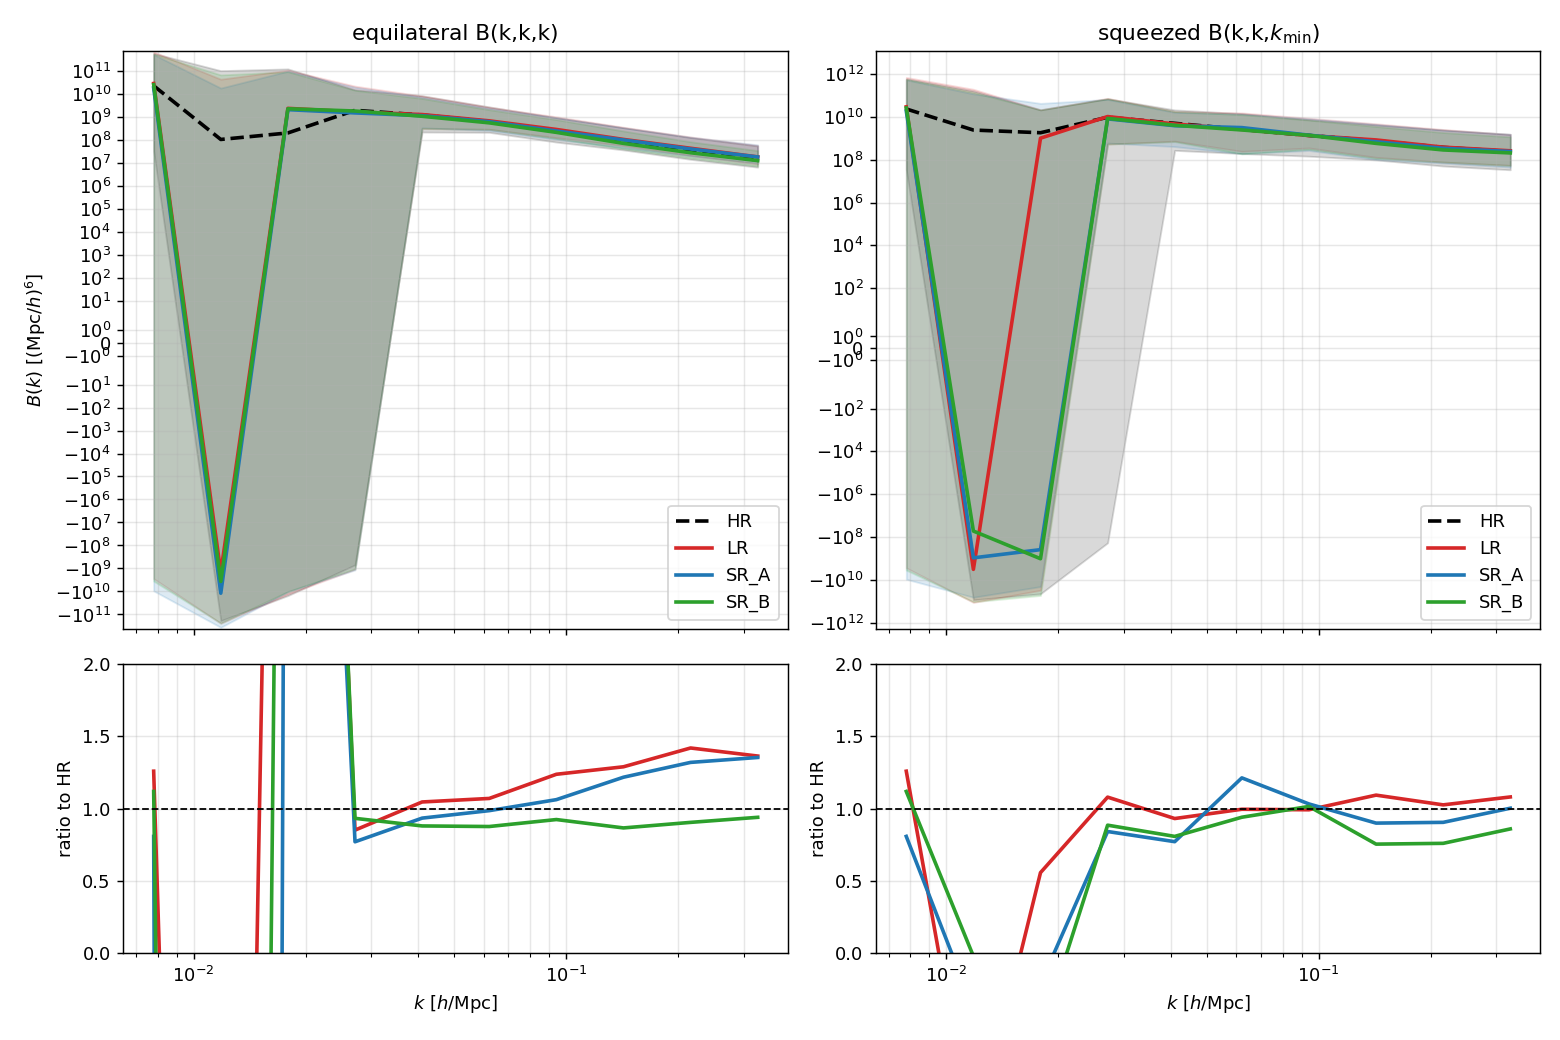
\includegraphics[width=0.95\linewidth]{figures_cmass/bispectrum_hr_lr_srA_srB.png}
\caption{Bispectrum of HR, LR, and SR (both arms), on $16$ test boxes. Top:
equilateral and squeezed bispectrum, HR in black. Bottom: ratio to HR. SR
removes most of the systematic excess that LR has at the plotted scales,
without ever training on this statistic.}
\label{fig:srs-bispec}
\end{figure}

On the equilateral configuration, LR sits about $6$ to $13$ percent above HR
across the middle range of scales. SR removes most of this gap without ever
seeing a bispectrum during training, and it does this for both arms. This is
evidence that the model is not simply fitting the training metric. It is
correcting real structure in the field that also shows up in a statistic it
never saw. (The figure uses the earlier models trained \emph{with} the power
spectrum loss; the no-Pk models of the following paragraphs preserve the
bispectrum at least as well, so removing that loss did not degrade this
held-out statistic either.)

\paragraph{Removing the power spectrum loss.} Following the meeting, we
retrained the model with the power spectrum term switched off
($\lambda_\text{pk}{=}0$ in Eq.~\ref{eq:srs-lossG}), so the loss is only the
adversarial and $L_1$ terms. We also changed which checkpoint counts as "best"
to the real-space $L_1$ error, since selecting on the power spectrum would
have been the same kind of leak we were trying to remove.

\begin{figure}[t]
\centering
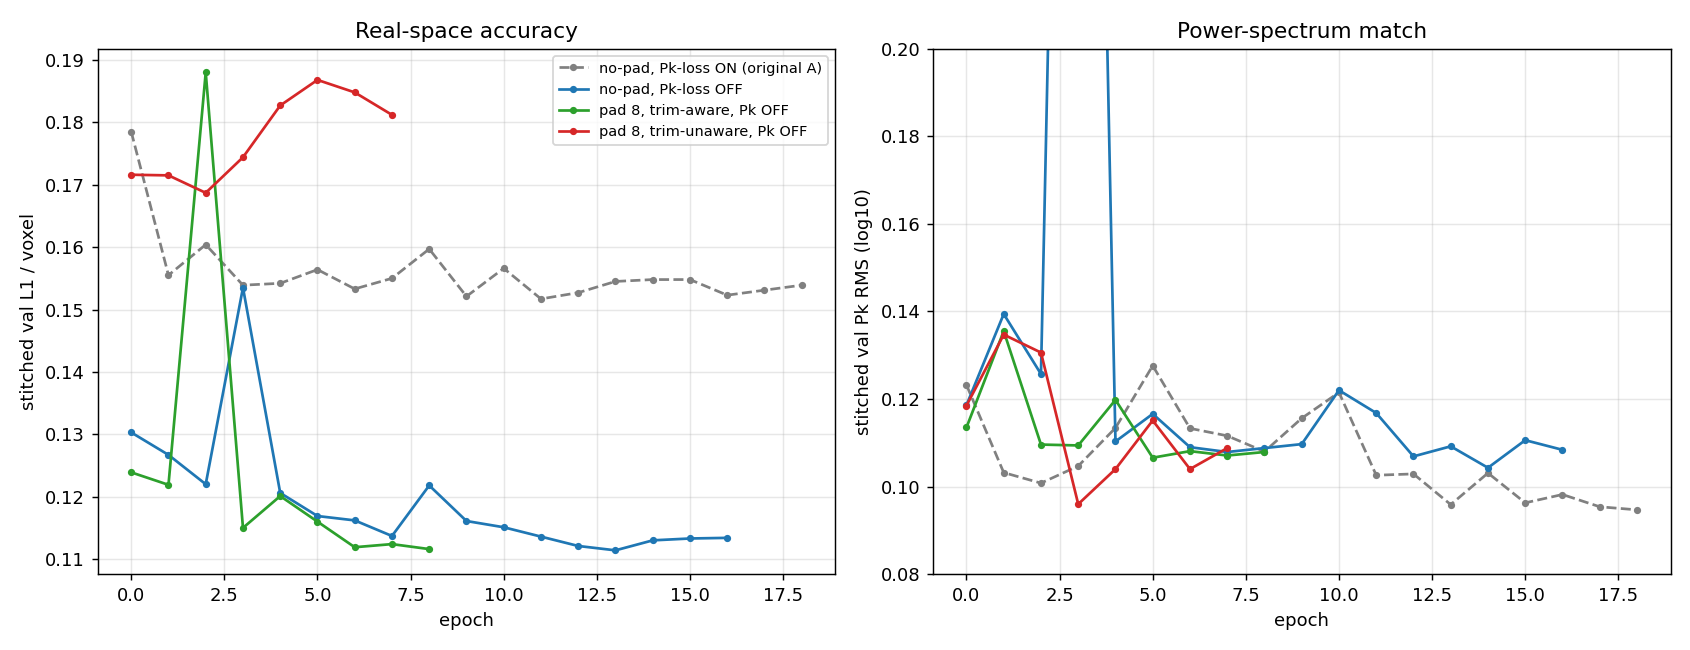
\includegraphics[width=0.98\linewidth]{figures_cmass/protocolv2_cmass.png}
\caption{Stitched validation curves under the new protocol (power spectrum
loss off). Left: real-space $L_1$ error. Right: power spectrum RMS error. Grey
dashed: the original Arm A with the power spectrum loss on, for comparison.
These runs are still training; curves stop at the most recent completed
epoch.}
\label{fig:srs-protocolv2}
\end{figure}

Two things stand out so far. First, without the power spectrum term, the
real-space $L_1$ error becomes clearly better than the original run at the
same point in training (left panel, blue and green curves sit below the grey
dashed curve). Second, the power spectrum error does get a little worse
without its loss term, but it does not collapse: it settles into roughly the
same range as before, just a bit noisier. So the power spectrum term was
buying us a small amount of power spectrum accuracy at a real cost in
real-space accuracy. It was not the only reason the power spectrum matched
well; the adversarial and reconstruction terms carry most of that on their
own.

\paragraph{Does padding help, once the power spectrum loss is out of the way?}
The report above found that padding (Arm B) did not beat no padding (Arm A) on
the power spectrum. The mentor pointed out two different ways this could
happen, and that they make different, testable predictions:
\begin{itemize}
  \item \textbf{Trim-aware.} The model is trained knowing that only the middle
  part of its output will be kept; the loss only looks at that middle part.
  This is what Arm B already did. If this is working correctly, padding should
  train at least as well as no padding, since it has strictly more context for
  the same target.
  \item \textbf{Trim-unaware.} The model is trained as if its whole padded
  output matters, including the edge region that gets thrown away later. If
  the model leans on that edge region during training, it should look fine
  during training but generalize worse once the edge is cut off at test time.
\end{itemize}
We trained both versions with the power spectrum loss off, so the comparison
is not confused by that term. Figure~\ref{fig:srs-protocolv2} shows all three
runs together (no padding, trim-aware padding, trim-unaware padding).

The trim-aware version (green) matches or beats no-padding (blue) on both
real-space error and power spectrum error at almost every epoch measured so
far. This supports the first prediction: once the model is told correctly what
part of its output is graded, more context helps rather than hurts. The
trim-unaware version (red) is clearly worse on real-space error than both
other runs, and does not close that gap as training continues. This supports
the second prediction: a model that is allowed to rely on the part of its
output that gets discarded at test time pays for that at test time. Put
together, the original result that padding did not help was most likely
caused by the power spectrum loss, not by padding itself.

We also reran the older, padding-with-power-spectrum-loss model for more
epochs to check whether it had simply not been trained long enough. Fifteen
additional epochs did not beat its early best score, so that run was not
undertrained; the training recipe, not the training time, was the limiting
factor.

\subsection{The Goal Metric: Corrected Cross-Fidelity Results}
\label{sec:srs-correction}

\paragraph{The bug.} After the analysis above, a routine physical sanity check
failed in a way that could not be real: the amplitude of the power spectrum had
essentially zero correlation with $\sigma_8$, and a fit of the power spectrum to
the five parameters explained only $0.2\%$ of the variance. The power spectrum
amplitude must scale with $\sigma_8$, so this pointed to a labeling error, not to
physics. Tracing it, we found that the processed count fields were written in
string-sorted simulation order ($0, 1, 10, 100, 1000, \dots$) while the cosmology
table is indexed numerically. Field number $k$ is therefore the halo field of
simulation string-sort$(k)$, not simulation $k$, so every field in the whole
pipeline was paired with the wrong cosmology. We proved this exactly: using the
original halo catalogs, the field halo count matches the catalog count under the
string-sort permutation for all $2000$ simulations, while the identity mapping
matches only the two fixed points. We corrected the cosmology table to field
order, backed up the old one, and patched the builder so it cannot regenerate the
wrong order.

\begin{figure}[h]
\centering
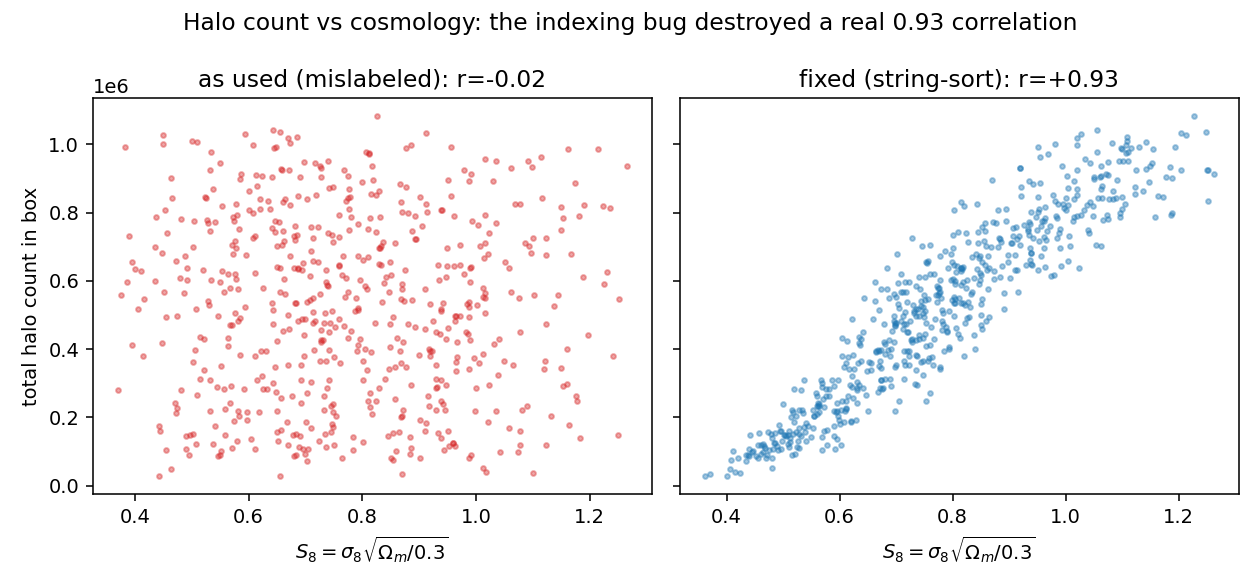
\includegraphics[width=0.85\linewidth]{figures_cmass/labelbug_count_vs_s8.png}
\caption{The indexing bug in one picture. Total halo count in a box against
$S_8 = \sigma_8\sqrt{\Omega_m/0.3}$. As the pipeline used the labels (left) the
correlation is zero; with the string-sort mapping corrected (right) the true
$0.93$ correlation reappears. Halo abundance must track $S_8$, so the left panel
was the signature of a labeling error, not of uninformative data.}
\label{fig:srs-labelbug}
\end{figure}

\paragraph{What this changes, and what it does not.} Every cosmology number we
computed before this point used the labels and is affected; the earlier
cross-fidelity tables have been removed and are replaced by the corrected results
below, and the earlier reading that the SR-versus-LR difference was an irreducible
coin flip was itself a product of the mislabeling. The results that do not use the
labels are unaffected and still stand: the power spectrum match of SR to HR, the
held-out bispectrum, the field-match statistics, the seam test, and the real space
error. The generator conditions on the cosmology as a style vector and was trained
with the scrambled labels, so its conditioning was uninformative during training;
we return to this at the end.

\paragraph{The data is informative after all.} With correct labels the picture
inverts. A halo count in this suite carries a strong cosmological signal: the
total halo count alone correlates with the combination $S_8 = \sigma_8
\sqrt{\Omega_m/0.3}$ at $0.93$ and with $\Omega_m$ at $0.85$. A Fisher forecast on
a single-box power spectrum now explains $98\%$ of the variance, where it
explained $0.2\%$ before, and it constrains $\Omega_m$ and $\sigma_8$ well, with
$\Omega_b$, $h$ and $n_s$ weak or unconstrained, which is the textbook pattern for
a low-redshift halo field. The field-level network tells the same story: after the
fix its predicted $\Omega_m$ correlates with the truth at $0.90$ on both training
and test boxes, where before the fix the correlation was zero and the output was a
constant. So the earlier conclusion that a single box carries almost no cosmology
was an artifact of the labeling, not a property of the data.

\begin{figure}[h]
\centering
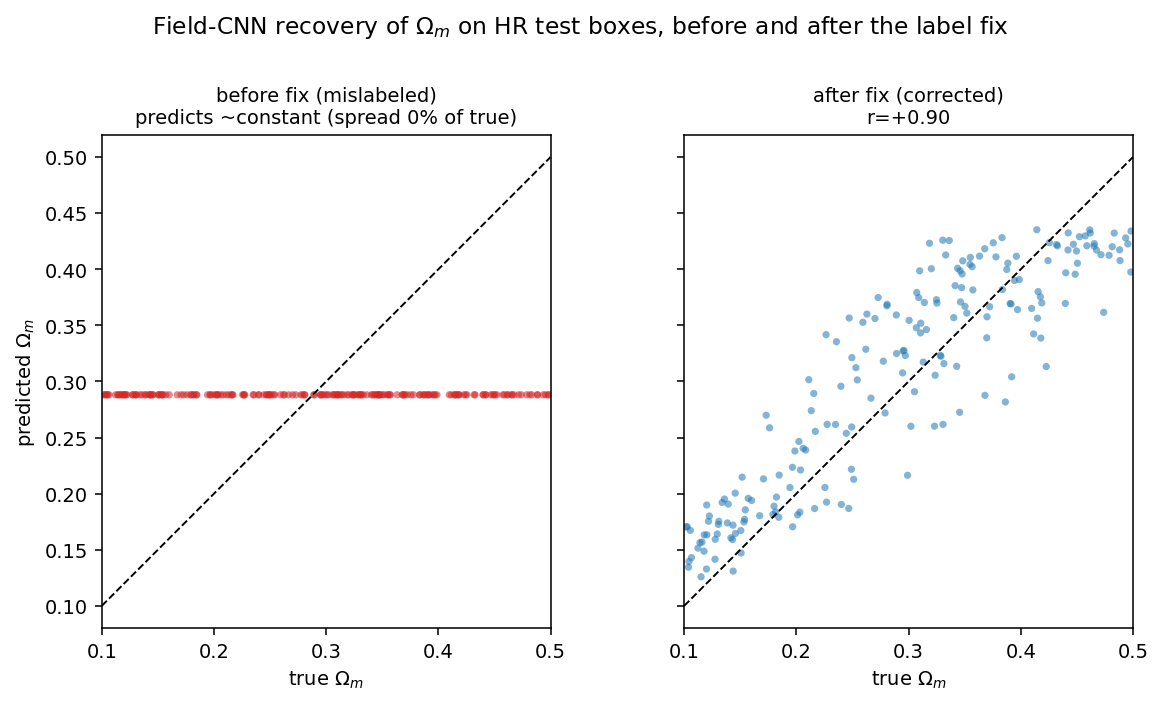
\includegraphics[width=0.82\linewidth]{figures_cmass/field_recovery_Om_cmass.png}
\caption{Field-level CNN recovery of $\Omega_m$ on HR test boxes, before and after
the label fix. Before (left) the prediction is flat and uncorrelated with the
truth (the network returns a near-constant); after (right) it tracks the diagonal
at a correlation of about $0.90$, on both training and test boxes. Same
architecture, same data, only the labels changed.}
\label{fig:srs-recovery}
\end{figure}

\begin{figure}[h]
\centering
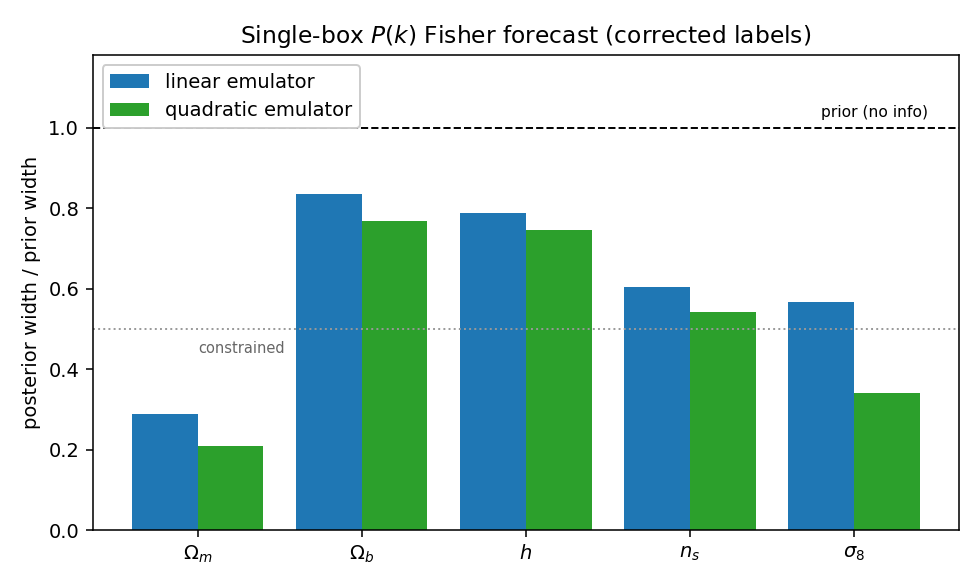
\includegraphics[width=0.72\linewidth]{figures_cmass/fisher_corrected_cmass.png}
\caption{Fisher forecast for a single-box power spectrum with corrected labels:
posterior width divided by prior width per parameter (lower means better
constrained, $1$ means no information). $\Omega_m$ is well constrained and
$\sigma_8$ is constrained, while $\Omega_b$, $h$ and $n_s$ are weak, the textbook
pattern for a low-redshift halo field. Two emulators (linear average slope and
quadratic at the prior centre) bracket the estimate.}
\label{fig:srs-fisher}
\end{figure}

\paragraph{Corrected cross-fidelity, and where SR helps.} We re-ran the goal
metric with correct labels at two levels, the power spectrum summary and the full
field. We train the posterior on one source, apply it to HR, and compare to a
posterior trained on HR, using an ensemble of independently retrained estimators
so the numbers are not single draws. Table~\ref{tab:srs-corrected} gives the
result.
\begin{table}[h]
\centering
\caption{Corrected cross-fidelity KL to HR (posterior trained on the named source,
evaluated on HR), lower is better, with the HR-to-HR floor for reference. Summary
uses the power spectrum; field uses a three-dimensional CNN posterior on the full
box.}
\label{tab:srs-corrected}
\begin{tabular}{lccc}
\toprule
level & LR (raw) & SR & HR floor \\
\midrule
summary $P(k)$ & $0.032$ & $0.088$ & $0.028$ \\
field (CNN)    & $0.49 \pm 0.81$ & $\mathbf{0.024}$ & $0.022$ \\
\bottomrule
\end{tabular}
\end{table}
\begin{figure}[h]
\centering
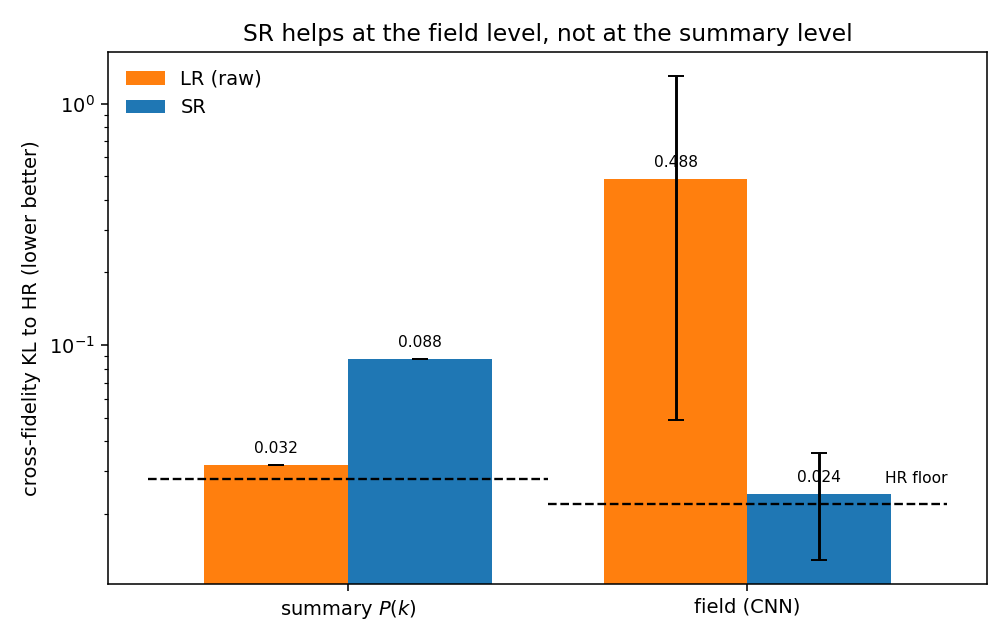
\includegraphics[width=0.7\linewidth]{figures_cmass/crossfid_corrected_cmass.png}
\caption{Corrected cross-fidelity KL to HR (log scale, lower is better) at the two
levels, with the HR-to-HR floor shown as the dashed line. At the summary level the
raw LR field is already at the floor and SR does not help. At the field level, an
LR-trained posterior does not transfer to HR (large and unstable), while an
SR-trained posterior sits at the floor. SR helps exactly where it corrects the
field.}
\label{fig:srs-crossfid-corrected}
\end{figure}
The two levels point in opposite directions, and both make sense. At the summary
level the raw LR power spectrum is already at the HR floor, so an LR-trained
posterior transfers to HR as well as an HR-trained one does, and there is no gap
for SR to close; SR even hurts a little, because the generator reshapes the
small-scale power in a way that does not match how HR responds to cosmology. At
the field level the raw LR box looks different enough from HR that an LR-trained
posterior does not transfer, and it does so unreliably, sometimes acceptably and
sometimes catastrophically, which is why its number carries such a large spread.
SR corrects the field to look like HR, so an SR-trained posterior transfers to HR
reliably, at the floor. This is exactly the deployment case the project is built
on, train the inference model on cheap SR-corrected boxes and apply it to
expensive HR, and at the field level SR makes it work where raw LR does not.

\paragraph{Padding on the goal metric.} We ran the two padding variants through
the corrected cross-fidelity at the summary level as well
(Table~\ref{tab:srs-padding}). Among the SR models the ordering from the earlier
report survives: no padding is best on the goal metric, trim-aware padding is
worse, and trim-unaware is worst, so for the cosmology objective the no-padding
model is the one to use. All three sit above the raw LR control at this level,
consistent with LR already being HR-like on the power spectrum. One number does
change under the fix: the mislabeled data made trim-unaware look catastrophic (a
factor of several hundred above the others), while with correct labels it is the
weakest variant by about a factor of two, not a blow-up. Its real-space error
(Figure~\ref{fig:srs-protocolv2}) remains the clearest and most direct sign that
it is the least reliable model.
\begin{table}[h]
\centering
\caption{Corrected cross-fidelity KL to HR at the summary (power spectrum) level
for the SR padding variants, with the LR control and the HR floor. Lower is
better. Field-level padding numbers are future work.}
\label{tab:srs-padding}
\begin{tabular}{lc}
\toprule
model & summary cross-fidelity KL \\
\midrule
SR, no padding & $\mathbf{0.087}$ \\
SR, trim-aware padding & $0.127$ \\
SR, trim-unaware padding & $0.172$ \\
\midrule
LR (control) & $0.031$ \\
HR floor & $0.028$ \\
\bottomrule
\end{tabular}
\end{table}

\paragraph{Bottom line.} With the labels fixed, the cosmology question has a
clear answer. The data constrains $\Omega_m$ and $\sigma_8$ from a single box. At
the power spectrum level the raw LR field is already HR-like, so SR is not needed
there and slightly hurts. At the field level, which is what SR actually corrects,
an SR-trained posterior transfers to HR at the floor while a raw LR one does not,
so SR provides a real and reliable cosmology benefit exactly where it operates.
Trim-unaware padding is still the weakest variant, worst on the goal metric and
on real-space error, though the label fix shrinks its apparent failure from
catastrophic to about a factor of two. Two honest caveats remain: the
field-level LR number has a wide spread and rests on a handful of retrained
networks, so the size of the gap should be firmed up with more seeds; and because
the generator was trained with the scrambled labels, its cosmology conditioning
was uninformative, so a retrain with correct conditioning may sharpen the SR
result further. Neither caveat changes the direction: with correct labels, SR
helps cosmology at the field level.

\paragraph{A data reliability note.} Partway through these runs, the shared
data storage this project reads from filled up completely, which caused a few
training jobs to fail with a file briefly appearing missing even though it was
not actually deleted. We added a retry step to the data loader and resumed
each affected run from its last saved checkpoint, so no real training progress
was lost. This is a shared infrastructure issue, not a problem with the data or
the method.

\subsection{Files}
\begin{itemize}\itemsep0pt
  \item Data and patching: \texttt{data/patch\_dataset\_cmass.py}
  (shared ops in \texttt{data/patch\_dataset\_real.py})
  \item Model: \texttt{map2map/models/styled\_srsgan.py}
  (\texttt{G\_correct}, \texttt{D\_const})
  \item Training: \texttt{train\_patch\_cmass.py};
  run script \texttt{scripts/train\_patch\_cmass.slurm}
  \item Inference and stitching: \texttt{infer\_stitch\_cmass.py}
  \item Seam eval: \texttt{analysis/eval\_seam\_cmass.py}
  \item Box / per-patch diagnostics: \texttt{analysis/diag\_cmass.py}
  \item SR-vs-HR match stats: \texttt{analysis/match\_stats\_cmass.py}
  \item SR-vs-HR power-spectrum figure: \texttt{analysis/plot\_sr\_vs\_hr.py}
  \item Bispectrum (held-out statistic): \texttt{analysis/bispectrum\_cmass.py}
  \item Training loss curves: \texttt{analysis/plot\_losses\_cmass.py}
  \item Cross-fidelity posterior evaluation: \texttt{evaluate.py} (SR-trained
  or LR-trained posterior evaluated on HR $P(k)$)
  \item Protocol-v2 (no-Pk-loss, padding-variant) training curves:
  \texttt{analysis/plot\_protocolv2\_cmass.py}
  \item Power spectrum on counts: \texttt{analysis/power\_spectrum.py}
  (estimator \texttt{counts}); differentiable training version
  \texttt{analysis/pk\_torch.py}
  \item Posterior and KL: \texttt{inference/nde.py}, \texttt{evaluate.py};
  end-to-end eval \texttt{scripts/eval\_cmass\_wrapper.slurm}
  \item Field-level posterior (three-dimensional CNN, moment-network loss):
  \texttt{models/field\_cnn.py}, \texttt{train\_field\_cnn.py};
  SR field generation \texttt{gen\_sr\_fields.py}; capacity and recovery
  diagnostics \texttt{overfit\_test.py}, \texttt{field\_diag.py}
  \item Outputs: \texttt{runs/patch\_cmass/}; figures: \texttt{figures\_cmass/}
\end{itemize}
.
% Needs the packages main.tex already loads (booktabs, algorithm, algpseudocode,
% listings, xcolor, graphicx). Figures live in figures_cmass/.
% Numbers (updated 2026-09-28, see research_scratch_5.md): summary cross-fid from
% logs/3248394_seedxfid.log (nde_v2, 8 seeds for the main arms) and
% logs/3200801_seedxfid.log (4-seed ablation rows); field cross-fid from
% logs/3248260_fieldev.log (Flow+GAN, 40 epochs), logs/3203212_fieldev.log (20 epochs)
% and the other *_fieldev.log files; scale-by-scale from scratch/why/coh.py
% (COH_SPLIT=test, 200 test boxes); posterior shifts from scratch/why/post_diag_any.py
% (logs/3249151_postdiag.log, logs/3251464_postdiag.log); PQMass, bispectrum and halo
% counts from logs/*_tier1.log; calibration from logs/3251512_spread.log; figures from
% flow_matching/plot_sec7.py. LR here is CHARM (section6_srs.tex calls it FastPM,
% which is wrong).
% =====================================================================

\definecolor{ablgood}{HTML}{1B7F1B}
\newcommand{\abgood}[1]{\textcolor{ablgood}{\textbf{#1}}}

\section{Flow+GAN: Flow Matching Started from the GAN}
\label{sec:flowgan}

This section documents the third model in this work at the same level of detail
as \S\ref{sec:srs}. \S\ref{sec:srs} corrects the LR halo count field with a
styled GAN. The GAN makes the field look like HR, but it is deterministic, and
it biases the summary-level cosmology posterior. Here we keep that GAN and add a
conditional \textbf{flow-matching} model on top of it. The flow starts from the
GAN's output plus noise and learns to turn it into a sample of the HR field. We
call the combined model \textbf{Flow+GAN}. The section ends with a table of
every model and ablation we ran on this data (\S\ref{sec:flowgan-ablations}).

\paragraph{Goal.} The goal is the same as in \S\ref{sec:srs}. At inference the
model sees only the cheap LR field and must produce an SR field that behaves like
HR. We grade it the same way: a posterior trained on SR fields is applied to HR
fields, and we measure how far its answer is from a posterior trained on HR
(cross-fidelity KL). HR is used only for training and grading.

\paragraph{Why a new model: what the GAN and a plain flow get wrong.} Two
findings from the previous section and its follow-ups motivate this design.
\begin{itemize}
  \item \textbf{The GAN is deterministic and tilts the power spectrum.} Its
  learned noise strength is about $2\times10^{-4}$, so ten noise draws give the
  same field. Its $L_1$ term pulls each voxel toward the conditional median.
  This shrinks the large-scale contrast (about $5\%$ less power at $k<0.06\,h\,\mathrm{Mpc}^{-1}$)
  and adds $1$ to $3\%$ power at high $k$. A posterior reads this tilt as a
  shift in $\sigma_8$: on HR test boxes the GAN-trained posterior's $\sigma_8$ mean
  is off by about one HR posterior width. That is why the deployed GAN's summary
  cross-fidelity KL ($0.202$) is worse than raw LR ($0.049$). One fixed per-$k$
  calibration curve on the GAN's training $P(k)$ brings it to $0.068$, which
  shows the problem is this tilt, not missing information.
  \item \textbf{A plain flow samples, but loses the large scales.} A flow that
  starts from pure Gaussian noise (``Flow'' below) has no $\sigma_8$ bias and
  reaches $0.087$. But it rebuilds every scale from noise, including the largest
  ones, which LR already gets right. Its large-scale power scatters more from box
  to box than LR's. Its coherence with HR at $k\approx0.125$ falls below LR's.
  Its predictions are also too narrow: HR usually falls outside the spread of its
  draws (spread-skill ratio $0.20$, ideal $1$).
\end{itemize}
Flow+GAN takes the part each model gets right. The GAN supplies the large-scale
structure and a best guess. The flow adds only what the best guess cannot
predict, and it adds it as a sample, not as a mean. This follows residual
diffusion for downscaling (CorrDiff, Mardani et al.\ 2023, arXiv:2309.15214),
stochastic flow matching for super-resolution (Fotiadis et al.\ 2024,
arXiv:2410.19814), and stochastic interpolants with a data-dependent start
(Albergo et al.\ 2023, arXiv:2310.03725).

\paragraph{Terminology.} \textbf{GAN} means the deployed generator of
\S\ref{sec:srs}: Arm A (pad $0$), power-spectrum loss off, trained with correct
cosmology labels, run at the fiducial cosmology (tag \texttt{Afixfid}).
\textbf{Flow} means the pure-noise flow matcher trained on $64^3$ patches (tag
\texttt{fm\_gauss\_nodq}). \textbf{Flow+GAN} is the model of this section. As in
\S\ref{sec:srs}, we use LR/LF and HR/HF interchangeably.

\subsection{Data Preprocessing}
\textit{Source: \texttt{cmass-ili}; loaders \texttt{flow\_matching/data.py}
(\texttt{FullBoxDataset}), model space \texttt{flow\_matching/space.py}.}

\paragraph{Input.} The data is the same as in \S\ref{sec:srs}: $2000$ paired
halo count grids of $128^3$ cells on a periodic $1000\,h^{-1}\mathrm{Mpc}$ box at
$z=0.5$, with LR from CHARM and HR from Quijote N-body, and the same
$1600/200/200$ train/validation/test split. One extra input is new. Before
training, we run the GAN once on every one of the $2000$ LR boxes, at the
fiducial cosmology, and store its output (\texttt{sr\_fields/Afix\_fiducial}).
The GAN is frozen from here on; it is not trained further.

\paragraph{Model space.} The flow works on a standardised log count,
\begin{equation}
  y = \frac{\log(1+n) - \mu}{s}, \qquad
  n = \mathrm{round}\big(\exp(s\,y+\mu) - 1\big) \ \ \text{clamped to } [0, 200],
  \label{eq:fg-space}
\end{equation}
where $\mu=0.152$ and $s=0.359$ are the mean and standard deviation of
$\log(1+n_\text{HR})$ over $50$ training boxes. The LR field, the GAN field and
the HR target all use this same map. We do \emph{not} dequantise (add uniform
noise to the integer counts before the log). An earlier flow that did so
(\texttt{fm\_gauss}) needed a floor decoder, and noise near the empty-cell
boundary made spurious halos: about $9\%$ too many halos, and a summary KL of
$0.244$. The rounding decoder in Eq.~\ref{eq:fg-space} does not have this bias.
Power spectra are computed exactly as in \S\ref{sec:srs}, on the physical-count
overdensity $\delta = n/\bar n - 1$ with the per-box mean.

\subsection{Data Pipeline (full box, no patches)}
\textit{Located in: \texttt{flow\_matching/data.py},
\texttt{flow\_matching/augment.py}, \texttt{flow\_matching/train\_fm.py}.}

Unlike the GAN and the earlier flows, Flow+GAN is trained and sampled on the
\textbf{whole $128^3$ box at once}. The patch pipeline of \S\ref{sec:srs} cuts
each box into eight $64^3$ cores. For a model that draws fresh noise per patch,
this matters: each patch gets its own noise. Modes longer than a patch are then
re-drawn independently in each patch, and the circular padding treats a patch as
periodic when it is not. Sampling the old patch-trained flow on the full box
already raised its coherence with HR at $k=0.125$ from $0.36$ to $0.67$. The
velocity network is fully convolutional with circular padding, so it runs on
$128^3$ without change, and the box is truly periodic, so circular padding is
exact.

Each training item is one box: the LR counts, the HR counts and the GAN output,
all $128^3$. Two augmentations are applied identically to all three fields:
\begin{itemize}
  \item \textbf{Random periodic shift.} The three fields are rolled by the same
  random offset along each axis. Because the box is periodic this is an exact
  symmetry, and it stops the network from learning fixed positions.
  \item \textbf{Cube symmetries.} One of the $48$ rotations and reflections of
  the cube (\texttt{--aug full48}).
\end{itemize}

\begin{table}[t]
\centering
\caption{Notation for the Flow+GAN pipeline.}
\label{tab:fg-notation}
\begin{tabular}{llp{7.0cm}}
\toprule
Symbol & Value & Meaning \\
\midrule
$N$ & $128$ & box side in voxels (the model sees the whole box) \\
$y_\text{LR},\,y_\text{GAN},\,y_\text{HR}$ & $(1,128^3)$ & LR, GAN and HR fields in model space (Eq.~\ref{eq:fg-space}) \\
$\sigma_z$ & $0.920$ & RMS of $y_\text{HR}-y_\text{GAN}$ over $50$ training boxes ($64^3$ patches) \\
$t$ & $[0,1]$ & flow time; $t{=}0$ is the noisy GAN field, $t{=}1$ is HR \\
$x_t$ & $(1,128^3)$ & point on the straight path between source and target \\
$v_\phi$ & $17.4$M params & velocity network (3D UNet) \\
\bottomrule
\end{tabular}
\end{table}

\subsection{Model: Input/Output Specification}
\textit{Implementation: \texttt{flow\_matching/interpolant.py}
(\texttt{Interpolant}, source \texttt{gan\_white}),
\texttt{flow\_matching/unet3d.py}.}

\paragraph{The path.} Flow matching learns a velocity field that carries a
\emph{source} sample $x_0$ to a \emph{target} sample $x_1$ along a straight line.
For Flow+GAN the source is the GAN's field plus white noise at the size of the
GAN's typical error, and the target is HR:
\begin{equation}
  x_0 = y_\text{GAN} + \sigma_z\,\boldsymbol\epsilon,\quad
  \boldsymbol\epsilon\sim\mathcal N(0,I), \qquad
  x_1 = y_\text{HR}, \qquad
  x_t = (1-t)\,x_0 + t\,x_1 .
  \label{eq:fg-path}
\end{equation}
The velocity along this line is constant, $x_1-x_0$. The network is trained to
predict it:
\begin{equation}
  \mathcal L_\text{FM} \;=\; \mathbb E_{t,\,\boldsymbol\epsilon,\,\text{box}}
    \big\lVert v_\phi\big(x_t,\,t,\,[y_\text{LR},\,y_\text{GAN}]\big) - (x_1 - x_0)\big\rVert_2^2 ,
  \qquad t\sim\mathcal U[0,1].
  \label{eq:fg-loss}
\end{equation}
This is the only loss. There is no adversarial term, no $L_1$ term and no
power-spectrum term.

\paragraph{Why start from the GAN.} With a pure-noise source ($x_0\sim\mathcal
N(0,I)$) the flow must create every scale, including the large scales that LR
and the GAN already get right. Starting at the GAN field means the flow's job is
only the residual $y_\text{HR}-y_\text{GAN}$, whose size is $\sigma_z$. The noise
$\sigma_z\boldsymbol\epsilon$ is what makes the model stochastic: with
$\sigma_z=0$ the flow would be a deterministic map and could return only one
field per LR box, which is the GAN's failure again. The noise is white, so it
has little power at large scales, and the large-scale modes of the start point
are essentially the GAN's.

\paragraph{Conditioning.} The network sees the current state $x_t$ and two
conditioning channels, the LR field and the GAN field, concatenated as input
channels ($3$ input channels in total). It does \emph{not} see the cosmology
vector: the flow is $\theta$-independent. The only $\theta$ in the pipeline is
the fixed fiducial value given to the frozen GAN, so no per-box cosmology can
leak into the SR fields.

\begin{table}[t]
\centering
\caption{Tensors consumed/produced by the velocity network for one box (batch
dimension omitted).}
\label{tab:fg-io}
\begin{tabular}{lll}
\toprule
Symbol & Shape & Meaning \\
\midrule
$x_t$ & $(1,128,128,128)$ & current state on the path (Eq.~\ref{eq:fg-path}) \\
$y_\text{LR}$ & $(1,128,128,128)$ & LR field, model space (conditioning) \\
$y_\text{GAN}$ & $(1,128,128,128)$ & frozen GAN output, model space (conditioning and start point) \\
$t$ & scalar & flow time, sinusoidal embedding \\
$v_\phi(\cdot)$ & $(1,128,128,128)$ & predicted velocity \\
\bottomrule
\end{tabular}
\end{table}

\paragraph{Velocity network.} $v_\phi$ is a 3D UNet with $17.4$M parameters.
\begin{enumerate}
  \item Every convolution is $3{\times}3{\times}3$ with circular padding, so the
  network is exactly shift-equivariant on the periodic box.
  \item Four levels at full, $1/2$, $1/4$ and $1/8$ resolution with channel
  widths $32\cdot(1,2,4,4)$, two residual blocks per level, GroupNorm, and one
  self-attention block at the coarsest level for global context.
  \item The time $t$ enters through a sinusoidal embedding and an MLP that sets a
  per-channel scale and shift after each GroupNorm (FiLM).
  \item The last convolution is initialised to zero, so the initial velocity is
  about $0$.
\end{enumerate}
Training keeps an exponential moving average (EMA, decay $0.999$) of the weights;
validation and sampling use the EMA weights.

\subsection{Training Step}
\textit{Located in: \texttt{flow\_matching/train\_fm.py}.}

\begin{algorithm}[H]
\caption{Flow+GAN training step (one box)}
\label{alg:fg-train}
\begin{algorithmic}[1]
\Require LR counts $\mathbf L$, HR counts $\mathbf H$, frozen GAN output $\mathbf G$ (all $128^3$), $\sigma_z$
\State draw one random periodic shift and one of $48$ cube symmetries; apply both to $\mathbf L,\mathbf H,\mathbf G$
\State $y_\text{LR},y_\text{HR},y_\text{GAN}\gets$ Eq.~\ref{eq:fg-space} applied to $\mathbf L,\mathbf H,\mathbf G$
\State $\boldsymbol\epsilon\sim\mathcal N(0,I)$, \ $t\sim\mathcal U[0,1]$
\State $x_0\gets y_\text{GAN}+\sigma_z\boldsymbol\epsilon$, \ $x_t\gets(1-t)x_0+t\,y_\text{HR}$
\State $\mathcal L\gets\big\lVert v_\phi(x_t,t,[y_\text{LR},y_\text{GAN}])-(y_\text{HR}-x_0)\big\rVert^2$ \Comment{mean over voxels}
\State update $\phi$ (AdamW, linear warm-up $500$ steps, grad-clip $1$, bf16); update EMA
\end{algorithmic}
\end{algorithm}

\paragraph{Validation and checkpoint selection.} After each epoch we generate
$2$ draws for each of the first $16$ validation boxes ($16$ Heun steps) and
compute, in $\log(1+n)$ space: the $L_1$ error per voxel, the fair
\textbf{CRPS} of the $2$-draw ensemble, the spread between draws, the
total-count error, and the $P(k)$ RMS against HR. For $K$ draws $s_1,\dots,s_K$
and the true value $h$, the per-voxel fair CRPS is
\begin{equation}
  \mathrm{CRPS} = \frac1K\sum_{i}|s_i-h| - \frac{1}{2K(K-1)}\sum_{i\neq j}|s_i-s_j| .
  \label{eq:fg-crps}
\end{equation}
The first term rewards draws close to HR; the second rewards draws that differ
from each other. So CRPS, unlike $L_1$, does not favour a blurred mean field.
\texttt{best.pt} is the epoch with the lowest validation CRPS. We fixed this rule
before training. $P(k)$ is only a check: it is never trained on and never used
to select.

\subsection{Inference}
\textit{Located in: \texttt{flow\_matching/sample\_fm.py},
\texttt{flow\_matching/common.py} (\texttt{generate\_box}).}

For one box: run the frozen GAN on LR (already stored), build the start point
$x_0$, integrate the learned velocity from $t=0$ to $t=1$ with Heun's
second-order method, and map back to counts. The noise is seeded by the box index
and draw number, so every output can be reproduced.

\begin{algorithm}[H]
\caption{Flow+GAN inference (one box, one draw)}
\label{alg:fg-infer}
\begin{algorithmic}[1]
\Require LR box $\mathbf L$, GAN output $\mathbf G$, trained $v_\phi$ (EMA), $\sigma_z$, steps $S{=}32$, seed
\State $y_\text{LR},y_\text{GAN}\gets$ Eq.~\ref{eq:fg-space}; \ $x\gets y_\text{GAN}+\sigma_z\boldsymbol\epsilon$ \Comment{seeded $\boldsymbol\epsilon$}
\For{$i=0,\dots,S-1$} \Comment{$t_i=i/S$, $\Delta t = 1/S$}
  \State $v_0\gets v_\phi(x,t_i,[y_\text{LR},y_\text{GAN}])$
  \If{$i<S-1$}
    \State $v_1\gets v_\phi(x+\Delta t\,v_0,\,t_{i+1},[y_\text{LR},y_\text{GAN}])$; \ $x\gets x+\tfrac12\Delta t\,(v_0+v_1)$ \Comment{Heun}
  \Else
    \State $x\gets x+\Delta t\,v_0$ \Comment{Euler on the last step}
  \EndIf
\EndFor
\State \Return $\mathrm{round}\big(\exp(s\,x+\mu)-1\big)$, clamped to $[0,200]$ \Comment{integer counts}
\end{algorithmic}
\end{algorithm}

\paragraph{No stitching.} Because the whole box is generated at once, there are
no cores, no halo and no seams. The stitching step of \S\ref{sec:srs} does not
apply.

\subsection{Evaluation}
\label{sec:fg-eval}
\textit{Located in: \texttt{evaluate.py}, \texttt{inference/nde.py},
\texttt{analysis/seed\_xfid\_check.py}, \texttt{eval\_field\_crossfid.py},
\texttt{scratch/why/coh.py}, \texttt{flow\_matching/plot\_sec7.py}.}

We use the metrics of \S\ref{sec:srs-eval}: the power spectrum, the transfer
$T(k)=P_X/P_\text{HR}$, the cross-coherence $r(k)$ with HR
(Eq.~\ref{eq:srs-Tr}), and cross-fidelity KL (Eq.~\ref{eq:srs-kl}) at two levels.
One thing changed in the summary-level protocol, so the numbers below are not
directly comparable to Table~\ref{tab:srs-corrected}:
\begin{itemize}
  \item \textbf{Summary level (protocol v2).} The NDE input is $\log_{10}P(k)$ in
  $29$ bins. The three lowest of the original $32$ bins contain no Fourier modes,
  and we now drop them. We train $8$ NDE seeds for each of the main sources (HR,
  LR, GAN, Flow and every Flow+GAN checkpoint) and $4$ for the other ablations.
  For seed $s$ we compare $q_X^{(s)}$ with $q_\text{HR}^{(s)}$ on the $200$ HR test
  boxes and report the mean $\pm$ standard deviation over seeds. The HR floor is
  the KL between independently trained HR posteriors. This per-seed protocol is
  stricter than the ensemble protocol of \S\ref{sec:srs-correction}: LR is $0.049$
  here versus $0.032$ there. The ranking of the GAN arms is the same under both.
  \item \textbf{Field level.} Unchanged from \S\ref{sec:srs-correction}: a 3D CNN
  posterior on the full box, $3$ CNN seeds trained on SR, evaluated on HR test
  boxes against $6$ HR-trained reference CNNs. The same $8$ LR CNNs and $6$ HR
  CNNs are reused for every arm.
\end{itemize}

\subsection{Best-Run Configuration}
\textit{Run script: \texttt{scratch/why/train\_v2\_1gpu.slurm} (resumes automatically
from \texttt{last.pt}, so the same script ran epochs $0$ to $19$ and $20$ to $39$); checkpoint
\texttt{models/Flow+GAN/best\_crps40\_epoch39.pt}; sampling \texttt{scratch/why/gen\_v2.slurm}.}

\begin{lstlisting}[language=bash]
--source gan_white                        # python -m flow_matching.train_fm
--extra-dir sr_fields/Afix_fiducial     # frozen GAN output: start point + 2nd cond channel
--full-box --roll --aug full48          # whole periodic box, random shift + 48 symmetries
--no-dequant                            # round decoder
--base-ch 32 --ch-mult 1,2,4,4 --attn-levels 3    # 17.4M-param UNet
--lr 1e-4 --warmup 500 --ema 0.999 --grad-clip 1.0 --amp bf16
--epochs 40 --select crps --val-max-sims 16 --val-draws 2 --val-steps 16
# sampling: --steps 32 --method heun (full box, EMA weights, seeded per box)
\end{lstlisting}

The run used one GH200 GPU (about $13.5$ minutes per epoch, batch of one box).
Epochs are numbered from $0$, as in the training log. We first stopped the run
after $20$ epochs, because validation CRPS had been flat since epoch $11$; that
run's CRPS-best checkpoint was epoch $15$. The validation $P(k)$ error was still
falling, so we resumed the same run, with the same recipe, weights, EMA and optimizer state,
to the planned $40$ epochs. Before looking at any test result we fixed which
checkpoints to report: the CRPS-best one (epoch $38$, the one we use below) and the
final one (epoch $39$). Validation at those epochs:

\begin{center}
\begin{tabular}{lccccc}
\toprule
model & $L_1$/voxel & CRPS & spread & count error & $P(k)$ RMS \\
\midrule
Flow+GAN, epoch 15 (first $20$ epochs) & $0.146$ & $0.0749$ & $0.071$ & $+0.2\%$ & $0.059$ \\
Flow+GAN, epoch 38 (CRPS-best of $40$) & $0.144$ & $\mathbf{0.0740}$ & $0.070$ & $-1.6\%$ & $\mathbf{0.052}$ \\
Flow+GAN, epoch 39 (final) & $0.143$ & $\mathbf{0.0740}$ & $0.069$ & $-1.5\%$ & $0.053$ \\
Flow from noise, full box (control) & $0.195$ & $0.100$ & -- & $+3.2\%$ & $0.084$ \\
\bottomrule
\end{tabular}
\end{center}
The control row is the same recipe with a pure-noise source instead of the GAN,
read at epoch $7$ to $8$ for comparison (its later epochs were unstable). Flow+GAN
is better on every validation metric. The second $20$ epochs improve CRPS only
slightly ($0.0749\to0.0740$, flat from epoch $30$), but they reduce the $P(k)$ error
($0.059\to0.052$), even though $P(k)$ is not in the loss. The validation count error
is measured on only $16$ boxes and moves by about $1\%$ from epoch to epoch.

\subsection{Results}
\label{sec:fg-results}

\paragraph{1. Power spectrum: the tilt is gone.} Figure~\ref{fig:fg-pk} and
Table~\ref{tab:fg-scale} compare the power spectrum and cross-coherence of LR,
the GAN, the Flow and Flow+GAN against HR. Flow+GAN's median power is within
$1.4\%$ of HR at every scale ($0.986$ to $1.009$). The median transfer deviates
from $1$ by $1.1\%$ RMS, against $2.7\%$ for raw LR, $4.4\%$ for the GAN and
$6.1\%$ for the Flow. The GAN's pattern (too little power at large scales, too
much at small scales) is removed, and so is the Flow's $3$ to $4\%$ deficit at
most scales. The cross-coherence with HR is above LR at every scale except the
largest ($r=0.76$ vs $0.51$ at $k\approx0.125$, $0.34$ vs $-0.13$ at
$k\approx0.35$). It stays below the GAN's, which is expected: a sampler draws
the unpredictable small-scale structure fresh, while the GAN returns its
single best guess.

\begin{figure}[t]
\centering
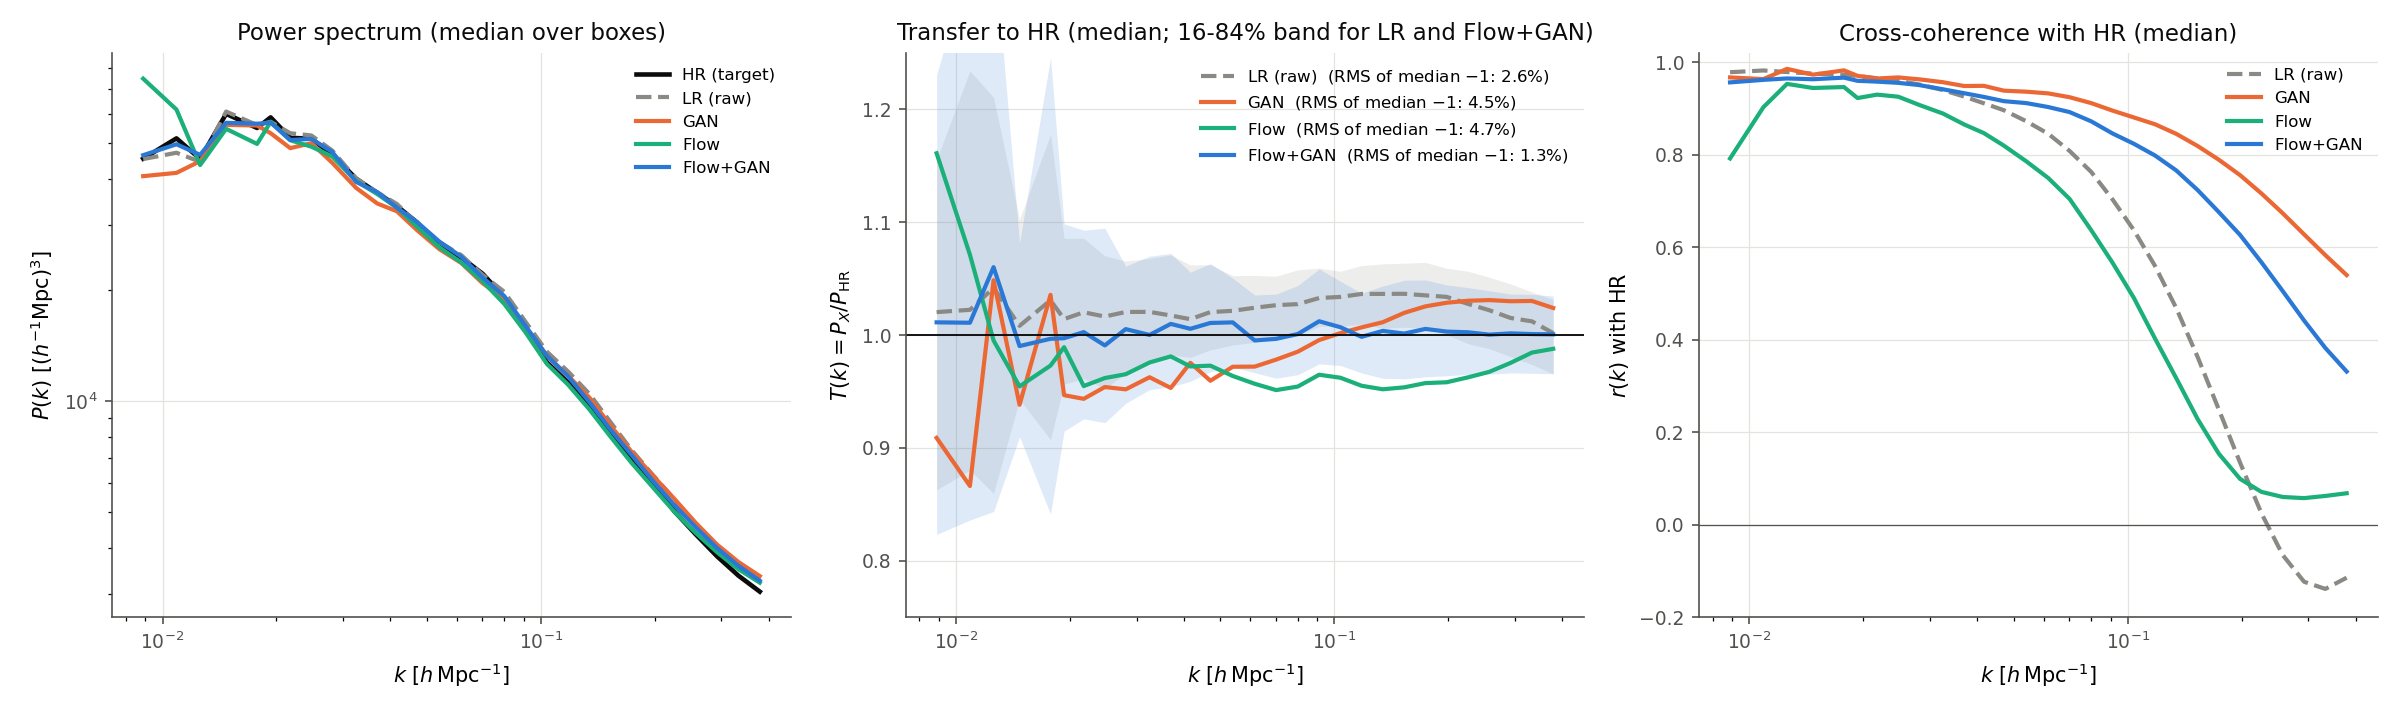
\includegraphics[width=\linewidth]{figures_cmass/pk_panel_box_flowgan.png}
\caption{Full-box diagnostic on $100$ validation boxes. Flow+GAN has no
test-split fields yet, and the first $16$ validation boxes (in sorted order)
were used for checkpoint selection, so we use the next $100$.
\textbf{Left:} median $P(k)$ of HR, LR, GAN, Flow and Flow+GAN.
\textbf{Middle:} transfer $T(k)=P_X/P_\text{HR}$, median, with the 16 to 84
percentile band for LR and Flow+GAN; the legend gives the RMS deviation of the
median from $1$. The GAN (orange) is low at large scales and high at small
scales; the Flow (green) is low at all scales; Flow+GAN (blue) stays on $1$.
\textbf{Right:} cross-coherence $r(k)$ with HR. Flow+GAN is above LR from
$k\approx0.05$ onward and below the deterministic GAN.}
\label{fig:fg-pk}
\end{figure}

\begin{table}[t]
\centering
\caption{Scale by scale, the first $100$ validation boxes, in wide $k$ bands
centred on the listed values. $P/P_\text{HR}$: median power
ratio to HR ($1$ is right). Scatter: box-to-box standard deviation of that ratio
(LR is the reference). $r$: median cross-coherence with HR ($1$ is best).}
\label{tab:fg-scale}
\small
\begin{tabular}{l cccc cc cccc}
\toprule
 & \multicolumn{4}{c}{$P/P_\text{HR}$ median} & \multicolumn{2}{c}{scatter} & \multicolumn{4}{c}{$r$ with HR} \\
\cmidrule(lr){2-5}\cmidrule(lr){6-7}\cmidrule(lr){8-11}
$k$ [$h\,\mathrm{Mpc}^{-1}$] & $0.013$ & $0.042$ & $0.125$ & $0.35$ & $0.013$ & $0.125$ & $0.013$ & $0.042$ & $0.125$ & $0.35$ \\
\midrule
LR (raw)  & $1.009$ & $1.017$ & $1.037$ & $1.007$ & $\mathbf{0.20}$ & $0.34$ & $\mathbf{0.975}$ & $0.908$ & $0.508$ & $-0.126$ \\
GAN       & $0.949$ & $0.962$ & $1.010$ & $1.029$ & $\mathbf{0.20}$ & $0.34$ & $0.974$ & $\mathbf{0.944}$ & $\mathbf{0.850}$ & $\mathbf{0.559}$ \\
Flow      & $1.057$ & $0.970$ & $0.959$ & $0.989$ & $0.40$ & $\mathbf{0.32}$ & $0.907$ & $0.837$ & $0.358$ & $0.062$ \\
Flow+GAN  & $\mathbf{0.986}$ & $\mathbf{1.004}$ & $\mathbf{0.998}$ & $\mathbf{1.009}$ & $0.29$ & $0.35$ & $0.964$ & $0.921$ & $0.760$ & $0.339$ \\
\bottomrule
\end{tabular}
\end{table}

\paragraph{2. Cross-fidelity: Flow+GAN matches LR at the summary level and stays near the floor at the field level.}
Figure~\ref{fig:fg-crossfid} and Table~\ref{tab:fg-crossfid} give the goal
metric. At the summary level the $40$-epoch Flow+GAN reaches $0.047\pm0.008$,
against $0.049\pm0.010$ for raw LR. Compared seed by seed (same NDE seed, same HR
reference posterior), the difference from LR averages $-0.001$. It is the first
SR model that is not worse than LR at the summary level: the GAN is at $0.202$
and the Flow at $0.087$. The final checkpoint (epoch $39$) gives $0.055\pm0.011$,
also equal to LR within noise. At the field level Flow+GAN reaches $0.027\pm0.011$,
close to the HR floor ($0.019$), while the LR-trained CNN posterior does not
transfer reliably ($0.47\pm0.78$).

Two cautions apply. First, epochs $38$ and $39$ are neighbouring checkpoints of one
run, yet their summary KLs differ by $0.008$, about one seed standard deviation.
So the fair claim is that Flow+GAN is equal to LR within noise, not that it beats
LR. Second, the $20$-epoch model (epoch $15$) was at $0.065\pm0.011$. The
improvement from longer training is therefore real but modest, and it is of the
same order as the checkpoint-to-checkpoint noise.

\begin{figure}[t]
\centering
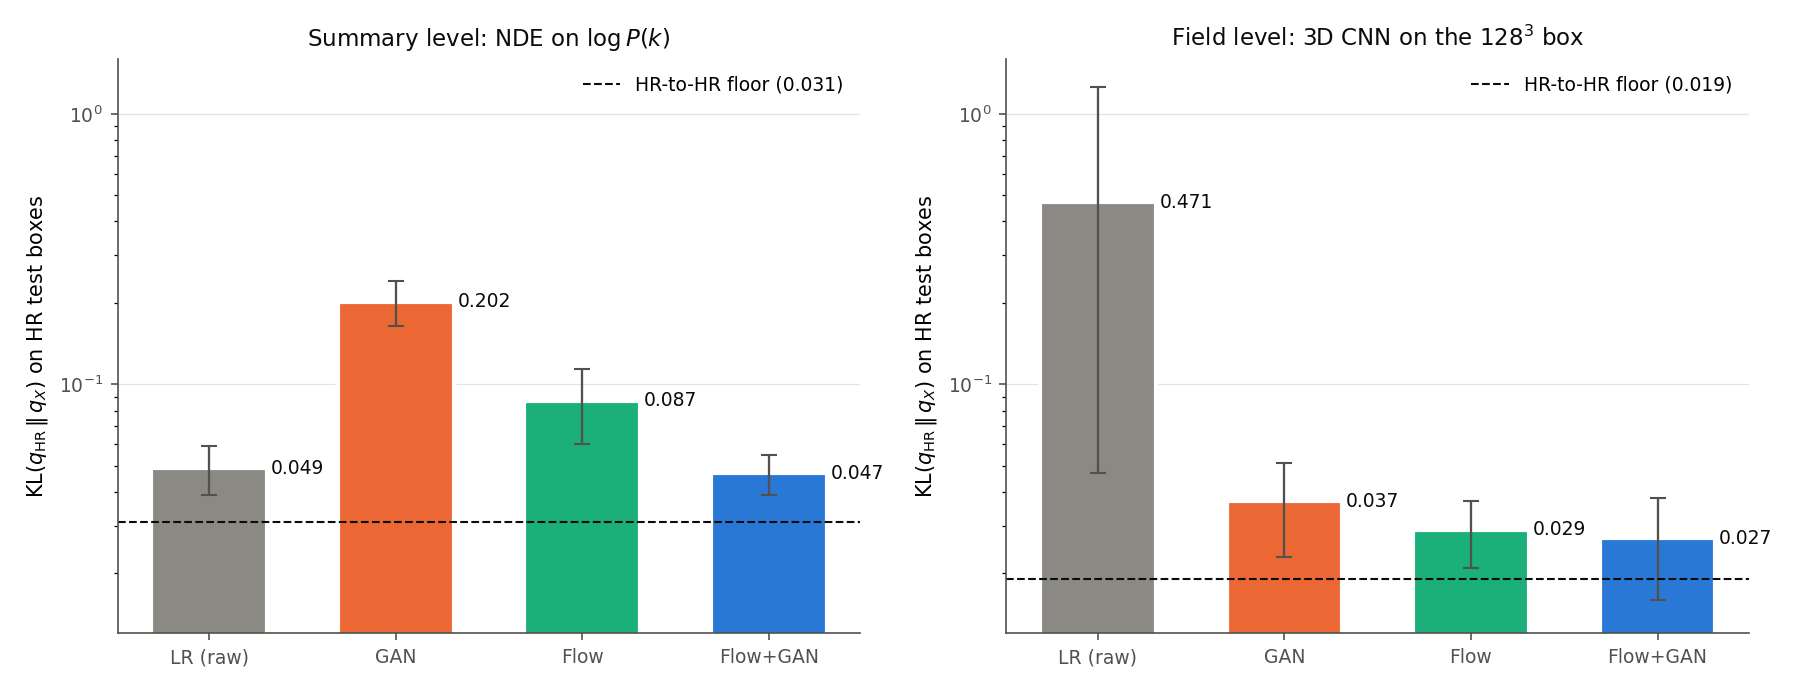
\includegraphics[width=0.95\linewidth]{figures_cmass/crossfid_flowgan.png}
\caption{Cross-fidelity KL to HR (log scale, lower is better), posterior trained
on source $X$ and applied to the $200$ HR test boxes. Dashed: HR-to-HR floor.
Flow+GAN is the $40$-epoch model (CRPS-best checkpoint).
\textbf{Left:} summary level ($P(k)$ NDE, protocol v2, mean $\pm$ std over $8$
seeds). Flow+GAN ($0.047$) equals raw LR ($0.049$); the GAN is at $0.202$ and the
Flow at $0.087$. \textbf{Right:} field level (3D CNN). All three SR models are
near the floor, Flow+GAN ($0.027$) closest; LR does not transfer reliably.}
\label{fig:fg-crossfid}
\end{figure}

\begin{table}[t]
\centering
\caption{Cross-fidelity KL to HR, lower is better. Summary: protocol v2, mean
$\pm$ std over $8$ NDE seeds, $200$ HR test boxes. Field: mean $\pm$ std over
HR-reference $\times$ SR-replicate pairs. Best SR value per column in bold.}
\label{tab:fg-crossfid}
\begin{tabular}{lcc}
\toprule
source & summary $P(k)$ & field (CNN) \\
\midrule
LR (raw, control) & $0.049\pm0.010$ & $0.471\pm0.782$ \\
GAN (deployed)    & $0.202\pm0.038$ & $0.037\pm0.014$ \\
Flow (noise start, patches) & $0.087\pm0.027$ & $0.029\pm0.008$ \\
Flow+GAN, epoch 15 ($20$-epoch run) & $0.065\pm0.011$ & $\mathbf{0.024\pm0.009}$ \\
Flow+GAN, epoch 38 (CRPS-best of $40$) & $\mathbf{0.047\pm0.008}$ & $0.027\pm0.011$ \\
Flow+GAN, epoch 39 (final) & $0.055\pm0.011$ & $0.027\pm0.015$ \\
\midrule
HR floor          & $0.031\pm0.009$ & $0.019$ \\
\bottomrule
\end{tabular}
\end{table}

\paragraph{3. Why it works: the posterior shifts.} Table~\ref{tab:fg-s8}
measures directly how each SR-trained posterior differs from the HR-trained one.
For each HR test box and seed we take the SR-trained posterior mean minus the
HR-trained posterior mean, in units of the HR posterior's standard deviation. We
report the mean over boxes (bias) and the standard deviation over boxes (scatter),
averaged over the $8$ seeds, for the two parameters the $P(k)$ posterior
constrains best, $\Omega_m$ and $\sigma_8$. The GAN's problem is a single one:
its $\sigma_8$ is biased by a full posterior width. After $20$ epochs Flow+GAN has
no such bias beyond LR's own ($+0.23$ vs $+0.18$), but its $\Omega_m$ scatter is
larger than LR's ($0.22$ vs $0.17$). After $40$ epochs the $\sigma_8$ bias is gone
($-0.01$) and the $\Omega_m$ scatter has dropped to $0.18$, close to LR. The same
pattern holds for $n_s$ (scatter $0.34\to0.30$, LR $0.27$). These are the changes
that close the summary gap. The per-box scatter of $\sigma_8$ was never the
problem: it is at LR's level for every Flow+GAN checkpoint. The final checkpoint
(epoch $39$) has a $\sigma_8$ bias of $+0.17$, which is again LR's level, which
shows how much this quantity moves between neighbouring checkpoints.

\begin{table}[h]
\centering
\caption{Shift of the posterior mean on HR test boxes (SR-trained minus
HR-trained), in units of the HR posterior standard deviation; $200$ boxes
$\times$ $8$ seeds. Bias is the mean over boxes, scatter the standard deviation
over boxes. $0$ is ideal for all columns.}
\label{tab:fg-s8}
\begin{tabular}{lcccc}
\toprule
 & \multicolumn{2}{c}{$\Omega_m$} & \multicolumn{2}{c}{$\sigma_8$} \\
\cmidrule(lr){2-3}\cmidrule(lr){4-5}
source & bias & scatter & bias & scatter \\
\midrule
LR (raw)  & $+0.01$ & $\mathbf{0.17}$ & $+0.18$ & $0.38$ \\
GAN (deployed) & $-0.11$ & $0.18$ & $+1.06$ & $0.52$ \\
Flow (patches) & $+0.02$ & $0.21$ & $-0.10$ & $0.46$ \\
Flow+GAN, epoch 15 & $-0.02$ & $0.22$ & $+0.23$ & $0.39$ \\
Flow+GAN, epoch 38 & $+0.03$ & $0.18$ & $\mathbf{-0.01}$ & $0.37$ \\
Flow+GAN, epoch 39 & $+0.01$ & $0.18$ & $+0.17$ & $\mathbf{0.36}$ \\
\bottomrule
\end{tabular}
\end{table}

\paragraph{4. Distribution checks beyond the posterior.} We also ran the
field-level checks of \S\ref{sec:srs} on the $40$-epoch model.
\begin{itemize}
  \item \textbf{PQMass} ($200$ validation boxes, one-point count histogram, as in
  \S\ref{sec:srs}). Flow+GAN at epoch $38$ gives $\chi^2/\text{dof}=1.20$, against
  $0.83$ for LR and $2.22$ for the GAN, so its one-point distribution is close to
  statistically indistinguishable from HR. The $20$-epoch model failed this test
  ($3.59$). We traced that failure to the flow itself: at a fixed total halo count
  it produced about $2\%$ too few cells with two halos and too many with three, and
  $3$ times too many cells with more than $20$ halos. The decoder was not the cause:
  rounding in log space instead of count space changed nothing ($3.65$), and
  thresholds matched to HR's histogram on training boxes moved the total count by
  $9\%$ on validation boxes. After $40$ epochs the excess of very dense cells is
  $1.6\times$ HR's and a small integer-level wobble remains ($0.86$ to $0.98$ of HR
  in the $2$ to $4$ halo bins), but its sign flipped relative to epoch $15$. We read
  it as training noise near the integer lattice, not as a fixed feature. One
  caveat applies when reading any PQMass value here: LR and HR boxes share initial
  conditions, so the two samples are paired rather than independent, and the test
  under-rejects (LR's $p$-values pile up near $1$). A failure is therefore real,
  and a pass is somewhat generous.
  \item \textbf{Bispectrum} ($32$ test boxes, equilateral triangles at
  intermediate $k$). $B/B_\text{HR}=1.106$, the same as LR ($1.112$). The
  $20$-epoch model was at $1.056$. The bispectrum is not an input to either
  posterior.
  \item \textbf{Total halo count.} Mean per-box deficit relative to HR $-1.4\%$
  (LR $-1.9\%$). The robust box-to-box scatter of $\log(N_X/N_\text{HR})$ on the
  test boxes is $0.022$ for LR, the GAN and Flow+GAN alike ($0.0223$, $0.0229$ and
  $0.0216$), so the extra $\Omega_m$ scatter of the $20$-epoch model did not come
  from the total count.
  \item \textbf{Calibration of draws} ($60$ validation boxes $\times$ $8$ draws).
  The spread-skill ratio of $P(k)$ is $0.15$ (ideal $1$) at both epoch $15$ and
  epoch $38$, and the rank histograms are U-shaped at intermediate and high $k$.
  Different draws for the same LR box differ much less than any one draw differs
  from HR. The draws should therefore not be used as a calibrated uncertainty.
  This does not enter the cross-fidelity numbers, which use one draw per box.
\end{itemize}

\paragraph{5. What did not help.} We tested two more ideas aimed at the
large-scale modes, and a third is the one from the previous version of this section.
\begin{itemize}
  \item \textbf{Low-$k$ guidance during sampling} (\texttt{FGguide}, epoch $15$
  model). At every integration step we predict the end point
  $\hat x_1 = x + (1-t)\,v$, pull its Fourier modes toward LR's with a weight that
  is $1$ below $k_1=0.02$ and falls smoothly (cosine) to $0$ at $k_2=0.05\,h\,\mathrm{Mpc}^{-1}$,
  and correct the velocity to match. This is a data-consistency step in the spirit
  of DDNM (Wang et al.\ 2022, arXiv:2212.00490). The $k=0$ mode (total count) is
  never changed. It did what it was designed to do: the box-to-box scatter of
  $P/P_\text{HR}$ at $k<0.03$ fell from $0.41$ to $0.35$ (LR $0.30$), and the
  coherence there rose to LR's. But the summary KL did not move ($0.069\pm0.020$
  vs $0.065\pm0.011$), and the field KL was unchanged ($0.027$). This showed that
  the large-scale scatter was not what separated Flow+GAN from LR, which the
  posterior-shift table then confirmed.
  \item \textbf{Hard low-$k$ swap keeping the total count} (\texttt{*LK3}). The
  previous hard swap (replace all modes $k<0.05$ with LR's) also replaced the $k=0$
  mode, that is the box's total halo count, with LR's. Keeping the model's own
  count helps every model a little (GAN $0.106\to0.084$, Flow+GAN at epoch $15$
  $0.088\to0.075$), but the swap still hurts every flow compared with no swap
  (Flow+GAN at epoch $15$: $0.065\to0.075$; with the original swap the $40$-epoch
  checkpoints go from $0.047$ and $0.055$ to $0.075$ and $0.072$). The posterior
  shifts show why: splicing LR's large-scale modes onto the flow's small scales
  makes the large-to-small-scale power ratio noisier from box to box, and the
  $\sigma_8$ scatter of the epoch-$15$ model rises from $0.39$ to $0.62$.
  \item \textbf{Other decoders.} See the PQMass item above.
\end{itemize}

\subsection{Diagnostic: What is NOT Working}

\paragraph{The draws are under-dispersed.} The spread-skill ratio is $0.15$ and
did not change with longer training. For each LR box the model produces draws that
are too similar to each other, given how far each is from HR. For the
cross-fidelity protocol this does not matter, because we use one draw per box and
compare distributions over boxes. It would matter for any use of several draws as
an error bar. Possible remedies, both untested here, are a stochastic (SDE)
sampler with extra noise and a larger source noise scale at training time.

\paragraph{Checkpoint noise is as large as the remaining effects.} Neighbouring
checkpoints differ by $0.008$ in summary KL and by $0.17$ posterior widths in
$\sigma_8$ bias. Any further improvement of that size needs several checkpoints or
training seeds to be believed.

\paragraph{The hard low-$k$ lock and the low-$k$ guide do not help.} See item 5
of \S\ref{sec:fg-results}. Both act on the large-scale scatter, which turned out
not to be the limiting factor.

\paragraph{Open caveats.} (i) One training run and one seed. A second training
seed would show how stable $0.047$ is; the spread between epochs $38$ and $39$
suggests about $\pm0.008$. (ii) Boxes $0$ to $15$ of the validation split were used
for checkpoint selection and are also among the $200$ PQMass boxes. The
cross-fidelity numbers and Figure~\ref{fig:fg-pk} use only the $200$ test boxes.
(iii) Flow+GAN inherits the GAN's fiducial-cosmology input. A $\theta$-free GAN (for
example the scrambled-label model, summary $0.087$) as the start point is
untested. (iv) The pure-noise full-box control was selected at epoch $2$ by the
pre-registered CRPS rule and later became unstable. Its numbers ($1.19$ summary,
$0.046$ field) are therefore pessimistic, and it does not isolate the benefit of
the GAN start as cleanly as a converged control would.

\subsection{Summary of All Methods and Ablations}
\label{sec:flowgan-ablations}

Tables~\ref{tab:fg-abl-gan} and~\ref{tab:fg-abl-flow} list every model and
ablation we trained on this data, what each one changed, and how it did on the
goal metric. Summary-level numbers all use protocol v2 (\S\ref{sec:fg-eval}), so
every row in the summary column is directly comparable. Rows marked $^8$ use $8$
NDE seeds; the others use $4$. The reference points are raw LR at $0.049$ and the
HR floor at $0.031$. Field-level numbers use the same
HR reference CNNs throughout (floor $0.019$, LR $0.47$). ``n/r'' means not run.
Rows with a \abgood{Good} verdict are the results we would keep. The GAN rows
marked ``scrambled $\theta$'' were trained before the label fix of
\S\ref{sec:srs-correction}. Their cosmology input was effectively noise, so they
behave as unconditioned generators.

\begin{table}[p]
\centering
\caption{Methods and ablations, part 1: raw baselines, GAN variants
(\S\ref{sec:srs}) and evaluation-protocol checks. KL to HR, lower is better.
Summary: protocol v2, mean $\pm$ std over $4$ seeds ($8$ where marked $^8$).
Field: 3D CNN. Good results highlighted.}
\label{tab:fg-abl-gan}
\footnotesize
\begin{tabular}{p{2.5cm}p{5.3cm}ccp{3.6cm}}
\toprule
model (tag) & what changed & summary KL & field KL & verdict \\
\midrule
\multicolumn{5}{l}{\textit{Reference points}} \\
HR floor & HR-trained posterior vs another HR-trained posterior & $0.031\pm0.009^8$ & $0.019$ & best achievable \\
LR, raw CHARM & no model; posterior trained on LR & $0.049\pm0.010^8$ & $0.471\pm0.782$ & control. Tied with Flow+GAN at summary level; unreliable at field level (2 of 8 CNN seeds fail) \\
\midrule
\multicolumn{5}{l}{\textit{GAN, original protocol (with power-spectrum loss)}} \\
Arm A naive (\texttt{cmassA\_naive}) & pad $0$, $\lambda_\text{pk}{=}2$, select on $P(k)$ RMS; scrambled $\theta$ & $0.153\pm0.043$ & n/r & Bad \\
Arm B overlap (\texttt{cmassB\_overlap}) & as Arm A with pad $8$ (real neighbour context) & $0.344\pm0.038$ & n/r & Bad, worst GAN \\
\midrule
\multicolumn{5}{l}{\textit{GAN, new protocol (power-spectrum loss off, select on $L_1$)}} \\
No-$P(k)$ Arm A (\texttt{Anopk}) & Arm A with $\lambda_\text{pk}{=}0$; scrambled $\theta$ & $0.087\pm0.012$ & $\mathbf{0.022\pm0.010}$ & \abgood{Good}: best GAN at summary level; field at floor \\
Lower LR (\texttt{Alowlr}) & \texttt{Anopk} resumed at epoch $15$ with learning rate halved to $5{\times}10^{-5}$ & $0.268\pm0.031$ & n/r & Bad: better $L_1$, worse goal metric \\
Trim-aware pad (\texttt{Baware}) & pad $8$, loss only on the kept $64^3$ core & $0.152\pm0.019$ & n/r & Bad: padding does not help \\
Trim-unaware pad (\texttt{Bunaware}) & pad $8$, loss on the whole $80^3$ output & $0.219\pm0.102$ & n/r & Bad: worst padding variant, unstable \\
\midrule
\multicolumn{5}{l}{\textit{GAN with correct cosmology labels}} \\
Deployed GAN (\texttt{Afixfid}) & retrained with correct $\theta$; sampled at fiducial $\theta$ & $0.202\pm0.038^8$ & $0.037\pm0.014$ & Mixed: field near floor, summary $4{\times}$ LR ($\sigma_8$ bias) \\
Oracle $\theta$ (\texttt{Afixtrue}) & same model, sampled at each box's true $\theta$ (not deployable) & $0.197\pm0.031$ & $0.024\pm0.011$ & Bad at summary level; $\theta$ leak \\
Loss rebalance, Arm R (\texttt{stage0\_R}) & fine-tune deployed GAN $5$ epochs, $\lambda_\text{rec}$ $2\to0.5$ & $0.167\pm0.023$ & n/r & Mixed: fixes 1-point distribution (PQMass $2.22\to0.75$), summary unchanged \\
Smoothed $L_1$, Arm S (\texttt{stage0\_S}) & fine-tune with $L_1$ on a $1.5$-voxel Gaussian-smoothed field & n/r & n/r & Bad: failed the screening checks, not taken further \\
\midrule
\multicolumn{5}{l}{\textit{Post-hoc $P(k)$ tests on the deployed GAN (diagnostics, not new models)}} \\
Regenerated (\texttt{AfixRe}) & same model, fields generated again on the new cluster & $0.194\pm0.033$ & n/r & reproduces $0.185$ \\
Fixed calibration (\texttt{Afixfidcal}) & multiply training $P(k)$ by one fixed per-$k$ curve & $\mathbf{0.068\pm0.010}$ & n/r & \abgood{Good}: proves the GAN's gap is a $P(k)$ tilt \\
Low-$k$ lock (\texttt{AfixLK2}) & replace modes $k<0.05$ with LR's & $0.106\pm0.031$ & n/r & Partial: halves the $\sigma_8$ bias \\
Low-$k$ lock, own count (\texttt{AfixLK3}) & as \texttt{AfixLK2} but keep the GAN's own $k{=}0$ mode (total count) & $0.084\pm0.012$ & n/r & Partial: best GAN post-hoc fix after calibration \\
\midrule
\multicolumn{5}{l}{\textit{Evaluation protocol}} \\
NDE $300$ epochs & NDE trained $300$ instead of $100$ epochs (old 32-bin input) & LR $0.067$, GAN $0.217$ & -- & no gain; keep $100$ \\
\bottomrule
\end{tabular}
\end{table}

\begin{table}[p]
\centering
\caption{Methods and ablations, part 2: flow-matching models and Flow+GAN.
Same columns and protocol as Table~\ref{tab:fg-abl-gan}. Unless noted, flows
are trained on $64^3$ patches with the pure-noise (Gaussian) source. Good
results highlighted.}
\label{tab:fg-abl-flow}
\footnotesize
\begin{tabular}{p{2.5cm}p{5.3cm}ccp{3.6cm}}
\toprule
model (tag) & what changed & summary KL & field KL & verdict \\
\midrule
\multicolumn{5}{l}{\textit{Flow matching on patches}} \\
Flow, dequantised (\texttt{fm\_gauss}) & Gaussian source; uniform dequantisation, floor decoder & $0.244\pm0.107$ & $0.028\pm0.014$ & Bad: spurious halos near empty cells ($+9\%$ count) \\
Flow (\texttt{fm\_gauss\_nodq}) & no dequantisation, rounding decoder & $0.087\pm0.027^8$ & $0.029\pm0.008$ & \abgood{Good}: no $\sigma_8$ bias; best model before Flow+GAN ($0.074$ with $4$ seeds) \\
Flow, regenerated (\texttt{fmRe}) & same model, fields generated again & $0.072\pm0.006$ & n/r & reproduces $0.074$ \\
LR-start flow (\texttt{fm\_lfspec\_nodq}) & source $=$ LR $+$ noise coloured to the residual $P(k)$ & $0.145\pm0.012$ & $0.025\pm0.011$ & Bad at summary level ($\sigma_8$ bias $-0.66$) \\
Late-$t$ emphasis (\texttt{tlate}) & $t$ drawn from a logit-normal shifted toward $t{=}1$ & n/r & n/r & Bad: $6\%$ too many halos; failed screening \\
Dense-region weight (\texttt{lw2}) & loss weighted by $1+2\times$ local LR density & n/r & n/r & Bad: large-scale power $0.875$, coherence below LR; failed screening \\
\midrule
\multicolumn{5}{l}{\textit{Sampling changes (same patch-trained checkpoints)}} \\
Full-box sampling (\texttt{fmFull}) & sample the Flow on the whole $128^3$ box instead of $8$ patches & $0.088\pm0.018$ & $0.026\pm0.010$ & Mixed: coherence at $k{=}0.125$ $0.36\to0.67$; KL same within noise \\
LR-start, full box (\texttt{lfsFull}) & sample \texttt{fm\_lfspec\_nodq} on the full box & $0.119\pm0.008$ & $0.028\pm0.010$ & Bad (better than its patch version, $0.145$) \\
Low-$k$ lock on flows (\texttt{*LK2}) & replace modes $k<0.05$ with LR's after sampling & $0.163$ to $0.244$ & n/r & Bad: hard cut creates a step in $P(k)$ \\
Low-$k$ lock, own count (\texttt{fmLK3}) & as \texttt{fmLK2} but keep the flow's own total count & $0.150\pm0.031$ & n/r & Bad \\
\midrule
\multicolumn{5}{l}{\textit{Full-box training (this section)}} \\
Noise start, full box (\texttt{Flow\_noise\_fullbox}) & Gaussian source, trained on full boxes (control for Flow+GAN) & $1.19\pm0.82$ & $0.046\pm0.012$ & Bad; pessimistic (epoch-2 checkpoint, unstable later) \\
Flow+GAN, $20$ epochs (\texttt{FlowGAN}, epoch 15) & source $=$ frozen GAN output $+\,\sigma_z$ white noise; LR and GAN as conditioning; full box; CRPS selection & $0.065\pm0.011^8$ & $\mathbf{0.024\pm0.009}$ & Good: no GAN $\sigma_8$ bias; fails PQMass ($3.59$) \\
\textbf{Flow+GAN, $40$ epochs} (\texttt{FGcrps40}, epoch 38) & same run resumed to $40$ epochs; CRPS-best checkpoint & $\mathbf{0.047\pm0.008^8}$ & $0.027\pm0.011$ & \abgood{Good}: equal to LR at summary level, near floor at field level; PQMass $1.20$ \\
Flow+GAN, final (\texttt{FGfinal40}, epoch 39) & last checkpoint of the same run & $0.055\pm0.011^8$ & $0.027\pm0.015$ & \abgood{Good}: equal to LR within noise; shows checkpoint noise \\
Flow+GAN $+$ low-$k$ guide (\texttt{FGguide}) & epoch 15; LR's modes imposed smoothly ($k<0.02$, taper to $0.05$) during sampling & $0.069\pm0.020^8$ & $0.027\pm0.006$ & Neutral: large-scale scatter down, KL unchanged \\
Flow+GAN $+$ low-$k$ lock (\texttt{FlowGANLK2}) & epoch 15; replace modes $k<0.05$ with LR's after sampling & $0.088\pm0.010$ & n/r & Bad \\
Flow+GAN $+$ lock, own count (\texttt{FlowGANLK3}) & as above, keeping the model's own total count & $0.075\pm0.005$ & n/r & Bad: less harmful, still worse than no lock \\
Flow+GAN $40$ ep.\ $+$ lock (\texttt{FGcrps40LK}) & epoch 38; original lock & $0.075\pm0.008$ & n/r & Bad \\
Decoder variants (epoch 15) & round in log space; HR-matched thresholds & -- & -- & Bad: PQMass $3.65$; count $+9\%$ \\
\bottomrule
\end{tabular}
\end{table}

\paragraph{What the tables say.} Three results hold across the whole set.
First, nothing we did to the GAN's architecture or loss (padding, learning rate,
loss rebalance, conditioning) brought its summary KL below $0.087$. A fixed
calibration curve did ($0.068$), which showed the gap was a smooth $P(k)$ tilt
rather than lost information. Second, a flow matcher removes that tilt, but
started from noise it loses large-scale coherence. Changing its sampling or its
time and loss emphasis did not fix this. Third, starting the flow from the GAN
keeps the GAN's large scales and the flow's unbiased small scales. Trained for
$40$ epochs, Flow+GAN equals raw LR at the summary level ($0.047$ vs $0.049$) and
stays near the HR floor at the field level ($0.027$ vs $0.019$), where LR is
unreliable. It is the only model we trained that is at least as good as LR on both
levels. Post-hoc changes to the large scales (hard lock or smooth guide) never
helped a flow.

\paragraph{Next step.} The main open issues are the under-dispersed draws and
the checkpoint noise. The first needs a sampler or training change aimed at
calibration; the second needs a second training seed. Replacing the
fiducial-cosmology GAN by a $\theta$-free start point is the remaining design
question.

\subsection{Files}
\begin{itemize}\itemsep0pt
  \item Flow matching package: \texttt{flow\_matching/} (\texttt{README.md} for the
  full ablation design)
  \item Model space and decoder: \texttt{flow\_matching/space.py}
  \item Sources, path, samplers, low-$k$ projection: \texttt{flow\_matching/interpolant.py}
  (source \texttt{gan\_white} is Flow+GAN)
  \item Velocity network: \texttt{flow\_matching/unet3d.py}
  \item Data (patch and full-box, optional GAN channel): \texttt{flow\_matching/data.py};
  augmentations \texttt{flow\_matching/augment.py}
  \item Training: \texttt{flow\_matching/train\_fm.py}; run script
  \texttt{scratch/why/train\_v2\_1gpu.slurm} (multi-GPU:
  \texttt{scratch/why/train\_v2\_ddp.slurm})
  \item Generation and validation metrics: \texttt{flow\_matching/common.py};
  sampling \texttt{flow\_matching/sample\_fm.py}, \texttt{scratch/why/gen\_v2.slurm}
  \item GAN start fields: \texttt{gen\_sr\_fields.py} (deployed GAN at fiducial
  $\theta$, \texttt{sr\_fields/Afix\_fiducial})
  \item Evaluation chain after training: \texttt{scratch/why/post\_v2.sh}
  (generation, $P(k)$, low-$k$ variants, NDEs, summary and field cross-fidelity)
  \item Summary cross-fidelity: \texttt{analysis/seed\_xfid\_check.py},
  \texttt{scripts/crossfid\_reps.slurm}; posteriors in \texttt{runs/patch\_cmass/nde\_v2/}
  \item Field cross-fidelity: \texttt{train\_field\_cnn.py}, \texttt{eval\_field\_crossfid.py},
  \texttt{scratch/why/tier3\_seed.slurm}, \texttt{scratch/why/field\_eval.slurm}
  \item Scale-by-scale power and coherence: \texttt{scratch/why/coh.py}
  (\texttt{COH\_SPLIT=test}), \texttt{scratch/why/epoch\_trend.py};
  posterior shifts: \texttt{scratch/why/post\_diag\_any.py};
  calibration and low-$k$ tests: \texttt{scratch/why/calib.py}, \texttt{scratch/why/lowk.py}
  (\texttt{nodc} keeps the total count)
  \item Low-$k$ guide during sampling: \texttt{flow\_matching/common.py}
  (\texttt{make\_lowk\_guided}), \texttt{sample\_fm.py --lowk-guide 0.02,0.05}
  \item PQMass, bispectrum, halo counts: \texttt{scratch/why/tier1\_any.slurm};
  draw calibration: \texttt{scratch/why/gen\_draws.slurm}, \texttt{scratch/why/spread\_any.slurm};
  decoder study: \texttt{scratch/why/decoder\_study.py}, \texttt{scratch/why/pq\_feat.py}
  \item Figures in this section: \texttt{flow\_matching/plot\_sec7.py}
  $\to$ \texttt{figures\_cmass/pk\_panel\_box\_flowgan.png},
  \texttt{figures\_cmass/crossfid\_flowgan.png}
  \item Checkpoints: \texttt{models/Flow+GAN/best\_crps40\_epoch39.pt} ($40$ epochs,
  CRPS-best, used here), \texttt{epoch\_40.pt} (final),
  \texttt{best\_epoch15\_first20.pt} ($20$-epoch run); SR fields
  \texttt{sr\_fields/Flow+GAN\_crps40/}, \texttt{Flow+GAN\_final40/}, \texttt{Flow+GAN/}
  \item Full log of the $40$-epoch study: \texttt{research\_scratch\_5.md}
\end{itemize}
 from main.tex after % =====================================================================
% Section 6: SRS-styled-map2map-galaxy
% Self-contained. % =====================================================================
% Section 6: SRS-styled-map2map-galaxy
% Self-contained. % =====================================================================
% Section 6: SRS-styled-map2map-galaxy
% Self-contained. \input{section6_srs} from main.tex, or paste inline.
% Figures referenced live in figures_cmass/ (set \graphicspath or copy them
% next to main.tex). Every number is from runs/patch_cmass/ and FINAL.md.
% =====================================================================

\section{SRS-styled-map2map-galaxy}
\label{sec:srs}

This section documents the second model in this work at the same level of
detail as \S5. Where \S5 corrects a Lagrangian \emph{displacement} field with a
point--voxel flow matcher, this model corrects an Eulerian \emph{halo count}
field with a styled GAN. The two share the same high-level goal, make a cheap
low-fidelity (LF) simulation look like an expensive high-fidelity (HF) one, 
but operate on different data and use a different architecture.

\paragraph{Goal.} Running an accurate (high-resolution) N-body simulation is
expensive; running a fast approximate one is cheap. We want a model that takes
\emph{only} the cheap LF field and produces a corrected field (we call it the
super-resolved or \textbf{SR} field) that matches the expensive HF field. At
inference the model never sees HF: the HF field is used only to train the model
and to grade it. So every result in this section answers one question: \emph{how
close is the SR field, built from LF alone, to the HF field it never saw?}

\paragraph{Terminology.} We work one cubic sub-volume at a time. We call the
$64^3$ output sub-volume a \textbf{core}, and the (possibly larger) input
sub-volume that the model reads a \textbf{patch}. When \texttt{pad}${=}0$ the
patch and the core coincide. We use \textbf{LR}/\textbf{LF} and
\textbf{HR}/\textbf{HF} interchangeably; the data here is named LR (input) and
HR (target).

\paragraph{Two arms.} We test the boundary treatment with two arms that are
identical except for one number:
\begin{itemize}
  \item \textbf{Arm A (naive, mentor 2.1):} \texttt{pad}${=}0$. Each $64^3$ core
  is corrected and placed edge-to-edge.
  \item \textbf{Arm B (overlap, mentor 2.2):} \texttt{pad}${=}8$. Each patch is
  grown to $80^3$ with real neighbour cells (periodic wrap), only the central
  $64^3$ core is kept and placed.
\end{itemize}

\subsection{Data Preprocessing}
\textit{Source: \texttt{cmass-ili}; loader \texttt{data/patch\_dataset\_cmass.py}.}

\paragraph{Input.} We have $2000$ paired simulations at redshift $z=0.5$, run
from shared initial conditions. Each pair is a low-fidelity field (LR, from the
FastPM particle-mesh code) and a high-fidelity field (HR, from a Quijote N-body
run). Both are stored as integer \textbf{halo count grids} of shape
$128\times128\times128$ on a periodic box of side $L_\text{box}=1000\
\mathrm{Mpc}/h$ (cell size $\approx 7.81\ \mathrm{Mpc}/h$). A cell value is the
number of halos whose position falls in that cell. The fields are sparse: most
cells are zero and the mean count per cell is small (the code caches one global
count scale, the mean HR count per cell measured over $50$ training sims).
Because LR and HR share initial conditions, they describe the same structure at
two fidelities. The correspondence is between the two halo catalogs \emph{as a
whole}: there is no known one-to-one matching between individual LR and HR
halos, only between the count fields they produce.

\paragraph{Cosmology labels.} Each simulation carries a style vector
$\mathbf s=(\Omega_m,\Omega_b,h,n_s,\sigma_8)\in\mathbb R^5$, parsed from that
sim's \texttt{config.yaml}.

\paragraph{Splits.} The on-disk lists give $1600$ train, $200$ validation, and
$200$ test simulations, split by simulation index.

\begin{figure}[t]
\centering
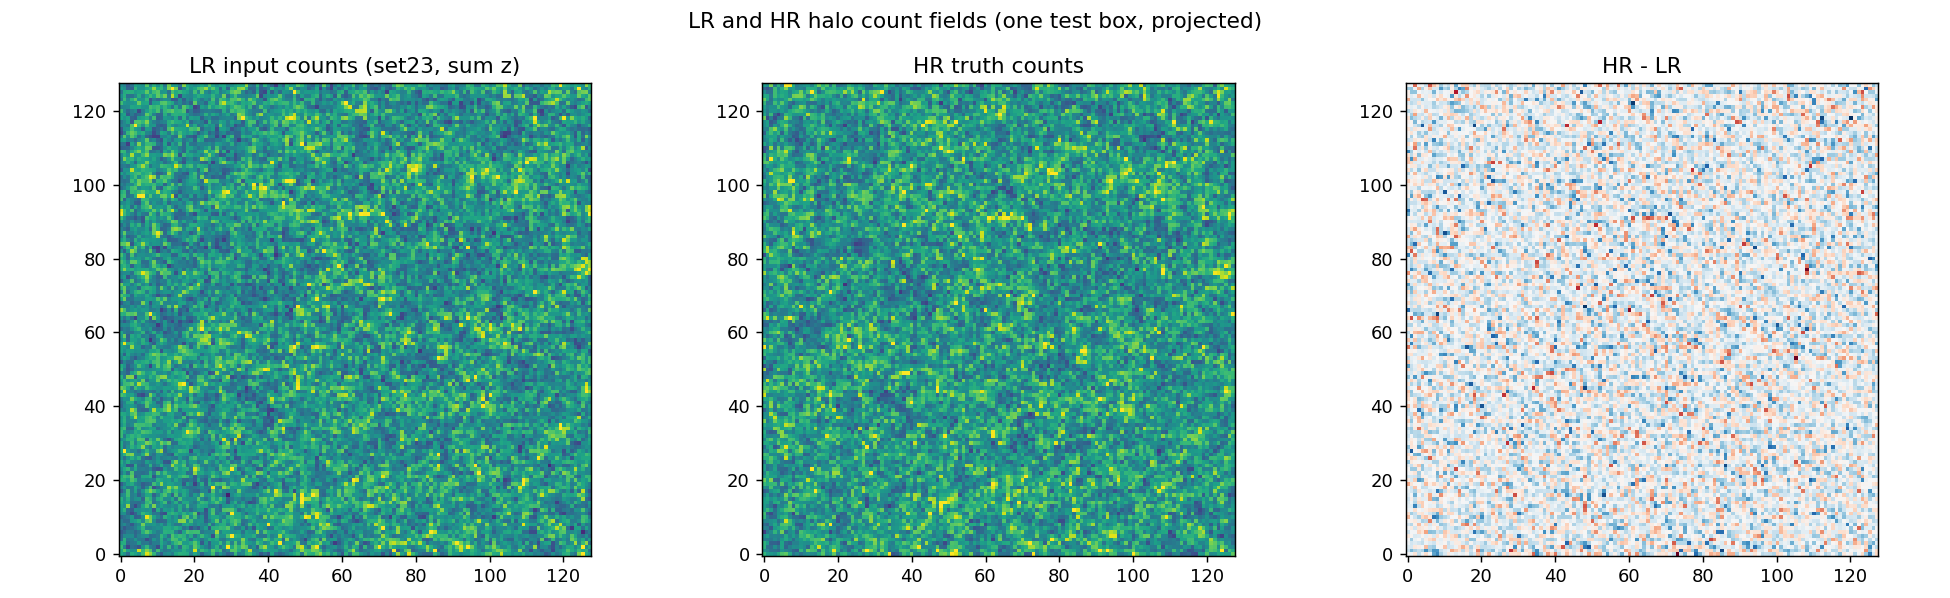
\includegraphics[width=0.9\linewidth]{figures_cmass/data_pair.png}
\caption{One LR/HR pair (projected count map). LR (FastPM, input) and HR
(Quijote N-body, target) share initial conditions and so share large-scale
structure, but differ cell-by-cell.}
\label{fig:srs-datapair}
\end{figure}

\paragraph{Model space (count transform).} The network does not learn on raw
counts; it learns in a compressed ``model space''. The default transform is
$\log(1+n)$, which tames the sparse heavy tail:
\begin{equation}
  y = \log(1+n), \qquad n = \exp(y)-1 \ \ (\text{clamped to } n\ge 0).
  \label{eq:srs-transform}
\end{equation}
Two alternative transforms exist in the code (\texttt{scale}: $n/\text{scale}$;
\texttt{delta}: model space is the overdensity itself), but all reported runs use
$\log(1+n)$. Power spectra are \emph{never} computed in model space; they are
always computed on the physical-count overdensity \SG{Is it okay if this is -1 when there are 0 halos?}
\begin{equation}
  \delta = \frac{n}{\bar n} - 1,
  \label{eq:srs-delta}
\end{equation}
with $\bar n$ the per-box mean count (the \texttt{perbox} setting used in all
runs).

\subsection{Data Pipeline (patching)}
\textit{Located in: \texttt{data/patch\_dataset\_cmass.py},
\texttt{data/patch\_dataset\_real.py} (shared patch ops).}

A model never sees the whole $128^3$ box at once. We cut the box into a
$2\times2\times2$ grid of $64^3$ \textbf{cores} (Table~\ref{tab:srs-notation}).
The cores tile the box exactly (stride $64$), so they reconstruct the box
bit-for-bit with no gaps and no double counting, the dataset's self-test
asserts this. Each model \emph{input} is a core grown by \texttt{pad} voxels on
every side, taken from the true neighbour cells with periodic wrap at the box
edge (\texttt{extract\_patch} uses \texttt{numpy.take(\dots, mode="wrap")}). So
with \texttt{pad}${=}8$ the input is $80^3$ and neighbouring patches overlap by
$2\cdot\texttt{pad}=16$ voxels; the HR \emph{target} is always the bare $64^3$
core. Because each simulation is one continuous periodic box that we crop
ourselves, the patches are real neighbours by construction, there is no data
seam (unlike the Lagrangian patches of \S5). \SG{Isn't the patch construction same in both?}

\begin{table}[t]
\centering
\caption{Notation for the CMASS count-field pipeline.}
\label{tab:srs-notation}
\begin{tabular}{llp{7.2cm}}
\toprule
Symbol & Value & Meaning \\
\midrule
$N_\text{full}$    & $128$ & full box side (voxels) \\
$P$ (\texttt{PATCH}) & $64$ & core side (voxels) \\
$N_\text{patches}$ & $8$ & cores per box ($2{\times}2{\times}2$) \\
\texttt{pad}       & $0$ (Arm A) / $8$ (Arm B) & halo width added to each face by periodic wrap \\
$L_\text{box}$     & $1000\ \mathrm{Mpc}/h$ & box side \\
$\mathbf s$        & $\in\mathbb R^5$ & cosmology vector $(\Omega_m,\Omega_b,h,n_s,\sigma_8)$ \\
$\bar n$           & per-box mean & mean count used to form $\delta=n/\bar n-1$ \\
\bottomrule
\end{tabular}
\end{table}

\begin{figure}[t]
\centering
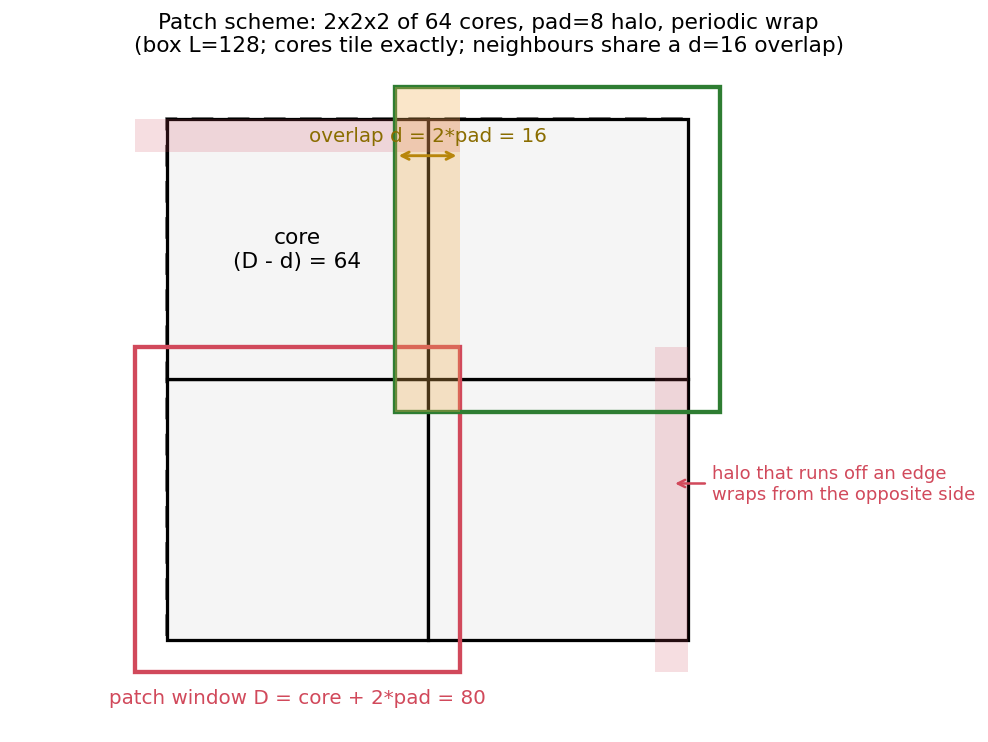
\includegraphics[width=0.82\linewidth]{figures_cmass/pipeline_patching.png}
\caption{Patch scheme. The box is cut into a $2{\times}2{\times}2$ grid of
$64^3$ cores that tile it exactly. With \texttt{pad}${>}0$ each patch is grown by
a halo of real neighbour cells (periodic wrap); only the central core is kept
and placed back.}
\label{fig:srs-patching}
\end{figure}

\paragraph{Per-simulation item.} Indexed by simulation, the dataset returns, for
all $8$ cores at once: the LR patches \texttt{lr\_in} of shape
$(8,\,1,\,64{+}2\,\texttt{pad},\,\cdot,\,\cdot)$ in model space, the HR cores
\texttt{hr\_tgt} of shape $(8,\,1,\,64,\,64,\,64)$, the style $\mathbf s$, and
the simulation index. The trainer flattens the $8$-core axis into the batch.

\begin{algorithm}[H]
\caption{\textsc{ExtractPatches} (one simulation)}
\label{alg:srs-extract}
\begin{algorithmic}[1]
\Require LR box $\mathbf L\in\mathbb R^{1\times128^3}$, HR box $\mathbf H$, \texttt{pad}
\State map $\mathbf L,\mathbf H$ to model space via Eq.~\ref{eq:srs-transform}
\For{$p=0,\dots,7$}
  \State $(i,j,k)\gets\textsc{unravel}(p,(2,2,2))$ \Comment{core origin $(64i,64j,64k)$}
  \State $\mathbf L_p\gets$ core $p$ grown by \texttt{pad} on each face, periodic wrap \Comment{$(64{+}2\,\texttt{pad})^3$}
  \State $\mathbf H_p\gets$ bare core $p$ \Comment{$64^3$}
\EndFor
\State \Return $\{(\mathbf L_p,\mathbf H_p)\}_{p=0}^{7}$, style $\mathbf s$
\end{algorithmic}
\end{algorithm}

\subsection{Model: Input/Output Specification}
\textit{Implementation: \texttt{map2map/models/styled\_srsgan.py}
(\texttt{G\_correct}, \texttt{D\_const}).}

\paragraph{What the generator computes.} The generator is a
\textbf{same-resolution residual} network: it does not change the grid size, and
it predicts a correction that is \emph{added} to the input. In model space,
\begin{equation}
  \mathrm{SR} \;=\; \mathrm{LR} \;+\; G(\mathrm{LR},\,\mathbf s,\,\mathbf z),
  \label{eq:srs-residual}
\end{equation}
where $\mathbf s$ is the cosmology vector and $\mathbf z$ is an injected noise
field (see below). Inputs and outputs are listed in
Table~\ref{tab:srs-model-io}; the generator is run once per core (the $8$ cores
of a box form a batch).

\begin{table}[t]
\centering
\caption{Tensors consumed/produced by the generator \texttt{G\_correct} for one
core (batch dimension omitted). Here $D=64{+}2\,\texttt{pad}$.}
\label{tab:srs-model-io}
\begin{tabular}{lll}
\toprule
Symbol & Shape & Meaning \\
\midrule
$\mathbf x$ (\texttt{x})       & $(1,D,D,D)$ & LR patch, model space (input) \\
$\mathbf s$ (\texttt{style})   & $(5,)$      & cosmology vector \\
$\mathbf z$ (\texttt{noise\_list}) & $2\cdot\texttt{num\_blocks}$ cubes $(1,D,D,D)$ & injected noise; fixed at inference, random in training \\
$G(\cdot)$                     & $(1,D,D,D)$ & predicted residual $\delta$ (added to $\mathbf x$) \\
\bottomrule
\end{tabular}
\end{table}

\paragraph{Internal composition.} $G$ is a constant-resolution StyleGAN2-style
network (no up/down-sampling), built from:
\begin{enumerate}
  \item \texttt{block0}: a $1{\times}1{\times}1$ style-modulated convolution
  (\texttt{ConvStyled3d}) lifting the $1$-channel input to $c_0$ channels,
  followed by a leaky ReLU.
  \item \texttt{num\_blocks} ($=4$) constant-resolution H-blocks
  (\texttt{HBlock\_const}). Each block, in order: inject noise $\to$
  $3{\times}3{\times}3$ \texttt{ConvStyled3d} (periodic ``circular'' padding)
  $\to$ leaky ReLU $\to$ inject noise $\to$ $3{\times}3{\times}3$
  \texttt{ConvStyled3d} $\to$ leaky ReLU $\to$ a $1{\times}1{\times}1$ projection
  to the output channel, accumulated into a running output $y$. The final return
  is $\mathbf x + y$ (Eq.~\ref{eq:srs-residual}).
\end{enumerate}
The channel widths come from \texttt{chan\_base} ($=128$) halved per block and
clamped to $[64,512]$. Two mechanisms make the convolutions depend on side
information:
\begin{itemize}
  \item \textbf{Style modulation.} \texttt{ConvStyled3d} is the StyleGAN2
  modulated/demodulated convolution: the cosmology vector $\mathbf s$ scales the
  convolution weights, so the same network behaves differently for different
  cosmologies. This is the only path by which $\mathbf s$ enters.
  \item \textbf{Noise injection.} Each \texttt{ConvStyled3d} is preceded by a
  per-channel learned-standard-deviation noise add (\texttt{\_NoiseInject}). At
  training time the noise is fresh Gaussian each call; at inference a
  \emph{fixed} list of noise cubes (seeded, built by \texttt{build\_noise\_list})
  is reused so outputs are reproducible. The noise is what lets the model produce
  a plausible small-scale field rather than a single blurred guess.
\end{itemize}

\paragraph{Discriminator.} \texttt{D\_const} is a constant-input-resolution
critic conditioned on the same style $\mathbf s$. It runs a head
\texttt{ConvStyled3d} then \texttt{num\_blocks} strided down-blocks (each a
periodic $3{\times}3{\times}3$ \texttt{ConvStyled3d} $+$ leaky ReLU $+$
$2{\times}$ average pool), a $1{\times}1{\times}1$ tail, and a final
$1{\times}1{\times}1$ projection to one channel, averaged over space to a single
logit per core.

\subsection{Training Step}
\textit{Located in: \texttt{train\_patch\_cmass.py}.}

The generator is trained per core (stitching is \emph{not} part of the
gradient). The total generator loss is a weighted sum of three terms,
\begin{equation}
  \mathcal L_G \;=\; \lambda_\text{adv}\,\mathcal L_\text{adv}
                  + \lambda_\text{rec}\,\mathcal L_\text{rec}
                  + \lambda_\text{pk}\,\mathcal L_\text{pk},
  \label{eq:srs-lossG}
\end{equation}
with (defaults from the original run script; see the protocol update below for
the values now in use):
\begin{itemize}
  \item \textbf{Reconstruction} $\mathcal L_\text{rec}=\lVert \mathrm{SR}-\mathrm{HR}\rVert_1$,
  a plain $L_1$ in model space (optionally Gaussian-smoothed; smoothing off in
  all runs).
  \item \textbf{Power-spectrum} $\mathcal L_\text{pk}$, the mean-squared error
  between the $\log_{10}$ power spectra of SR and HR, computed on the
  \emph{physical-count overdensity} of the $64^3$ core (Eqs.~\ref{eq:srs-transform}--\ref{eq:srs-delta}),
  Hann-windowed, with the HR side detached:
  \begin{equation}
    \mathcal L_\text{pk} = \frac{1}{|K|}\sum_{k\in K}
      \big(\log_{10} P_\text{SR}(k) - \log_{10} P_\text{HR}(k)\big)^2 .
    \label{eq:srs-pkloss}
  \end{equation}
  \item \textbf{Adversarial} $\mathcal L_\text{adv}=\mathrm{softplus}\!\big({-}D(\mathrm{SR},\mathbf s)\big)$,
  the non-saturating GAN generator loss.
\end{itemize}

\paragraph{Protocol update: what region the reconstruction and adversarial
terms see.} A \texttt{--pad-loss} setting controls how much of the generator's
output the $L_1$ and adversarial terms are computed on, independent of
\texttt{pad} itself:
\begin{itemize}
  \item \texttt{crop} (trim-aware, the setting used for Arm B above): the loss
  is computed only on \textsc{cropInterior}$(G(\mathbf x,\mathbf s),\,\texttt{pad})$,
  the $64^3$ core that is actually kept at inference time, against the bare
  $64^3$ HR core. The model is trained on exactly the region it will be graded
  on.
  \item \texttt{full}: the loss is computed on the whole $(64{+}2\,\texttt{pad})^3$
  output, against a correspondingly padded HR target (the dataset's
  \texttt{pad\_target} option). The model is trained as if the halo region it
  will later be trimmed off also mattered.
\end{itemize}
Concretely, let $\texttt{loss\_crop}=\texttt{pad}$ under \texttt{crop} and $0$
under \texttt{full}; every place above that writes $\mathrm{SR}$ means
$\textsc{cropInterior}(G(\mathbf x,\mathbf s),\,\texttt{loss\_crop})$, and the
Hann window and $P(k)$ estimator in $\mathcal L_\text{pk}$ are sized to match.
This is a controlled test of two ways padding could fail to help: see the
protocol-update subsection below for the result.

The discriminator is trained with the non-saturating GAN loss plus a lazy $R_1$
gradient penalty applied every \texttt{r1\_every} steps:
\begin{equation}
  \mathcal L_D = \mathrm{softplus}\!\big({-}D(\mathrm{HR})\big)
               + \mathrm{softplus}\!\big(D(\mathrm{SR})\big)
               + \tfrac{1}{2}\lambda_{R_1}\,\mathbb E\big\lVert \nabla_{\!x} D(x,\mathbf s)\big\rVert^2 .
  \label{eq:srs-lossD}
\end{equation}

\begin{algorithm}[H]
\caption{CMASS patch-GAN training step (one batch of cores)}
\label{alg:srs-train}
\begin{algorithmic}[1]
\Require LR patches $\mathbf x$, HR targets $\mathbf h$ (padded iff \texttt{pad-loss=full}),
         style $\mathbf s$, \texttt{pad}, \texttt{loss\_crop} ($=\texttt{pad}$ if \texttt{crop} else $0$),
         weights $\lambda_\text{adv},\lambda_\text{rec},\lambda_\text{pk},\lambda_{R_1}$
\Statex \textbf{// Discriminator}
\State $\hat{\mathbf h}\gets \textsc{cropInterior}\big(G(\mathbf x,\mathbf s),\,\texttt{loss\_crop}\big)$ \Comment{no grad}
\State $\mathcal L_D \gets \mathrm{softplus}({-}D(\mathbf h,\mathbf s)) + \mathrm{softplus}(D(\hat{\mathbf h},\mathbf s))$
\If{step $\bmod\ \texttt{r1\_every} = 0$} $\mathcal L_D \mathrel{+}= \tfrac12\lambda_{R_1}\texttt{r1\_every}\cdot R_1(D,\mathbf h,\mathbf s)$ \EndIf
\State update $D$ (Adam, grad-clip)
\Statex \textbf{// Generator}
\State $\hat{\mathbf h}\gets \textsc{cropInterior}\big(G(\mathbf x,\mathbf s),\,\texttt{loss\_crop}\big)$
\State $\mathcal L_\text{adv}\gets \mathrm{softplus}({-}D(\hat{\mathbf h},\mathbf s))$
\State $\mathcal L_\text{rec}\gets \lVert \hat{\mathbf h}-\mathbf h\rVert_1$
\State $\mathcal L_\text{pk}\gets$ Eq.~\ref{eq:srs-pkloss} on Hann-windowed overdensity of $\hat{\mathbf h}$, $\mathbf h$
       (skip if $\lambda_\text{pk}{=}0$)
\State $\mathcal L_G \gets \lambda_\text{adv}\mathcal L_\text{adv}+\lambda_\text{rec}\mathcal L_\text{rec}+\lambda_\text{pk}\mathcal L_\text{pk}$
\State update $G$ (Adam, grad-clip)
\end{algorithmic}
\end{algorithm}

\paragraph{Validation and checkpoint selection.} After each epoch we stitch the
full $128^3$ SR box for up to $40$ validation sims and report the stitched
$L_1$/voxel and the stitched-$128$ power-spectrum RMS against HR
(\S\ref{sec:srs-eval}, Eq.~\ref{eq:srs-pkrms}). A \texttt{--select} setting
chooses which of the two the saved \texttt{best.pt} tracks: \texttt{pk} (the
original setting, lowest stitched validation Pk RMS) or \texttt{l1} (lowest
stitched validation $L_1$/voxel). Selection is always on the stitched full box,
not the per-core training loss. Runs that also train with $\lambda_\text{pk}{=}0$
use \texttt{--select l1}, since selecting on Pk RMS while not training on it
would reintroduce the same metric leak in a different place.

\subsection{Inference}
\textit{Located in: \texttt{infer\_stitch\_cmass.py}.}

For one simulation: load the LR $128^3$ count box, map it to model space, run $G$
on each of the $8$ cores (with the periodic-wrap halo in Arm B), crop the halo,
stitch the cores into a $128^3$ model-space box, invert the transform to physical
counts, and clamp. \SG{are all outputs later mapped to integers, or are we fine with non-integer number of halos?} The injected noise list is fixed (seeded) so the output is
reproducible.

\begin{algorithm}[H]
\caption{CMASS inference + stitch (one simulation)}
\label{alg:srs-infer}
\begin{algorithmic}[1]
\Require LR box $\mathbf L$, style $\mathbf s$, trained $G$, mode (naive/overlap), fixed noise $\mathbf z$
\State $\texttt{pad}\gets 0$ if naive else value from checkpoint ($8$)
\State map $\mathbf L$ to model space (Eq.~\ref{eq:srs-transform})
\For{$p=0,\dots,7$}
  \State $\mathbf x_p\gets$ patch $p$ (core grown by \texttt{pad}, periodic wrap)
  \State $\mathbf c_p\gets \textsc{cropInterior}\big(G(\mathbf x_p,\mathbf s,\mathbf z),\,\texttt{pad}\big)$ \Comment{$64^3$ core, model space}
\EndFor
\State $\mathbf S\gets \textsc{stitch}(\{\mathbf c_p\})$ \Comment{$128^3$, model space}
\State $\mathbf S\gets \exp(\mathbf S)-1$, clamp to $[0,\,C_\text{max}{=}200]$, replace NaN/Inf \Comment{physical counts}
\State \Return $\mathbf S$
\end{algorithmic}
\end{algorithm}

\subsection{Crop Stitching}

Stitching is \textbf{direct placement with no averaging}. Adjacent cores tile the
box exactly (stride $64$, no overlap between cores once the halo is dropped), so
each core's $64^3$ output is written straight into its slot. In Arm B the $80^3$
patch is corrected and only its central $64^3$ core is kept; the overlap halo is
context for the convolution, never written to the output.

\begin{algorithm}[H]
\caption{\textsc{Stitch} ($8$ cores $\to$ $128^3$)}
\label{alg:srs-stitch}
\begin{algorithmic}[1]
\Require cores $\{\mathbf c_p\}_{p=0}^{7}$, each $1\times64^3$
\State $\mathbf S\gets \mathbf 0\in\mathbb R^{1\times128^3}$
\For{$p=0,\dots,7$}
  \State $(i,j,k)\gets\textsc{unravel}(p,(2,2,2))$
  \State $\mathbf S[:,\,64i{:}64i{+}64,\,64j{:}\cdots,\,64k{:}\cdots]\gets \mathbf c_p$ \Comment{direct assignment}
\EndFor
\State \Return $\mathbf S$
\end{algorithmic}
\end{algorithm}

\subsection{Evaluation}
\label{sec:srs-eval}
\textit{Located in: \texttt{analysis/eval\_seam\_cmass.py},
\texttt{analysis/diag\_cmass.py}, \texttt{analysis/match\_stats\_cmass.py},
\texttt{analysis/power\_spectrum.py}, \texttt{inference/nde.py},
\texttt{evaluate.py}.}

We evaluate the SR field against HR at three levels: a seam check (does stitching
leave a join?), field statistics (does SR have the right structure?), and
cosmology (does SR give the same parameter posterior as HR?).

\paragraph{Power-spectrum summaries.} On the count overdensity (Eq.~\ref{eq:srs-delta})
we report the power spectrum $P(k)$, the transfer ratio, and the cross-coherence:
\begin{equation}
  T(k) = \frac{P_\text{SR}(k)}{P_\text{HR}(k)},
  \qquad
  r(k) = \frac{P_{\text{SR},\text{HR}}(k)}{\sqrt{P_\text{SR}(k)\,P_\text{HR}(k)}} .
  \label{eq:srs-Tr}
\end{equation}
$T(k)=1$ means SR has the right \emph{amount} of power at scale $k$ (amplitude);
$r(k)=1$ means SR has the structure in the right \emph{place} (phase). The
scalar power-spectrum error used for checkpoint selection and seam reporting is
the log-RMS over the resolved $k$-bins:
\begin{equation}
  \mathrm{PkRMS}_{\log_{10}} = \sqrt{\frac{1}{|K|}\sum_{k\in K}
    \big(\log_{10} P_\text{SR}(k) - \log_{10} P_\text{HR}(k)\big)^2 } .
  \label{eq:srs-pkrms}
\end{equation}

\paragraph{Seam diagnostic.} \texttt{eval\_seam\_cmass.py} bins the per-cell
count error $|{\mathrm{SR}-\mathrm{HR}}|$ by distance to the nearest core face
and forms a per-position error profile along each axis. The headline number is
the \textbf{$x{=}64$ internal-seam excess}: the error on the internal core
boundary plane divided by the interior error. A value near $1$ means stitching
leaves no seam. The box edge $x{=}0$ is a periodic-boundary control.

\paragraph{Field-match statistics.} \texttt{match\_stats\_cmass.py} reports, over
$16$ test boxes: the total-count ratio $\sum\mathrm{SR}/\sum\mathrm{HR}$, the
void fraction (cells $<0.5$), the real-space cell standard-deviation ratio
$\mathrm{std}(\mathrm{SR})/\mathrm{std}(\mathrm{HR})$ (a blur check), and the
cross-coherence $r(k)$ at large ($k<0.05$) and small ($k>0.2$) scales.

\paragraph{Cosmology (posterior consistency).} This is the strongest ``does SR
match HR'' test. We voxel-count $\to$ overdensity $\to$ $P(k)$ for every box, then
train a neural density estimator $q(\theta\mid P(k))$ on the training split using
\texttt{sbi} (\texttt{SNPE\_C} with a neural-spline-flow density estimator,
\texttt{inference/nde.py}); the summary is $\log_{10}P(k)$. We train one estimator
on HR ($q_\text{HR}$) and one on each SR arm ($q_\text{SR}$). For each test box we
draw $2000$ posterior samples from each, fit a Gaussian per parameter, and report
the per-parameter Gaussian KL (\texttt{evaluate.py}):
\begin{equation}
  \mathrm{KL}\big(\mathcal N(\mu_\text{HR},\sigma_\text{HR})\,\Vert\,\mathcal N(\mu_\text{SR},\sigma_\text{SR})\big)
  = \tfrac12\!\left[\log\frac{\sigma_\text{SR}^2}{\sigma_\text{HR}^2}
    + \frac{\sigma_\text{HR}^2+(\mu_\text{HR}-\mu_\text{SR})^2}{\sigma_\text{SR}^2} - 1\right].
  \label{eq:srs-kl}
\end{equation}
$\mathrm{KL}=0$ means SR gives the identical cosmology posterior to HR. The raw LR
field (no model), pushed through the same pipeline, is the control SR must beat.

We report this comparison in two forms, and it matters which is which:
\begin{itemize}
  \item \textbf{Cross-fidelity (primary).} $q_\text{SR}$ is trained on SR power
  spectra but \emph{evaluated on the HR} $P(k)$ of each test simulation, and
  compared to $q_\text{HR}$ evaluated on the same HR $P(k)$. This is the
  deployment scenario the project targets: HR simulations are too expensive to
  train an inference model on, so the inference model is trained on cheap SR
  output and must still work when applied to (HR-like) reality. The comparison
  against an LR-trained estimator on the same HR data measures whether sampling
  in HR space (SR) survives the distribution shift better than staying in LR
  space. This metric never appears in the training loss.
  \item \textbf{Own-data (secondary).} $q_\text{SR}$ trained and evaluated on SR
  vs $q_\text{HR}$ trained and evaluated on HR, each pipeline end-to-end on
  its own field type.
\end{itemize}

\subsection{Best-Run Configuration}
\textit{Run script: \texttt{scripts/train\_patch\_cmass.slurm}; checkpoints
\texttt{checkpoints/patch\_cmass\_\{A,B\}/best.pt}.}

Both arms use the identical configuration below; they differ only in \texttt{pad}
($0$ for Arm~A, $8$ for Arm~B). This is the configuration behind every number
in \S\ref{sec:srs-results}--\S\ref{sec:srs-next}.

\begin{lstlisting}[language=bash]
--transform log1p   --nbar perbox        # log(1+n) model space; per-box nbar
--epochs 30         --sims-per-batch 1    # patch-batch = 8 cores per step
--chan-base-g 128   --chan-base-d 64  --num-blocks 4
--lambda-adv 1.0    --lambda-rec 2.0  --lambda-pk 2.0   # generator weights
--lambda-r1 10.0    --r1-every 16                       # lazy R1
--lr-g 1e-4 --lr-d 1e-4  --beta1 0.0 --beta2 0.99       # Adam
--grad-clip 1.0     --val-max-sims 40    --select pk    # select on Pk RMS
\end{lstlisting}

The best checkpoint per arm is the one with the lowest stitched validation Pk RMS
(Eq.~\ref{eq:srs-pkrms}):

\begin{center}
\begin{tabular}{lc}
\toprule
arm & best stitched val PkRMS$_{\log_{10}}$ \\
\midrule
Arm A, naive (pad $0$)  & $0.0947$ \\
Arm B, overlap (pad $8$) & $0.0963$ \\
\bottomrule
\end{tabular}
\end{center}

\paragraph{Protocol update.} Following the mentor meeting reported in
\S\ref{sec:srs-followup}, the configuration above is no longer the one we train
with. Three settings changed:
\begin{lstlisting}[language=bash]
--lambda-pk 0.0      # power-spectrum term OFF (it was also our main metric)
--pad-loss crop|full # trim-aware vs trim-unaware padding, see below
--select l1          # select on stitched L1, not the term we removed
\end{lstlisting}
All results in \S\ref{sec:srs-followup} use this configuration. Runs under the
original configuration above (Arm A, Arm B, and everything derived from them in
\S\ref{sec:srs-results}--\S\ref{sec:srs-next}) remain valid as a record of that
protocol; they are superseded, not invalidated, by the update.

\subsection{Results: Does SR Match HR?}
\label{sec:srs-results}

All numbers are on the $200$-box test split unless noted.

\paragraph{1. Power spectrum (statistics).} Across the test set the SR power
spectrum tracks HR at every scale, and Arm A beats the no-model LR control on the
overall log-RMS (Fig.~\ref{fig:srs-srvshr}, computed by
\texttt{analysis/plot\_sr\_vs\_hr.py}).

\begin{table}[h]
\centering
\caption{SR vs HR power-spectrum agreement, $200$ test boxes. Transfer
$T(k)=P_X/P_\text{HR}$ (Eq.~\ref{eq:srs-Tr}); $1.0$ is perfect.}
\label{tab:srs-pk}
\begin{tabular}{lccc}
\toprule
field (vs HR) & PkRMS$_{\log_{10}}$ & $T$ at large scales ($k{<}0.1$) & $T$ at small scales ($k{>}0.3$) \\
\midrule
SR (Arm A, naive)    & $\mathbf{0.0607}$ & $0.95$ & $1.04$ \\
SR (Arm B, overlap)  & $0.0645$ & $0.93$ & $0.88$ \\
LR (no model, control) & $0.0641$ & $1.01$ & $1.01$ \\
\bottomrule
\end{tabular}
\end{table}

\begin{figure}[t]
\centering
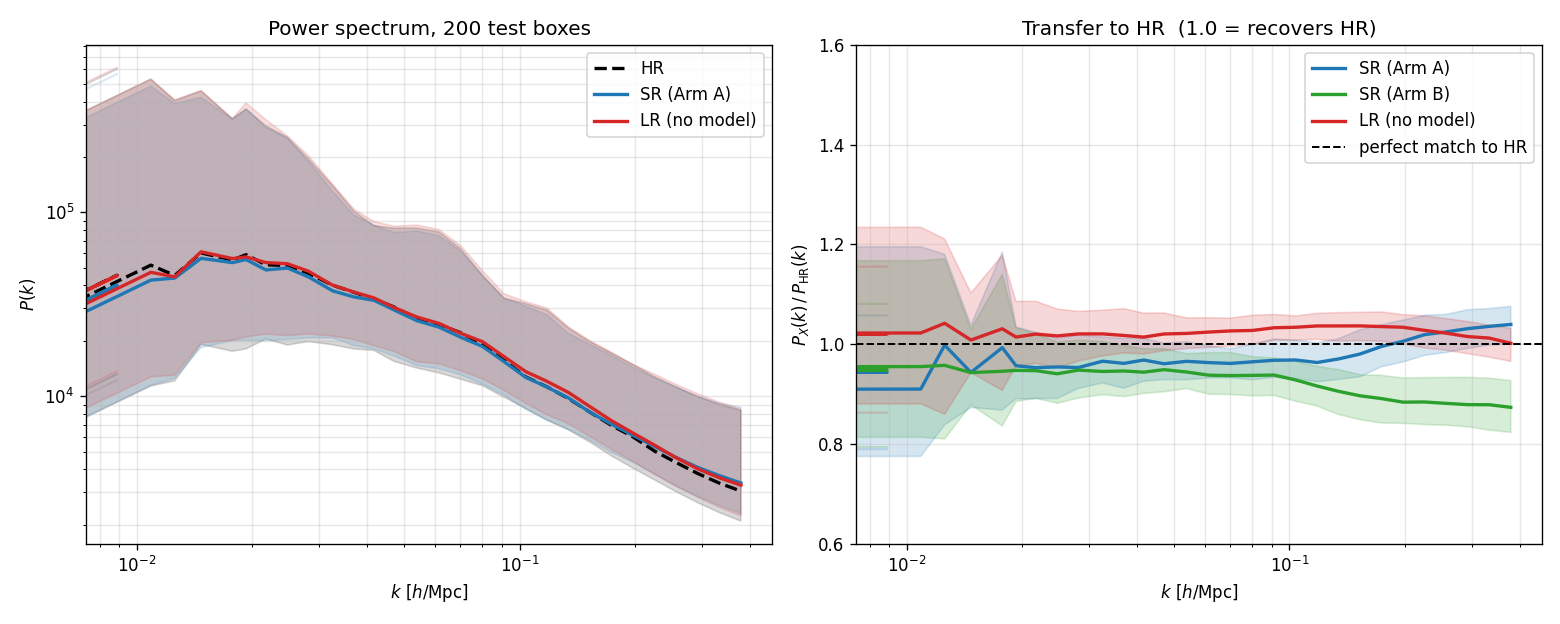
\includegraphics[width=0.98\linewidth]{figures_cmass/sr_vs_hr_pk.png}
\caption{\textbf{Left:} $P(k)$ of HR, SR (Arm A), and LR over $200$ test boxes
(median $+$ $16/84\%$ band). \textbf{Right:} transfer to HR; $1.0$ recovers HR.
SR (Arm A) sits near $1$ at all scales; Arm B's overlap blending slightly
suppresses small-scale power (transfer $0.88$).}
\label{fig:srs-srvshr}
\end{figure}

\paragraph{2. Field structure.} Beyond the power spectrum, SR keeps the field
structure of HR (Arm A, $16$ test boxes, \texttt{match\_stats\_cmassA.txt}):

\begin{table}[h]
\centering
\caption{SR vs HR field-match statistics (Arm A).}
\label{tab:srs-match}
\begin{tabular}{lll}
\toprule
quantity & value & reading \\
\midrule
total count ratio $\sum\mathrm{SR}/\sum\mathrm{HR}$ & $0.965\pm0.172$ & counts conserved on average; large per-box scatter \\
real-space std ratio & $1.008\pm0.100$ & clustering amplitude matches; not blurred \\
void fraction SR / HR ($<0.5$) & $0.855$ / $0.833$ & SR keeps voids empty, like HR \\
cross-coherence $r$, $k<0.05$ & $0.951$ & large-scale structure matches cell-by-cell \\
cross-coherence $r$, $k>0.2$ & $0.403$ & small-scale structure decorrelates \\
\bottomrule
\end{tabular}
\end{table}

\paragraph{3. Cosmology.} The cosmology comparison in the original report used
mislabeled cosmologies, an indexing bug we describe and fix in
\S\ref{sec:srs-correction}, so those numbers are not shown here. With correct
labels a single box constrains $\Omega_m$ and $\sigma_8$; at the power spectrum
level the raw LR field is already HR-like, while at the field level an SR-trained
posterior transfers to HR and an LR-trained one does not
(\S\ref{sec:srs-correction}, Table~\ref{tab:srs-corrected}).

\paragraph{4. Seam.} Neither arm introduces a stitching seam: the $x{=}64$
internal-seam excess is $\approx1$ for both
(Table~\ref{tab:srs-seam}, Fig.~\ref{fig:srs-seam}). Arm A shows a mild generic
ripple near \emph{any} boundary plane (seam-distance ratio $1.17$); Arm B's
overlap removes it ($1.00$) at a small cost in Pk RMS.

\begin{table}[h]
\centering
\caption{Seam and stitched-fidelity metrics, $200$ test boxes. ``Excess'' is
boundary error over interior error; $\approx1$ means no seam.}
\label{tab:srs-seam}
\begin{tabular}{lccp{5.2cm}}
\toprule
metric & Arm A naive & Arm B overlap & reading \\
\midrule
$x{=}64$ internal-seam excess & $0.9934$ & $0.9998$ & no internal seam either arm \\
seam-distance ratio ($d{=}0/d{\ge}8$) & $1.1729$ & $1.0032$ & generic boundary ripple, removed by overlap \\
$x{=}0$ periodic edge (control) & $0.9930$ & $0.9993$ & box edge behaves like interior \\
stitched PkRMS$_{\log_{10}}$ vs HR & $0.0637$ & $0.0678$ & stitched power-spectrum match \\
\bottomrule
\end{tabular}
\end{table}

\begin{figure}[t]
\centering
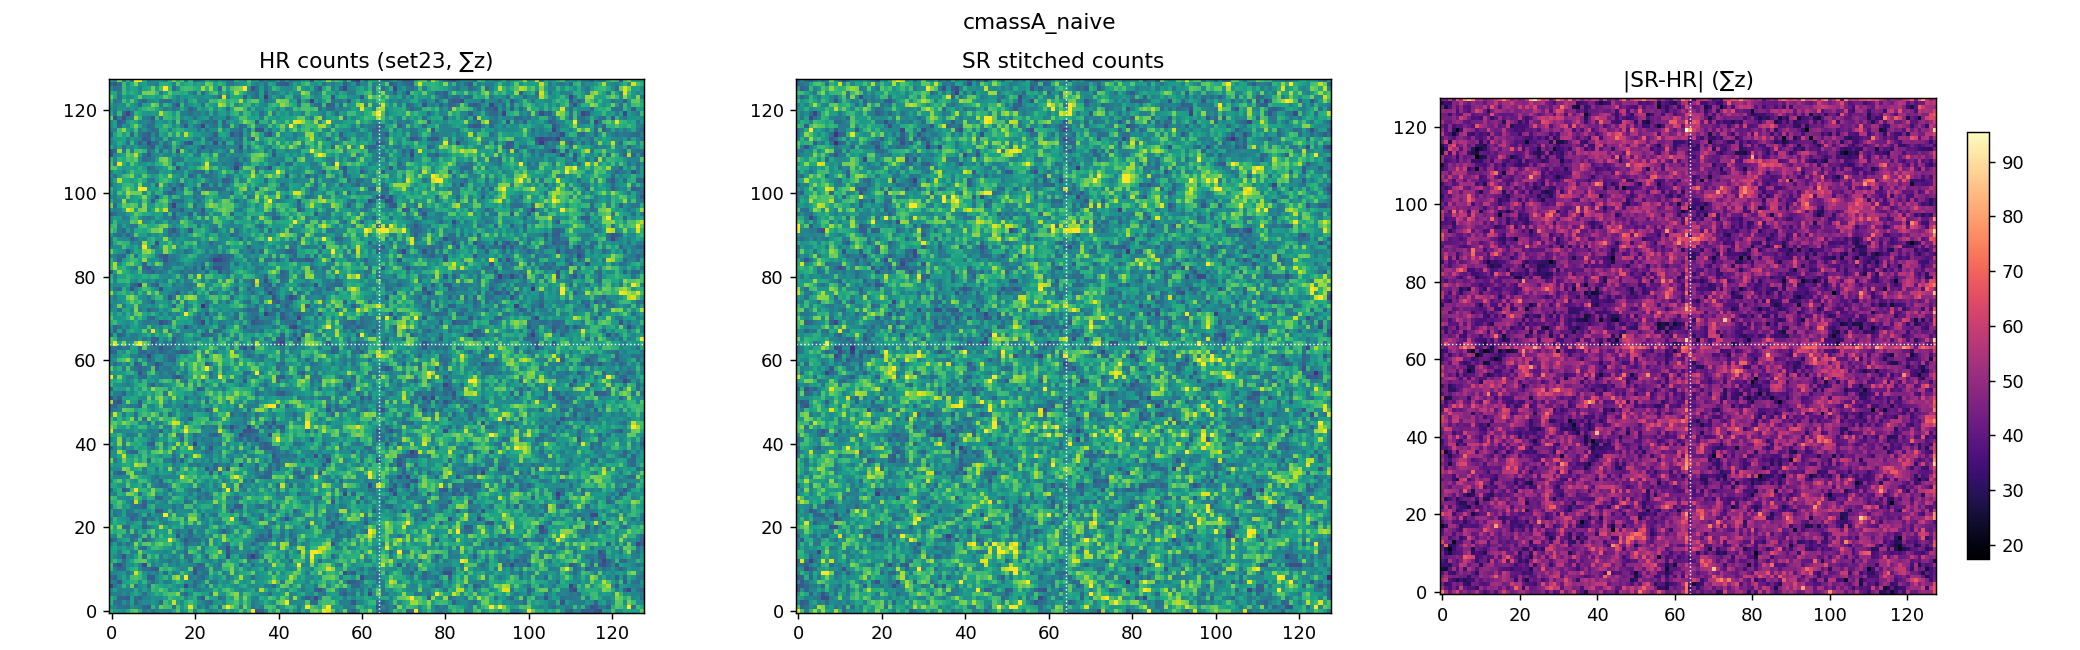
\includegraphics[width=0.95\linewidth]{figures_cmass/seam_cmassA_naive_slice.png}
\caption{Projected count maps for one test box (Arm A): HR, stitched SR, and the
absolute residual $|\mathrm{SR}-\mathrm{HR}|$. White dotted lines mark the
$x{=}64$, $y{=}64$ core boundaries; the residual shows no elevated ridge along
them.}
\label{fig:srs-seam}
\end{figure}

\paragraph{Per-scale diagnostic panels.} Figure~\ref{fig:srs-pkpanel} shows the
full-box $P(k)$, transfer, and cross-coherence for Arm A. The transfer sits near
$1$ at all scales (right amount of power); the cross-coherence is near $1$ at
large scales and falls toward small scales (structure placement is recovered at
large scales only). The per-patch panel
(\texttt{figures\_cmass/pk\_panel\_patch\_cmassAfix.png}) and the projection panels
(\texttt{projection\_box\_cmassAfix\_set23.png},
\texttt{projection\_patch\_cmassAfix\_set23\_p0.png}) tell the same story; Arm~B's
panels carry the \texttt{cmassB} suffix.

\begin{figure}[t]
\centering
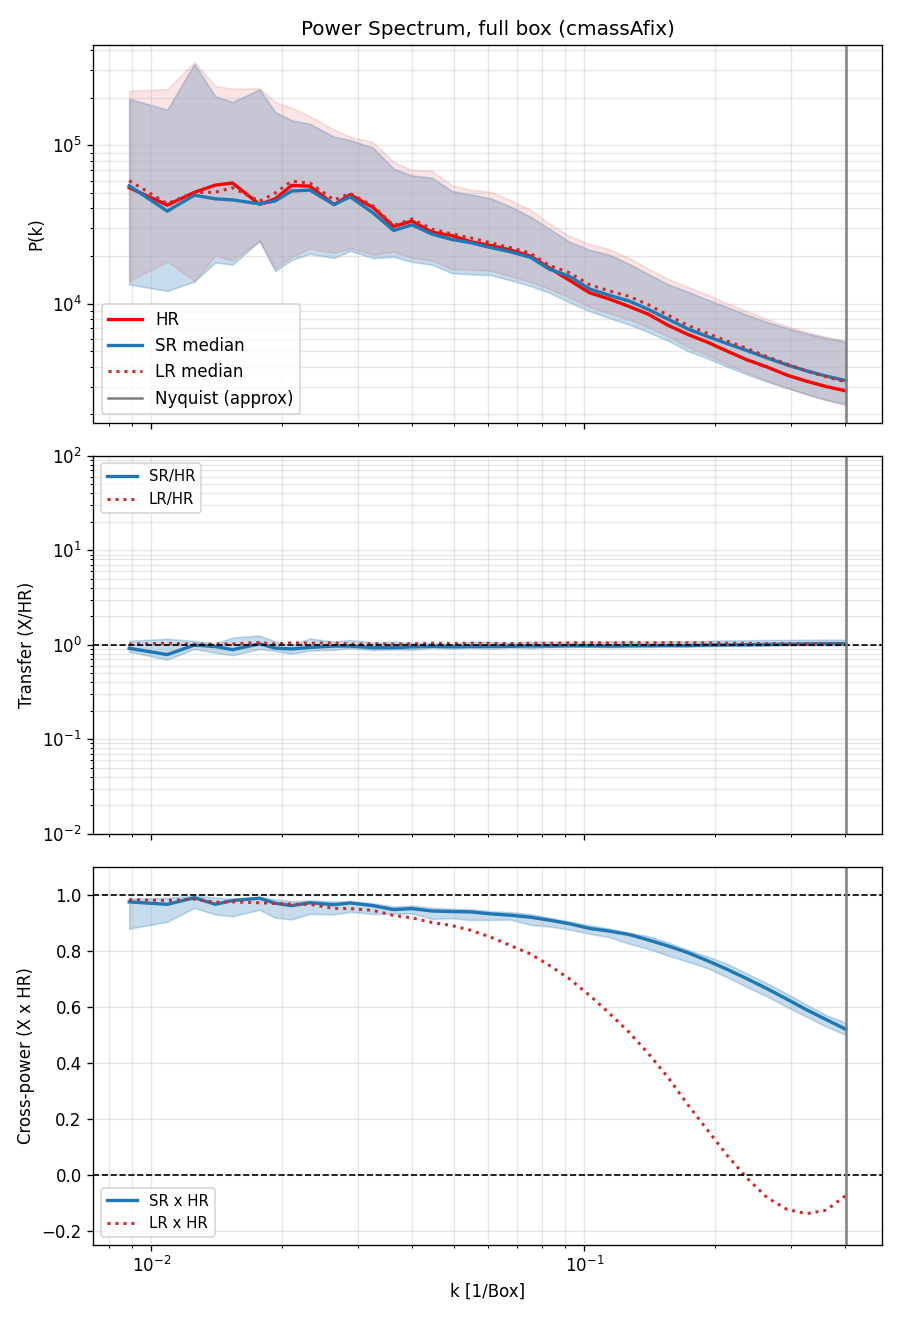
\includegraphics[width=0.5\linewidth]{figures_cmass/pk_panel_box_cmassAfix.png}
\caption{Full-box diagnostic for the conditioned generator (fiducial cosmology,
$16$ test boxes): $P(k)$ of HR (red), SR (blue median $+$ band), and LR (dotted
red); transfer $T(k)=P_X/P_\text{HR}$ on a linear axis with the 16 to 84
percentile band for both SR and LR, the legend reporting the RMS deviation of
each ratio from unity; and cross-coherence $r(k)$. The SR median transfer sits
below unity for $k<0.1$, a systematic large-scale power deficit of roughly 5 to
10 percent, while LR sits slightly above unity; SR does not tighten the transfer
scatter relative to LR. In $r(k)$, SR stays near unity to smaller scales while
LR decorrelates.}
\label{fig:srs-pkpanel}
\end{figure}

\subsection{Diagnostic: What is NOT Working}

\paragraph{Small-scale structure decorrelates, and this is fundamental.} SR
matches HR cell-by-cell at large scales ($r{=}0.95$ for $k<0.05$) but loses the
match at small scales ($r{=}0.40$ for $k>0.2$, Table~\ref{tab:srs-match}). This
is not a capacity bug: it is set by how much information the LR input carries
about HR. LR and HR share large-scale modes but the voxel-by-voxel LR$\leftrightarrow$HR
correlation is only $\approx0.06$, so the exact small-scale realization is simply
not present in the input. The model can match the small-scale \emph{statistics}
(transfer $\approx1$, real-space std ratio $1.008$) but cannot reproduce the
exact placement of individual halos. The noise injection
(Eq.~\ref{eq:srs-residual}) exists precisely because of this: it draws a
plausible small-scale field rather than regressing to a blur.

\paragraph{Per-box total-count scatter.} The total halo count is conserved on
average but with $\sim17\%$ per-box scatter ($\sum\mathrm{SR}/\sum\mathrm{HR}=
0.965\pm0.172$). A count-aware output head (predict a rate and sample Poisson
counts) would tighten this; it is the one clearly addressable imperfection. \SG{I would think this isn't necessary to fix, we don't care about the number of halos after all.}

\paragraph{Overlap suppresses small-scale power.} Arm B's overlap blending lowers
the small-scale transfer to $0.88$ (Table~\ref{tab:srs-pk}), so on the power
spectrum the naive Arm A is the better super-resolver. Overlap removes a small
generic boundary ripple but buys no fidelity, because on this continuous count
data there is no real seam to fix, the clean version of the mentor 2.1 vs 2.2
comparison.

\paragraph{Where the cosmology value is.} At the power spectrum level the raw LR
field is already close to HR, since they share large-scale modes, so the power
spectrum is a forgiving summary with little headroom. The model's value is at the
field level (variance, voids, small-scale structure), which the power spectrum
summary is insensitive to. The corrected cross-fidelity in
\S\ref{sec:srs-correction} bears this out: SR and LR are indistinguishable at the
power spectrum level, but at the field level an SR-trained posterior transfers to
HR while an LR-trained one does not.

\subsection{What I'm Trying Next}
\label{sec:srs-next}

The diagnostics above point to one limit that may be fundamental (small-scale
decorrelation) and a few that are clearly fixable (count scatter, small-scale
realism). The plan below is ordered so that we \emph{measure} the limit before
spending effort trying to beat it. None of these results are in yet; this is the
roadmap, not an experiment log.

\paragraph{Step 0, measure the information ceiling first.} Before trying to
improve the small-scale match, we need to know whether $r{=}0.40$ at small scales
(Table~\ref{tab:srs-match}) is the best any model could do from this input, or a
weakness of the current one. Two cheap diagnostics settle it:
\begin{itemize}
  \item \textbf{LR$\leftrightarrow$HR cross-coherence $r_\text{LR,HR}(k)$.} The
  cross-coherence of the \emph{raw input} against HR (no model) is the ceiling:
  no function of LR can place small-scale structure better than the input
  already correlates with HR. If $r_\text{SR,HR}(k)\approx r_\text{LR,HR}(k)$ at
  small $k$, the model is already at the ceiling and the limit is fundamental;
  if it sits well below, there is recoverable structure left on the table. (Only
  per-box $P(k)$ is currently saved, not the cross-spectrum, so this needs one
  re-run that keeps the fields.)
  \item \textbf{No-noise ablation.} Train the same generator with the noise
  injection off (a plain regressor). Theory predicts this should \emph{raise} the
  small-scale cross-coherence a little (a regressor targets the conditional mean,
  the best cell-by-cell predictor) but \emph{lower} the small-scale transfer well
  below $1$ (the conditional mean is blurry). Seeing exactly that trade-off would
  confirm that the noise/GAN is the right choice for a power-spectrum target, and
  would quantify how much cell-by-cell accuracy is being traded for correct
  statistics.
\end{itemize}

\paragraph{Step 1, fix the count scatter and small-scale realism (independent
of the ceiling).} These help regardless of what Step 0 finds:
\begin{itemize}
  \item \textbf{Count-aware (Poisson) output head.} Instead of predicting a
  count directly, predict a non-negative rate $\lambda$ per cell and sample the
  count as $n\sim\mathrm{Poisson}(\lambda)$. Halo counts are discrete and sparse,
  so a Poisson head models the small-scale graininess as actual shot noise rather
  than a smeared residual, and should tighten the $\sim17\%$ per-box total-count
  scatter (Table~\ref{tab:srs-match}), the one clearly addressable imperfection.
  \item \textbf{Explicit statistics terms in the loss.} Add a one-point PDF /
  variance matching term so small-scale sharpness is enforced directly, rather
  than relying on the adversarial term alone to find it.
  \item \textbf{Loss rebalance.} The current weights are $\lambda_\text{rec}{=}2$,
  $\lambda_\text{pk}{=}2$, $\lambda_\text{adv}{=}1$
  (Eq.~\ref{eq:srs-lossG}). The $L_1$ term blurs; lowering it and raising the
  adversarial weight should push toward correct statistics, at a known cost in
  cell-by-cell accuracy, per the same trade-off as the no-noise ablation.
\end{itemize}

\paragraph{Step 2, extract more of the available information (only if Step 0
shows headroom).} If $r_\text{SR,HR}$ sits below the LR$\leftrightarrow$HR
ceiling, the model is under-using its input. A larger receptive field, or feeding
each patch more neighbour context, would let it use more of the LR field to
predict the residual. This only helps if there is headroom to recover.

\paragraph{Step 3, raise the ceiling by changing the \emph{input}, not the
model.} The small-scale cell-by-cell limit is set by the information in the LR
input (the voxel-by-voxel LR$\leftrightarrow$HR correlation is only
$\approx0.06$). No amount of model capacity raises that; only more informative
inputs do. Candidates: feed the shared small-scale \emph{initial conditions}
(which the coarse LR count field has discarded), or add the LR velocity / particle
fields. This is the only route to a meaningful gain in small-scale cross-coherence,
and is the natural bridge to the displacement-field model of \S5, which already
carries that extra information.

\paragraph{Summary.} Steps 0--1 are the near-term plan: measure the ceiling, then
add a Poisson head and statistics losses to fix the count scatter and sharpen the
small-scale field. Steps 2--3 are contingent on what Step 0 reveals. For a
cosmology deliverable the priority is statistical fidelity (which Steps 0--1
target); exact small-scale reconstruction (Step 3) is a larger, input-level
change worth it only if cell-by-cell recovery becomes the goal.

\subsection{Follow-Up Results: New Protocol from the Mentor Meeting}
\label{sec:srs-followup}

A mentor meeting after the report above changed two things about how we train
and evaluate this model. First, the real goal is not to match HR with SR by
itself. The real goal is to train a posterior model on SR output and have it
work well when it is tested on real HR data, since HR simulations are too
expensive to train a posterior model on directly. Second, the power spectrum
term was removed from the training loss, since it was also our main success
metric and that is a weak test. This subsection reports what we found. Some of
the training runs below are still in progress at the time of writing, so
numbers marked as current are read from the latest completed epoch, not a
final result.

\paragraph{Held-out check: the bispectrum.} A fair worry is that our power
spectrum result looks good only because the power spectrum was also in the
training loss. To check this we measured the bispectrum, a higher-order
statistic that was never used anywhere in training or model selection. If SR
only matches the power spectrum and nothing else, the bispectrum should show
no improvement over the raw LR input.

\begin{figure}[t]
\centering
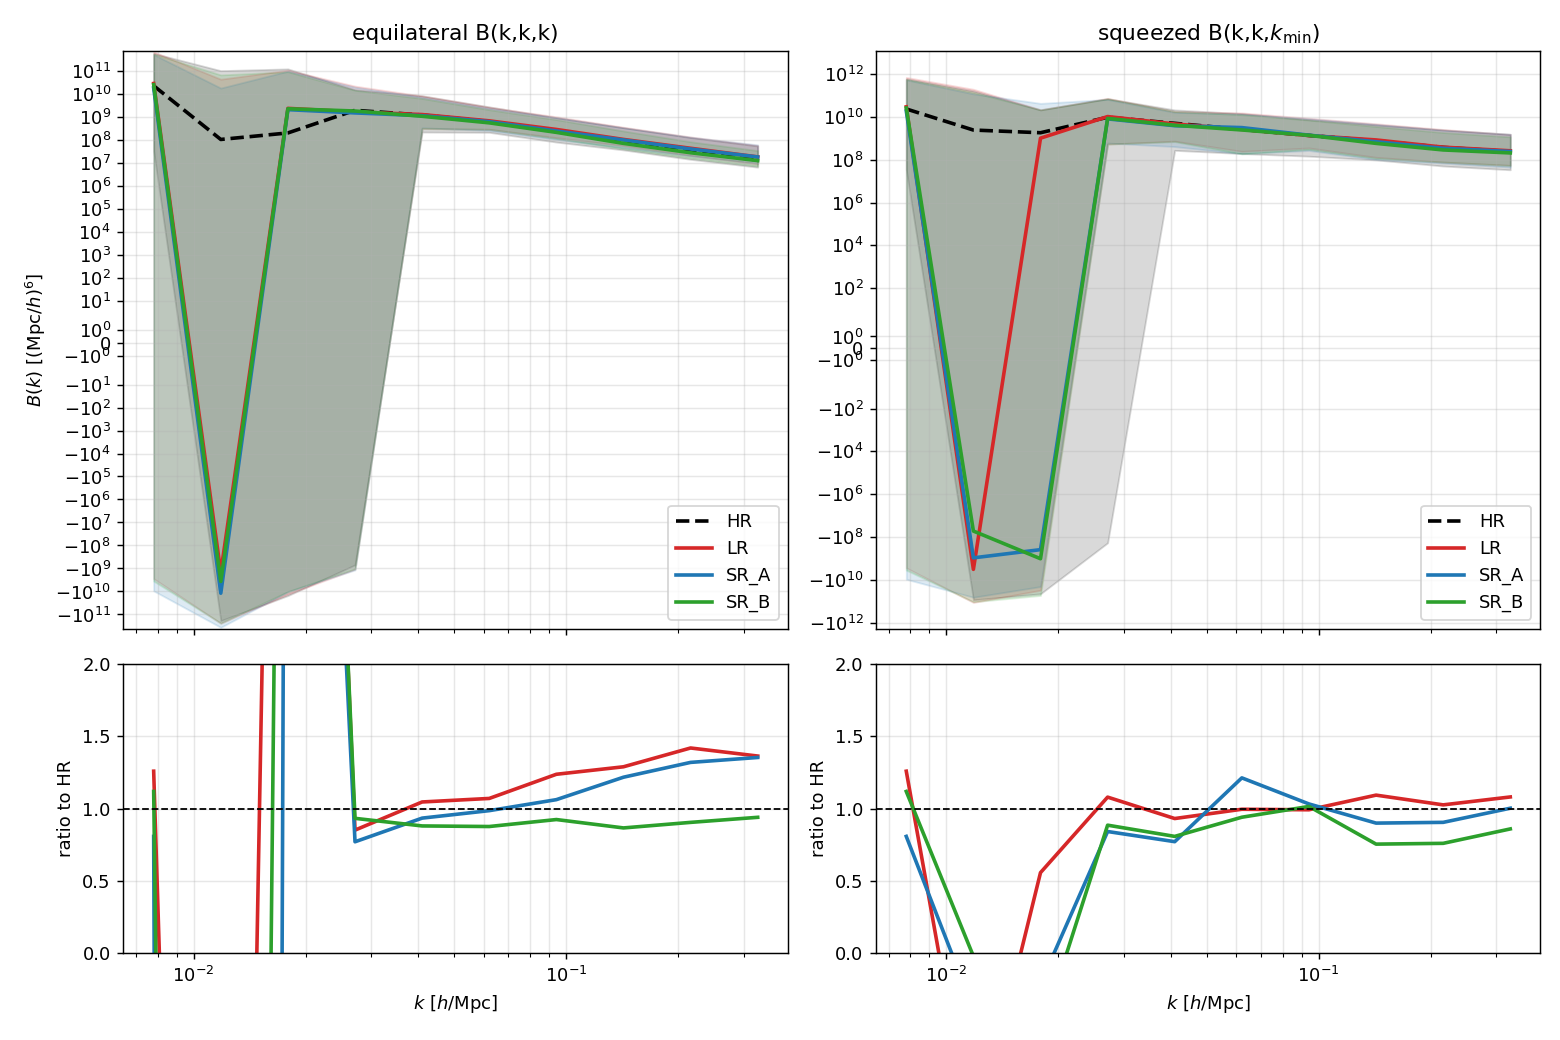
\includegraphics[width=0.95\linewidth]{figures_cmass/bispectrum_hr_lr_srA_srB.png}
\caption{Bispectrum of HR, LR, and SR (both arms), on $16$ test boxes. Top:
equilateral and squeezed bispectrum, HR in black. Bottom: ratio to HR. SR
removes most of the systematic excess that LR has at the plotted scales,
without ever training on this statistic.}
\label{fig:srs-bispec}
\end{figure}

On the equilateral configuration, LR sits about $6$ to $13$ percent above HR
across the middle range of scales. SR removes most of this gap without ever
seeing a bispectrum during training, and it does this for both arms. This is
evidence that the model is not simply fitting the training metric. It is
correcting real structure in the field that also shows up in a statistic it
never saw. (The figure uses the earlier models trained \emph{with} the power
spectrum loss; the no-Pk models of the following paragraphs preserve the
bispectrum at least as well, so removing that loss did not degrade this
held-out statistic either.)

\paragraph{Removing the power spectrum loss.} Following the meeting, we
retrained the model with the power spectrum term switched off
($\lambda_\text{pk}{=}0$ in Eq.~\ref{eq:srs-lossG}), so the loss is only the
adversarial and $L_1$ terms. We also changed which checkpoint counts as "best"
to the real-space $L_1$ error, since selecting on the power spectrum would
have been the same kind of leak we were trying to remove.

\begin{figure}[t]
\centering
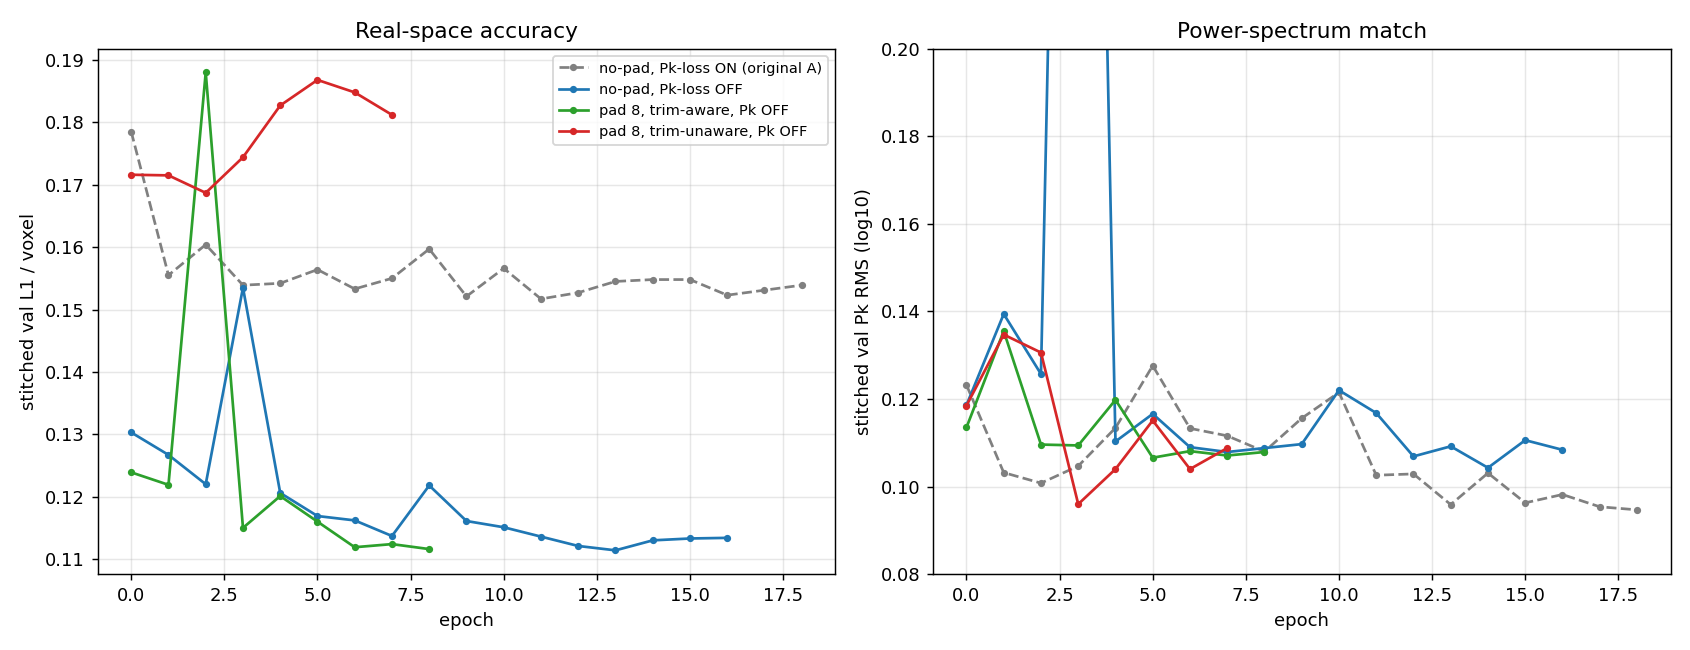
\includegraphics[width=0.98\linewidth]{figures_cmass/protocolv2_cmass.png}
\caption{Stitched validation curves under the new protocol (power spectrum
loss off). Left: real-space $L_1$ error. Right: power spectrum RMS error. Grey
dashed: the original Arm A with the power spectrum loss on, for comparison.
These runs are still training; curves stop at the most recent completed
epoch.}
\label{fig:srs-protocolv2}
\end{figure}

Two things stand out so far. First, without the power spectrum term, the
real-space $L_1$ error becomes clearly better than the original run at the
same point in training (left panel, blue and green curves sit below the grey
dashed curve). Second, the power spectrum error does get a little worse
without its loss term, but it does not collapse: it settles into roughly the
same range as before, just a bit noisier. So the power spectrum term was
buying us a small amount of power spectrum accuracy at a real cost in
real-space accuracy. It was not the only reason the power spectrum matched
well; the adversarial and reconstruction terms carry most of that on their
own.

\paragraph{Does padding help, once the power spectrum loss is out of the way?}
The report above found that padding (Arm B) did not beat no padding (Arm A) on
the power spectrum. The mentor pointed out two different ways this could
happen, and that they make different, testable predictions:
\begin{itemize}
  \item \textbf{Trim-aware.} The model is trained knowing that only the middle
  part of its output will be kept; the loss only looks at that middle part.
  This is what Arm B already did. If this is working correctly, padding should
  train at least as well as no padding, since it has strictly more context for
  the same target.
  \item \textbf{Trim-unaware.} The model is trained as if its whole padded
  output matters, including the edge region that gets thrown away later. If
  the model leans on that edge region during training, it should look fine
  during training but generalize worse once the edge is cut off at test time.
\end{itemize}
We trained both versions with the power spectrum loss off, so the comparison
is not confused by that term. Figure~\ref{fig:srs-protocolv2} shows all three
runs together (no padding, trim-aware padding, trim-unaware padding).

The trim-aware version (green) matches or beats no-padding (blue) on both
real-space error and power spectrum error at almost every epoch measured so
far. This supports the first prediction: once the model is told correctly what
part of its output is graded, more context helps rather than hurts. The
trim-unaware version (red) is clearly worse on real-space error than both
other runs, and does not close that gap as training continues. This supports
the second prediction: a model that is allowed to rely on the part of its
output that gets discarded at test time pays for that at test time. Put
together, the original result that padding did not help was most likely
caused by the power spectrum loss, not by padding itself.

We also reran the older, padding-with-power-spectrum-loss model for more
epochs to check whether it had simply not been trained long enough. Fifteen
additional epochs did not beat its early best score, so that run was not
undertrained; the training recipe, not the training time, was the limiting
factor.

\subsection{The Goal Metric: Corrected Cross-Fidelity Results}
\label{sec:srs-correction}

\paragraph{The bug.} After the analysis above, a routine physical sanity check
failed in a way that could not be real: the amplitude of the power spectrum had
essentially zero correlation with $\sigma_8$, and a fit of the power spectrum to
the five parameters explained only $0.2\%$ of the variance. The power spectrum
amplitude must scale with $\sigma_8$, so this pointed to a labeling error, not to
physics. Tracing it, we found that the processed count fields were written in
string-sorted simulation order ($0, 1, 10, 100, 1000, \dots$) while the cosmology
table is indexed numerically. Field number $k$ is therefore the halo field of
simulation string-sort$(k)$, not simulation $k$, so every field in the whole
pipeline was paired with the wrong cosmology. We proved this exactly: using the
original halo catalogs, the field halo count matches the catalog count under the
string-sort permutation for all $2000$ simulations, while the identity mapping
matches only the two fixed points. We corrected the cosmology table to field
order, backed up the old one, and patched the builder so it cannot regenerate the
wrong order.

\begin{figure}[h]
\centering
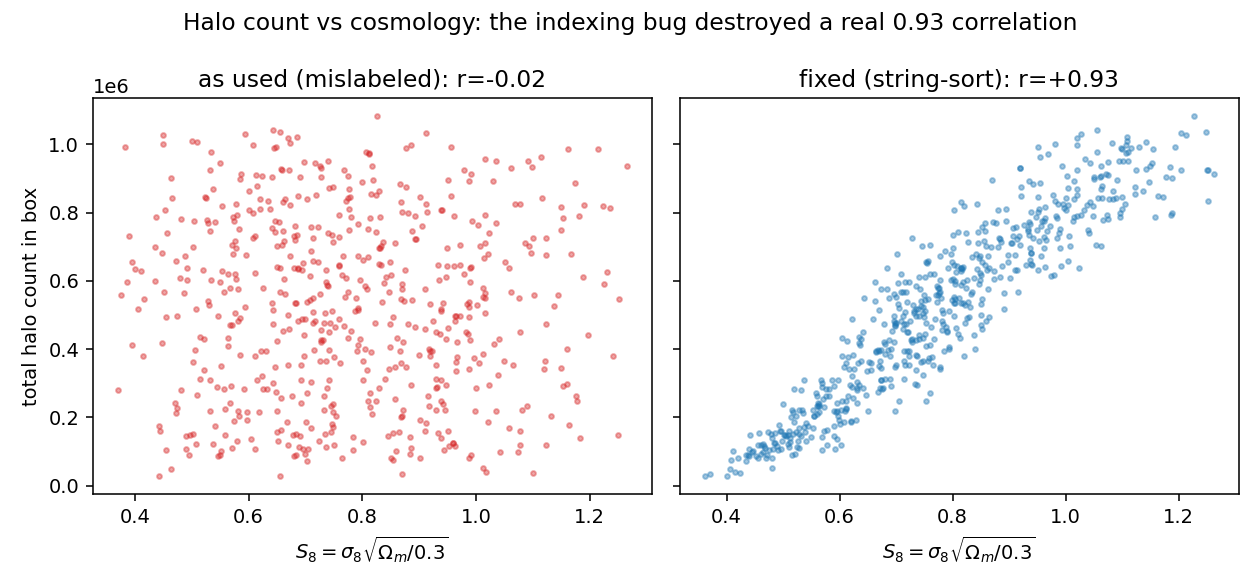
\includegraphics[width=0.85\linewidth]{figures_cmass/labelbug_count_vs_s8.png}
\caption{The indexing bug in one picture. Total halo count in a box against
$S_8 = \sigma_8\sqrt{\Omega_m/0.3}$. As the pipeline used the labels (left) the
correlation is zero; with the string-sort mapping corrected (right) the true
$0.93$ correlation reappears. Halo abundance must track $S_8$, so the left panel
was the signature of a labeling error, not of uninformative data.}
\label{fig:srs-labelbug}
\end{figure}

\paragraph{What this changes, and what it does not.} Every cosmology number we
computed before this point used the labels and is affected; the earlier
cross-fidelity tables have been removed and are replaced by the corrected results
below, and the earlier reading that the SR-versus-LR difference was an irreducible
coin flip was itself a product of the mislabeling. The results that do not use the
labels are unaffected and still stand: the power spectrum match of SR to HR, the
held-out bispectrum, the field-match statistics, the seam test, and the real space
error. The generator conditions on the cosmology as a style vector and was trained
with the scrambled labels, so its conditioning was uninformative during training;
we return to this at the end.

\paragraph{The data is informative after all.} With correct labels the picture
inverts. A halo count in this suite carries a strong cosmological signal: the
total halo count alone correlates with the combination $S_8 = \sigma_8
\sqrt{\Omega_m/0.3}$ at $0.93$ and with $\Omega_m$ at $0.85$. A Fisher forecast on
a single-box power spectrum now explains $98\%$ of the variance, where it
explained $0.2\%$ before, and it constrains $\Omega_m$ and $\sigma_8$ well, with
$\Omega_b$, $h$ and $n_s$ weak or unconstrained, which is the textbook pattern for
a low-redshift halo field. The field-level network tells the same story: after the
fix its predicted $\Omega_m$ correlates with the truth at $0.90$ on both training
and test boxes, where before the fix the correlation was zero and the output was a
constant. So the earlier conclusion that a single box carries almost no cosmology
was an artifact of the labeling, not a property of the data.

\begin{figure}[h]
\centering
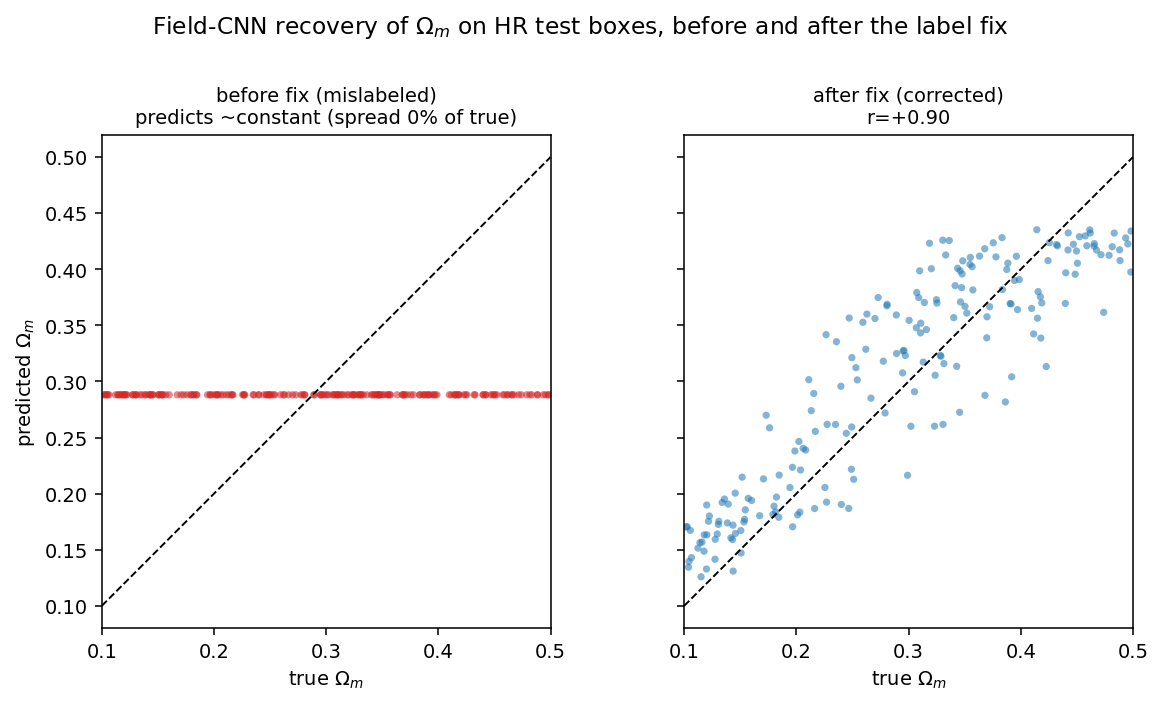
\includegraphics[width=0.82\linewidth]{figures_cmass/field_recovery_Om_cmass.png}
\caption{Field-level CNN recovery of $\Omega_m$ on HR test boxes, before and after
the label fix. Before (left) the prediction is flat and uncorrelated with the
truth (the network returns a near-constant); after (right) it tracks the diagonal
at a correlation of about $0.90$, on both training and test boxes. Same
architecture, same data, only the labels changed.}
\label{fig:srs-recovery}
\end{figure}

\begin{figure}[h]
\centering
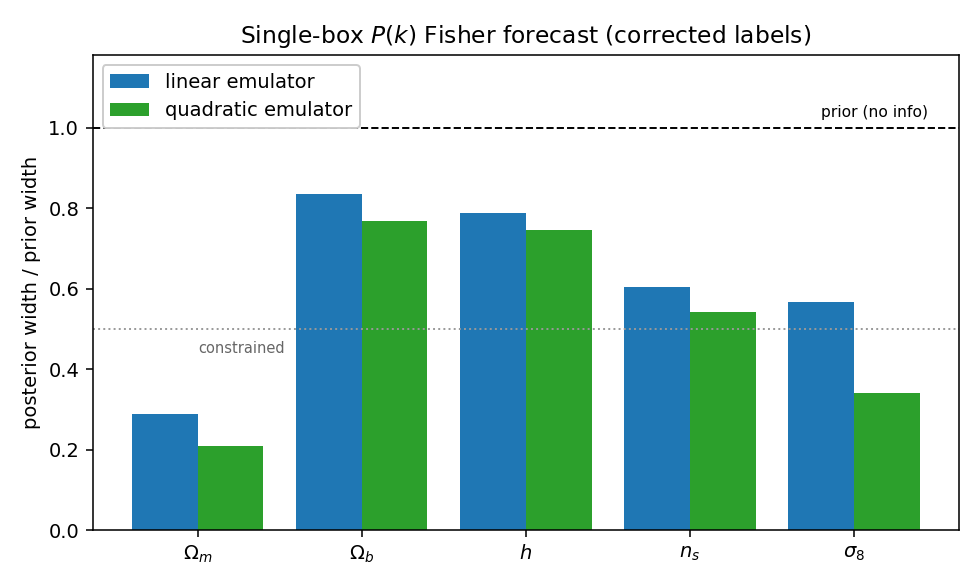
\includegraphics[width=0.72\linewidth]{figures_cmass/fisher_corrected_cmass.png}
\caption{Fisher forecast for a single-box power spectrum with corrected labels:
posterior width divided by prior width per parameter (lower means better
constrained, $1$ means no information). $\Omega_m$ is well constrained and
$\sigma_8$ is constrained, while $\Omega_b$, $h$ and $n_s$ are weak, the textbook
pattern for a low-redshift halo field. Two emulators (linear average slope and
quadratic at the prior centre) bracket the estimate.}
\label{fig:srs-fisher}
\end{figure}

\paragraph{Corrected cross-fidelity, and where SR helps.} We re-ran the goal
metric with correct labels at two levels, the power spectrum summary and the full
field. We train the posterior on one source, apply it to HR, and compare to a
posterior trained on HR, using an ensemble of independently retrained estimators
so the numbers are not single draws. Table~\ref{tab:srs-corrected} gives the
result.
\begin{table}[h]
\centering
\caption{Corrected cross-fidelity KL to HR (posterior trained on the named source,
evaluated on HR), lower is better, with the HR-to-HR floor for reference. Summary
uses the power spectrum; field uses a three-dimensional CNN posterior on the full
box.}
\label{tab:srs-corrected}
\begin{tabular}{lccc}
\toprule
level & LR (raw) & SR & HR floor \\
\midrule
summary $P(k)$ & $0.032$ & $0.088$ & $0.028$ \\
field (CNN)    & $0.49 \pm 0.81$ & $\mathbf{0.024}$ & $0.022$ \\
\bottomrule
\end{tabular}
\end{table}
\begin{figure}[h]
\centering
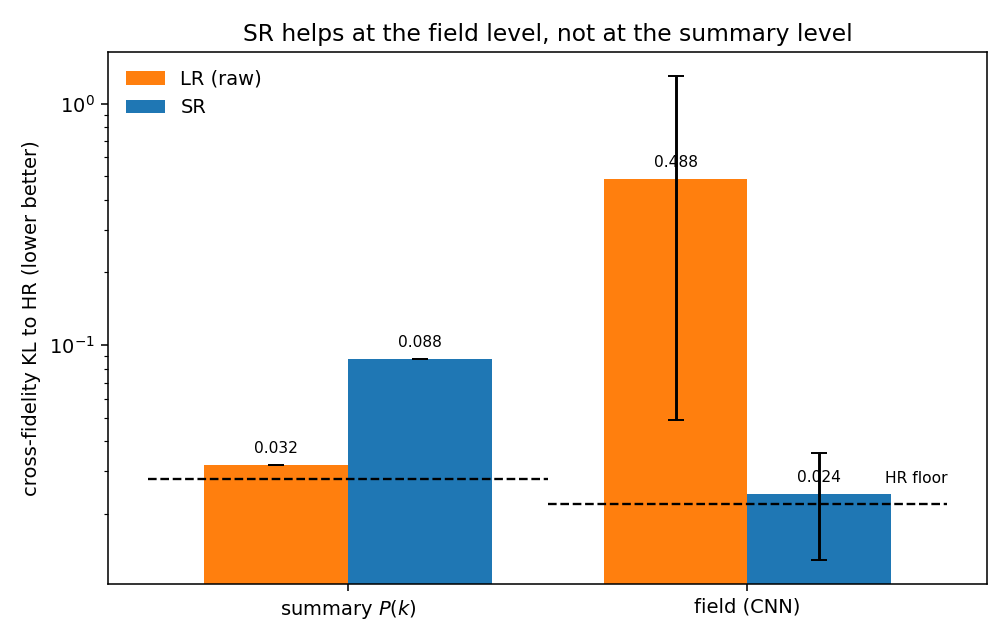
\includegraphics[width=0.7\linewidth]{figures_cmass/crossfid_corrected_cmass.png}
\caption{Corrected cross-fidelity KL to HR (log scale, lower is better) at the two
levels, with the HR-to-HR floor shown as the dashed line. At the summary level the
raw LR field is already at the floor and SR does not help. At the field level, an
LR-trained posterior does not transfer to HR (large and unstable), while an
SR-trained posterior sits at the floor. SR helps exactly where it corrects the
field.}
\label{fig:srs-crossfid-corrected}
\end{figure}
The two levels point in opposite directions, and both make sense. At the summary
level the raw LR power spectrum is already at the HR floor, so an LR-trained
posterior transfers to HR as well as an HR-trained one does, and there is no gap
for SR to close; SR even hurts a little, because the generator reshapes the
small-scale power in a way that does not match how HR responds to cosmology. At
the field level the raw LR box looks different enough from HR that an LR-trained
posterior does not transfer, and it does so unreliably, sometimes acceptably and
sometimes catastrophically, which is why its number carries such a large spread.
SR corrects the field to look like HR, so an SR-trained posterior transfers to HR
reliably, at the floor. This is exactly the deployment case the project is built
on, train the inference model on cheap SR-corrected boxes and apply it to
expensive HR, and at the field level SR makes it work where raw LR does not.

\paragraph{Padding on the goal metric.} We ran the two padding variants through
the corrected cross-fidelity at the summary level as well
(Table~\ref{tab:srs-padding}). Among the SR models the ordering from the earlier
report survives: no padding is best on the goal metric, trim-aware padding is
worse, and trim-unaware is worst, so for the cosmology objective the no-padding
model is the one to use. All three sit above the raw LR control at this level,
consistent with LR already being HR-like on the power spectrum. One number does
change under the fix: the mislabeled data made trim-unaware look catastrophic (a
factor of several hundred above the others), while with correct labels it is the
weakest variant by about a factor of two, not a blow-up. Its real-space error
(Figure~\ref{fig:srs-protocolv2}) remains the clearest and most direct sign that
it is the least reliable model.
\begin{table}[h]
\centering
\caption{Corrected cross-fidelity KL to HR at the summary (power spectrum) level
for the SR padding variants, with the LR control and the HR floor. Lower is
better. Field-level padding numbers are future work.}
\label{tab:srs-padding}
\begin{tabular}{lc}
\toprule
model & summary cross-fidelity KL \\
\midrule
SR, no padding & $\mathbf{0.087}$ \\
SR, trim-aware padding & $0.127$ \\
SR, trim-unaware padding & $0.172$ \\
\midrule
LR (control) & $0.031$ \\
HR floor & $0.028$ \\
\bottomrule
\end{tabular}
\end{table}

\paragraph{Bottom line.} With the labels fixed, the cosmology question has a
clear answer. The data constrains $\Omega_m$ and $\sigma_8$ from a single box. At
the power spectrum level the raw LR field is already HR-like, so SR is not needed
there and slightly hurts. At the field level, which is what SR actually corrects,
an SR-trained posterior transfers to HR at the floor while a raw LR one does not,
so SR provides a real and reliable cosmology benefit exactly where it operates.
Trim-unaware padding is still the weakest variant, worst on the goal metric and
on real-space error, though the label fix shrinks its apparent failure from
catastrophic to about a factor of two. Two honest caveats remain: the
field-level LR number has a wide spread and rests on a handful of retrained
networks, so the size of the gap should be firmed up with more seeds; and because
the generator was trained with the scrambled labels, its cosmology conditioning
was uninformative, so a retrain with correct conditioning may sharpen the SR
result further. Neither caveat changes the direction: with correct labels, SR
helps cosmology at the field level.

\paragraph{A data reliability note.} Partway through these runs, the shared
data storage this project reads from filled up completely, which caused a few
training jobs to fail with a file briefly appearing missing even though it was
not actually deleted. We added a retry step to the data loader and resumed
each affected run from its last saved checkpoint, so no real training progress
was lost. This is a shared infrastructure issue, not a problem with the data or
the method.

\subsection{Files}
\begin{itemize}\itemsep0pt
  \item Data and patching: \texttt{data/patch\_dataset\_cmass.py}
  (shared ops in \texttt{data/patch\_dataset\_real.py})
  \item Model: \texttt{map2map/models/styled\_srsgan.py}
  (\texttt{G\_correct}, \texttt{D\_const})
  \item Training: \texttt{train\_patch\_cmass.py};
  run script \texttt{scripts/train\_patch\_cmass.slurm}
  \item Inference and stitching: \texttt{infer\_stitch\_cmass.py}
  \item Seam eval: \texttt{analysis/eval\_seam\_cmass.py}
  \item Box / per-patch diagnostics: \texttt{analysis/diag\_cmass.py}
  \item SR-vs-HR match stats: \texttt{analysis/match\_stats\_cmass.py}
  \item SR-vs-HR power-spectrum figure: \texttt{analysis/plot\_sr\_vs\_hr.py}
  \item Bispectrum (held-out statistic): \texttt{analysis/bispectrum\_cmass.py}
  \item Training loss curves: \texttt{analysis/plot\_losses\_cmass.py}
  \item Cross-fidelity posterior evaluation: \texttt{evaluate.py} (SR-trained
  or LR-trained posterior evaluated on HR $P(k)$)
  \item Protocol-v2 (no-Pk-loss, padding-variant) training curves:
  \texttt{analysis/plot\_protocolv2\_cmass.py}
  \item Power spectrum on counts: \texttt{analysis/power\_spectrum.py}
  (estimator \texttt{counts}); differentiable training version
  \texttt{analysis/pk\_torch.py}
  \item Posterior and KL: \texttt{inference/nde.py}, \texttt{evaluate.py};
  end-to-end eval \texttt{scripts/eval\_cmass\_wrapper.slurm}
  \item Field-level posterior (three-dimensional CNN, moment-network loss):
  \texttt{models/field\_cnn.py}, \texttt{train\_field\_cnn.py};
  SR field generation \texttt{gen\_sr\_fields.py}; capacity and recovery
  diagnostics \texttt{overfit\_test.py}, \texttt{field\_diag.py}
  \item Outputs: \texttt{runs/patch\_cmass/}; figures: \texttt{figures\_cmass/}
\end{itemize}
 from main.tex, or paste inline.
% Figures referenced live in figures_cmass/ (set \graphicspath or copy them
% next to main.tex). Every number is from runs/patch_cmass/ and FINAL.md.
% =====================================================================

\section{SRS-styled-map2map-galaxy}
\label{sec:srs}

This section documents the second model in this work at the same level of
detail as \S5. Where \S5 corrects a Lagrangian \emph{displacement} field with a
point--voxel flow matcher, this model corrects an Eulerian \emph{halo count}
field with a styled GAN. The two share the same high-level goal, make a cheap
low-fidelity (LF) simulation look like an expensive high-fidelity (HF) one, 
but operate on different data and use a different architecture.

\paragraph{Goal.} Running an accurate (high-resolution) N-body simulation is
expensive; running a fast approximate one is cheap. We want a model that takes
\emph{only} the cheap LF field and produces a corrected field (we call it the
super-resolved or \textbf{SR} field) that matches the expensive HF field. At
inference the model never sees HF: the HF field is used only to train the model
and to grade it. So every result in this section answers one question: \emph{how
close is the SR field, built from LF alone, to the HF field it never saw?}

\paragraph{Terminology.} We work one cubic sub-volume at a time. We call the
$64^3$ output sub-volume a \textbf{core}, and the (possibly larger) input
sub-volume that the model reads a \textbf{patch}. When \texttt{pad}${=}0$ the
patch and the core coincide. We use \textbf{LR}/\textbf{LF} and
\textbf{HR}/\textbf{HF} interchangeably; the data here is named LR (input) and
HR (target).

\paragraph{Two arms.} We test the boundary treatment with two arms that are
identical except for one number:
\begin{itemize}
  \item \textbf{Arm A (naive, mentor 2.1):} \texttt{pad}${=}0$. Each $64^3$ core
  is corrected and placed edge-to-edge.
  \item \textbf{Arm B (overlap, mentor 2.2):} \texttt{pad}${=}8$. Each patch is
  grown to $80^3$ with real neighbour cells (periodic wrap), only the central
  $64^3$ core is kept and placed.
\end{itemize}

\subsection{Data Preprocessing}
\textit{Source: \texttt{cmass-ili}; loader \texttt{data/patch\_dataset\_cmass.py}.}

\paragraph{Input.} We have $2000$ paired simulations at redshift $z=0.5$, run
from shared initial conditions. Each pair is a low-fidelity field (LR, from the
FastPM particle-mesh code) and a high-fidelity field (HR, from a Quijote N-body
run). Both are stored as integer \textbf{halo count grids} of shape
$128\times128\times128$ on a periodic box of side $L_\text{box}=1000\
\mathrm{Mpc}/h$ (cell size $\approx 7.81\ \mathrm{Mpc}/h$). A cell value is the
number of halos whose position falls in that cell. The fields are sparse: most
cells are zero and the mean count per cell is small (the code caches one global
count scale, the mean HR count per cell measured over $50$ training sims).
Because LR and HR share initial conditions, they describe the same structure at
two fidelities. The correspondence is between the two halo catalogs \emph{as a
whole}: there is no known one-to-one matching between individual LR and HR
halos, only between the count fields they produce.

\paragraph{Cosmology labels.} Each simulation carries a style vector
$\mathbf s=(\Omega_m,\Omega_b,h,n_s,\sigma_8)\in\mathbb R^5$, parsed from that
sim's \texttt{config.yaml}.

\paragraph{Splits.} The on-disk lists give $1600$ train, $200$ validation, and
$200$ test simulations, split by simulation index.

\begin{figure}[t]
\centering
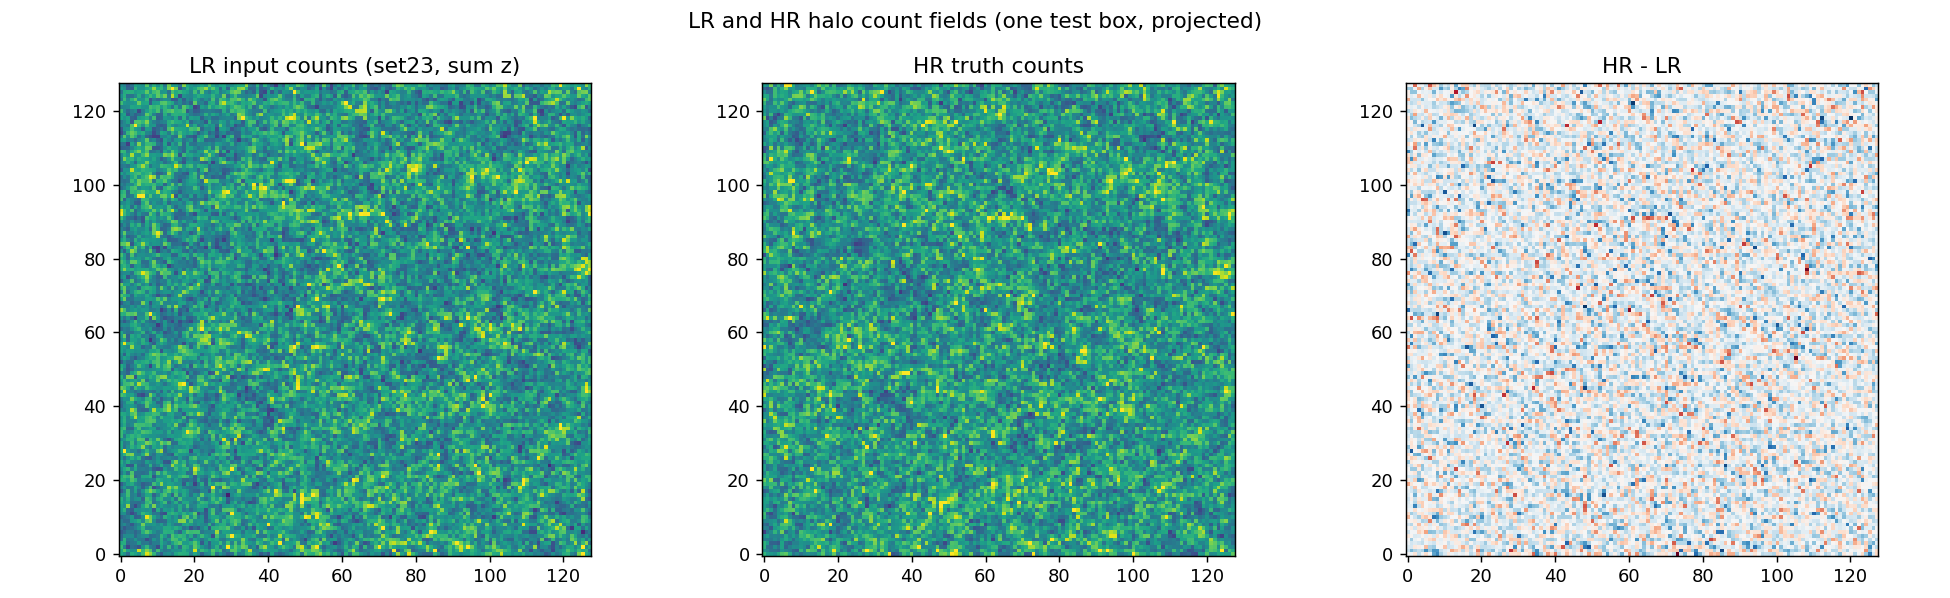
\includegraphics[width=0.9\linewidth]{figures_cmass/data_pair.png}
\caption{One LR/HR pair (projected count map). LR (FastPM, input) and HR
(Quijote N-body, target) share initial conditions and so share large-scale
structure, but differ cell-by-cell.}
\label{fig:srs-datapair}
\end{figure}

\paragraph{Model space (count transform).} The network does not learn on raw
counts; it learns in a compressed ``model space''. The default transform is
$\log(1+n)$, which tames the sparse heavy tail:
\begin{equation}
  y = \log(1+n), \qquad n = \exp(y)-1 \ \ (\text{clamped to } n\ge 0).
  \label{eq:srs-transform}
\end{equation}
Two alternative transforms exist in the code (\texttt{scale}: $n/\text{scale}$;
\texttt{delta}: model space is the overdensity itself), but all reported runs use
$\log(1+n)$. Power spectra are \emph{never} computed in model space; they are
always computed on the physical-count overdensity \SG{Is it okay if this is -1 when there are 0 halos?}
\begin{equation}
  \delta = \frac{n}{\bar n} - 1,
  \label{eq:srs-delta}
\end{equation}
with $\bar n$ the per-box mean count (the \texttt{perbox} setting used in all
runs).

\subsection{Data Pipeline (patching)}
\textit{Located in: \texttt{data/patch\_dataset\_cmass.py},
\texttt{data/patch\_dataset\_real.py} (shared patch ops).}

A model never sees the whole $128^3$ box at once. We cut the box into a
$2\times2\times2$ grid of $64^3$ \textbf{cores} (Table~\ref{tab:srs-notation}).
The cores tile the box exactly (stride $64$), so they reconstruct the box
bit-for-bit with no gaps and no double counting, the dataset's self-test
asserts this. Each model \emph{input} is a core grown by \texttt{pad} voxels on
every side, taken from the true neighbour cells with periodic wrap at the box
edge (\texttt{extract\_patch} uses \texttt{numpy.take(\dots, mode="wrap")}). So
with \texttt{pad}${=}8$ the input is $80^3$ and neighbouring patches overlap by
$2\cdot\texttt{pad}=16$ voxels; the HR \emph{target} is always the bare $64^3$
core. Because each simulation is one continuous periodic box that we crop
ourselves, the patches are real neighbours by construction, there is no data
seam (unlike the Lagrangian patches of \S5). \SG{Isn't the patch construction same in both?}

\begin{table}[t]
\centering
\caption{Notation for the CMASS count-field pipeline.}
\label{tab:srs-notation}
\begin{tabular}{llp{7.2cm}}
\toprule
Symbol & Value & Meaning \\
\midrule
$N_\text{full}$    & $128$ & full box side (voxels) \\
$P$ (\texttt{PATCH}) & $64$ & core side (voxels) \\
$N_\text{patches}$ & $8$ & cores per box ($2{\times}2{\times}2$) \\
\texttt{pad}       & $0$ (Arm A) / $8$ (Arm B) & halo width added to each face by periodic wrap \\
$L_\text{box}$     & $1000\ \mathrm{Mpc}/h$ & box side \\
$\mathbf s$        & $\in\mathbb R^5$ & cosmology vector $(\Omega_m,\Omega_b,h,n_s,\sigma_8)$ \\
$\bar n$           & per-box mean & mean count used to form $\delta=n/\bar n-1$ \\
\bottomrule
\end{tabular}
\end{table}

\begin{figure}[t]
\centering
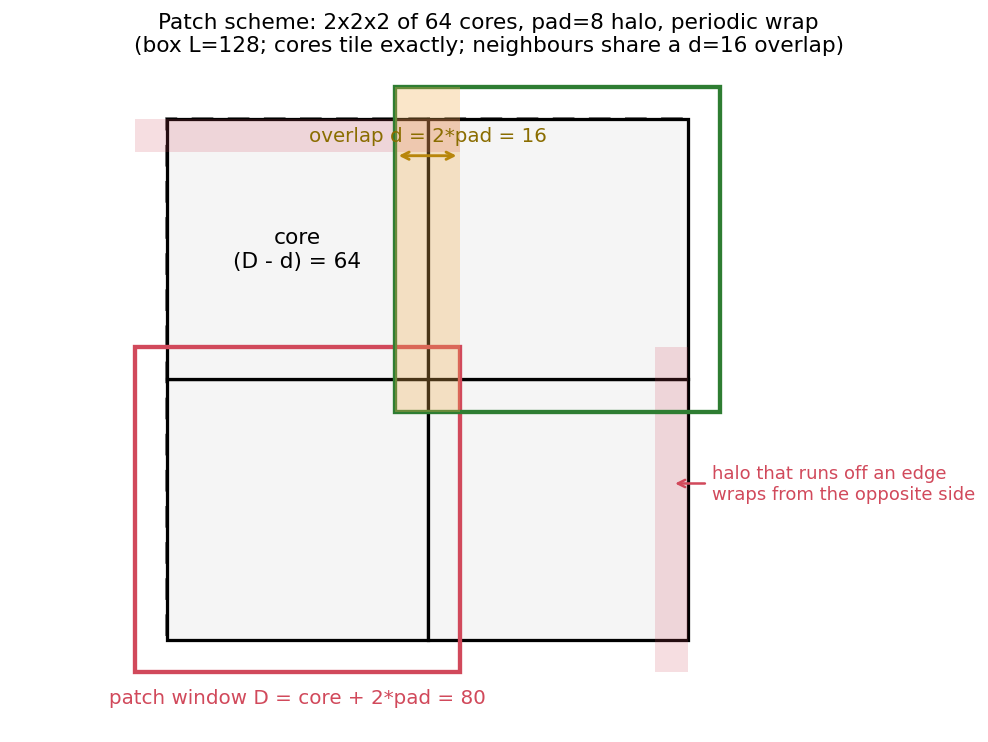
\includegraphics[width=0.82\linewidth]{figures_cmass/pipeline_patching.png}
\caption{Patch scheme. The box is cut into a $2{\times}2{\times}2$ grid of
$64^3$ cores that tile it exactly. With \texttt{pad}${>}0$ each patch is grown by
a halo of real neighbour cells (periodic wrap); only the central core is kept
and placed back.}
\label{fig:srs-patching}
\end{figure}

\paragraph{Per-simulation item.} Indexed by simulation, the dataset returns, for
all $8$ cores at once: the LR patches \texttt{lr\_in} of shape
$(8,\,1,\,64{+}2\,\texttt{pad},\,\cdot,\,\cdot)$ in model space, the HR cores
\texttt{hr\_tgt} of shape $(8,\,1,\,64,\,64,\,64)$, the style $\mathbf s$, and
the simulation index. The trainer flattens the $8$-core axis into the batch.

\begin{algorithm}[H]
\caption{\textsc{ExtractPatches} (one simulation)}
\label{alg:srs-extract}
\begin{algorithmic}[1]
\Require LR box $\mathbf L\in\mathbb R^{1\times128^3}$, HR box $\mathbf H$, \texttt{pad}
\State map $\mathbf L,\mathbf H$ to model space via Eq.~\ref{eq:srs-transform}
\For{$p=0,\dots,7$}
  \State $(i,j,k)\gets\textsc{unravel}(p,(2,2,2))$ \Comment{core origin $(64i,64j,64k)$}
  \State $\mathbf L_p\gets$ core $p$ grown by \texttt{pad} on each face, periodic wrap \Comment{$(64{+}2\,\texttt{pad})^3$}
  \State $\mathbf H_p\gets$ bare core $p$ \Comment{$64^3$}
\EndFor
\State \Return $\{(\mathbf L_p,\mathbf H_p)\}_{p=0}^{7}$, style $\mathbf s$
\end{algorithmic}
\end{algorithm}

\subsection{Model: Input/Output Specification}
\textit{Implementation: \texttt{map2map/models/styled\_srsgan.py}
(\texttt{G\_correct}, \texttt{D\_const}).}

\paragraph{What the generator computes.} The generator is a
\textbf{same-resolution residual} network: it does not change the grid size, and
it predicts a correction that is \emph{added} to the input. In model space,
\begin{equation}
  \mathrm{SR} \;=\; \mathrm{LR} \;+\; G(\mathrm{LR},\,\mathbf s,\,\mathbf z),
  \label{eq:srs-residual}
\end{equation}
where $\mathbf s$ is the cosmology vector and $\mathbf z$ is an injected noise
field (see below). Inputs and outputs are listed in
Table~\ref{tab:srs-model-io}; the generator is run once per core (the $8$ cores
of a box form a batch).

\begin{table}[t]
\centering
\caption{Tensors consumed/produced by the generator \texttt{G\_correct} for one
core (batch dimension omitted). Here $D=64{+}2\,\texttt{pad}$.}
\label{tab:srs-model-io}
\begin{tabular}{lll}
\toprule
Symbol & Shape & Meaning \\
\midrule
$\mathbf x$ (\texttt{x})       & $(1,D,D,D)$ & LR patch, model space (input) \\
$\mathbf s$ (\texttt{style})   & $(5,)$      & cosmology vector \\
$\mathbf z$ (\texttt{noise\_list}) & $2\cdot\texttt{num\_blocks}$ cubes $(1,D,D,D)$ & injected noise; fixed at inference, random in training \\
$G(\cdot)$                     & $(1,D,D,D)$ & predicted residual $\delta$ (added to $\mathbf x$) \\
\bottomrule
\end{tabular}
\end{table}

\paragraph{Internal composition.} $G$ is a constant-resolution StyleGAN2-style
network (no up/down-sampling), built from:
\begin{enumerate}
  \item \texttt{block0}: a $1{\times}1{\times}1$ style-modulated convolution
  (\texttt{ConvStyled3d}) lifting the $1$-channel input to $c_0$ channels,
  followed by a leaky ReLU.
  \item \texttt{num\_blocks} ($=4$) constant-resolution H-blocks
  (\texttt{HBlock\_const}). Each block, in order: inject noise $\to$
  $3{\times}3{\times}3$ \texttt{ConvStyled3d} (periodic ``circular'' padding)
  $\to$ leaky ReLU $\to$ inject noise $\to$ $3{\times}3{\times}3$
  \texttt{ConvStyled3d} $\to$ leaky ReLU $\to$ a $1{\times}1{\times}1$ projection
  to the output channel, accumulated into a running output $y$. The final return
  is $\mathbf x + y$ (Eq.~\ref{eq:srs-residual}).
\end{enumerate}
The channel widths come from \texttt{chan\_base} ($=128$) halved per block and
clamped to $[64,512]$. Two mechanisms make the convolutions depend on side
information:
\begin{itemize}
  \item \textbf{Style modulation.} \texttt{ConvStyled3d} is the StyleGAN2
  modulated/demodulated convolution: the cosmology vector $\mathbf s$ scales the
  convolution weights, so the same network behaves differently for different
  cosmologies. This is the only path by which $\mathbf s$ enters.
  \item \textbf{Noise injection.} Each \texttt{ConvStyled3d} is preceded by a
  per-channel learned-standard-deviation noise add (\texttt{\_NoiseInject}). At
  training time the noise is fresh Gaussian each call; at inference a
  \emph{fixed} list of noise cubes (seeded, built by \texttt{build\_noise\_list})
  is reused so outputs are reproducible. The noise is what lets the model produce
  a plausible small-scale field rather than a single blurred guess.
\end{itemize}

\paragraph{Discriminator.} \texttt{D\_const} is a constant-input-resolution
critic conditioned on the same style $\mathbf s$. It runs a head
\texttt{ConvStyled3d} then \texttt{num\_blocks} strided down-blocks (each a
periodic $3{\times}3{\times}3$ \texttt{ConvStyled3d} $+$ leaky ReLU $+$
$2{\times}$ average pool), a $1{\times}1{\times}1$ tail, and a final
$1{\times}1{\times}1$ projection to one channel, averaged over space to a single
logit per core.

\subsection{Training Step}
\textit{Located in: \texttt{train\_patch\_cmass.py}.}

The generator is trained per core (stitching is \emph{not} part of the
gradient). The total generator loss is a weighted sum of three terms,
\begin{equation}
  \mathcal L_G \;=\; \lambda_\text{adv}\,\mathcal L_\text{adv}
                  + \lambda_\text{rec}\,\mathcal L_\text{rec}
                  + \lambda_\text{pk}\,\mathcal L_\text{pk},
  \label{eq:srs-lossG}
\end{equation}
with (defaults from the original run script; see the protocol update below for
the values now in use):
\begin{itemize}
  \item \textbf{Reconstruction} $\mathcal L_\text{rec}=\lVert \mathrm{SR}-\mathrm{HR}\rVert_1$,
  a plain $L_1$ in model space (optionally Gaussian-smoothed; smoothing off in
  all runs).
  \item \textbf{Power-spectrum} $\mathcal L_\text{pk}$, the mean-squared error
  between the $\log_{10}$ power spectra of SR and HR, computed on the
  \emph{physical-count overdensity} of the $64^3$ core (Eqs.~\ref{eq:srs-transform}--\ref{eq:srs-delta}),
  Hann-windowed, with the HR side detached:
  \begin{equation}
    \mathcal L_\text{pk} = \frac{1}{|K|}\sum_{k\in K}
      \big(\log_{10} P_\text{SR}(k) - \log_{10} P_\text{HR}(k)\big)^2 .
    \label{eq:srs-pkloss}
  \end{equation}
  \item \textbf{Adversarial} $\mathcal L_\text{adv}=\mathrm{softplus}\!\big({-}D(\mathrm{SR},\mathbf s)\big)$,
  the non-saturating GAN generator loss.
\end{itemize}

\paragraph{Protocol update: what region the reconstruction and adversarial
terms see.} A \texttt{--pad-loss} setting controls how much of the generator's
output the $L_1$ and adversarial terms are computed on, independent of
\texttt{pad} itself:
\begin{itemize}
  \item \texttt{crop} (trim-aware, the setting used for Arm B above): the loss
  is computed only on \textsc{cropInterior}$(G(\mathbf x,\mathbf s),\,\texttt{pad})$,
  the $64^3$ core that is actually kept at inference time, against the bare
  $64^3$ HR core. The model is trained on exactly the region it will be graded
  on.
  \item \texttt{full}: the loss is computed on the whole $(64{+}2\,\texttt{pad})^3$
  output, against a correspondingly padded HR target (the dataset's
  \texttt{pad\_target} option). The model is trained as if the halo region it
  will later be trimmed off also mattered.
\end{itemize}
Concretely, let $\texttt{loss\_crop}=\texttt{pad}$ under \texttt{crop} and $0$
under \texttt{full}; every place above that writes $\mathrm{SR}$ means
$\textsc{cropInterior}(G(\mathbf x,\mathbf s),\,\texttt{loss\_crop})$, and the
Hann window and $P(k)$ estimator in $\mathcal L_\text{pk}$ are sized to match.
This is a controlled test of two ways padding could fail to help: see the
protocol-update subsection below for the result.

The discriminator is trained with the non-saturating GAN loss plus a lazy $R_1$
gradient penalty applied every \texttt{r1\_every} steps:
\begin{equation}
  \mathcal L_D = \mathrm{softplus}\!\big({-}D(\mathrm{HR})\big)
               + \mathrm{softplus}\!\big(D(\mathrm{SR})\big)
               + \tfrac{1}{2}\lambda_{R_1}\,\mathbb E\big\lVert \nabla_{\!x} D(x,\mathbf s)\big\rVert^2 .
  \label{eq:srs-lossD}
\end{equation}

\begin{algorithm}[H]
\caption{CMASS patch-GAN training step (one batch of cores)}
\label{alg:srs-train}
\begin{algorithmic}[1]
\Require LR patches $\mathbf x$, HR targets $\mathbf h$ (padded iff \texttt{pad-loss=full}),
         style $\mathbf s$, \texttt{pad}, \texttt{loss\_crop} ($=\texttt{pad}$ if \texttt{crop} else $0$),
         weights $\lambda_\text{adv},\lambda_\text{rec},\lambda_\text{pk},\lambda_{R_1}$
\Statex \textbf{// Discriminator}
\State $\hat{\mathbf h}\gets \textsc{cropInterior}\big(G(\mathbf x,\mathbf s),\,\texttt{loss\_crop}\big)$ \Comment{no grad}
\State $\mathcal L_D \gets \mathrm{softplus}({-}D(\mathbf h,\mathbf s)) + \mathrm{softplus}(D(\hat{\mathbf h},\mathbf s))$
\If{step $\bmod\ \texttt{r1\_every} = 0$} $\mathcal L_D \mathrel{+}= \tfrac12\lambda_{R_1}\texttt{r1\_every}\cdot R_1(D,\mathbf h,\mathbf s)$ \EndIf
\State update $D$ (Adam, grad-clip)
\Statex \textbf{// Generator}
\State $\hat{\mathbf h}\gets \textsc{cropInterior}\big(G(\mathbf x,\mathbf s),\,\texttt{loss\_crop}\big)$
\State $\mathcal L_\text{adv}\gets \mathrm{softplus}({-}D(\hat{\mathbf h},\mathbf s))$
\State $\mathcal L_\text{rec}\gets \lVert \hat{\mathbf h}-\mathbf h\rVert_1$
\State $\mathcal L_\text{pk}\gets$ Eq.~\ref{eq:srs-pkloss} on Hann-windowed overdensity of $\hat{\mathbf h}$, $\mathbf h$
       (skip if $\lambda_\text{pk}{=}0$)
\State $\mathcal L_G \gets \lambda_\text{adv}\mathcal L_\text{adv}+\lambda_\text{rec}\mathcal L_\text{rec}+\lambda_\text{pk}\mathcal L_\text{pk}$
\State update $G$ (Adam, grad-clip)
\end{algorithmic}
\end{algorithm}

\paragraph{Validation and checkpoint selection.} After each epoch we stitch the
full $128^3$ SR box for up to $40$ validation sims and report the stitched
$L_1$/voxel and the stitched-$128$ power-spectrum RMS against HR
(\S\ref{sec:srs-eval}, Eq.~\ref{eq:srs-pkrms}). A \texttt{--select} setting
chooses which of the two the saved \texttt{best.pt} tracks: \texttt{pk} (the
original setting, lowest stitched validation Pk RMS) or \texttt{l1} (lowest
stitched validation $L_1$/voxel). Selection is always on the stitched full box,
not the per-core training loss. Runs that also train with $\lambda_\text{pk}{=}0$
use \texttt{--select l1}, since selecting on Pk RMS while not training on it
would reintroduce the same metric leak in a different place.

\subsection{Inference}
\textit{Located in: \texttt{infer\_stitch\_cmass.py}.}

For one simulation: load the LR $128^3$ count box, map it to model space, run $G$
on each of the $8$ cores (with the periodic-wrap halo in Arm B), crop the halo,
stitch the cores into a $128^3$ model-space box, invert the transform to physical
counts, and clamp. \SG{are all outputs later mapped to integers, or are we fine with non-integer number of halos?} The injected noise list is fixed (seeded) so the output is
reproducible.

\begin{algorithm}[H]
\caption{CMASS inference + stitch (one simulation)}
\label{alg:srs-infer}
\begin{algorithmic}[1]
\Require LR box $\mathbf L$, style $\mathbf s$, trained $G$, mode (naive/overlap), fixed noise $\mathbf z$
\State $\texttt{pad}\gets 0$ if naive else value from checkpoint ($8$)
\State map $\mathbf L$ to model space (Eq.~\ref{eq:srs-transform})
\For{$p=0,\dots,7$}
  \State $\mathbf x_p\gets$ patch $p$ (core grown by \texttt{pad}, periodic wrap)
  \State $\mathbf c_p\gets \textsc{cropInterior}\big(G(\mathbf x_p,\mathbf s,\mathbf z),\,\texttt{pad}\big)$ \Comment{$64^3$ core, model space}
\EndFor
\State $\mathbf S\gets \textsc{stitch}(\{\mathbf c_p\})$ \Comment{$128^3$, model space}
\State $\mathbf S\gets \exp(\mathbf S)-1$, clamp to $[0,\,C_\text{max}{=}200]$, replace NaN/Inf \Comment{physical counts}
\State \Return $\mathbf S$
\end{algorithmic}
\end{algorithm}

\subsection{Crop Stitching}

Stitching is \textbf{direct placement with no averaging}. Adjacent cores tile the
box exactly (stride $64$, no overlap between cores once the halo is dropped), so
each core's $64^3$ output is written straight into its slot. In Arm B the $80^3$
patch is corrected and only its central $64^3$ core is kept; the overlap halo is
context for the convolution, never written to the output.

\begin{algorithm}[H]
\caption{\textsc{Stitch} ($8$ cores $\to$ $128^3$)}
\label{alg:srs-stitch}
\begin{algorithmic}[1]
\Require cores $\{\mathbf c_p\}_{p=0}^{7}$, each $1\times64^3$
\State $\mathbf S\gets \mathbf 0\in\mathbb R^{1\times128^3}$
\For{$p=0,\dots,7$}
  \State $(i,j,k)\gets\textsc{unravel}(p,(2,2,2))$
  \State $\mathbf S[:,\,64i{:}64i{+}64,\,64j{:}\cdots,\,64k{:}\cdots]\gets \mathbf c_p$ \Comment{direct assignment}
\EndFor
\State \Return $\mathbf S$
\end{algorithmic}
\end{algorithm}

\subsection{Evaluation}
\label{sec:srs-eval}
\textit{Located in: \texttt{analysis/eval\_seam\_cmass.py},
\texttt{analysis/diag\_cmass.py}, \texttt{analysis/match\_stats\_cmass.py},
\texttt{analysis/power\_spectrum.py}, \texttt{inference/nde.py},
\texttt{evaluate.py}.}

We evaluate the SR field against HR at three levels: a seam check (does stitching
leave a join?), field statistics (does SR have the right structure?), and
cosmology (does SR give the same parameter posterior as HR?).

\paragraph{Power-spectrum summaries.} On the count overdensity (Eq.~\ref{eq:srs-delta})
we report the power spectrum $P(k)$, the transfer ratio, and the cross-coherence:
\begin{equation}
  T(k) = \frac{P_\text{SR}(k)}{P_\text{HR}(k)},
  \qquad
  r(k) = \frac{P_{\text{SR},\text{HR}}(k)}{\sqrt{P_\text{SR}(k)\,P_\text{HR}(k)}} .
  \label{eq:srs-Tr}
\end{equation}
$T(k)=1$ means SR has the right \emph{amount} of power at scale $k$ (amplitude);
$r(k)=1$ means SR has the structure in the right \emph{place} (phase). The
scalar power-spectrum error used for checkpoint selection and seam reporting is
the log-RMS over the resolved $k$-bins:
\begin{equation}
  \mathrm{PkRMS}_{\log_{10}} = \sqrt{\frac{1}{|K|}\sum_{k\in K}
    \big(\log_{10} P_\text{SR}(k) - \log_{10} P_\text{HR}(k)\big)^2 } .
  \label{eq:srs-pkrms}
\end{equation}

\paragraph{Seam diagnostic.} \texttt{eval\_seam\_cmass.py} bins the per-cell
count error $|{\mathrm{SR}-\mathrm{HR}}|$ by distance to the nearest core face
and forms a per-position error profile along each axis. The headline number is
the \textbf{$x{=}64$ internal-seam excess}: the error on the internal core
boundary plane divided by the interior error. A value near $1$ means stitching
leaves no seam. The box edge $x{=}0$ is a periodic-boundary control.

\paragraph{Field-match statistics.} \texttt{match\_stats\_cmass.py} reports, over
$16$ test boxes: the total-count ratio $\sum\mathrm{SR}/\sum\mathrm{HR}$, the
void fraction (cells $<0.5$), the real-space cell standard-deviation ratio
$\mathrm{std}(\mathrm{SR})/\mathrm{std}(\mathrm{HR})$ (a blur check), and the
cross-coherence $r(k)$ at large ($k<0.05$) and small ($k>0.2$) scales.

\paragraph{Cosmology (posterior consistency).} This is the strongest ``does SR
match HR'' test. We voxel-count $\to$ overdensity $\to$ $P(k)$ for every box, then
train a neural density estimator $q(\theta\mid P(k))$ on the training split using
\texttt{sbi} (\texttt{SNPE\_C} with a neural-spline-flow density estimator,
\texttt{inference/nde.py}); the summary is $\log_{10}P(k)$. We train one estimator
on HR ($q_\text{HR}$) and one on each SR arm ($q_\text{SR}$). For each test box we
draw $2000$ posterior samples from each, fit a Gaussian per parameter, and report
the per-parameter Gaussian KL (\texttt{evaluate.py}):
\begin{equation}
  \mathrm{KL}\big(\mathcal N(\mu_\text{HR},\sigma_\text{HR})\,\Vert\,\mathcal N(\mu_\text{SR},\sigma_\text{SR})\big)
  = \tfrac12\!\left[\log\frac{\sigma_\text{SR}^2}{\sigma_\text{HR}^2}
    + \frac{\sigma_\text{HR}^2+(\mu_\text{HR}-\mu_\text{SR})^2}{\sigma_\text{SR}^2} - 1\right].
  \label{eq:srs-kl}
\end{equation}
$\mathrm{KL}=0$ means SR gives the identical cosmology posterior to HR. The raw LR
field (no model), pushed through the same pipeline, is the control SR must beat.

We report this comparison in two forms, and it matters which is which:
\begin{itemize}
  \item \textbf{Cross-fidelity (primary).} $q_\text{SR}$ is trained on SR power
  spectra but \emph{evaluated on the HR} $P(k)$ of each test simulation, and
  compared to $q_\text{HR}$ evaluated on the same HR $P(k)$. This is the
  deployment scenario the project targets: HR simulations are too expensive to
  train an inference model on, so the inference model is trained on cheap SR
  output and must still work when applied to (HR-like) reality. The comparison
  against an LR-trained estimator on the same HR data measures whether sampling
  in HR space (SR) survives the distribution shift better than staying in LR
  space. This metric never appears in the training loss.
  \item \textbf{Own-data (secondary).} $q_\text{SR}$ trained and evaluated on SR
  vs $q_\text{HR}$ trained and evaluated on HR, each pipeline end-to-end on
  its own field type.
\end{itemize}

\subsection{Best-Run Configuration}
\textit{Run script: \texttt{scripts/train\_patch\_cmass.slurm}; checkpoints
\texttt{checkpoints/patch\_cmass\_\{A,B\}/best.pt}.}

Both arms use the identical configuration below; they differ only in \texttt{pad}
($0$ for Arm~A, $8$ for Arm~B). This is the configuration behind every number
in \S\ref{sec:srs-results}--\S\ref{sec:srs-next}.

\begin{lstlisting}[language=bash]
--transform log1p   --nbar perbox        # log(1+n) model space; per-box nbar
--epochs 30         --sims-per-batch 1    # patch-batch = 8 cores per step
--chan-base-g 128   --chan-base-d 64  --num-blocks 4
--lambda-adv 1.0    --lambda-rec 2.0  --lambda-pk 2.0   # generator weights
--lambda-r1 10.0    --r1-every 16                       # lazy R1
--lr-g 1e-4 --lr-d 1e-4  --beta1 0.0 --beta2 0.99       # Adam
--grad-clip 1.0     --val-max-sims 40    --select pk    # select on Pk RMS
\end{lstlisting}

The best checkpoint per arm is the one with the lowest stitched validation Pk RMS
(Eq.~\ref{eq:srs-pkrms}):

\begin{center}
\begin{tabular}{lc}
\toprule
arm & best stitched val PkRMS$_{\log_{10}}$ \\
\midrule
Arm A, naive (pad $0$)  & $0.0947$ \\
Arm B, overlap (pad $8$) & $0.0963$ \\
\bottomrule
\end{tabular}
\end{center}

\paragraph{Protocol update.} Following the mentor meeting reported in
\S\ref{sec:srs-followup}, the configuration above is no longer the one we train
with. Three settings changed:
\begin{lstlisting}[language=bash]
--lambda-pk 0.0      # power-spectrum term OFF (it was also our main metric)
--pad-loss crop|full # trim-aware vs trim-unaware padding, see below
--select l1          # select on stitched L1, not the term we removed
\end{lstlisting}
All results in \S\ref{sec:srs-followup} use this configuration. Runs under the
original configuration above (Arm A, Arm B, and everything derived from them in
\S\ref{sec:srs-results}--\S\ref{sec:srs-next}) remain valid as a record of that
protocol; they are superseded, not invalidated, by the update.

\subsection{Results: Does SR Match HR?}
\label{sec:srs-results}

All numbers are on the $200$-box test split unless noted.

\paragraph{1. Power spectrum (statistics).} Across the test set the SR power
spectrum tracks HR at every scale, and Arm A beats the no-model LR control on the
overall log-RMS (Fig.~\ref{fig:srs-srvshr}, computed by
\texttt{analysis/plot\_sr\_vs\_hr.py}).

\begin{table}[h]
\centering
\caption{SR vs HR power-spectrum agreement, $200$ test boxes. Transfer
$T(k)=P_X/P_\text{HR}$ (Eq.~\ref{eq:srs-Tr}); $1.0$ is perfect.}
\label{tab:srs-pk}
\begin{tabular}{lccc}
\toprule
field (vs HR) & PkRMS$_{\log_{10}}$ & $T$ at large scales ($k{<}0.1$) & $T$ at small scales ($k{>}0.3$) \\
\midrule
SR (Arm A, naive)    & $\mathbf{0.0607}$ & $0.95$ & $1.04$ \\
SR (Arm B, overlap)  & $0.0645$ & $0.93$ & $0.88$ \\
LR (no model, control) & $0.0641$ & $1.01$ & $1.01$ \\
\bottomrule
\end{tabular}
\end{table}

\begin{figure}[t]
\centering
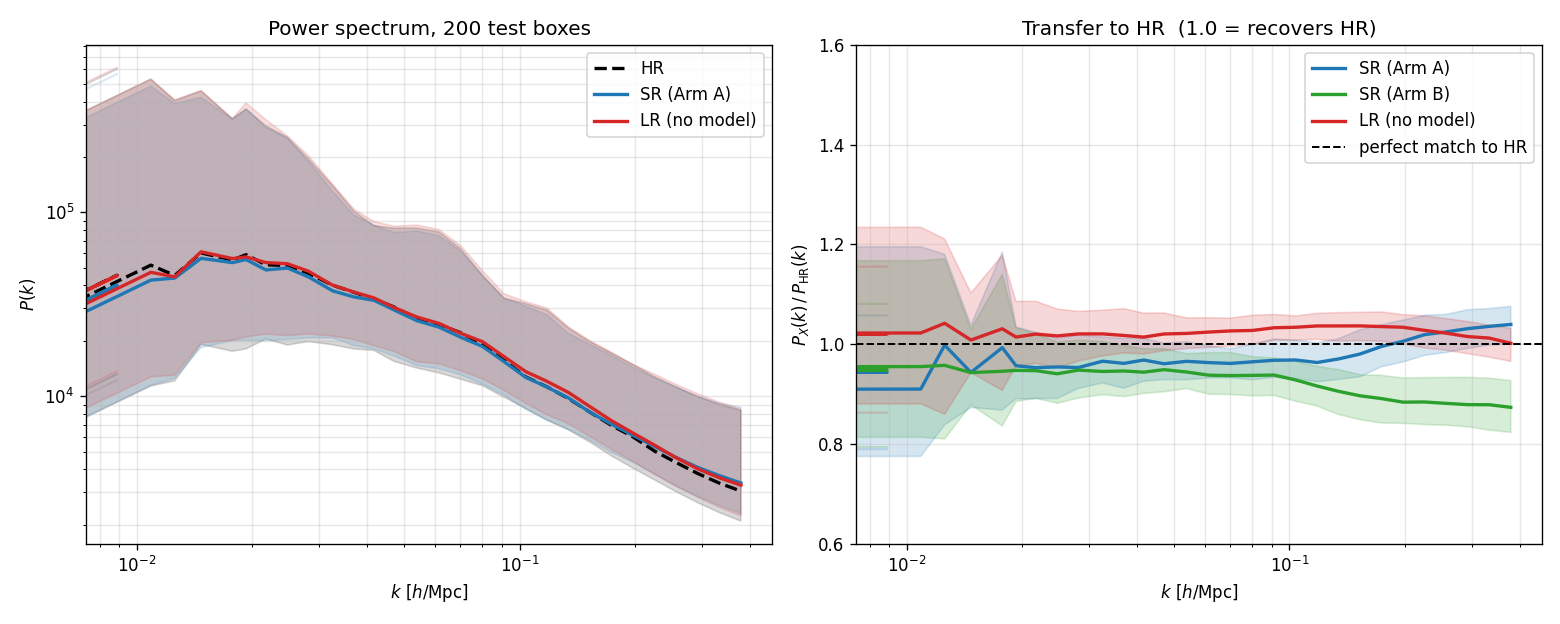
\includegraphics[width=0.98\linewidth]{figures_cmass/sr_vs_hr_pk.png}
\caption{\textbf{Left:} $P(k)$ of HR, SR (Arm A), and LR over $200$ test boxes
(median $+$ $16/84\%$ band). \textbf{Right:} transfer to HR; $1.0$ recovers HR.
SR (Arm A) sits near $1$ at all scales; Arm B's overlap blending slightly
suppresses small-scale power (transfer $0.88$).}
\label{fig:srs-srvshr}
\end{figure}

\paragraph{2. Field structure.} Beyond the power spectrum, SR keeps the field
structure of HR (Arm A, $16$ test boxes, \texttt{match\_stats\_cmassA.txt}):

\begin{table}[h]
\centering
\caption{SR vs HR field-match statistics (Arm A).}
\label{tab:srs-match}
\begin{tabular}{lll}
\toprule
quantity & value & reading \\
\midrule
total count ratio $\sum\mathrm{SR}/\sum\mathrm{HR}$ & $0.965\pm0.172$ & counts conserved on average; large per-box scatter \\
real-space std ratio & $1.008\pm0.100$ & clustering amplitude matches; not blurred \\
void fraction SR / HR ($<0.5$) & $0.855$ / $0.833$ & SR keeps voids empty, like HR \\
cross-coherence $r$, $k<0.05$ & $0.951$ & large-scale structure matches cell-by-cell \\
cross-coherence $r$, $k>0.2$ & $0.403$ & small-scale structure decorrelates \\
\bottomrule
\end{tabular}
\end{table}

\paragraph{3. Cosmology.} The cosmology comparison in the original report used
mislabeled cosmologies, an indexing bug we describe and fix in
\S\ref{sec:srs-correction}, so those numbers are not shown here. With correct
labels a single box constrains $\Omega_m$ and $\sigma_8$; at the power spectrum
level the raw LR field is already HR-like, while at the field level an SR-trained
posterior transfers to HR and an LR-trained one does not
(\S\ref{sec:srs-correction}, Table~\ref{tab:srs-corrected}).

\paragraph{4. Seam.} Neither arm introduces a stitching seam: the $x{=}64$
internal-seam excess is $\approx1$ for both
(Table~\ref{tab:srs-seam}, Fig.~\ref{fig:srs-seam}). Arm A shows a mild generic
ripple near \emph{any} boundary plane (seam-distance ratio $1.17$); Arm B's
overlap removes it ($1.00$) at a small cost in Pk RMS.

\begin{table}[h]
\centering
\caption{Seam and stitched-fidelity metrics, $200$ test boxes. ``Excess'' is
boundary error over interior error; $\approx1$ means no seam.}
\label{tab:srs-seam}
\begin{tabular}{lccp{5.2cm}}
\toprule
metric & Arm A naive & Arm B overlap & reading \\
\midrule
$x{=}64$ internal-seam excess & $0.9934$ & $0.9998$ & no internal seam either arm \\
seam-distance ratio ($d{=}0/d{\ge}8$) & $1.1729$ & $1.0032$ & generic boundary ripple, removed by overlap \\
$x{=}0$ periodic edge (control) & $0.9930$ & $0.9993$ & box edge behaves like interior \\
stitched PkRMS$_{\log_{10}}$ vs HR & $0.0637$ & $0.0678$ & stitched power-spectrum match \\
\bottomrule
\end{tabular}
\end{table}

\begin{figure}[t]
\centering
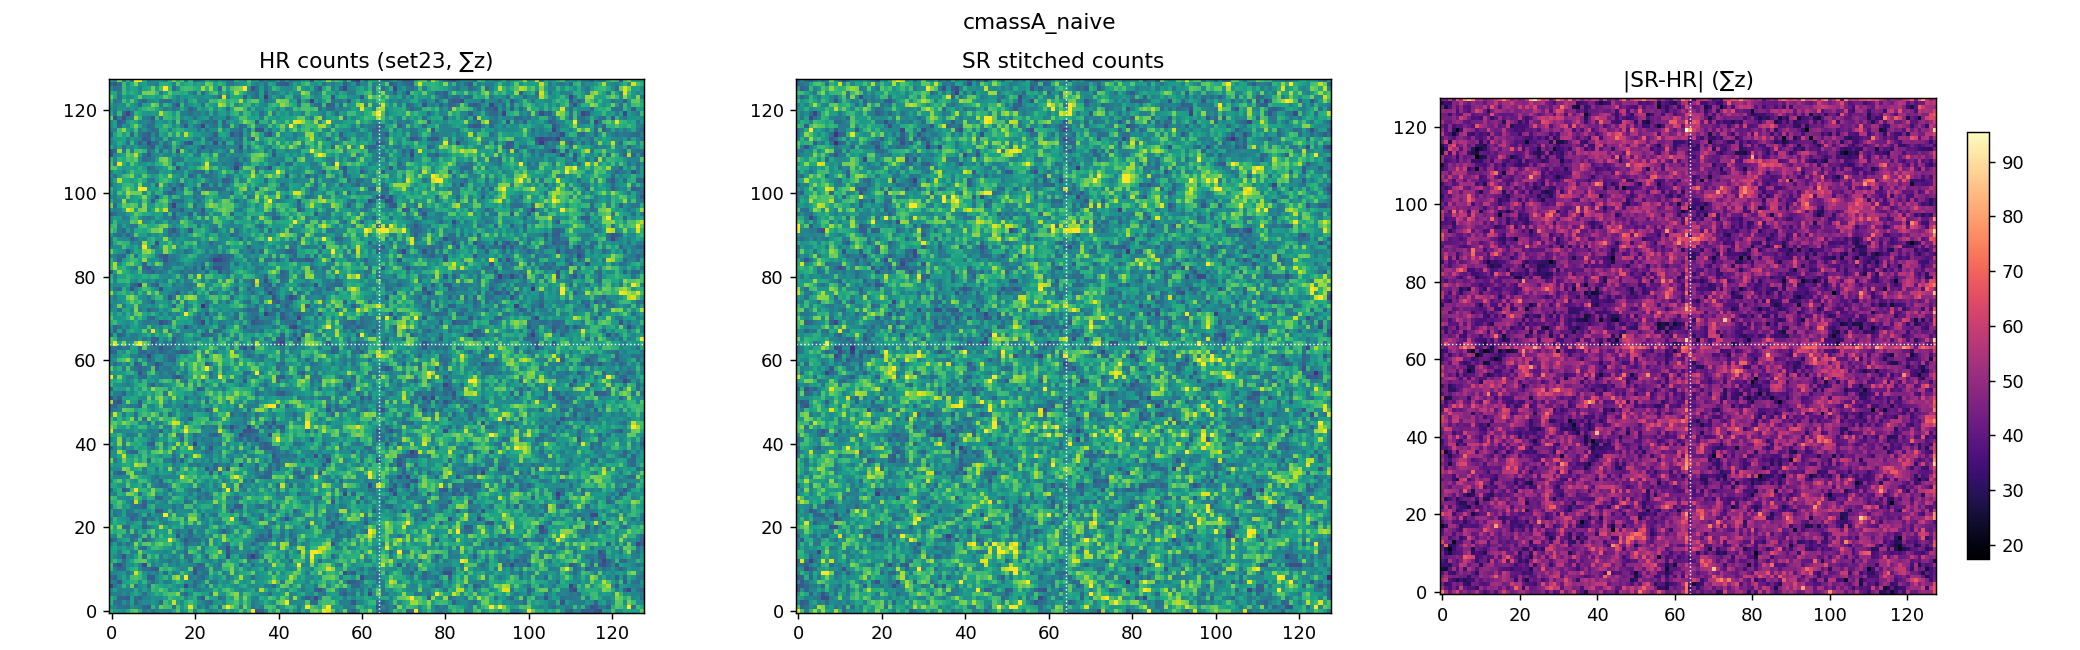
\includegraphics[width=0.95\linewidth]{figures_cmass/seam_cmassA_naive_slice.png}
\caption{Projected count maps for one test box (Arm A): HR, stitched SR, and the
absolute residual $|\mathrm{SR}-\mathrm{HR}|$. White dotted lines mark the
$x{=}64$, $y{=}64$ core boundaries; the residual shows no elevated ridge along
them.}
\label{fig:srs-seam}
\end{figure}

\paragraph{Per-scale diagnostic panels.} Figure~\ref{fig:srs-pkpanel} shows the
full-box $P(k)$, transfer, and cross-coherence for Arm A. The transfer sits near
$1$ at all scales (right amount of power); the cross-coherence is near $1$ at
large scales and falls toward small scales (structure placement is recovered at
large scales only). The per-patch panel
(\texttt{figures\_cmass/pk\_panel\_patch\_cmassAfix.png}) and the projection panels
(\texttt{projection\_box\_cmassAfix\_set23.png},
\texttt{projection\_patch\_cmassAfix\_set23\_p0.png}) tell the same story; Arm~B's
panels carry the \texttt{cmassB} suffix.

\begin{figure}[t]
\centering
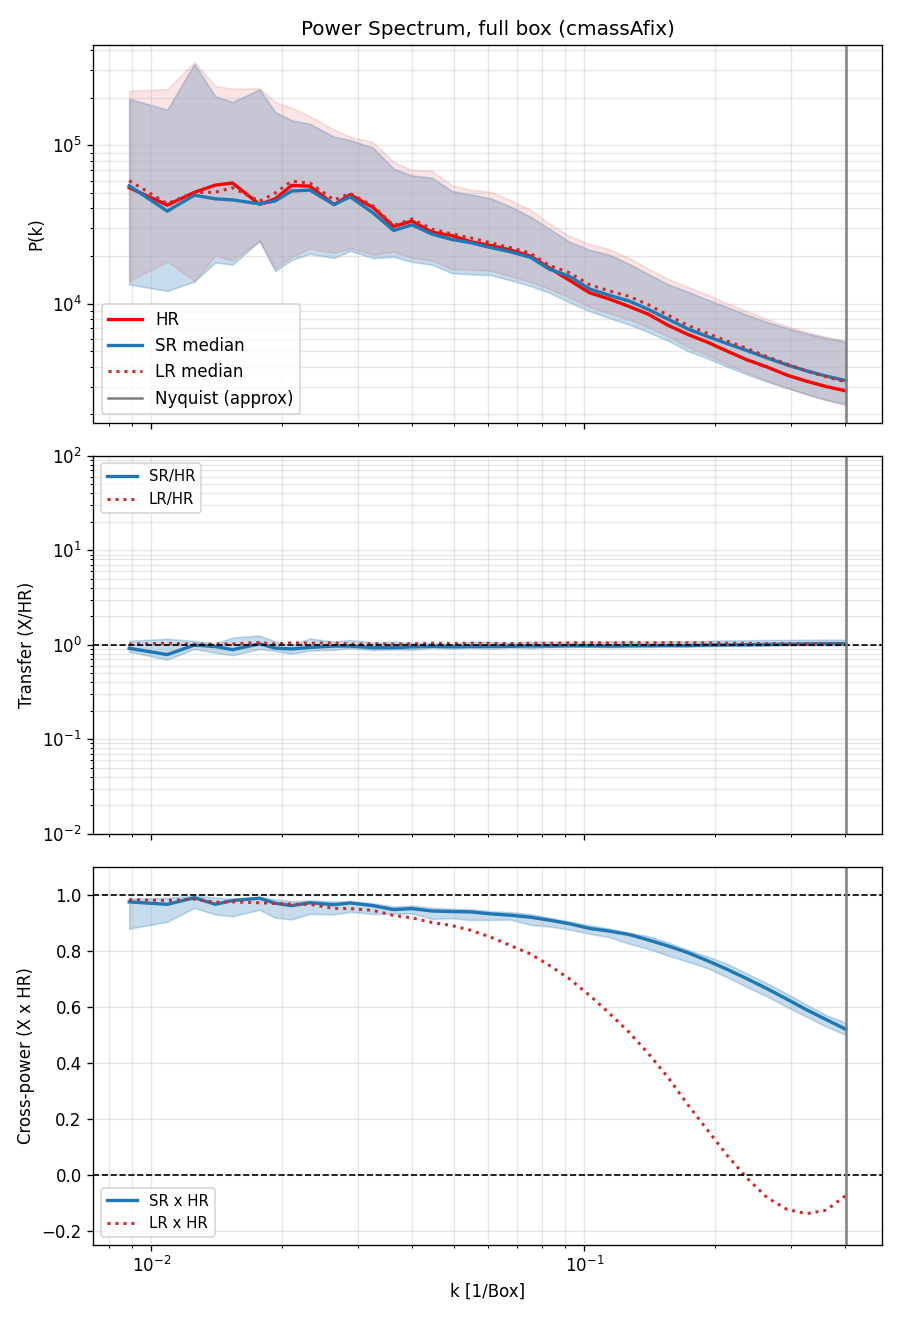
\includegraphics[width=0.5\linewidth]{figures_cmass/pk_panel_box_cmassAfix.png}
\caption{Full-box diagnostic for the conditioned generator (fiducial cosmology,
$16$ test boxes): $P(k)$ of HR (red), SR (blue median $+$ band), and LR (dotted
red); transfer $T(k)=P_X/P_\text{HR}$ on a linear axis with the 16 to 84
percentile band for both SR and LR, the legend reporting the RMS deviation of
each ratio from unity; and cross-coherence $r(k)$. The SR median transfer sits
below unity for $k<0.1$, a systematic large-scale power deficit of roughly 5 to
10 percent, while LR sits slightly above unity; SR does not tighten the transfer
scatter relative to LR. In $r(k)$, SR stays near unity to smaller scales while
LR decorrelates.}
\label{fig:srs-pkpanel}
\end{figure}

\subsection{Diagnostic: What is NOT Working}

\paragraph{Small-scale structure decorrelates, and this is fundamental.} SR
matches HR cell-by-cell at large scales ($r{=}0.95$ for $k<0.05$) but loses the
match at small scales ($r{=}0.40$ for $k>0.2$, Table~\ref{tab:srs-match}). This
is not a capacity bug: it is set by how much information the LR input carries
about HR. LR and HR share large-scale modes but the voxel-by-voxel LR$\leftrightarrow$HR
correlation is only $\approx0.06$, so the exact small-scale realization is simply
not present in the input. The model can match the small-scale \emph{statistics}
(transfer $\approx1$, real-space std ratio $1.008$) but cannot reproduce the
exact placement of individual halos. The noise injection
(Eq.~\ref{eq:srs-residual}) exists precisely because of this: it draws a
plausible small-scale field rather than regressing to a blur.

\paragraph{Per-box total-count scatter.} The total halo count is conserved on
average but with $\sim17\%$ per-box scatter ($\sum\mathrm{SR}/\sum\mathrm{HR}=
0.965\pm0.172$). A count-aware output head (predict a rate and sample Poisson
counts) would tighten this; it is the one clearly addressable imperfection. \SG{I would think this isn't necessary to fix, we don't care about the number of halos after all.}

\paragraph{Overlap suppresses small-scale power.} Arm B's overlap blending lowers
the small-scale transfer to $0.88$ (Table~\ref{tab:srs-pk}), so on the power
spectrum the naive Arm A is the better super-resolver. Overlap removes a small
generic boundary ripple but buys no fidelity, because on this continuous count
data there is no real seam to fix, the clean version of the mentor 2.1 vs 2.2
comparison.

\paragraph{Where the cosmology value is.} At the power spectrum level the raw LR
field is already close to HR, since they share large-scale modes, so the power
spectrum is a forgiving summary with little headroom. The model's value is at the
field level (variance, voids, small-scale structure), which the power spectrum
summary is insensitive to. The corrected cross-fidelity in
\S\ref{sec:srs-correction} bears this out: SR and LR are indistinguishable at the
power spectrum level, but at the field level an SR-trained posterior transfers to
HR while an LR-trained one does not.

\subsection{What I'm Trying Next}
\label{sec:srs-next}

The diagnostics above point to one limit that may be fundamental (small-scale
decorrelation) and a few that are clearly fixable (count scatter, small-scale
realism). The plan below is ordered so that we \emph{measure} the limit before
spending effort trying to beat it. None of these results are in yet; this is the
roadmap, not an experiment log.

\paragraph{Step 0, measure the information ceiling first.} Before trying to
improve the small-scale match, we need to know whether $r{=}0.40$ at small scales
(Table~\ref{tab:srs-match}) is the best any model could do from this input, or a
weakness of the current one. Two cheap diagnostics settle it:
\begin{itemize}
  \item \textbf{LR$\leftrightarrow$HR cross-coherence $r_\text{LR,HR}(k)$.} The
  cross-coherence of the \emph{raw input} against HR (no model) is the ceiling:
  no function of LR can place small-scale structure better than the input
  already correlates with HR. If $r_\text{SR,HR}(k)\approx r_\text{LR,HR}(k)$ at
  small $k$, the model is already at the ceiling and the limit is fundamental;
  if it sits well below, there is recoverable structure left on the table. (Only
  per-box $P(k)$ is currently saved, not the cross-spectrum, so this needs one
  re-run that keeps the fields.)
  \item \textbf{No-noise ablation.} Train the same generator with the noise
  injection off (a plain regressor). Theory predicts this should \emph{raise} the
  small-scale cross-coherence a little (a regressor targets the conditional mean,
  the best cell-by-cell predictor) but \emph{lower} the small-scale transfer well
  below $1$ (the conditional mean is blurry). Seeing exactly that trade-off would
  confirm that the noise/GAN is the right choice for a power-spectrum target, and
  would quantify how much cell-by-cell accuracy is being traded for correct
  statistics.
\end{itemize}

\paragraph{Step 1, fix the count scatter and small-scale realism (independent
of the ceiling).} These help regardless of what Step 0 finds:
\begin{itemize}
  \item \textbf{Count-aware (Poisson) output head.} Instead of predicting a
  count directly, predict a non-negative rate $\lambda$ per cell and sample the
  count as $n\sim\mathrm{Poisson}(\lambda)$. Halo counts are discrete and sparse,
  so a Poisson head models the small-scale graininess as actual shot noise rather
  than a smeared residual, and should tighten the $\sim17\%$ per-box total-count
  scatter (Table~\ref{tab:srs-match}), the one clearly addressable imperfection.
  \item \textbf{Explicit statistics terms in the loss.} Add a one-point PDF /
  variance matching term so small-scale sharpness is enforced directly, rather
  than relying on the adversarial term alone to find it.
  \item \textbf{Loss rebalance.} The current weights are $\lambda_\text{rec}{=}2$,
  $\lambda_\text{pk}{=}2$, $\lambda_\text{adv}{=}1$
  (Eq.~\ref{eq:srs-lossG}). The $L_1$ term blurs; lowering it and raising the
  adversarial weight should push toward correct statistics, at a known cost in
  cell-by-cell accuracy, per the same trade-off as the no-noise ablation.
\end{itemize}

\paragraph{Step 2, extract more of the available information (only if Step 0
shows headroom).} If $r_\text{SR,HR}$ sits below the LR$\leftrightarrow$HR
ceiling, the model is under-using its input. A larger receptive field, or feeding
each patch more neighbour context, would let it use more of the LR field to
predict the residual. This only helps if there is headroom to recover.

\paragraph{Step 3, raise the ceiling by changing the \emph{input}, not the
model.} The small-scale cell-by-cell limit is set by the information in the LR
input (the voxel-by-voxel LR$\leftrightarrow$HR correlation is only
$\approx0.06$). No amount of model capacity raises that; only more informative
inputs do. Candidates: feed the shared small-scale \emph{initial conditions}
(which the coarse LR count field has discarded), or add the LR velocity / particle
fields. This is the only route to a meaningful gain in small-scale cross-coherence,
and is the natural bridge to the displacement-field model of \S5, which already
carries that extra information.

\paragraph{Summary.} Steps 0--1 are the near-term plan: measure the ceiling, then
add a Poisson head and statistics losses to fix the count scatter and sharpen the
small-scale field. Steps 2--3 are contingent on what Step 0 reveals. For a
cosmology deliverable the priority is statistical fidelity (which Steps 0--1
target); exact small-scale reconstruction (Step 3) is a larger, input-level
change worth it only if cell-by-cell recovery becomes the goal.

\subsection{Follow-Up Results: New Protocol from the Mentor Meeting}
\label{sec:srs-followup}

A mentor meeting after the report above changed two things about how we train
and evaluate this model. First, the real goal is not to match HR with SR by
itself. The real goal is to train a posterior model on SR output and have it
work well when it is tested on real HR data, since HR simulations are too
expensive to train a posterior model on directly. Second, the power spectrum
term was removed from the training loss, since it was also our main success
metric and that is a weak test. This subsection reports what we found. Some of
the training runs below are still in progress at the time of writing, so
numbers marked as current are read from the latest completed epoch, not a
final result.

\paragraph{Held-out check: the bispectrum.} A fair worry is that our power
spectrum result looks good only because the power spectrum was also in the
training loss. To check this we measured the bispectrum, a higher-order
statistic that was never used anywhere in training or model selection. If SR
only matches the power spectrum and nothing else, the bispectrum should show
no improvement over the raw LR input.

\begin{figure}[t]
\centering
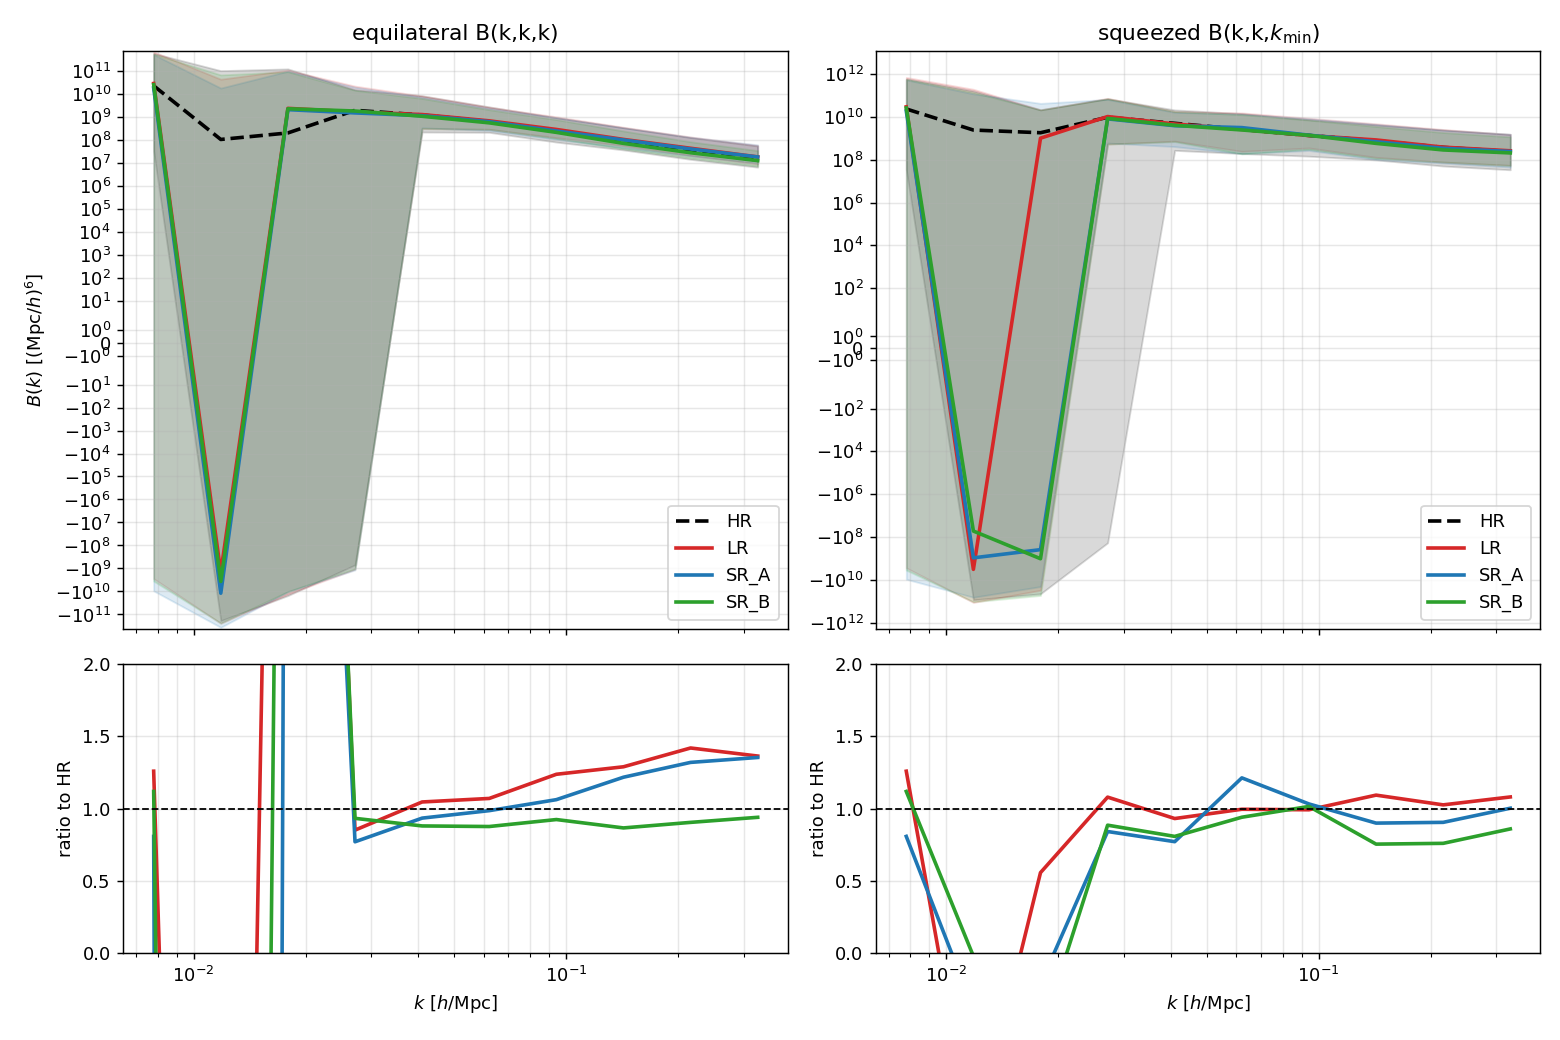
\includegraphics[width=0.95\linewidth]{figures_cmass/bispectrum_hr_lr_srA_srB.png}
\caption{Bispectrum of HR, LR, and SR (both arms), on $16$ test boxes. Top:
equilateral and squeezed bispectrum, HR in black. Bottom: ratio to HR. SR
removes most of the systematic excess that LR has at the plotted scales,
without ever training on this statistic.}
\label{fig:srs-bispec}
\end{figure}

On the equilateral configuration, LR sits about $6$ to $13$ percent above HR
across the middle range of scales. SR removes most of this gap without ever
seeing a bispectrum during training, and it does this for both arms. This is
evidence that the model is not simply fitting the training metric. It is
correcting real structure in the field that also shows up in a statistic it
never saw. (The figure uses the earlier models trained \emph{with} the power
spectrum loss; the no-Pk models of the following paragraphs preserve the
bispectrum at least as well, so removing that loss did not degrade this
held-out statistic either.)

\paragraph{Removing the power spectrum loss.} Following the meeting, we
retrained the model with the power spectrum term switched off
($\lambda_\text{pk}{=}0$ in Eq.~\ref{eq:srs-lossG}), so the loss is only the
adversarial and $L_1$ terms. We also changed which checkpoint counts as "best"
to the real-space $L_1$ error, since selecting on the power spectrum would
have been the same kind of leak we were trying to remove.

\begin{figure}[t]
\centering
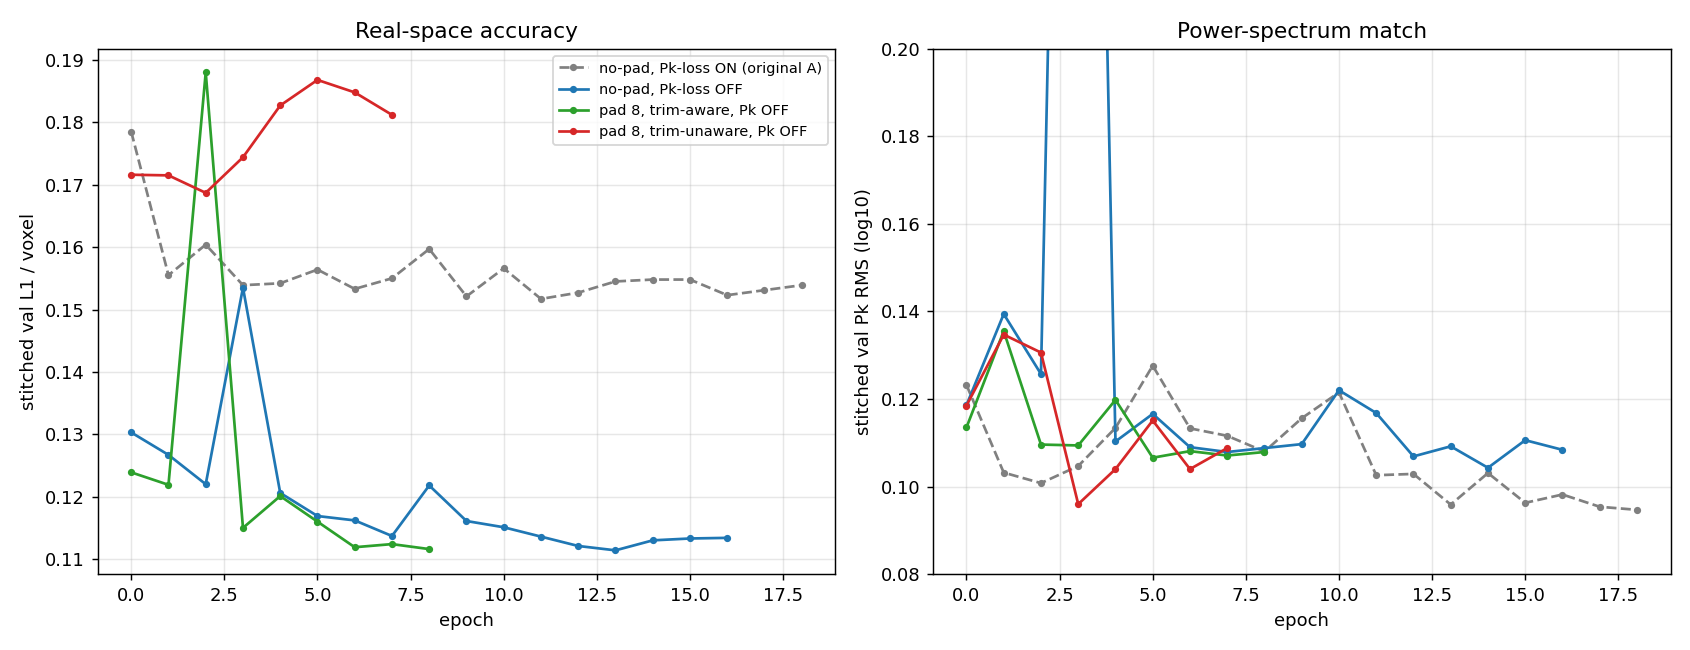
\includegraphics[width=0.98\linewidth]{figures_cmass/protocolv2_cmass.png}
\caption{Stitched validation curves under the new protocol (power spectrum
loss off). Left: real-space $L_1$ error. Right: power spectrum RMS error. Grey
dashed: the original Arm A with the power spectrum loss on, for comparison.
These runs are still training; curves stop at the most recent completed
epoch.}
\label{fig:srs-protocolv2}
\end{figure}

Two things stand out so far. First, without the power spectrum term, the
real-space $L_1$ error becomes clearly better than the original run at the
same point in training (left panel, blue and green curves sit below the grey
dashed curve). Second, the power spectrum error does get a little worse
without its loss term, but it does not collapse: it settles into roughly the
same range as before, just a bit noisier. So the power spectrum term was
buying us a small amount of power spectrum accuracy at a real cost in
real-space accuracy. It was not the only reason the power spectrum matched
well; the adversarial and reconstruction terms carry most of that on their
own.

\paragraph{Does padding help, once the power spectrum loss is out of the way?}
The report above found that padding (Arm B) did not beat no padding (Arm A) on
the power spectrum. The mentor pointed out two different ways this could
happen, and that they make different, testable predictions:
\begin{itemize}
  \item \textbf{Trim-aware.} The model is trained knowing that only the middle
  part of its output will be kept; the loss only looks at that middle part.
  This is what Arm B already did. If this is working correctly, padding should
  train at least as well as no padding, since it has strictly more context for
  the same target.
  \item \textbf{Trim-unaware.} The model is trained as if its whole padded
  output matters, including the edge region that gets thrown away later. If
  the model leans on that edge region during training, it should look fine
  during training but generalize worse once the edge is cut off at test time.
\end{itemize}
We trained both versions with the power spectrum loss off, so the comparison
is not confused by that term. Figure~\ref{fig:srs-protocolv2} shows all three
runs together (no padding, trim-aware padding, trim-unaware padding).

The trim-aware version (green) matches or beats no-padding (blue) on both
real-space error and power spectrum error at almost every epoch measured so
far. This supports the first prediction: once the model is told correctly what
part of its output is graded, more context helps rather than hurts. The
trim-unaware version (red) is clearly worse on real-space error than both
other runs, and does not close that gap as training continues. This supports
the second prediction: a model that is allowed to rely on the part of its
output that gets discarded at test time pays for that at test time. Put
together, the original result that padding did not help was most likely
caused by the power spectrum loss, not by padding itself.

We also reran the older, padding-with-power-spectrum-loss model for more
epochs to check whether it had simply not been trained long enough. Fifteen
additional epochs did not beat its early best score, so that run was not
undertrained; the training recipe, not the training time, was the limiting
factor.

\subsection{The Goal Metric: Corrected Cross-Fidelity Results}
\label{sec:srs-correction}

\paragraph{The bug.} After the analysis above, a routine physical sanity check
failed in a way that could not be real: the amplitude of the power spectrum had
essentially zero correlation with $\sigma_8$, and a fit of the power spectrum to
the five parameters explained only $0.2\%$ of the variance. The power spectrum
amplitude must scale with $\sigma_8$, so this pointed to a labeling error, not to
physics. Tracing it, we found that the processed count fields were written in
string-sorted simulation order ($0, 1, 10, 100, 1000, \dots$) while the cosmology
table is indexed numerically. Field number $k$ is therefore the halo field of
simulation string-sort$(k)$, not simulation $k$, so every field in the whole
pipeline was paired with the wrong cosmology. We proved this exactly: using the
original halo catalogs, the field halo count matches the catalog count under the
string-sort permutation for all $2000$ simulations, while the identity mapping
matches only the two fixed points. We corrected the cosmology table to field
order, backed up the old one, and patched the builder so it cannot regenerate the
wrong order.

\begin{figure}[h]
\centering
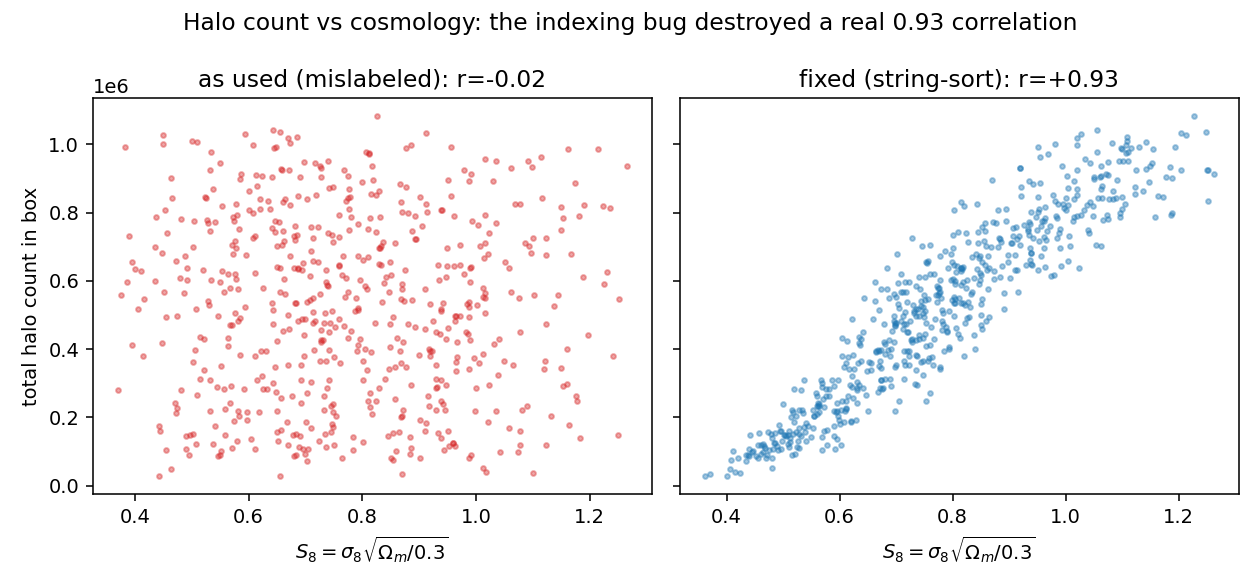
\includegraphics[width=0.85\linewidth]{figures_cmass/labelbug_count_vs_s8.png}
\caption{The indexing bug in one picture. Total halo count in a box against
$S_8 = \sigma_8\sqrt{\Omega_m/0.3}$. As the pipeline used the labels (left) the
correlation is zero; with the string-sort mapping corrected (right) the true
$0.93$ correlation reappears. Halo abundance must track $S_8$, so the left panel
was the signature of a labeling error, not of uninformative data.}
\label{fig:srs-labelbug}
\end{figure}

\paragraph{What this changes, and what it does not.} Every cosmology number we
computed before this point used the labels and is affected; the earlier
cross-fidelity tables have been removed and are replaced by the corrected results
below, and the earlier reading that the SR-versus-LR difference was an irreducible
coin flip was itself a product of the mislabeling. The results that do not use the
labels are unaffected and still stand: the power spectrum match of SR to HR, the
held-out bispectrum, the field-match statistics, the seam test, and the real space
error. The generator conditions on the cosmology as a style vector and was trained
with the scrambled labels, so its conditioning was uninformative during training;
we return to this at the end.

\paragraph{The data is informative after all.} With correct labels the picture
inverts. A halo count in this suite carries a strong cosmological signal: the
total halo count alone correlates with the combination $S_8 = \sigma_8
\sqrt{\Omega_m/0.3}$ at $0.93$ and with $\Omega_m$ at $0.85$. A Fisher forecast on
a single-box power spectrum now explains $98\%$ of the variance, where it
explained $0.2\%$ before, and it constrains $\Omega_m$ and $\sigma_8$ well, with
$\Omega_b$, $h$ and $n_s$ weak or unconstrained, which is the textbook pattern for
a low-redshift halo field. The field-level network tells the same story: after the
fix its predicted $\Omega_m$ correlates with the truth at $0.90$ on both training
and test boxes, where before the fix the correlation was zero and the output was a
constant. So the earlier conclusion that a single box carries almost no cosmology
was an artifact of the labeling, not a property of the data.

\begin{figure}[h]
\centering
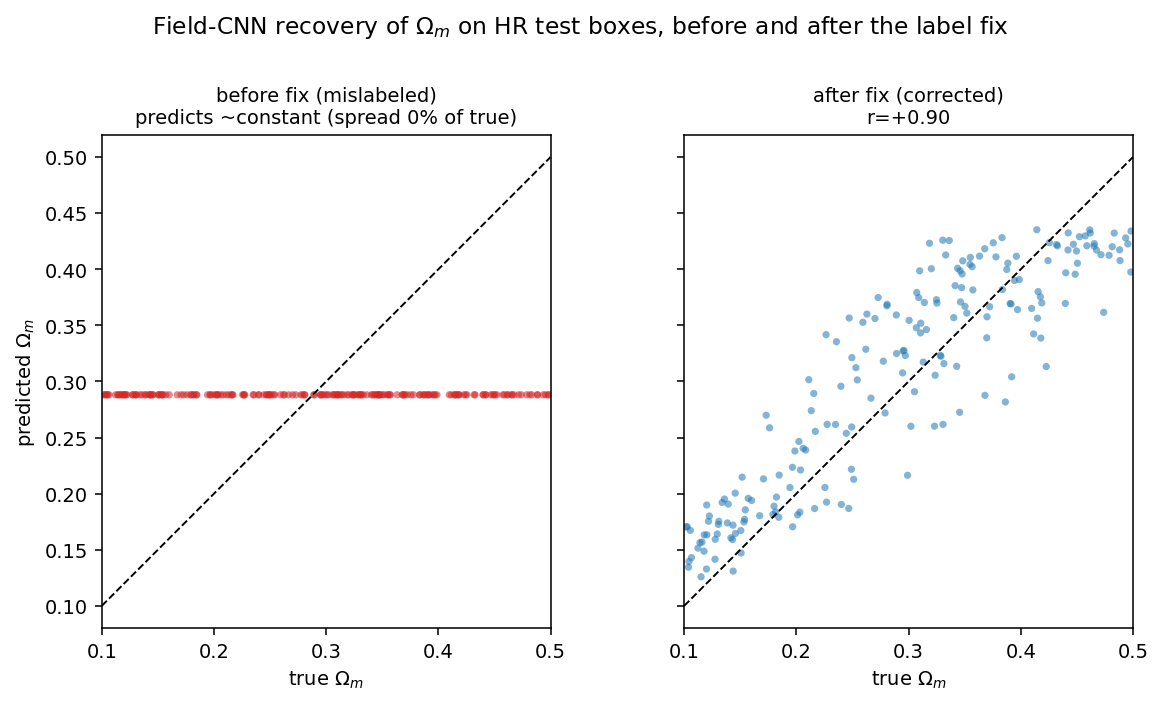
\includegraphics[width=0.82\linewidth]{figures_cmass/field_recovery_Om_cmass.png}
\caption{Field-level CNN recovery of $\Omega_m$ on HR test boxes, before and after
the label fix. Before (left) the prediction is flat and uncorrelated with the
truth (the network returns a near-constant); after (right) it tracks the diagonal
at a correlation of about $0.90$, on both training and test boxes. Same
architecture, same data, only the labels changed.}
\label{fig:srs-recovery}
\end{figure}

\begin{figure}[h]
\centering
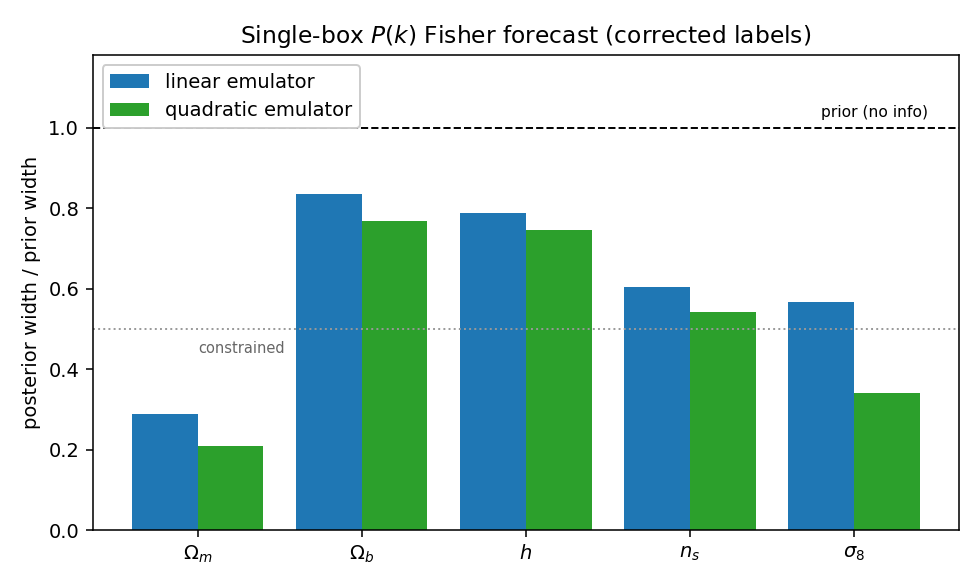
\includegraphics[width=0.72\linewidth]{figures_cmass/fisher_corrected_cmass.png}
\caption{Fisher forecast for a single-box power spectrum with corrected labels:
posterior width divided by prior width per parameter (lower means better
constrained, $1$ means no information). $\Omega_m$ is well constrained and
$\sigma_8$ is constrained, while $\Omega_b$, $h$ and $n_s$ are weak, the textbook
pattern for a low-redshift halo field. Two emulators (linear average slope and
quadratic at the prior centre) bracket the estimate.}
\label{fig:srs-fisher}
\end{figure}

\paragraph{Corrected cross-fidelity, and where SR helps.} We re-ran the goal
metric with correct labels at two levels, the power spectrum summary and the full
field. We train the posterior on one source, apply it to HR, and compare to a
posterior trained on HR, using an ensemble of independently retrained estimators
so the numbers are not single draws. Table~\ref{tab:srs-corrected} gives the
result.
\begin{table}[h]
\centering
\caption{Corrected cross-fidelity KL to HR (posterior trained on the named source,
evaluated on HR), lower is better, with the HR-to-HR floor for reference. Summary
uses the power spectrum; field uses a three-dimensional CNN posterior on the full
box.}
\label{tab:srs-corrected}
\begin{tabular}{lccc}
\toprule
level & LR (raw) & SR & HR floor \\
\midrule
summary $P(k)$ & $0.032$ & $0.088$ & $0.028$ \\
field (CNN)    & $0.49 \pm 0.81$ & $\mathbf{0.024}$ & $0.022$ \\
\bottomrule
\end{tabular}
\end{table}
\begin{figure}[h]
\centering
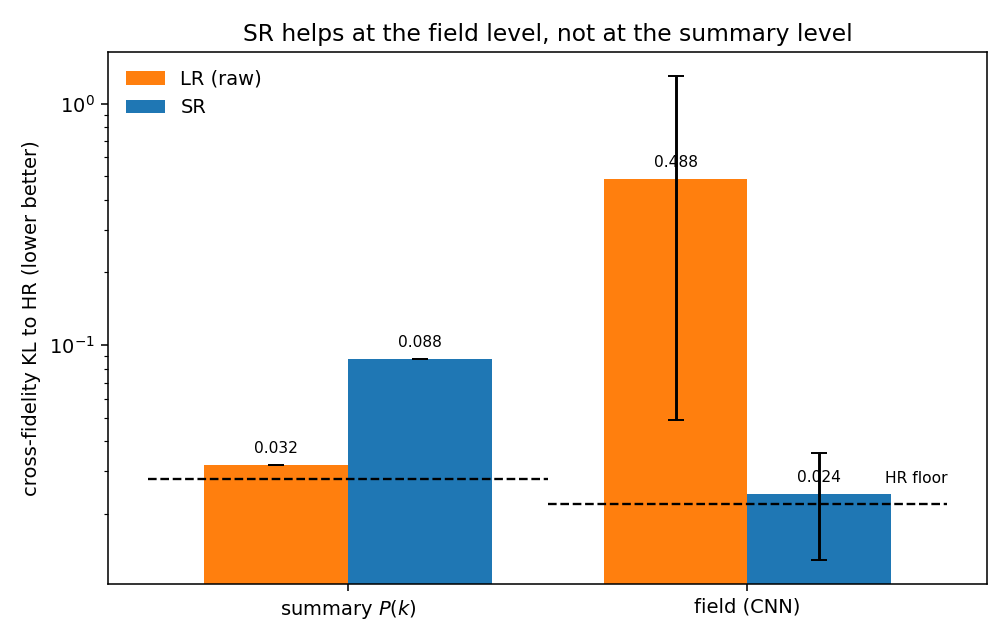
\includegraphics[width=0.7\linewidth]{figures_cmass/crossfid_corrected_cmass.png}
\caption{Corrected cross-fidelity KL to HR (log scale, lower is better) at the two
levels, with the HR-to-HR floor shown as the dashed line. At the summary level the
raw LR field is already at the floor and SR does not help. At the field level, an
LR-trained posterior does not transfer to HR (large and unstable), while an
SR-trained posterior sits at the floor. SR helps exactly where it corrects the
field.}
\label{fig:srs-crossfid-corrected}
\end{figure}
The two levels point in opposite directions, and both make sense. At the summary
level the raw LR power spectrum is already at the HR floor, so an LR-trained
posterior transfers to HR as well as an HR-trained one does, and there is no gap
for SR to close; SR even hurts a little, because the generator reshapes the
small-scale power in a way that does not match how HR responds to cosmology. At
the field level the raw LR box looks different enough from HR that an LR-trained
posterior does not transfer, and it does so unreliably, sometimes acceptably and
sometimes catastrophically, which is why its number carries such a large spread.
SR corrects the field to look like HR, so an SR-trained posterior transfers to HR
reliably, at the floor. This is exactly the deployment case the project is built
on, train the inference model on cheap SR-corrected boxes and apply it to
expensive HR, and at the field level SR makes it work where raw LR does not.

\paragraph{Padding on the goal metric.} We ran the two padding variants through
the corrected cross-fidelity at the summary level as well
(Table~\ref{tab:srs-padding}). Among the SR models the ordering from the earlier
report survives: no padding is best on the goal metric, trim-aware padding is
worse, and trim-unaware is worst, so for the cosmology objective the no-padding
model is the one to use. All three sit above the raw LR control at this level,
consistent with LR already being HR-like on the power spectrum. One number does
change under the fix: the mislabeled data made trim-unaware look catastrophic (a
factor of several hundred above the others), while with correct labels it is the
weakest variant by about a factor of two, not a blow-up. Its real-space error
(Figure~\ref{fig:srs-protocolv2}) remains the clearest and most direct sign that
it is the least reliable model.
\begin{table}[h]
\centering
\caption{Corrected cross-fidelity KL to HR at the summary (power spectrum) level
for the SR padding variants, with the LR control and the HR floor. Lower is
better. Field-level padding numbers are future work.}
\label{tab:srs-padding}
\begin{tabular}{lc}
\toprule
model & summary cross-fidelity KL \\
\midrule
SR, no padding & $\mathbf{0.087}$ \\
SR, trim-aware padding & $0.127$ \\
SR, trim-unaware padding & $0.172$ \\
\midrule
LR (control) & $0.031$ \\
HR floor & $0.028$ \\
\bottomrule
\end{tabular}
\end{table}

\paragraph{Bottom line.} With the labels fixed, the cosmology question has a
clear answer. The data constrains $\Omega_m$ and $\sigma_8$ from a single box. At
the power spectrum level the raw LR field is already HR-like, so SR is not needed
there and slightly hurts. At the field level, which is what SR actually corrects,
an SR-trained posterior transfers to HR at the floor while a raw LR one does not,
so SR provides a real and reliable cosmology benefit exactly where it operates.
Trim-unaware padding is still the weakest variant, worst on the goal metric and
on real-space error, though the label fix shrinks its apparent failure from
catastrophic to about a factor of two. Two honest caveats remain: the
field-level LR number has a wide spread and rests on a handful of retrained
networks, so the size of the gap should be firmed up with more seeds; and because
the generator was trained with the scrambled labels, its cosmology conditioning
was uninformative, so a retrain with correct conditioning may sharpen the SR
result further. Neither caveat changes the direction: with correct labels, SR
helps cosmology at the field level.

\paragraph{A data reliability note.} Partway through these runs, the shared
data storage this project reads from filled up completely, which caused a few
training jobs to fail with a file briefly appearing missing even though it was
not actually deleted. We added a retry step to the data loader and resumed
each affected run from its last saved checkpoint, so no real training progress
was lost. This is a shared infrastructure issue, not a problem with the data or
the method.

\subsection{Files}
\begin{itemize}\itemsep0pt
  \item Data and patching: \texttt{data/patch\_dataset\_cmass.py}
  (shared ops in \texttt{data/patch\_dataset\_real.py})
  \item Model: \texttt{map2map/models/styled\_srsgan.py}
  (\texttt{G\_correct}, \texttt{D\_const})
  \item Training: \texttt{train\_patch\_cmass.py};
  run script \texttt{scripts/train\_patch\_cmass.slurm}
  \item Inference and stitching: \texttt{infer\_stitch\_cmass.py}
  \item Seam eval: \texttt{analysis/eval\_seam\_cmass.py}
  \item Box / per-patch diagnostics: \texttt{analysis/diag\_cmass.py}
  \item SR-vs-HR match stats: \texttt{analysis/match\_stats\_cmass.py}
  \item SR-vs-HR power-spectrum figure: \texttt{analysis/plot\_sr\_vs\_hr.py}
  \item Bispectrum (held-out statistic): \texttt{analysis/bispectrum\_cmass.py}
  \item Training loss curves: \texttt{analysis/plot\_losses\_cmass.py}
  \item Cross-fidelity posterior evaluation: \texttt{evaluate.py} (SR-trained
  or LR-trained posterior evaluated on HR $P(k)$)
  \item Protocol-v2 (no-Pk-loss, padding-variant) training curves:
  \texttt{analysis/plot\_protocolv2\_cmass.py}
  \item Power spectrum on counts: \texttt{analysis/power\_spectrum.py}
  (estimator \texttt{counts}); differentiable training version
  \texttt{analysis/pk\_torch.py}
  \item Posterior and KL: \texttt{inference/nde.py}, \texttt{evaluate.py};
  end-to-end eval \texttt{scripts/eval\_cmass\_wrapper.slurm}
  \item Field-level posterior (three-dimensional CNN, moment-network loss):
  \texttt{models/field\_cnn.py}, \texttt{train\_field\_cnn.py};
  SR field generation \texttt{gen\_sr\_fields.py}; capacity and recovery
  diagnostics \texttt{overfit\_test.py}, \texttt{field\_diag.py}
  \item Outputs: \texttt{runs/patch\_cmass/}; figures: \texttt{figures\_cmass/}
\end{itemize}
 from main.tex, or paste inline.
% Figures referenced live in figures_cmass/ (set \graphicspath or copy them
% next to main.tex). Every number is from runs/patch_cmass/ and FINAL.md.
% =====================================================================

\section{SRS-styled-map2map-galaxy}
\label{sec:srs}

This section documents the second model in this work at the same level of
detail as \S5. Where \S5 corrects a Lagrangian \emph{displacement} field with a
point--voxel flow matcher, this model corrects an Eulerian \emph{halo count}
field with a styled GAN. The two share the same high-level goal, make a cheap
low-fidelity (LF) simulation look like an expensive high-fidelity (HF) one, 
but operate on different data and use a different architecture.

\paragraph{Goal.} Running an accurate (high-resolution) N-body simulation is
expensive; running a fast approximate one is cheap. We want a model that takes
\emph{only} the cheap LF field and produces a corrected field (we call it the
super-resolved or \textbf{SR} field) that matches the expensive HF field. At
inference the model never sees HF: the HF field is used only to train the model
and to grade it. So every result in this section answers one question: \emph{how
close is the SR field, built from LF alone, to the HF field it never saw?}

\paragraph{Terminology.} We work one cubic sub-volume at a time. We call the
$64^3$ output sub-volume a \textbf{core}, and the (possibly larger) input
sub-volume that the model reads a \textbf{patch}. When \texttt{pad}${=}0$ the
patch and the core coincide. We use \textbf{LR}/\textbf{LF} and
\textbf{HR}/\textbf{HF} interchangeably; the data here is named LR (input) and
HR (target).

\paragraph{Two arms.} We test the boundary treatment with two arms that are
identical except for one number:
\begin{itemize}
  \item \textbf{Arm A (naive, mentor 2.1):} \texttt{pad}${=}0$. Each $64^3$ core
  is corrected and placed edge-to-edge.
  \item \textbf{Arm B (overlap, mentor 2.2):} \texttt{pad}${=}8$. Each patch is
  grown to $80^3$ with real neighbour cells (periodic wrap), only the central
  $64^3$ core is kept and placed.
\end{itemize}

\subsection{Data Preprocessing}
\textit{Source: \texttt{cmass-ili}; loader \texttt{data/patch\_dataset\_cmass.py}.}

\paragraph{Input.} We have $2000$ paired simulations at redshift $z=0.5$, run
from shared initial conditions. Each pair is a low-fidelity field (LR, from the
FastPM particle-mesh code) and a high-fidelity field (HR, from a Quijote N-body
run). Both are stored as integer \textbf{halo count grids} of shape
$128\times128\times128$ on a periodic box of side $L_\text{box}=1000\
\mathrm{Mpc}/h$ (cell size $\approx 7.81\ \mathrm{Mpc}/h$). A cell value is the
number of halos whose position falls in that cell. The fields are sparse: most
cells are zero and the mean count per cell is small (the code caches one global
count scale, the mean HR count per cell measured over $50$ training sims).
Because LR and HR share initial conditions, they describe the same structure at
two fidelities. The correspondence is between the two halo catalogs \emph{as a
whole}: there is no known one-to-one matching between individual LR and HR
halos, only between the count fields they produce.

\paragraph{Cosmology labels.} Each simulation carries a style vector
$\mathbf s=(\Omega_m,\Omega_b,h,n_s,\sigma_8)\in\mathbb R^5$, parsed from that
sim's \texttt{config.yaml}.

\paragraph{Splits.} The on-disk lists give $1600$ train, $200$ validation, and
$200$ test simulations, split by simulation index.

\begin{figure}[t]
\centering
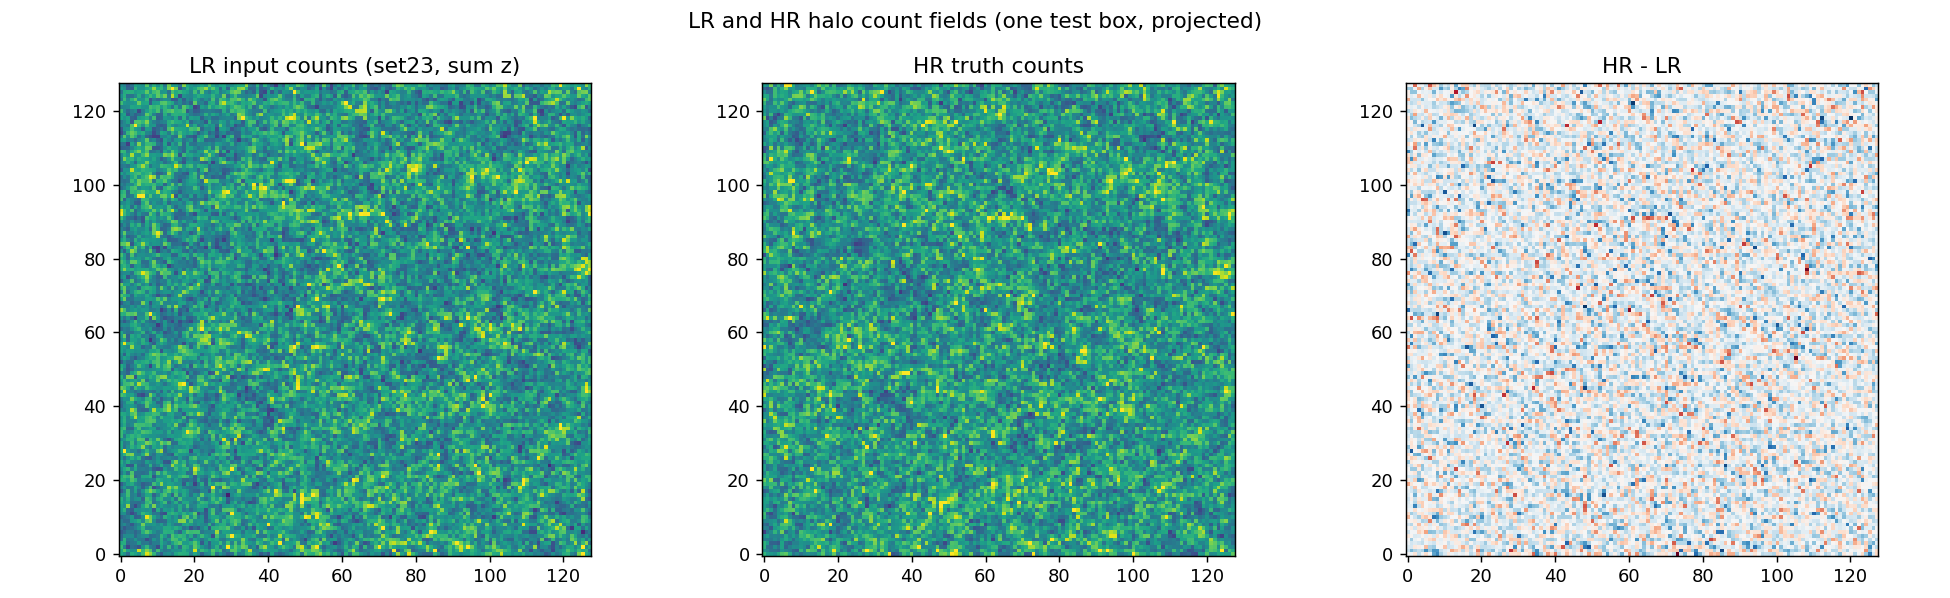
\includegraphics[width=0.9\linewidth]{figures_cmass/data_pair.png}
\caption{One LR/HR pair (projected count map). LR (FastPM, input) and HR
(Quijote N-body, target) share initial conditions and so share large-scale
structure, but differ cell-by-cell.}
\label{fig:srs-datapair}
\end{figure}

\paragraph{Model space (count transform).} The network does not learn on raw
counts; it learns in a compressed ``model space''. The default transform is
$\log(1+n)$, which tames the sparse heavy tail:
\begin{equation}
  y = \log(1+n), \qquad n = \exp(y)-1 \ \ (\text{clamped to } n\ge 0).
  \label{eq:srs-transform}
\end{equation}
Two alternative transforms exist in the code (\texttt{scale}: $n/\text{scale}$;
\texttt{delta}: model space is the overdensity itself), but all reported runs use
$\log(1+n)$. Power spectra are \emph{never} computed in model space; they are
always computed on the physical-count overdensity \SG{Is it okay if this is -1 when there are 0 halos?}
\begin{equation}
  \delta = \frac{n}{\bar n} - 1,
  \label{eq:srs-delta}
\end{equation}
with $\bar n$ the per-box mean count (the \texttt{perbox} setting used in all
runs).

\subsection{Data Pipeline (patching)}
\textit{Located in: \texttt{data/patch\_dataset\_cmass.py},
\texttt{data/patch\_dataset\_real.py} (shared patch ops).}

A model never sees the whole $128^3$ box at once. We cut the box into a
$2\times2\times2$ grid of $64^3$ \textbf{cores} (Table~\ref{tab:srs-notation}).
The cores tile the box exactly (stride $64$), so they reconstruct the box
bit-for-bit with no gaps and no double counting, the dataset's self-test
asserts this. Each model \emph{input} is a core grown by \texttt{pad} voxels on
every side, taken from the true neighbour cells with periodic wrap at the box
edge (\texttt{extract\_patch} uses \texttt{numpy.take(\dots, mode="wrap")}). So
with \texttt{pad}${=}8$ the input is $80^3$ and neighbouring patches overlap by
$2\cdot\texttt{pad}=16$ voxels; the HR \emph{target} is always the bare $64^3$
core. Because each simulation is one continuous periodic box that we crop
ourselves, the patches are real neighbours by construction, there is no data
seam (unlike the Lagrangian patches of \S5). \SG{Isn't the patch construction same in both?}

\begin{table}[t]
\centering
\caption{Notation for the CMASS count-field pipeline.}
\label{tab:srs-notation}
\begin{tabular}{llp{7.2cm}}
\toprule
Symbol & Value & Meaning \\
\midrule
$N_\text{full}$    & $128$ & full box side (voxels) \\
$P$ (\texttt{PATCH}) & $64$ & core side (voxels) \\
$N_\text{patches}$ & $8$ & cores per box ($2{\times}2{\times}2$) \\
\texttt{pad}       & $0$ (Arm A) / $8$ (Arm B) & halo width added to each face by periodic wrap \\
$L_\text{box}$     & $1000\ \mathrm{Mpc}/h$ & box side \\
$\mathbf s$        & $\in\mathbb R^5$ & cosmology vector $(\Omega_m,\Omega_b,h,n_s,\sigma_8)$ \\
$\bar n$           & per-box mean & mean count used to form $\delta=n/\bar n-1$ \\
\bottomrule
\end{tabular}
\end{table}

\begin{figure}[t]
\centering
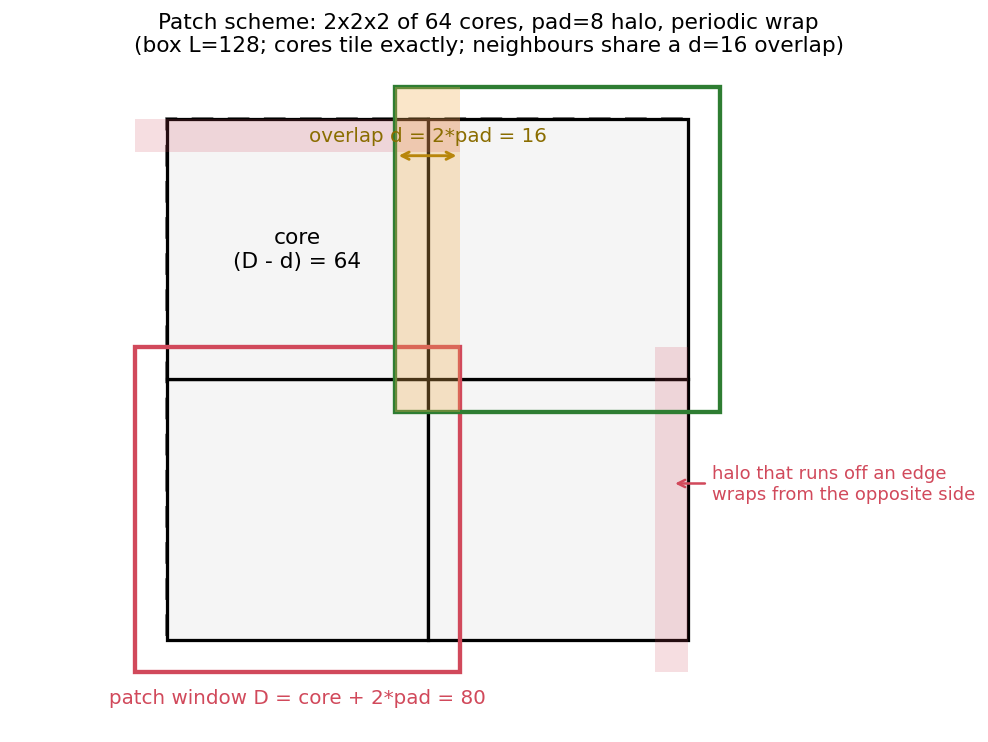
\includegraphics[width=0.82\linewidth]{figures_cmass/pipeline_patching.png}
\caption{Patch scheme. The box is cut into a $2{\times}2{\times}2$ grid of
$64^3$ cores that tile it exactly. With \texttt{pad}${>}0$ each patch is grown by
a halo of real neighbour cells (periodic wrap); only the central core is kept
and placed back.}
\label{fig:srs-patching}
\end{figure}

\paragraph{Per-simulation item.} Indexed by simulation, the dataset returns, for
all $8$ cores at once: the LR patches \texttt{lr\_in} of shape
$(8,\,1,\,64{+}2\,\texttt{pad},\,\cdot,\,\cdot)$ in model space, the HR cores
\texttt{hr\_tgt} of shape $(8,\,1,\,64,\,64,\,64)$, the style $\mathbf s$, and
the simulation index. The trainer flattens the $8$-core axis into the batch.

\begin{algorithm}[H]
\caption{\textsc{ExtractPatches} (one simulation)}
\label{alg:srs-extract}
\begin{algorithmic}[1]
\Require LR box $\mathbf L\in\mathbb R^{1\times128^3}$, HR box $\mathbf H$, \texttt{pad}
\State map $\mathbf L,\mathbf H$ to model space via Eq.~\ref{eq:srs-transform}
\For{$p=0,\dots,7$}
  \State $(i,j,k)\gets\textsc{unravel}(p,(2,2,2))$ \Comment{core origin $(64i,64j,64k)$}
  \State $\mathbf L_p\gets$ core $p$ grown by \texttt{pad} on each face, periodic wrap \Comment{$(64{+}2\,\texttt{pad})^3$}
  \State $\mathbf H_p\gets$ bare core $p$ \Comment{$64^3$}
\EndFor
\State \Return $\{(\mathbf L_p,\mathbf H_p)\}_{p=0}^{7}$, style $\mathbf s$
\end{algorithmic}
\end{algorithm}

\subsection{Model: Input/Output Specification}
\textit{Implementation: \texttt{map2map/models/styled\_srsgan.py}
(\texttt{G\_correct}, \texttt{D\_const}).}

\paragraph{What the generator computes.} The generator is a
\textbf{same-resolution residual} network: it does not change the grid size, and
it predicts a correction that is \emph{added} to the input. In model space,
\begin{equation}
  \mathrm{SR} \;=\; \mathrm{LR} \;+\; G(\mathrm{LR},\,\mathbf s,\,\mathbf z),
  \label{eq:srs-residual}
\end{equation}
where $\mathbf s$ is the cosmology vector and $\mathbf z$ is an injected noise
field (see below). Inputs and outputs are listed in
Table~\ref{tab:srs-model-io}; the generator is run once per core (the $8$ cores
of a box form a batch).

\begin{table}[t]
\centering
\caption{Tensors consumed/produced by the generator \texttt{G\_correct} for one
core (batch dimension omitted). Here $D=64{+}2\,\texttt{pad}$.}
\label{tab:srs-model-io}
\begin{tabular}{lll}
\toprule
Symbol & Shape & Meaning \\
\midrule
$\mathbf x$ (\texttt{x})       & $(1,D,D,D)$ & LR patch, model space (input) \\
$\mathbf s$ (\texttt{style})   & $(5,)$      & cosmology vector \\
$\mathbf z$ (\texttt{noise\_list}) & $2\cdot\texttt{num\_blocks}$ cubes $(1,D,D,D)$ & injected noise; fixed at inference, random in training \\
$G(\cdot)$                     & $(1,D,D,D)$ & predicted residual $\delta$ (added to $\mathbf x$) \\
\bottomrule
\end{tabular}
\end{table}

\paragraph{Internal composition.} $G$ is a constant-resolution StyleGAN2-style
network (no up/down-sampling), built from:
\begin{enumerate}
  \item \texttt{block0}: a $1{\times}1{\times}1$ style-modulated convolution
  (\texttt{ConvStyled3d}) lifting the $1$-channel input to $c_0$ channels,
  followed by a leaky ReLU.
  \item \texttt{num\_blocks} ($=4$) constant-resolution H-blocks
  (\texttt{HBlock\_const}). Each block, in order: inject noise $\to$
  $3{\times}3{\times}3$ \texttt{ConvStyled3d} (periodic ``circular'' padding)
  $\to$ leaky ReLU $\to$ inject noise $\to$ $3{\times}3{\times}3$
  \texttt{ConvStyled3d} $\to$ leaky ReLU $\to$ a $1{\times}1{\times}1$ projection
  to the output channel, accumulated into a running output $y$. The final return
  is $\mathbf x + y$ (Eq.~\ref{eq:srs-residual}).
\end{enumerate}
The channel widths come from \texttt{chan\_base} ($=128$) halved per block and
clamped to $[64,512]$. Two mechanisms make the convolutions depend on side
information:
\begin{itemize}
  \item \textbf{Style modulation.} \texttt{ConvStyled3d} is the StyleGAN2
  modulated/demodulated convolution: the cosmology vector $\mathbf s$ scales the
  convolution weights, so the same network behaves differently for different
  cosmologies. This is the only path by which $\mathbf s$ enters.
  \item \textbf{Noise injection.} Each \texttt{ConvStyled3d} is preceded by a
  per-channel learned-standard-deviation noise add (\texttt{\_NoiseInject}). At
  training time the noise is fresh Gaussian each call; at inference a
  \emph{fixed} list of noise cubes (seeded, built by \texttt{build\_noise\_list})
  is reused so outputs are reproducible. The noise is what lets the model produce
  a plausible small-scale field rather than a single blurred guess.
\end{itemize}

\paragraph{Discriminator.} \texttt{D\_const} is a constant-input-resolution
critic conditioned on the same style $\mathbf s$. It runs a head
\texttt{ConvStyled3d} then \texttt{num\_blocks} strided down-blocks (each a
periodic $3{\times}3{\times}3$ \texttt{ConvStyled3d} $+$ leaky ReLU $+$
$2{\times}$ average pool), a $1{\times}1{\times}1$ tail, and a final
$1{\times}1{\times}1$ projection to one channel, averaged over space to a single
logit per core.

\subsection{Training Step}
\textit{Located in: \texttt{train\_patch\_cmass.py}.}

The generator is trained per core (stitching is \emph{not} part of the
gradient). The total generator loss is a weighted sum of three terms,
\begin{equation}
  \mathcal L_G \;=\; \lambda_\text{adv}\,\mathcal L_\text{adv}
                  + \lambda_\text{rec}\,\mathcal L_\text{rec}
                  + \lambda_\text{pk}\,\mathcal L_\text{pk},
  \label{eq:srs-lossG}
\end{equation}
with (defaults from the original run script; see the protocol update below for
the values now in use):
\begin{itemize}
  \item \textbf{Reconstruction} $\mathcal L_\text{rec}=\lVert \mathrm{SR}-\mathrm{HR}\rVert_1$,
  a plain $L_1$ in model space (optionally Gaussian-smoothed; smoothing off in
  all runs).
  \item \textbf{Power-spectrum} $\mathcal L_\text{pk}$, the mean-squared error
  between the $\log_{10}$ power spectra of SR and HR, computed on the
  \emph{physical-count overdensity} of the $64^3$ core (Eqs.~\ref{eq:srs-transform}--\ref{eq:srs-delta}),
  Hann-windowed, with the HR side detached:
  \begin{equation}
    \mathcal L_\text{pk} = \frac{1}{|K|}\sum_{k\in K}
      \big(\log_{10} P_\text{SR}(k) - \log_{10} P_\text{HR}(k)\big)^2 .
    \label{eq:srs-pkloss}
  \end{equation}
  \item \textbf{Adversarial} $\mathcal L_\text{adv}=\mathrm{softplus}\!\big({-}D(\mathrm{SR},\mathbf s)\big)$,
  the non-saturating GAN generator loss.
\end{itemize}

\paragraph{Protocol update: what region the reconstruction and adversarial
terms see.} A \texttt{--pad-loss} setting controls how much of the generator's
output the $L_1$ and adversarial terms are computed on, independent of
\texttt{pad} itself:
\begin{itemize}
  \item \texttt{crop} (trim-aware, the setting used for Arm B above): the loss
  is computed only on \textsc{cropInterior}$(G(\mathbf x,\mathbf s),\,\texttt{pad})$,
  the $64^3$ core that is actually kept at inference time, against the bare
  $64^3$ HR core. The model is trained on exactly the region it will be graded
  on.
  \item \texttt{full}: the loss is computed on the whole $(64{+}2\,\texttt{pad})^3$
  output, against a correspondingly padded HR target (the dataset's
  \texttt{pad\_target} option). The model is trained as if the halo region it
  will later be trimmed off also mattered.
\end{itemize}
Concretely, let $\texttt{loss\_crop}=\texttt{pad}$ under \texttt{crop} and $0$
under \texttt{full}; every place above that writes $\mathrm{SR}$ means
$\textsc{cropInterior}(G(\mathbf x,\mathbf s),\,\texttt{loss\_crop})$, and the
Hann window and $P(k)$ estimator in $\mathcal L_\text{pk}$ are sized to match.
This is a controlled test of two ways padding could fail to help: see the
protocol-update subsection below for the result.

The discriminator is trained with the non-saturating GAN loss plus a lazy $R_1$
gradient penalty applied every \texttt{r1\_every} steps:
\begin{equation}
  \mathcal L_D = \mathrm{softplus}\!\big({-}D(\mathrm{HR})\big)
               + \mathrm{softplus}\!\big(D(\mathrm{SR})\big)
               + \tfrac{1}{2}\lambda_{R_1}\,\mathbb E\big\lVert \nabla_{\!x} D(x,\mathbf s)\big\rVert^2 .
  \label{eq:srs-lossD}
\end{equation}

\begin{algorithm}[H]
\caption{CMASS patch-GAN training step (one batch of cores)}
\label{alg:srs-train}
\begin{algorithmic}[1]
\Require LR patches $\mathbf x$, HR targets $\mathbf h$ (padded iff \texttt{pad-loss=full}),
         style $\mathbf s$, \texttt{pad}, \texttt{loss\_crop} ($=\texttt{pad}$ if \texttt{crop} else $0$),
         weights $\lambda_\text{adv},\lambda_\text{rec},\lambda_\text{pk},\lambda_{R_1}$
\Statex \textbf{// Discriminator}
\State $\hat{\mathbf h}\gets \textsc{cropInterior}\big(G(\mathbf x,\mathbf s),\,\texttt{loss\_crop}\big)$ \Comment{no grad}
\State $\mathcal L_D \gets \mathrm{softplus}({-}D(\mathbf h,\mathbf s)) + \mathrm{softplus}(D(\hat{\mathbf h},\mathbf s))$
\If{step $\bmod\ \texttt{r1\_every} = 0$} $\mathcal L_D \mathrel{+}= \tfrac12\lambda_{R_1}\texttt{r1\_every}\cdot R_1(D,\mathbf h,\mathbf s)$ \EndIf
\State update $D$ (Adam, grad-clip)
\Statex \textbf{// Generator}
\State $\hat{\mathbf h}\gets \textsc{cropInterior}\big(G(\mathbf x,\mathbf s),\,\texttt{loss\_crop}\big)$
\State $\mathcal L_\text{adv}\gets \mathrm{softplus}({-}D(\hat{\mathbf h},\mathbf s))$
\State $\mathcal L_\text{rec}\gets \lVert \hat{\mathbf h}-\mathbf h\rVert_1$
\State $\mathcal L_\text{pk}\gets$ Eq.~\ref{eq:srs-pkloss} on Hann-windowed overdensity of $\hat{\mathbf h}$, $\mathbf h$
       (skip if $\lambda_\text{pk}{=}0$)
\State $\mathcal L_G \gets \lambda_\text{adv}\mathcal L_\text{adv}+\lambda_\text{rec}\mathcal L_\text{rec}+\lambda_\text{pk}\mathcal L_\text{pk}$
\State update $G$ (Adam, grad-clip)
\end{algorithmic}
\end{algorithm}

\paragraph{Validation and checkpoint selection.} After each epoch we stitch the
full $128^3$ SR box for up to $40$ validation sims and report the stitched
$L_1$/voxel and the stitched-$128$ power-spectrum RMS against HR
(\S\ref{sec:srs-eval}, Eq.~\ref{eq:srs-pkrms}). A \texttt{--select} setting
chooses which of the two the saved \texttt{best.pt} tracks: \texttt{pk} (the
original setting, lowest stitched validation Pk RMS) or \texttt{l1} (lowest
stitched validation $L_1$/voxel). Selection is always on the stitched full box,
not the per-core training loss. Runs that also train with $\lambda_\text{pk}{=}0$
use \texttt{--select l1}, since selecting on Pk RMS while not training on it
would reintroduce the same metric leak in a different place.

\subsection{Inference}
\textit{Located in: \texttt{infer\_stitch\_cmass.py}.}

For one simulation: load the LR $128^3$ count box, map it to model space, run $G$
on each of the $8$ cores (with the periodic-wrap halo in Arm B), crop the halo,
stitch the cores into a $128^3$ model-space box, invert the transform to physical
counts, and clamp. \SG{are all outputs later mapped to integers, or are we fine with non-integer number of halos?} The injected noise list is fixed (seeded) so the output is
reproducible.

\begin{algorithm}[H]
\caption{CMASS inference + stitch (one simulation)}
\label{alg:srs-infer}
\begin{algorithmic}[1]
\Require LR box $\mathbf L$, style $\mathbf s$, trained $G$, mode (naive/overlap), fixed noise $\mathbf z$
\State $\texttt{pad}\gets 0$ if naive else value from checkpoint ($8$)
\State map $\mathbf L$ to model space (Eq.~\ref{eq:srs-transform})
\For{$p=0,\dots,7$}
  \State $\mathbf x_p\gets$ patch $p$ (core grown by \texttt{pad}, periodic wrap)
  \State $\mathbf c_p\gets \textsc{cropInterior}\big(G(\mathbf x_p,\mathbf s,\mathbf z),\,\texttt{pad}\big)$ \Comment{$64^3$ core, model space}
\EndFor
\State $\mathbf S\gets \textsc{stitch}(\{\mathbf c_p\})$ \Comment{$128^3$, model space}
\State $\mathbf S\gets \exp(\mathbf S)-1$, clamp to $[0,\,C_\text{max}{=}200]$, replace NaN/Inf \Comment{physical counts}
\State \Return $\mathbf S$
\end{algorithmic}
\end{algorithm}

\subsection{Crop Stitching}

Stitching is \textbf{direct placement with no averaging}. Adjacent cores tile the
box exactly (stride $64$, no overlap between cores once the halo is dropped), so
each core's $64^3$ output is written straight into its slot. In Arm B the $80^3$
patch is corrected and only its central $64^3$ core is kept; the overlap halo is
context for the convolution, never written to the output.

\begin{algorithm}[H]
\caption{\textsc{Stitch} ($8$ cores $\to$ $128^3$)}
\label{alg:srs-stitch}
\begin{algorithmic}[1]
\Require cores $\{\mathbf c_p\}_{p=0}^{7}$, each $1\times64^3$
\State $\mathbf S\gets \mathbf 0\in\mathbb R^{1\times128^3}$
\For{$p=0,\dots,7$}
  \State $(i,j,k)\gets\textsc{unravel}(p,(2,2,2))$
  \State $\mathbf S[:,\,64i{:}64i{+}64,\,64j{:}\cdots,\,64k{:}\cdots]\gets \mathbf c_p$ \Comment{direct assignment}
\EndFor
\State \Return $\mathbf S$
\end{algorithmic}
\end{algorithm}

\subsection{Evaluation}
\label{sec:srs-eval}
\textit{Located in: \texttt{analysis/eval\_seam\_cmass.py},
\texttt{analysis/diag\_cmass.py}, \texttt{analysis/match\_stats\_cmass.py},
\texttt{analysis/power\_spectrum.py}, \texttt{inference/nde.py},
\texttt{evaluate.py}.}

We evaluate the SR field against HR at three levels: a seam check (does stitching
leave a join?), field statistics (does SR have the right structure?), and
cosmology (does SR give the same parameter posterior as HR?).

\paragraph{Power-spectrum summaries.} On the count overdensity (Eq.~\ref{eq:srs-delta})
we report the power spectrum $P(k)$, the transfer ratio, and the cross-coherence:
\begin{equation}
  T(k) = \frac{P_\text{SR}(k)}{P_\text{HR}(k)},
  \qquad
  r(k) = \frac{P_{\text{SR},\text{HR}}(k)}{\sqrt{P_\text{SR}(k)\,P_\text{HR}(k)}} .
  \label{eq:srs-Tr}
\end{equation}
$T(k)=1$ means SR has the right \emph{amount} of power at scale $k$ (amplitude);
$r(k)=1$ means SR has the structure in the right \emph{place} (phase). The
scalar power-spectrum error used for checkpoint selection and seam reporting is
the log-RMS over the resolved $k$-bins:
\begin{equation}
  \mathrm{PkRMS}_{\log_{10}} = \sqrt{\frac{1}{|K|}\sum_{k\in K}
    \big(\log_{10} P_\text{SR}(k) - \log_{10} P_\text{HR}(k)\big)^2 } .
  \label{eq:srs-pkrms}
\end{equation}

\paragraph{Seam diagnostic.} \texttt{eval\_seam\_cmass.py} bins the per-cell
count error $|{\mathrm{SR}-\mathrm{HR}}|$ by distance to the nearest core face
and forms a per-position error profile along each axis. The headline number is
the \textbf{$x{=}64$ internal-seam excess}: the error on the internal core
boundary plane divided by the interior error. A value near $1$ means stitching
leaves no seam. The box edge $x{=}0$ is a periodic-boundary control.

\paragraph{Field-match statistics.} \texttt{match\_stats\_cmass.py} reports, over
$16$ test boxes: the total-count ratio $\sum\mathrm{SR}/\sum\mathrm{HR}$, the
void fraction (cells $<0.5$), the real-space cell standard-deviation ratio
$\mathrm{std}(\mathrm{SR})/\mathrm{std}(\mathrm{HR})$ (a blur check), and the
cross-coherence $r(k)$ at large ($k<0.05$) and small ($k>0.2$) scales.

\paragraph{Cosmology (posterior consistency).} This is the strongest ``does SR
match HR'' test. We voxel-count $\to$ overdensity $\to$ $P(k)$ for every box, then
train a neural density estimator $q(\theta\mid P(k))$ on the training split using
\texttt{sbi} (\texttt{SNPE\_C} with a neural-spline-flow density estimator,
\texttt{inference/nde.py}); the summary is $\log_{10}P(k)$. We train one estimator
on HR ($q_\text{HR}$) and one on each SR arm ($q_\text{SR}$). For each test box we
draw $2000$ posterior samples from each, fit a Gaussian per parameter, and report
the per-parameter Gaussian KL (\texttt{evaluate.py}):
\begin{equation}
  \mathrm{KL}\big(\mathcal N(\mu_\text{HR},\sigma_\text{HR})\,\Vert\,\mathcal N(\mu_\text{SR},\sigma_\text{SR})\big)
  = \tfrac12\!\left[\log\frac{\sigma_\text{SR}^2}{\sigma_\text{HR}^2}
    + \frac{\sigma_\text{HR}^2+(\mu_\text{HR}-\mu_\text{SR})^2}{\sigma_\text{SR}^2} - 1\right].
  \label{eq:srs-kl}
\end{equation}
$\mathrm{KL}=0$ means SR gives the identical cosmology posterior to HR. The raw LR
field (no model), pushed through the same pipeline, is the control SR must beat.

We report this comparison in two forms, and it matters which is which:
\begin{itemize}
  \item \textbf{Cross-fidelity (primary).} $q_\text{SR}$ is trained on SR power
  spectra but \emph{evaluated on the HR} $P(k)$ of each test simulation, and
  compared to $q_\text{HR}$ evaluated on the same HR $P(k)$. This is the
  deployment scenario the project targets: HR simulations are too expensive to
  train an inference model on, so the inference model is trained on cheap SR
  output and must still work when applied to (HR-like) reality. The comparison
  against an LR-trained estimator on the same HR data measures whether sampling
  in HR space (SR) survives the distribution shift better than staying in LR
  space. This metric never appears in the training loss.
  \item \textbf{Own-data (secondary).} $q_\text{SR}$ trained and evaluated on SR
  vs $q_\text{HR}$ trained and evaluated on HR, each pipeline end-to-end on
  its own field type.
\end{itemize}

\subsection{Best-Run Configuration}
\textit{Run script: \texttt{scripts/train\_patch\_cmass.slurm}; checkpoints
\texttt{checkpoints/patch\_cmass\_\{A,B\}/best.pt}.}

Both arms use the identical configuration below; they differ only in \texttt{pad}
($0$ for Arm~A, $8$ for Arm~B). This is the configuration behind every number
in \S\ref{sec:srs-results}--\S\ref{sec:srs-next}.

\begin{lstlisting}[language=bash]
--transform log1p   --nbar perbox        # log(1+n) model space; per-box nbar
--epochs 30         --sims-per-batch 1    # patch-batch = 8 cores per step
--chan-base-g 128   --chan-base-d 64  --num-blocks 4
--lambda-adv 1.0    --lambda-rec 2.0  --lambda-pk 2.0   # generator weights
--lambda-r1 10.0    --r1-every 16                       # lazy R1
--lr-g 1e-4 --lr-d 1e-4  --beta1 0.0 --beta2 0.99       # Adam
--grad-clip 1.0     --val-max-sims 40    --select pk    # select on Pk RMS
\end{lstlisting}

The best checkpoint per arm is the one with the lowest stitched validation Pk RMS
(Eq.~\ref{eq:srs-pkrms}):

\begin{center}
\begin{tabular}{lc}
\toprule
arm & best stitched val PkRMS$_{\log_{10}}$ \\
\midrule
Arm A, naive (pad $0$)  & $0.0947$ \\
Arm B, overlap (pad $8$) & $0.0963$ \\
\bottomrule
\end{tabular}
\end{center}

\paragraph{Protocol update.} Following the mentor meeting reported in
\S\ref{sec:srs-followup}, the configuration above is no longer the one we train
with. Three settings changed:
\begin{lstlisting}[language=bash]
--lambda-pk 0.0      # power-spectrum term OFF (it was also our main metric)
--pad-loss crop|full # trim-aware vs trim-unaware padding, see below
--select l1          # select on stitched L1, not the term we removed
\end{lstlisting}
All results in \S\ref{sec:srs-followup} use this configuration. Runs under the
original configuration above (Arm A, Arm B, and everything derived from them in
\S\ref{sec:srs-results}--\S\ref{sec:srs-next}) remain valid as a record of that
protocol; they are superseded, not invalidated, by the update.

\subsection{Results: Does SR Match HR?}
\label{sec:srs-results}

All numbers are on the $200$-box test split unless noted.

\paragraph{1. Power spectrum (statistics).} Across the test set the SR power
spectrum tracks HR at every scale, and Arm A beats the no-model LR control on the
overall log-RMS (Fig.~\ref{fig:srs-srvshr}, computed by
\texttt{analysis/plot\_sr\_vs\_hr.py}).

\begin{table}[h]
\centering
\caption{SR vs HR power-spectrum agreement, $200$ test boxes. Transfer
$T(k)=P_X/P_\text{HR}$ (Eq.~\ref{eq:srs-Tr}); $1.0$ is perfect.}
\label{tab:srs-pk}
\begin{tabular}{lccc}
\toprule
field (vs HR) & PkRMS$_{\log_{10}}$ & $T$ at large scales ($k{<}0.1$) & $T$ at small scales ($k{>}0.3$) \\
\midrule
SR (Arm A, naive)    & $\mathbf{0.0607}$ & $0.95$ & $1.04$ \\
SR (Arm B, overlap)  & $0.0645$ & $0.93$ & $0.88$ \\
LR (no model, control) & $0.0641$ & $1.01$ & $1.01$ \\
\bottomrule
\end{tabular}
\end{table}

\begin{figure}[t]
\centering
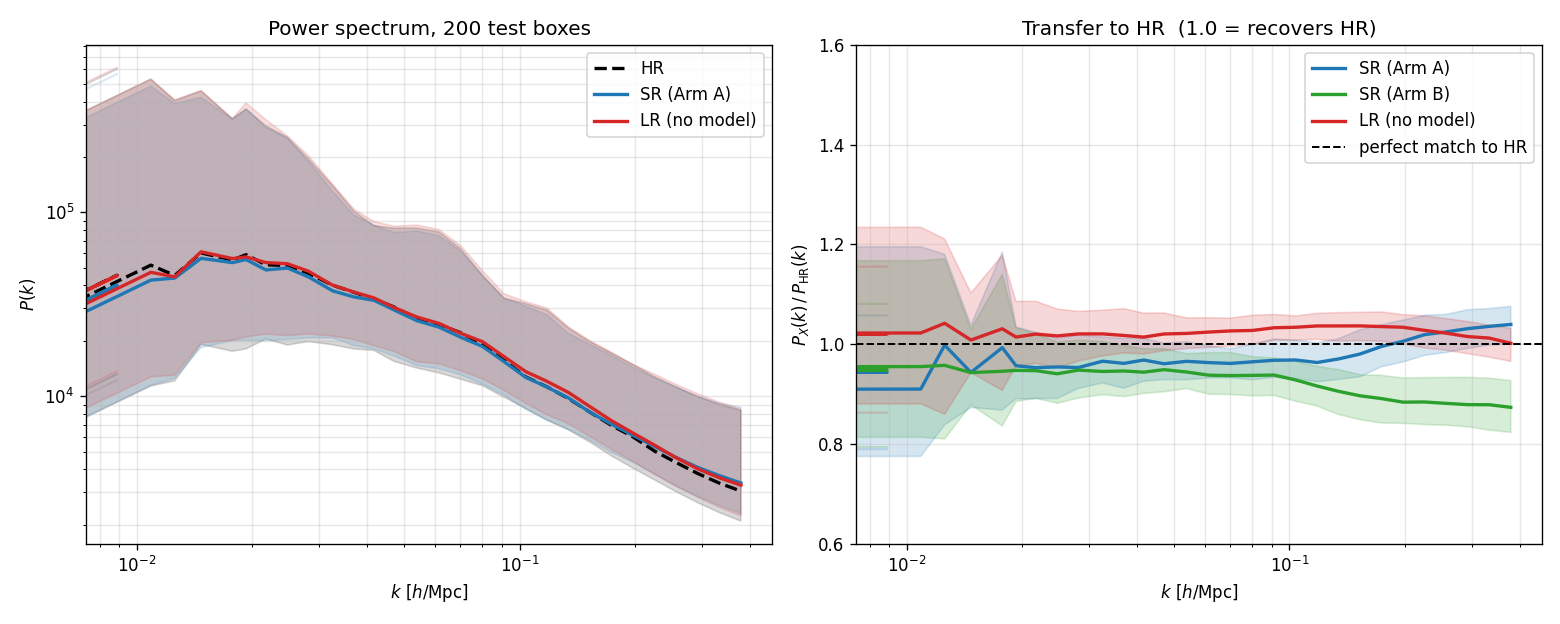
\includegraphics[width=0.98\linewidth]{figures_cmass/sr_vs_hr_pk.png}
\caption{\textbf{Left:} $P(k)$ of HR, SR (Arm A), and LR over $200$ test boxes
(median $+$ $16/84\%$ band). \textbf{Right:} transfer to HR; $1.0$ recovers HR.
SR (Arm A) sits near $1$ at all scales; Arm B's overlap blending slightly
suppresses small-scale power (transfer $0.88$).}
\label{fig:srs-srvshr}
\end{figure}

\paragraph{2. Field structure.} Beyond the power spectrum, SR keeps the field
structure of HR (Arm A, $16$ test boxes, \texttt{match\_stats\_cmassA.txt}):

\begin{table}[h]
\centering
\caption{SR vs HR field-match statistics (Arm A).}
\label{tab:srs-match}
\begin{tabular}{lll}
\toprule
quantity & value & reading \\
\midrule
total count ratio $\sum\mathrm{SR}/\sum\mathrm{HR}$ & $0.965\pm0.172$ & counts conserved on average; large per-box scatter \\
real-space std ratio & $1.008\pm0.100$ & clustering amplitude matches; not blurred \\
void fraction SR / HR ($<0.5$) & $0.855$ / $0.833$ & SR keeps voids empty, like HR \\
cross-coherence $r$, $k<0.05$ & $0.951$ & large-scale structure matches cell-by-cell \\
cross-coherence $r$, $k>0.2$ & $0.403$ & small-scale structure decorrelates \\
\bottomrule
\end{tabular}
\end{table}

\paragraph{3. Cosmology.} The cosmology comparison in the original report used
mislabeled cosmologies, an indexing bug we describe and fix in
\S\ref{sec:srs-correction}, so those numbers are not shown here. With correct
labels a single box constrains $\Omega_m$ and $\sigma_8$; at the power spectrum
level the raw LR field is already HR-like, while at the field level an SR-trained
posterior transfers to HR and an LR-trained one does not
(\S\ref{sec:srs-correction}, Table~\ref{tab:srs-corrected}).

\paragraph{4. Seam.} Neither arm introduces a stitching seam: the $x{=}64$
internal-seam excess is $\approx1$ for both
(Table~\ref{tab:srs-seam}, Fig.~\ref{fig:srs-seam}). Arm A shows a mild generic
ripple near \emph{any} boundary plane (seam-distance ratio $1.17$); Arm B's
overlap removes it ($1.00$) at a small cost in Pk RMS.

\begin{table}[h]
\centering
\caption{Seam and stitched-fidelity metrics, $200$ test boxes. ``Excess'' is
boundary error over interior error; $\approx1$ means no seam.}
\label{tab:srs-seam}
\begin{tabular}{lccp{5.2cm}}
\toprule
metric & Arm A naive & Arm B overlap & reading \\
\midrule
$x{=}64$ internal-seam excess & $0.9934$ & $0.9998$ & no internal seam either arm \\
seam-distance ratio ($d{=}0/d{\ge}8$) & $1.1729$ & $1.0032$ & generic boundary ripple, removed by overlap \\
$x{=}0$ periodic edge (control) & $0.9930$ & $0.9993$ & box edge behaves like interior \\
stitched PkRMS$_{\log_{10}}$ vs HR & $0.0637$ & $0.0678$ & stitched power-spectrum match \\
\bottomrule
\end{tabular}
\end{table}

\begin{figure}[t]
\centering
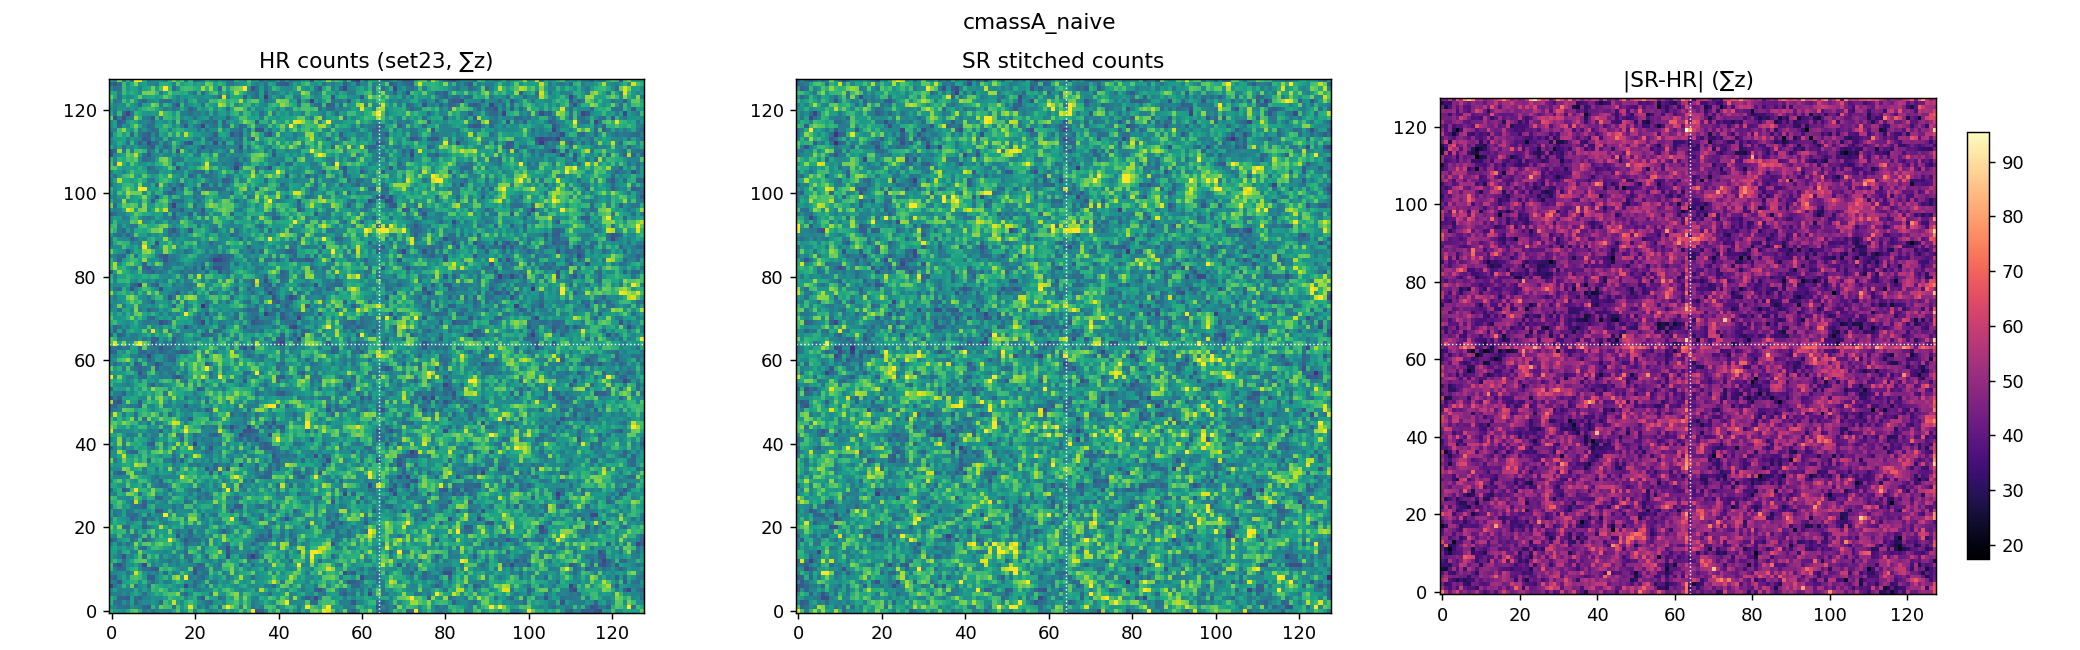
\includegraphics[width=0.95\linewidth]{figures_cmass/seam_cmassA_naive_slice.png}
\caption{Projected count maps for one test box (Arm A): HR, stitched SR, and the
absolute residual $|\mathrm{SR}-\mathrm{HR}|$. White dotted lines mark the
$x{=}64$, $y{=}64$ core boundaries; the residual shows no elevated ridge along
them.}
\label{fig:srs-seam}
\end{figure}

\paragraph{Per-scale diagnostic panels.} Figure~\ref{fig:srs-pkpanel} shows the
full-box $P(k)$, transfer, and cross-coherence for Arm A. The transfer sits near
$1$ at all scales (right amount of power); the cross-coherence is near $1$ at
large scales and falls toward small scales (structure placement is recovered at
large scales only). The per-patch panel
(\texttt{figures\_cmass/pk\_panel\_patch\_cmassAfix.png}) and the projection panels
(\texttt{projection\_box\_cmassAfix\_set23.png},
\texttt{projection\_patch\_cmassAfix\_set23\_p0.png}) tell the same story; Arm~B's
panels carry the \texttt{cmassB} suffix.

\begin{figure}[t]
\centering
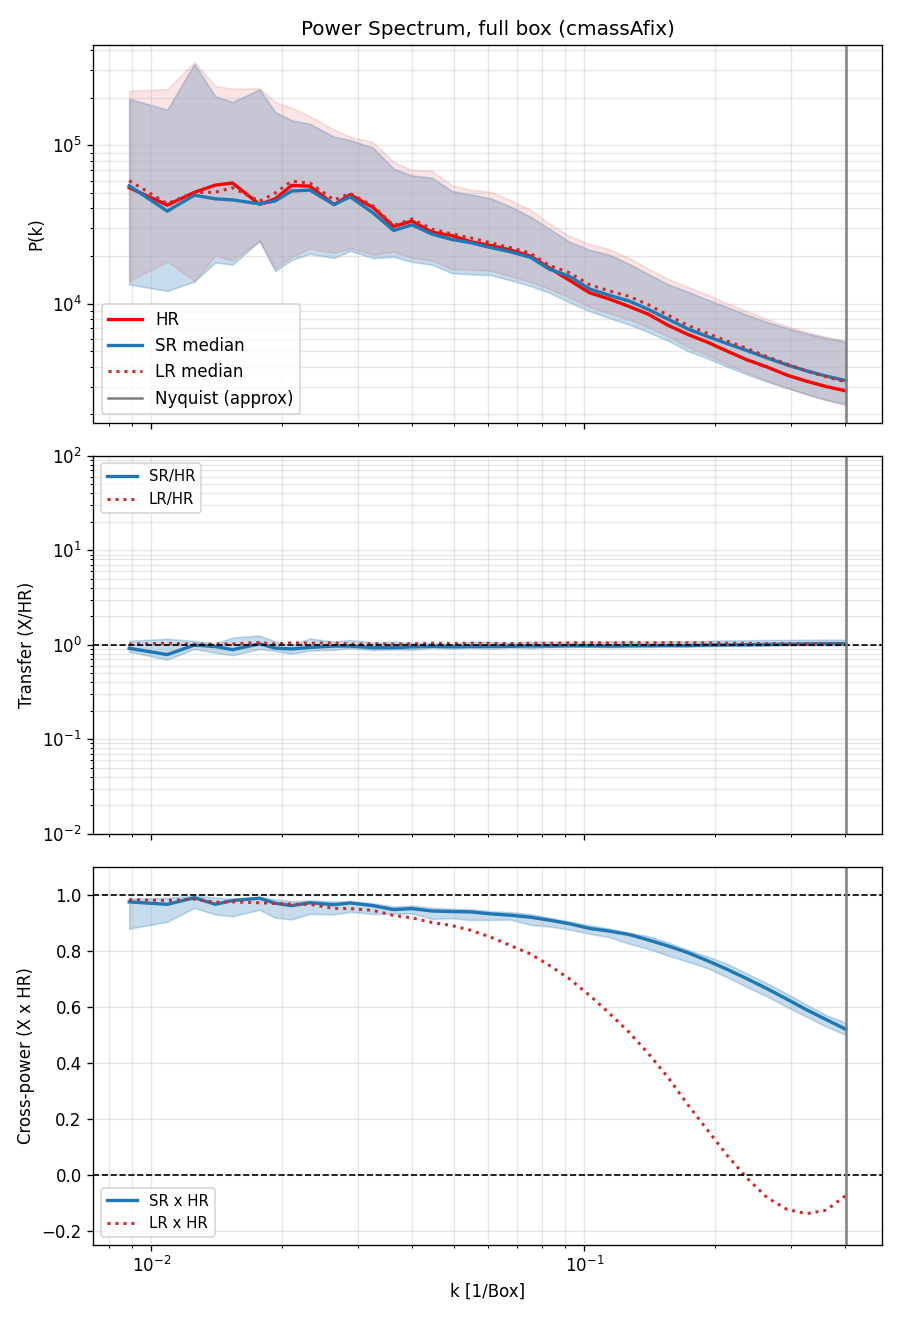
\includegraphics[width=0.5\linewidth]{figures_cmass/pk_panel_box_cmassAfix.png}
\caption{Full-box diagnostic for the conditioned generator (fiducial cosmology,
$16$ test boxes): $P(k)$ of HR (red), SR (blue median $+$ band), and LR (dotted
red); transfer $T(k)=P_X/P_\text{HR}$ on a linear axis with the 16 to 84
percentile band for both SR and LR, the legend reporting the RMS deviation of
each ratio from unity; and cross-coherence $r(k)$. The SR median transfer sits
below unity for $k<0.1$, a systematic large-scale power deficit of roughly 5 to
10 percent, while LR sits slightly above unity; SR does not tighten the transfer
scatter relative to LR. In $r(k)$, SR stays near unity to smaller scales while
LR decorrelates.}
\label{fig:srs-pkpanel}
\end{figure}

\subsection{Diagnostic: What is NOT Working}

\paragraph{Small-scale structure decorrelates, and this is fundamental.} SR
matches HR cell-by-cell at large scales ($r{=}0.95$ for $k<0.05$) but loses the
match at small scales ($r{=}0.40$ for $k>0.2$, Table~\ref{tab:srs-match}). This
is not a capacity bug: it is set by how much information the LR input carries
about HR. LR and HR share large-scale modes but the voxel-by-voxel LR$\leftrightarrow$HR
correlation is only $\approx0.06$, so the exact small-scale realization is simply
not present in the input. The model can match the small-scale \emph{statistics}
(transfer $\approx1$, real-space std ratio $1.008$) but cannot reproduce the
exact placement of individual halos. The noise injection
(Eq.~\ref{eq:srs-residual}) exists precisely because of this: it draws a
plausible small-scale field rather than regressing to a blur.

\paragraph{Per-box total-count scatter.} The total halo count is conserved on
average but with $\sim17\%$ per-box scatter ($\sum\mathrm{SR}/\sum\mathrm{HR}=
0.965\pm0.172$). A count-aware output head (predict a rate and sample Poisson
counts) would tighten this; it is the one clearly addressable imperfection. \SG{I would think this isn't necessary to fix, we don't care about the number of halos after all.}

\paragraph{Overlap suppresses small-scale power.} Arm B's overlap blending lowers
the small-scale transfer to $0.88$ (Table~\ref{tab:srs-pk}), so on the power
spectrum the naive Arm A is the better super-resolver. Overlap removes a small
generic boundary ripple but buys no fidelity, because on this continuous count
data there is no real seam to fix, the clean version of the mentor 2.1 vs 2.2
comparison.

\paragraph{Where the cosmology value is.} At the power spectrum level the raw LR
field is already close to HR, since they share large-scale modes, so the power
spectrum is a forgiving summary with little headroom. The model's value is at the
field level (variance, voids, small-scale structure), which the power spectrum
summary is insensitive to. The corrected cross-fidelity in
\S\ref{sec:srs-correction} bears this out: SR and LR are indistinguishable at the
power spectrum level, but at the field level an SR-trained posterior transfers to
HR while an LR-trained one does not.

\subsection{What I'm Trying Next}
\label{sec:srs-next}

The diagnostics above point to one limit that may be fundamental (small-scale
decorrelation) and a few that are clearly fixable (count scatter, small-scale
realism). The plan below is ordered so that we \emph{measure} the limit before
spending effort trying to beat it. None of these results are in yet; this is the
roadmap, not an experiment log.

\paragraph{Step 0, measure the information ceiling first.} Before trying to
improve the small-scale match, we need to know whether $r{=}0.40$ at small scales
(Table~\ref{tab:srs-match}) is the best any model could do from this input, or a
weakness of the current one. Two cheap diagnostics settle it:
\begin{itemize}
  \item \textbf{LR$\leftrightarrow$HR cross-coherence $r_\text{LR,HR}(k)$.} The
  cross-coherence of the \emph{raw input} against HR (no model) is the ceiling:
  no function of LR can place small-scale structure better than the input
  already correlates with HR. If $r_\text{SR,HR}(k)\approx r_\text{LR,HR}(k)$ at
  small $k$, the model is already at the ceiling and the limit is fundamental;
  if it sits well below, there is recoverable structure left on the table. (Only
  per-box $P(k)$ is currently saved, not the cross-spectrum, so this needs one
  re-run that keeps the fields.)
  \item \textbf{No-noise ablation.} Train the same generator with the noise
  injection off (a plain regressor). Theory predicts this should \emph{raise} the
  small-scale cross-coherence a little (a regressor targets the conditional mean,
  the best cell-by-cell predictor) but \emph{lower} the small-scale transfer well
  below $1$ (the conditional mean is blurry). Seeing exactly that trade-off would
  confirm that the noise/GAN is the right choice for a power-spectrum target, and
  would quantify how much cell-by-cell accuracy is being traded for correct
  statistics.
\end{itemize}

\paragraph{Step 1, fix the count scatter and small-scale realism (independent
of the ceiling).} These help regardless of what Step 0 finds:
\begin{itemize}
  \item \textbf{Count-aware (Poisson) output head.} Instead of predicting a
  count directly, predict a non-negative rate $\lambda$ per cell and sample the
  count as $n\sim\mathrm{Poisson}(\lambda)$. Halo counts are discrete and sparse,
  so a Poisson head models the small-scale graininess as actual shot noise rather
  than a smeared residual, and should tighten the $\sim17\%$ per-box total-count
  scatter (Table~\ref{tab:srs-match}), the one clearly addressable imperfection.
  \item \textbf{Explicit statistics terms in the loss.} Add a one-point PDF /
  variance matching term so small-scale sharpness is enforced directly, rather
  than relying on the adversarial term alone to find it.
  \item \textbf{Loss rebalance.} The current weights are $\lambda_\text{rec}{=}2$,
  $\lambda_\text{pk}{=}2$, $\lambda_\text{adv}{=}1$
  (Eq.~\ref{eq:srs-lossG}). The $L_1$ term blurs; lowering it and raising the
  adversarial weight should push toward correct statistics, at a known cost in
  cell-by-cell accuracy, per the same trade-off as the no-noise ablation.
\end{itemize}

\paragraph{Step 2, extract more of the available information (only if Step 0
shows headroom).} If $r_\text{SR,HR}$ sits below the LR$\leftrightarrow$HR
ceiling, the model is under-using its input. A larger receptive field, or feeding
each patch more neighbour context, would let it use more of the LR field to
predict the residual. This only helps if there is headroom to recover.

\paragraph{Step 3, raise the ceiling by changing the \emph{input}, not the
model.} The small-scale cell-by-cell limit is set by the information in the LR
input (the voxel-by-voxel LR$\leftrightarrow$HR correlation is only
$\approx0.06$). No amount of model capacity raises that; only more informative
inputs do. Candidates: feed the shared small-scale \emph{initial conditions}
(which the coarse LR count field has discarded), or add the LR velocity / particle
fields. This is the only route to a meaningful gain in small-scale cross-coherence,
and is the natural bridge to the displacement-field model of \S5, which already
carries that extra information.

\paragraph{Summary.} Steps 0--1 are the near-term plan: measure the ceiling, then
add a Poisson head and statistics losses to fix the count scatter and sharpen the
small-scale field. Steps 2--3 are contingent on what Step 0 reveals. For a
cosmology deliverable the priority is statistical fidelity (which Steps 0--1
target); exact small-scale reconstruction (Step 3) is a larger, input-level
change worth it only if cell-by-cell recovery becomes the goal.

\subsection{Follow-Up Results: New Protocol from the Mentor Meeting}
\label{sec:srs-followup}

A mentor meeting after the report above changed two things about how we train
and evaluate this model. First, the real goal is not to match HR with SR by
itself. The real goal is to train a posterior model on SR output and have it
work well when it is tested on real HR data, since HR simulations are too
expensive to train a posterior model on directly. Second, the power spectrum
term was removed from the training loss, since it was also our main success
metric and that is a weak test. This subsection reports what we found. Some of
the training runs below are still in progress at the time of writing, so
numbers marked as current are read from the latest completed epoch, not a
final result.

\paragraph{Held-out check: the bispectrum.} A fair worry is that our power
spectrum result looks good only because the power spectrum was also in the
training loss. To check this we measured the bispectrum, a higher-order
statistic that was never used anywhere in training or model selection. If SR
only matches the power spectrum and nothing else, the bispectrum should show
no improvement over the raw LR input.

\begin{figure}[t]
\centering
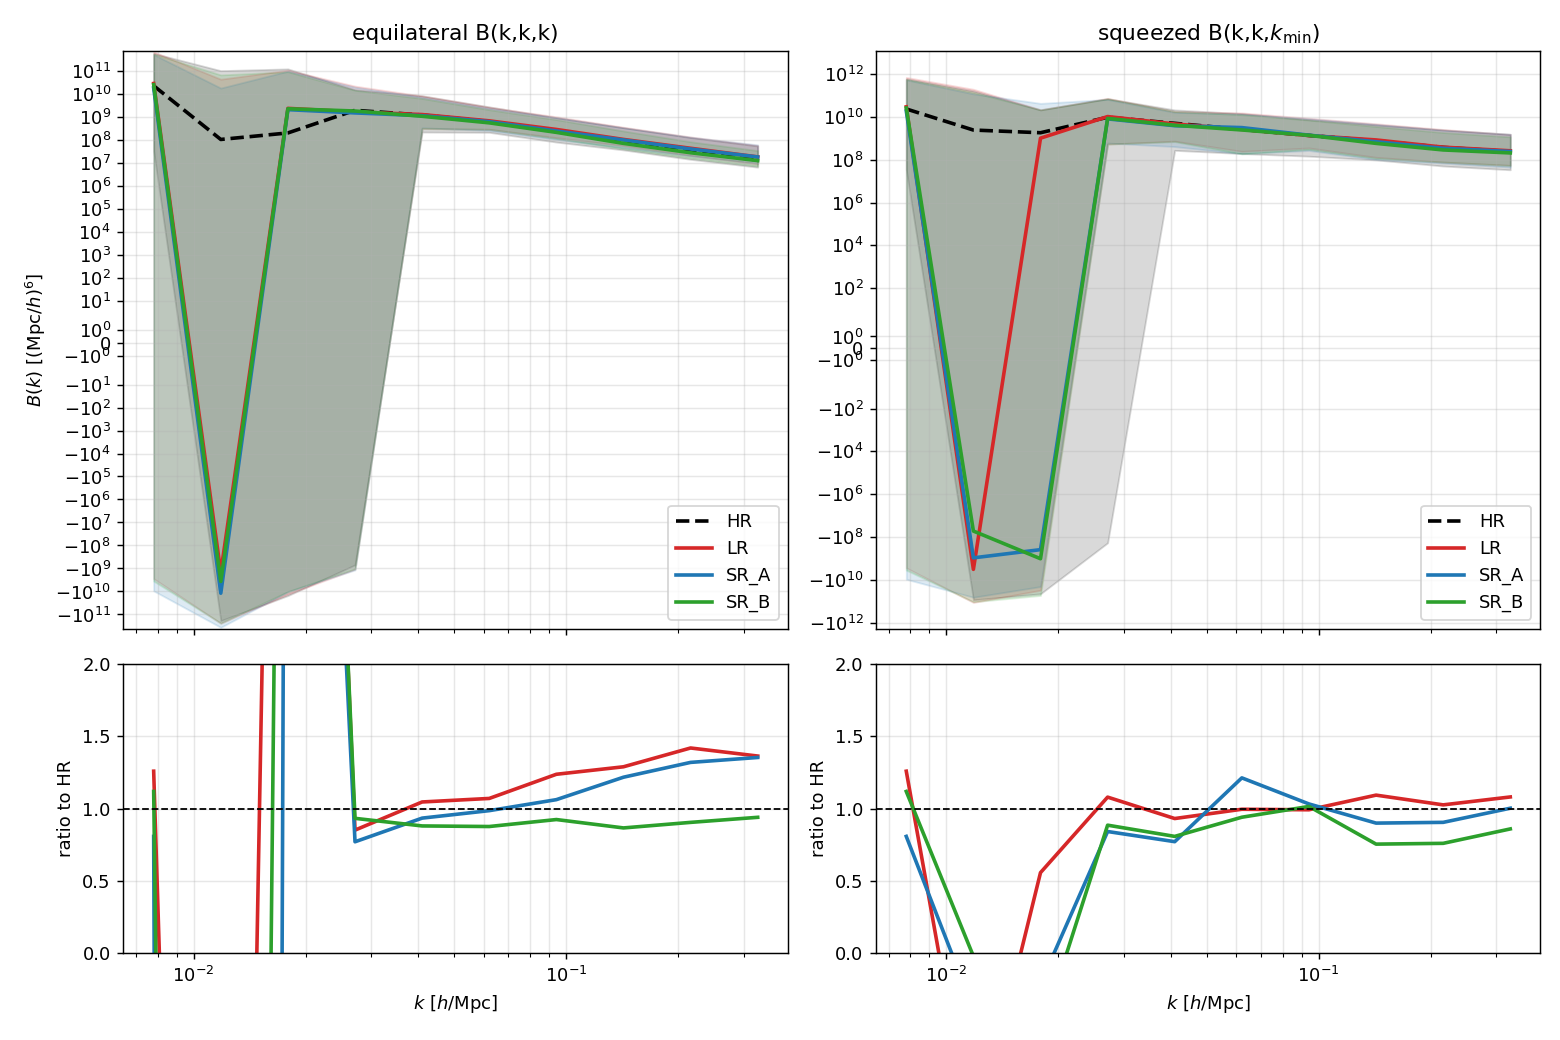
\includegraphics[width=0.95\linewidth]{figures_cmass/bispectrum_hr_lr_srA_srB.png}
\caption{Bispectrum of HR, LR, and SR (both arms), on $16$ test boxes. Top:
equilateral and squeezed bispectrum, HR in black. Bottom: ratio to HR. SR
removes most of the systematic excess that LR has at the plotted scales,
without ever training on this statistic.}
\label{fig:srs-bispec}
\end{figure}

On the equilateral configuration, LR sits about $6$ to $13$ percent above HR
across the middle range of scales. SR removes most of this gap without ever
seeing a bispectrum during training, and it does this for both arms. This is
evidence that the model is not simply fitting the training metric. It is
correcting real structure in the field that also shows up in a statistic it
never saw. (The figure uses the earlier models trained \emph{with} the power
spectrum loss; the no-Pk models of the following paragraphs preserve the
bispectrum at least as well, so removing that loss did not degrade this
held-out statistic either.)

\paragraph{Removing the power spectrum loss.} Following the meeting, we
retrained the model with the power spectrum term switched off
($\lambda_\text{pk}{=}0$ in Eq.~\ref{eq:srs-lossG}), so the loss is only the
adversarial and $L_1$ terms. We also changed which checkpoint counts as "best"
to the real-space $L_1$ error, since selecting on the power spectrum would
have been the same kind of leak we were trying to remove.

\begin{figure}[t]
\centering
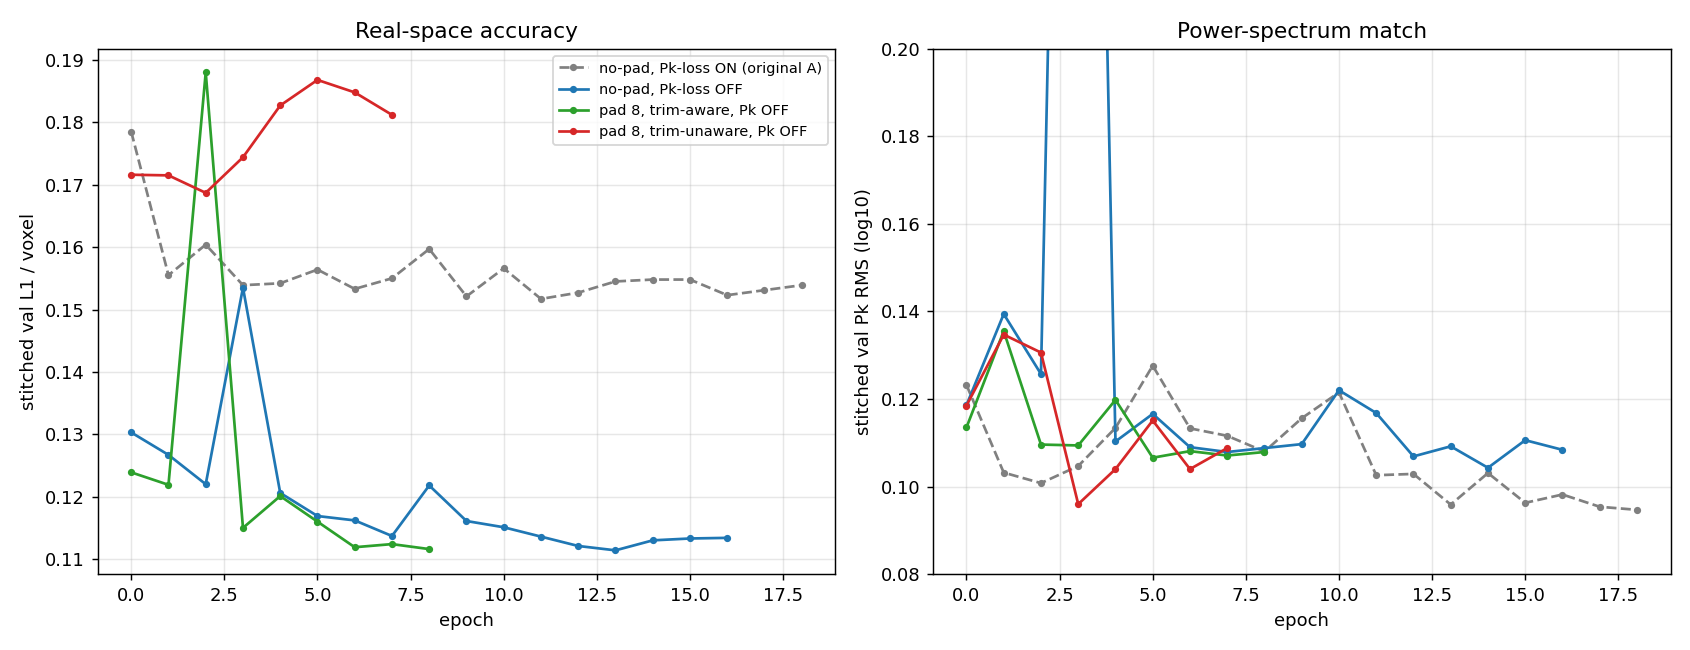
\includegraphics[width=0.98\linewidth]{figures_cmass/protocolv2_cmass.png}
\caption{Stitched validation curves under the new protocol (power spectrum
loss off). Left: real-space $L_1$ error. Right: power spectrum RMS error. Grey
dashed: the original Arm A with the power spectrum loss on, for comparison.
These runs are still training; curves stop at the most recent completed
epoch.}
\label{fig:srs-protocolv2}
\end{figure}

Two things stand out so far. First, without the power spectrum term, the
real-space $L_1$ error becomes clearly better than the original run at the
same point in training (left panel, blue and green curves sit below the grey
dashed curve). Second, the power spectrum error does get a little worse
without its loss term, but it does not collapse: it settles into roughly the
same range as before, just a bit noisier. So the power spectrum term was
buying us a small amount of power spectrum accuracy at a real cost in
real-space accuracy. It was not the only reason the power spectrum matched
well; the adversarial and reconstruction terms carry most of that on their
own.

\paragraph{Does padding help, once the power spectrum loss is out of the way?}
The report above found that padding (Arm B) did not beat no padding (Arm A) on
the power spectrum. The mentor pointed out two different ways this could
happen, and that they make different, testable predictions:
\begin{itemize}
  \item \textbf{Trim-aware.} The model is trained knowing that only the middle
  part of its output will be kept; the loss only looks at that middle part.
  This is what Arm B already did. If this is working correctly, padding should
  train at least as well as no padding, since it has strictly more context for
  the same target.
  \item \textbf{Trim-unaware.} The model is trained as if its whole padded
  output matters, including the edge region that gets thrown away later. If
  the model leans on that edge region during training, it should look fine
  during training but generalize worse once the edge is cut off at test time.
\end{itemize}
We trained both versions with the power spectrum loss off, so the comparison
is not confused by that term. Figure~\ref{fig:srs-protocolv2} shows all three
runs together (no padding, trim-aware padding, trim-unaware padding).

The trim-aware version (green) matches or beats no-padding (blue) on both
real-space error and power spectrum error at almost every epoch measured so
far. This supports the first prediction: once the model is told correctly what
part of its output is graded, more context helps rather than hurts. The
trim-unaware version (red) is clearly worse on real-space error than both
other runs, and does not close that gap as training continues. This supports
the second prediction: a model that is allowed to rely on the part of its
output that gets discarded at test time pays for that at test time. Put
together, the original result that padding did not help was most likely
caused by the power spectrum loss, not by padding itself.

We also reran the older, padding-with-power-spectrum-loss model for more
epochs to check whether it had simply not been trained long enough. Fifteen
additional epochs did not beat its early best score, so that run was not
undertrained; the training recipe, not the training time, was the limiting
factor.

\subsection{The Goal Metric: Corrected Cross-Fidelity Results}
\label{sec:srs-correction}

\paragraph{The bug.} After the analysis above, a routine physical sanity check
failed in a way that could not be real: the amplitude of the power spectrum had
essentially zero correlation with $\sigma_8$, and a fit of the power spectrum to
the five parameters explained only $0.2\%$ of the variance. The power spectrum
amplitude must scale with $\sigma_8$, so this pointed to a labeling error, not to
physics. Tracing it, we found that the processed count fields were written in
string-sorted simulation order ($0, 1, 10, 100, 1000, \dots$) while the cosmology
table is indexed numerically. Field number $k$ is therefore the halo field of
simulation string-sort$(k)$, not simulation $k$, so every field in the whole
pipeline was paired with the wrong cosmology. We proved this exactly: using the
original halo catalogs, the field halo count matches the catalog count under the
string-sort permutation for all $2000$ simulations, while the identity mapping
matches only the two fixed points. We corrected the cosmology table to field
order, backed up the old one, and patched the builder so it cannot regenerate the
wrong order.

\begin{figure}[h]
\centering
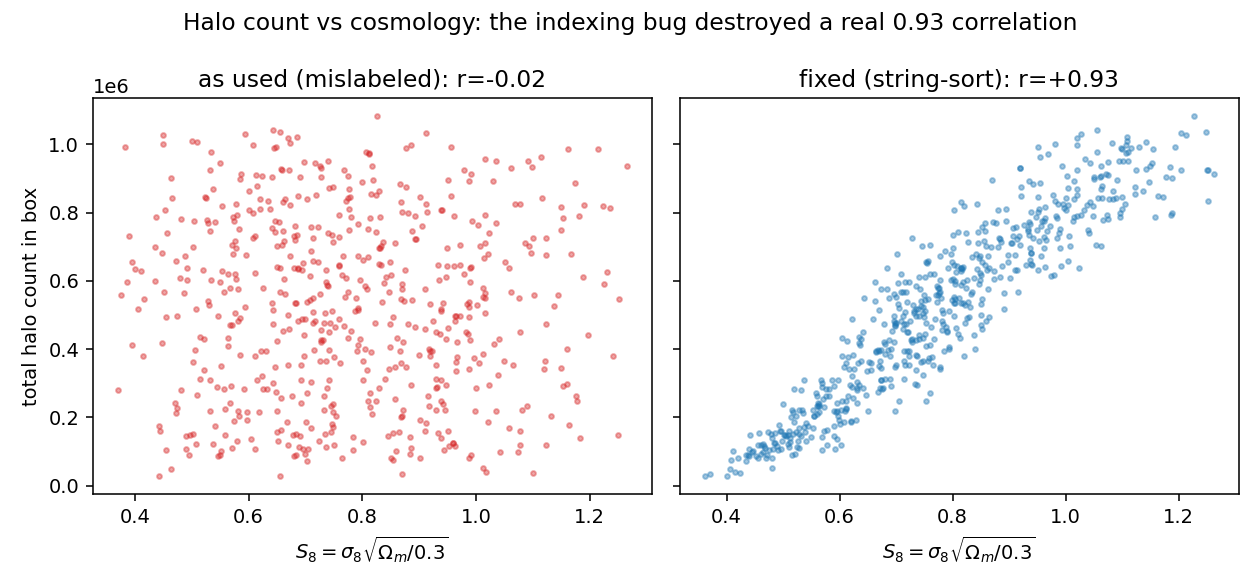
\includegraphics[width=0.85\linewidth]{figures_cmass/labelbug_count_vs_s8.png}
\caption{The indexing bug in one picture. Total halo count in a box against
$S_8 = \sigma_8\sqrt{\Omega_m/0.3}$. As the pipeline used the labels (left) the
correlation is zero; with the string-sort mapping corrected (right) the true
$0.93$ correlation reappears. Halo abundance must track $S_8$, so the left panel
was the signature of a labeling error, not of uninformative data.}
\label{fig:srs-labelbug}
\end{figure}

\paragraph{What this changes, and what it does not.} Every cosmology number we
computed before this point used the labels and is affected; the earlier
cross-fidelity tables have been removed and are replaced by the corrected results
below, and the earlier reading that the SR-versus-LR difference was an irreducible
coin flip was itself a product of the mislabeling. The results that do not use the
labels are unaffected and still stand: the power spectrum match of SR to HR, the
held-out bispectrum, the field-match statistics, the seam test, and the real space
error. The generator conditions on the cosmology as a style vector and was trained
with the scrambled labels, so its conditioning was uninformative during training;
we return to this at the end.

\paragraph{The data is informative after all.} With correct labels the picture
inverts. A halo count in this suite carries a strong cosmological signal: the
total halo count alone correlates with the combination $S_8 = \sigma_8
\sqrt{\Omega_m/0.3}$ at $0.93$ and with $\Omega_m$ at $0.85$. A Fisher forecast on
a single-box power spectrum now explains $98\%$ of the variance, where it
explained $0.2\%$ before, and it constrains $\Omega_m$ and $\sigma_8$ well, with
$\Omega_b$, $h$ and $n_s$ weak or unconstrained, which is the textbook pattern for
a low-redshift halo field. The field-level network tells the same story: after the
fix its predicted $\Omega_m$ correlates with the truth at $0.90$ on both training
and test boxes, where before the fix the correlation was zero and the output was a
constant. So the earlier conclusion that a single box carries almost no cosmology
was an artifact of the labeling, not a property of the data.

\begin{figure}[h]
\centering
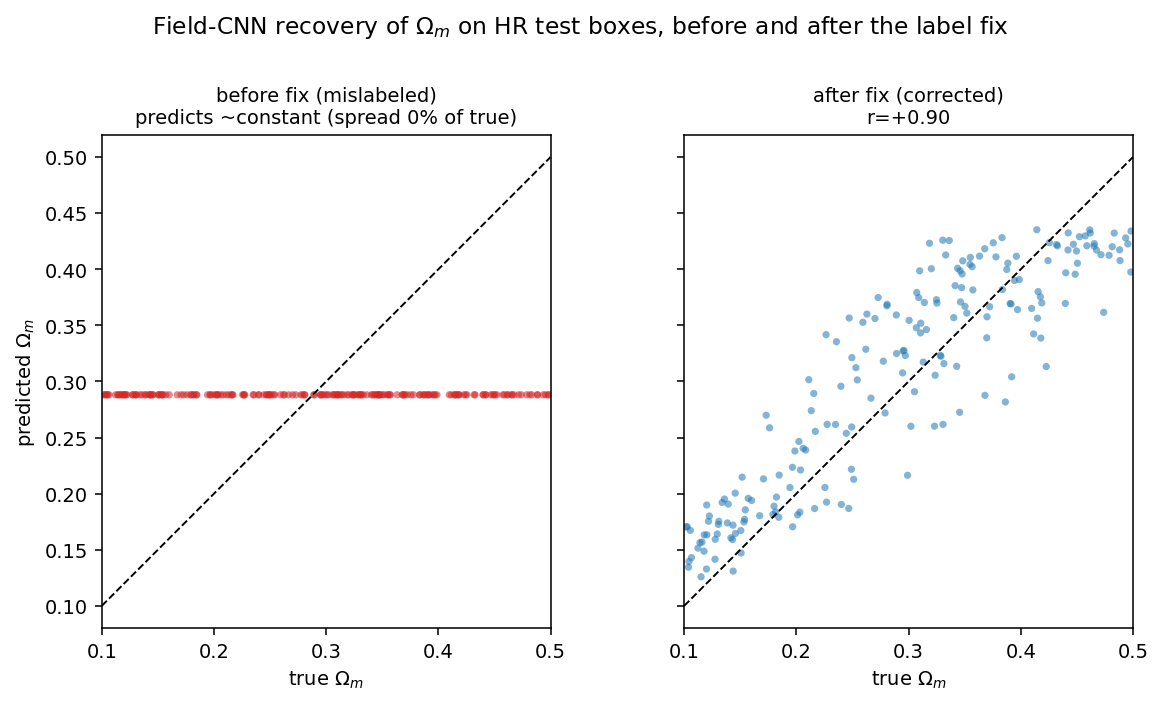
\includegraphics[width=0.82\linewidth]{figures_cmass/field_recovery_Om_cmass.png}
\caption{Field-level CNN recovery of $\Omega_m$ on HR test boxes, before and after
the label fix. Before (left) the prediction is flat and uncorrelated with the
truth (the network returns a near-constant); after (right) it tracks the diagonal
at a correlation of about $0.90$, on both training and test boxes. Same
architecture, same data, only the labels changed.}
\label{fig:srs-recovery}
\end{figure}

\begin{figure}[h]
\centering
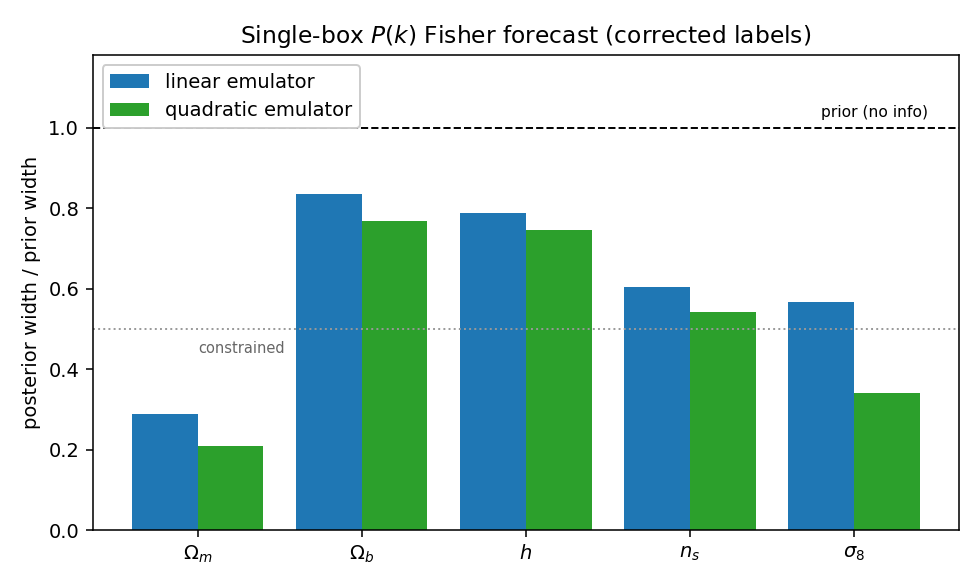
\includegraphics[width=0.72\linewidth]{figures_cmass/fisher_corrected_cmass.png}
\caption{Fisher forecast for a single-box power spectrum with corrected labels:
posterior width divided by prior width per parameter (lower means better
constrained, $1$ means no information). $\Omega_m$ is well constrained and
$\sigma_8$ is constrained, while $\Omega_b$, $h$ and $n_s$ are weak, the textbook
pattern for a low-redshift halo field. Two emulators (linear average slope and
quadratic at the prior centre) bracket the estimate.}
\label{fig:srs-fisher}
\end{figure}

\paragraph{Corrected cross-fidelity, and where SR helps.} We re-ran the goal
metric with correct labels at two levels, the power spectrum summary and the full
field. We train the posterior on one source, apply it to HR, and compare to a
posterior trained on HR, using an ensemble of independently retrained estimators
so the numbers are not single draws. Table~\ref{tab:srs-corrected} gives the
result.
\begin{table}[h]
\centering
\caption{Corrected cross-fidelity KL to HR (posterior trained on the named source,
evaluated on HR), lower is better, with the HR-to-HR floor for reference. Summary
uses the power spectrum; field uses a three-dimensional CNN posterior on the full
box.}
\label{tab:srs-corrected}
\begin{tabular}{lccc}
\toprule
level & LR (raw) & SR & HR floor \\
\midrule
summary $P(k)$ & $0.032$ & $0.088$ & $0.028$ \\
field (CNN)    & $0.49 \pm 0.81$ & $\mathbf{0.024}$ & $0.022$ \\
\bottomrule
\end{tabular}
\end{table}
\begin{figure}[h]
\centering
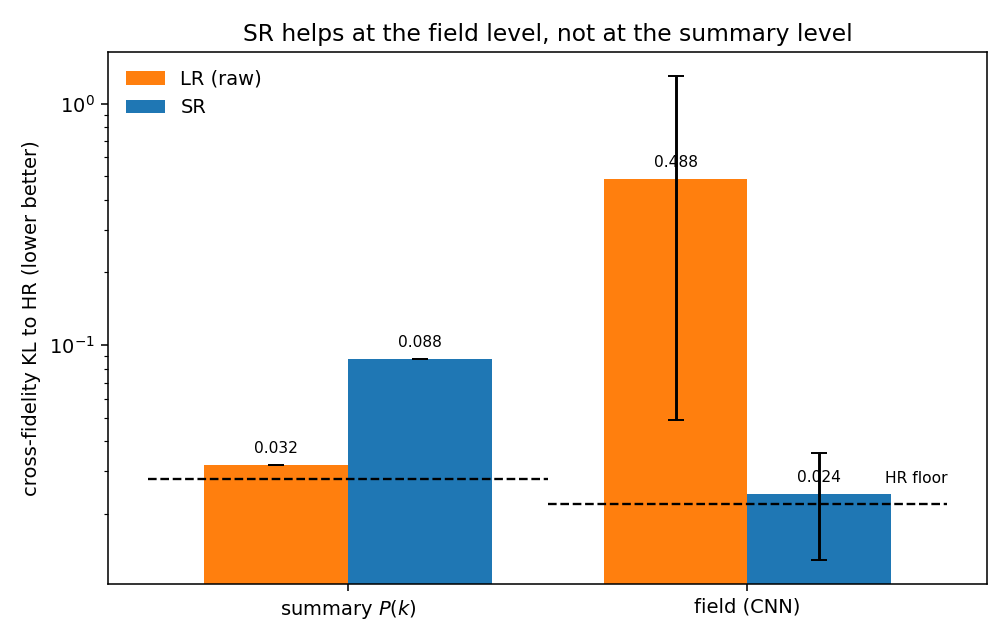
\includegraphics[width=0.7\linewidth]{figures_cmass/crossfid_corrected_cmass.png}
\caption{Corrected cross-fidelity KL to HR (log scale, lower is better) at the two
levels, with the HR-to-HR floor shown as the dashed line. At the summary level the
raw LR field is already at the floor and SR does not help. At the field level, an
LR-trained posterior does not transfer to HR (large and unstable), while an
SR-trained posterior sits at the floor. SR helps exactly where it corrects the
field.}
\label{fig:srs-crossfid-corrected}
\end{figure}
The two levels point in opposite directions, and both make sense. At the summary
level the raw LR power spectrum is already at the HR floor, so an LR-trained
posterior transfers to HR as well as an HR-trained one does, and there is no gap
for SR to close; SR even hurts a little, because the generator reshapes the
small-scale power in a way that does not match how HR responds to cosmology. At
the field level the raw LR box looks different enough from HR that an LR-trained
posterior does not transfer, and it does so unreliably, sometimes acceptably and
sometimes catastrophically, which is why its number carries such a large spread.
SR corrects the field to look like HR, so an SR-trained posterior transfers to HR
reliably, at the floor. This is exactly the deployment case the project is built
on, train the inference model on cheap SR-corrected boxes and apply it to
expensive HR, and at the field level SR makes it work where raw LR does not.

\paragraph{Padding on the goal metric.} We ran the two padding variants through
the corrected cross-fidelity at the summary level as well
(Table~\ref{tab:srs-padding}). Among the SR models the ordering from the earlier
report survives: no padding is best on the goal metric, trim-aware padding is
worse, and trim-unaware is worst, so for the cosmology objective the no-padding
model is the one to use. All three sit above the raw LR control at this level,
consistent with LR already being HR-like on the power spectrum. One number does
change under the fix: the mislabeled data made trim-unaware look catastrophic (a
factor of several hundred above the others), while with correct labels it is the
weakest variant by about a factor of two, not a blow-up. Its real-space error
(Figure~\ref{fig:srs-protocolv2}) remains the clearest and most direct sign that
it is the least reliable model.
\begin{table}[h]
\centering
\caption{Corrected cross-fidelity KL to HR at the summary (power spectrum) level
for the SR padding variants, with the LR control and the HR floor. Lower is
better. Field-level padding numbers are future work.}
\label{tab:srs-padding}
\begin{tabular}{lc}
\toprule
model & summary cross-fidelity KL \\
\midrule
SR, no padding & $\mathbf{0.087}$ \\
SR, trim-aware padding & $0.127$ \\
SR, trim-unaware padding & $0.172$ \\
\midrule
LR (control) & $0.031$ \\
HR floor & $0.028$ \\
\bottomrule
\end{tabular}
\end{table}

\paragraph{Bottom line.} With the labels fixed, the cosmology question has a
clear answer. The data constrains $\Omega_m$ and $\sigma_8$ from a single box. At
the power spectrum level the raw LR field is already HR-like, so SR is not needed
there and slightly hurts. At the field level, which is what SR actually corrects,
an SR-trained posterior transfers to HR at the floor while a raw LR one does not,
so SR provides a real and reliable cosmology benefit exactly where it operates.
Trim-unaware padding is still the weakest variant, worst on the goal metric and
on real-space error, though the label fix shrinks its apparent failure from
catastrophic to about a factor of two. Two honest caveats remain: the
field-level LR number has a wide spread and rests on a handful of retrained
networks, so the size of the gap should be firmed up with more seeds; and because
the generator was trained with the scrambled labels, its cosmology conditioning
was uninformative, so a retrain with correct conditioning may sharpen the SR
result further. Neither caveat changes the direction: with correct labels, SR
helps cosmology at the field level.

\paragraph{A data reliability note.} Partway through these runs, the shared
data storage this project reads from filled up completely, which caused a few
training jobs to fail with a file briefly appearing missing even though it was
not actually deleted. We added a retry step to the data loader and resumed
each affected run from its last saved checkpoint, so no real training progress
was lost. This is a shared infrastructure issue, not a problem with the data or
the method.

\subsection{Files}
\begin{itemize}\itemsep0pt
  \item Data and patching: \texttt{data/patch\_dataset\_cmass.py}
  (shared ops in \texttt{data/patch\_dataset\_real.py})
  \item Model: \texttt{map2map/models/styled\_srsgan.py}
  (\texttt{G\_correct}, \texttt{D\_const})
  \item Training: \texttt{train\_patch\_cmass.py};
  run script \texttt{scripts/train\_patch\_cmass.slurm}
  \item Inference and stitching: \texttt{infer\_stitch\_cmass.py}
  \item Seam eval: \texttt{analysis/eval\_seam\_cmass.py}
  \item Box / per-patch diagnostics: \texttt{analysis/diag\_cmass.py}
  \item SR-vs-HR match stats: \texttt{analysis/match\_stats\_cmass.py}
  \item SR-vs-HR power-spectrum figure: \texttt{analysis/plot\_sr\_vs\_hr.py}
  \item Bispectrum (held-out statistic): \texttt{analysis/bispectrum\_cmass.py}
  \item Training loss curves: \texttt{analysis/plot\_losses\_cmass.py}
  \item Cross-fidelity posterior evaluation: \texttt{evaluate.py} (SR-trained
  or LR-trained posterior evaluated on HR $P(k)$)
  \item Protocol-v2 (no-Pk-loss, padding-variant) training curves:
  \texttt{analysis/plot\_protocolv2\_cmass.py}
  \item Power spectrum on counts: \texttt{analysis/power\_spectrum.py}
  (estimator \texttt{counts}); differentiable training version
  \texttt{analysis/pk\_torch.py}
  \item Posterior and KL: \texttt{inference/nde.py}, \texttt{evaluate.py};
  end-to-end eval \texttt{scripts/eval\_cmass\_wrapper.slurm}
  \item Field-level posterior (three-dimensional CNN, moment-network loss):
  \texttt{models/field\_cnn.py}, \texttt{train\_field\_cnn.py};
  SR field generation \texttt{gen\_sr\_fields.py}; capacity and recovery
  diagnostics \texttt{overfit\_test.py}, \texttt{field\_diag.py}
  \item Outputs: \texttt{runs/patch\_cmass/}; figures: \texttt{figures\_cmass/}
\end{itemize}
.
% Needs the packages main.tex already loads (booktabs, algorithm, algpseudocode,
% listings, xcolor, graphicx). Figures live in figures_cmass/.
% Numbers (updated 2026-09-28, see research_scratch_5.md): summary cross-fid from
% logs/3248394_seedxfid.log (nde_v2, 8 seeds for the main arms) and
% logs/3200801_seedxfid.log (4-seed ablation rows); field cross-fid from
% logs/3248260_fieldev.log (Flow+GAN, 40 epochs), logs/3203212_fieldev.log (20 epochs)
% and the other *_fieldev.log files; scale-by-scale from scratch/why/coh.py
% (COH_SPLIT=test, 200 test boxes); posterior shifts from scratch/why/post_diag_any.py
% (logs/3249151_postdiag.log, logs/3251464_postdiag.log); PQMass, bispectrum and halo
% counts from logs/*_tier1.log; calibration from logs/3251512_spread.log; figures from
% flow_matching/plot_sec7.py. LR here is CHARM (section6_srs.tex calls it FastPM,
% which is wrong).
% =====================================================================

\definecolor{ablgood}{HTML}{1B7F1B}
\newcommand{\abgood}[1]{\textcolor{ablgood}{\textbf{#1}}}

\section{Flow+GAN: Flow Matching Started from the GAN}
\label{sec:flowgan}

This section documents the third model in this work at the same level of detail
as \S\ref{sec:srs}. \S\ref{sec:srs} corrects the LR halo count field with a
styled GAN. The GAN makes the field look like HR, but it is deterministic, and
it biases the summary-level cosmology posterior. Here we keep that GAN and add a
conditional \textbf{flow-matching} model on top of it. The flow starts from the
GAN's output plus noise and learns to turn it into a sample of the HR field. We
call the combined model \textbf{Flow+GAN}. The section ends with a table of
every model and ablation we ran on this data (\S\ref{sec:flowgan-ablations}).

\paragraph{Goal.} The goal is the same as in \S\ref{sec:srs}. At inference the
model sees only the cheap LR field and must produce an SR field that behaves like
HR. We grade it the same way: a posterior trained on SR fields is applied to HR
fields, and we measure how far its answer is from a posterior trained on HR
(cross-fidelity KL). HR is used only for training and grading.

\paragraph{Why a new model: what the GAN and a plain flow get wrong.} Two
findings from the previous section and its follow-ups motivate this design.
\begin{itemize}
  \item \textbf{The GAN is deterministic and tilts the power spectrum.} Its
  learned noise strength is about $2\times10^{-4}$, so ten noise draws give the
  same field. Its $L_1$ term pulls each voxel toward the conditional median.
  This shrinks the large-scale contrast (about $5\%$ less power at $k<0.06\,h\,\mathrm{Mpc}^{-1}$)
  and adds $1$ to $3\%$ power at high $k$. A posterior reads this tilt as a
  shift in $\sigma_8$: on HR test boxes the GAN-trained posterior's $\sigma_8$ mean
  is off by about one HR posterior width. That is why the deployed GAN's summary
  cross-fidelity KL ($0.202$) is worse than raw LR ($0.049$). One fixed per-$k$
  calibration curve on the GAN's training $P(k)$ brings it to $0.068$, which
  shows the problem is this tilt, not missing information.
  \item \textbf{A plain flow samples, but loses the large scales.} A flow that
  starts from pure Gaussian noise (``Flow'' below) has no $\sigma_8$ bias and
  reaches $0.087$. But it rebuilds every scale from noise, including the largest
  ones, which LR already gets right. Its large-scale power scatters more from box
  to box than LR's. Its coherence with HR at $k\approx0.125$ falls below LR's.
  Its predictions are also too narrow: HR usually falls outside the spread of its
  draws (spread-skill ratio $0.20$, ideal $1$).
\end{itemize}
Flow+GAN takes the part each model gets right. The GAN supplies the large-scale
structure and a best guess. The flow adds only what the best guess cannot
predict, and it adds it as a sample, not as a mean. This follows residual
diffusion for downscaling (CorrDiff, Mardani et al.\ 2023, arXiv:2309.15214),
stochastic flow matching for super-resolution (Fotiadis et al.\ 2024,
arXiv:2410.19814), and stochastic interpolants with a data-dependent start
(Albergo et al.\ 2023, arXiv:2310.03725).

\paragraph{Terminology.} \textbf{GAN} means the deployed generator of
\S\ref{sec:srs}: Arm A (pad $0$), power-spectrum loss off, trained with correct
cosmology labels, run at the fiducial cosmology (tag \texttt{Afixfid}).
\textbf{Flow} means the pure-noise flow matcher trained on $64^3$ patches (tag
\texttt{fm\_gauss\_nodq}). \textbf{Flow+GAN} is the model of this section. As in
\S\ref{sec:srs}, we use LR/LF and HR/HF interchangeably.

\subsection{Data Preprocessing}
\textit{Source: \texttt{cmass-ili}; loaders \texttt{flow\_matching/data.py}
(\texttt{FullBoxDataset}), model space \texttt{flow\_matching/space.py}.}

\paragraph{Input.} The data is the same as in \S\ref{sec:srs}: $2000$ paired
halo count grids of $128^3$ cells on a periodic $1000\,h^{-1}\mathrm{Mpc}$ box at
$z=0.5$, with LR from CHARM and HR from Quijote N-body, and the same
$1600/200/200$ train/validation/test split. One extra input is new. Before
training, we run the GAN once on every one of the $2000$ LR boxes, at the
fiducial cosmology, and store its output (\texttt{sr\_fields/Afix\_fiducial}).
The GAN is frozen from here on; it is not trained further.

\paragraph{Model space.} The flow works on a standardised log count,
\begin{equation}
  y = \frac{\log(1+n) - \mu}{s}, \qquad
  n = \mathrm{round}\big(\exp(s\,y+\mu) - 1\big) \ \ \text{clamped to } [0, 200],
  \label{eq:fg-space}
\end{equation}
where $\mu=0.152$ and $s=0.359$ are the mean and standard deviation of
$\log(1+n_\text{HR})$ over $50$ training boxes. The LR field, the GAN field and
the HR target all use this same map. We do \emph{not} dequantise (add uniform
noise to the integer counts before the log). An earlier flow that did so
(\texttt{fm\_gauss}) needed a floor decoder, and noise near the empty-cell
boundary made spurious halos: about $9\%$ too many halos, and a summary KL of
$0.244$. The rounding decoder in Eq.~\ref{eq:fg-space} does not have this bias.
Power spectra are computed exactly as in \S\ref{sec:srs}, on the physical-count
overdensity $\delta = n/\bar n - 1$ with the per-box mean.

\subsection{Data Pipeline (full box, no patches)}
\textit{Located in: \texttt{flow\_matching/data.py},
\texttt{flow\_matching/augment.py}, \texttt{flow\_matching/train\_fm.py}.}

Unlike the GAN and the earlier flows, Flow+GAN is trained and sampled on the
\textbf{whole $128^3$ box at once}. The patch pipeline of \S\ref{sec:srs} cuts
each box into eight $64^3$ cores. For a model that draws fresh noise per patch,
this matters: each patch gets its own noise. Modes longer than a patch are then
re-drawn independently in each patch, and the circular padding treats a patch as
periodic when it is not. Sampling the old patch-trained flow on the full box
already raised its coherence with HR at $k=0.125$ from $0.36$ to $0.67$. The
velocity network is fully convolutional with circular padding, so it runs on
$128^3$ without change, and the box is truly periodic, so circular padding is
exact.

Each training item is one box: the LR counts, the HR counts and the GAN output,
all $128^3$. Two augmentations are applied identically to all three fields:
\begin{itemize}
  \item \textbf{Random periodic shift.} The three fields are rolled by the same
  random offset along each axis. Because the box is periodic this is an exact
  symmetry, and it stops the network from learning fixed positions.
  \item \textbf{Cube symmetries.} One of the $48$ rotations and reflections of
  the cube (\texttt{--aug full48}).
\end{itemize}

\begin{table}[t]
\centering
\caption{Notation for the Flow+GAN pipeline.}
\label{tab:fg-notation}
\begin{tabular}{llp{7.0cm}}
\toprule
Symbol & Value & Meaning \\
\midrule
$N$ & $128$ & box side in voxels (the model sees the whole box) \\
$y_\text{LR},\,y_\text{GAN},\,y_\text{HR}$ & $(1,128^3)$ & LR, GAN and HR fields in model space (Eq.~\ref{eq:fg-space}) \\
$\sigma_z$ & $0.920$ & RMS of $y_\text{HR}-y_\text{GAN}$ over $50$ training boxes ($64^3$ patches) \\
$t$ & $[0,1]$ & flow time; $t{=}0$ is the noisy GAN field, $t{=}1$ is HR \\
$x_t$ & $(1,128^3)$ & point on the straight path between source and target \\
$v_\phi$ & $17.4$M params & velocity network (3D UNet) \\
\bottomrule
\end{tabular}
\end{table}

\subsection{Model: Input/Output Specification}
\textit{Implementation: \texttt{flow\_matching/interpolant.py}
(\texttt{Interpolant}, source \texttt{gan\_white}),
\texttt{flow\_matching/unet3d.py}.}

\paragraph{The path.} Flow matching learns a velocity field that carries a
\emph{source} sample $x_0$ to a \emph{target} sample $x_1$ along a straight line.
For Flow+GAN the source is the GAN's field plus white noise at the size of the
GAN's typical error, and the target is HR:
\begin{equation}
  x_0 = y_\text{GAN} + \sigma_z\,\boldsymbol\epsilon,\quad
  \boldsymbol\epsilon\sim\mathcal N(0,I), \qquad
  x_1 = y_\text{HR}, \qquad
  x_t = (1-t)\,x_0 + t\,x_1 .
  \label{eq:fg-path}
\end{equation}
The velocity along this line is constant, $x_1-x_0$. The network is trained to
predict it:
\begin{equation}
  \mathcal L_\text{FM} \;=\; \mathbb E_{t,\,\boldsymbol\epsilon,\,\text{box}}
    \big\lVert v_\phi\big(x_t,\,t,\,[y_\text{LR},\,y_\text{GAN}]\big) - (x_1 - x_0)\big\rVert_2^2 ,
  \qquad t\sim\mathcal U[0,1].
  \label{eq:fg-loss}
\end{equation}
This is the only loss. There is no adversarial term, no $L_1$ term and no
power-spectrum term.

\paragraph{Why start from the GAN.} With a pure-noise source ($x_0\sim\mathcal
N(0,I)$) the flow must create every scale, including the large scales that LR
and the GAN already get right. Starting at the GAN field means the flow's job is
only the residual $y_\text{HR}-y_\text{GAN}$, whose size is $\sigma_z$. The noise
$\sigma_z\boldsymbol\epsilon$ is what makes the model stochastic: with
$\sigma_z=0$ the flow would be a deterministic map and could return only one
field per LR box, which is the GAN's failure again. The noise is white, so it
has little power at large scales, and the large-scale modes of the start point
are essentially the GAN's.

\paragraph{Conditioning.} The network sees the current state $x_t$ and two
conditioning channels, the LR field and the GAN field, concatenated as input
channels ($3$ input channels in total). It does \emph{not} see the cosmology
vector: the flow is $\theta$-independent. The only $\theta$ in the pipeline is
the fixed fiducial value given to the frozen GAN, so no per-box cosmology can
leak into the SR fields.

\begin{table}[t]
\centering
\caption{Tensors consumed/produced by the velocity network for one box (batch
dimension omitted).}
\label{tab:fg-io}
\begin{tabular}{lll}
\toprule
Symbol & Shape & Meaning \\
\midrule
$x_t$ & $(1,128,128,128)$ & current state on the path (Eq.~\ref{eq:fg-path}) \\
$y_\text{LR}$ & $(1,128,128,128)$ & LR field, model space (conditioning) \\
$y_\text{GAN}$ & $(1,128,128,128)$ & frozen GAN output, model space (conditioning and start point) \\
$t$ & scalar & flow time, sinusoidal embedding \\
$v_\phi(\cdot)$ & $(1,128,128,128)$ & predicted velocity \\
\bottomrule
\end{tabular}
\end{table}

\paragraph{Velocity network.} $v_\phi$ is a 3D UNet with $17.4$M parameters.
\begin{enumerate}
  \item Every convolution is $3{\times}3{\times}3$ with circular padding, so the
  network is exactly shift-equivariant on the periodic box.
  \item Four levels at full, $1/2$, $1/4$ and $1/8$ resolution with channel
  widths $32\cdot(1,2,4,4)$, two residual blocks per level, GroupNorm, and one
  self-attention block at the coarsest level for global context.
  \item The time $t$ enters through a sinusoidal embedding and an MLP that sets a
  per-channel scale and shift after each GroupNorm (FiLM).
  \item The last convolution is initialised to zero, so the initial velocity is
  about $0$.
\end{enumerate}
Training keeps an exponential moving average (EMA, decay $0.999$) of the weights;
validation and sampling use the EMA weights.

\subsection{Training Step}
\textit{Located in: \texttt{flow\_matching/train\_fm.py}.}

\begin{algorithm}[H]
\caption{Flow+GAN training step (one box)}
\label{alg:fg-train}
\begin{algorithmic}[1]
\Require LR counts $\mathbf L$, HR counts $\mathbf H$, frozen GAN output $\mathbf G$ (all $128^3$), $\sigma_z$
\State draw one random periodic shift and one of $48$ cube symmetries; apply both to $\mathbf L,\mathbf H,\mathbf G$
\State $y_\text{LR},y_\text{HR},y_\text{GAN}\gets$ Eq.~\ref{eq:fg-space} applied to $\mathbf L,\mathbf H,\mathbf G$
\State $\boldsymbol\epsilon\sim\mathcal N(0,I)$, \ $t\sim\mathcal U[0,1]$
\State $x_0\gets y_\text{GAN}+\sigma_z\boldsymbol\epsilon$, \ $x_t\gets(1-t)x_0+t\,y_\text{HR}$
\State $\mathcal L\gets\big\lVert v_\phi(x_t,t,[y_\text{LR},y_\text{GAN}])-(y_\text{HR}-x_0)\big\rVert^2$ \Comment{mean over voxels}
\State update $\phi$ (AdamW, linear warm-up $500$ steps, grad-clip $1$, bf16); update EMA
\end{algorithmic}
\end{algorithm}

\paragraph{Validation and checkpoint selection.} After each epoch we generate
$2$ draws for each of the first $16$ validation boxes ($16$ Heun steps) and
compute, in $\log(1+n)$ space: the $L_1$ error per voxel, the fair
\textbf{CRPS} of the $2$-draw ensemble, the spread between draws, the
total-count error, and the $P(k)$ RMS against HR. For $K$ draws $s_1,\dots,s_K$
and the true value $h$, the per-voxel fair CRPS is
\begin{equation}
  \mathrm{CRPS} = \frac1K\sum_{i}|s_i-h| - \frac{1}{2K(K-1)}\sum_{i\neq j}|s_i-s_j| .
  \label{eq:fg-crps}
\end{equation}
The first term rewards draws close to HR; the second rewards draws that differ
from each other. So CRPS, unlike $L_1$, does not favour a blurred mean field.
\texttt{best.pt} is the epoch with the lowest validation CRPS. We fixed this rule
before training. $P(k)$ is only a check: it is never trained on and never used
to select.

\subsection{Inference}
\textit{Located in: \texttt{flow\_matching/sample\_fm.py},
\texttt{flow\_matching/common.py} (\texttt{generate\_box}).}

For one box: run the frozen GAN on LR (already stored), build the start point
$x_0$, integrate the learned velocity from $t=0$ to $t=1$ with Heun's
second-order method, and map back to counts. The noise is seeded by the box index
and draw number, so every output can be reproduced.

\begin{algorithm}[H]
\caption{Flow+GAN inference (one box, one draw)}
\label{alg:fg-infer}
\begin{algorithmic}[1]
\Require LR box $\mathbf L$, GAN output $\mathbf G$, trained $v_\phi$ (EMA), $\sigma_z$, steps $S{=}32$, seed
\State $y_\text{LR},y_\text{GAN}\gets$ Eq.~\ref{eq:fg-space}; \ $x\gets y_\text{GAN}+\sigma_z\boldsymbol\epsilon$ \Comment{seeded $\boldsymbol\epsilon$}
\For{$i=0,\dots,S-1$} \Comment{$t_i=i/S$, $\Delta t = 1/S$}
  \State $v_0\gets v_\phi(x,t_i,[y_\text{LR},y_\text{GAN}])$
  \If{$i<S-1$}
    \State $v_1\gets v_\phi(x+\Delta t\,v_0,\,t_{i+1},[y_\text{LR},y_\text{GAN}])$; \ $x\gets x+\tfrac12\Delta t\,(v_0+v_1)$ \Comment{Heun}
  \Else
    \State $x\gets x+\Delta t\,v_0$ \Comment{Euler on the last step}
  \EndIf
\EndFor
\State \Return $\mathrm{round}\big(\exp(s\,x+\mu)-1\big)$, clamped to $[0,200]$ \Comment{integer counts}
\end{algorithmic}
\end{algorithm}

\paragraph{No stitching.} Because the whole box is generated at once, there are
no cores, no halo and no seams. The stitching step of \S\ref{sec:srs} does not
apply.

\subsection{Evaluation}
\label{sec:fg-eval}
\textit{Located in: \texttt{evaluate.py}, \texttt{inference/nde.py},
\texttt{analysis/seed\_xfid\_check.py}, \texttt{eval\_field\_crossfid.py},
\texttt{scratch/why/coh.py}, \texttt{flow\_matching/plot\_sec7.py}.}

We use the metrics of \S\ref{sec:srs-eval}: the power spectrum, the transfer
$T(k)=P_X/P_\text{HR}$, the cross-coherence $r(k)$ with HR
(Eq.~\ref{eq:srs-Tr}), and cross-fidelity KL (Eq.~\ref{eq:srs-kl}) at two levels.
One thing changed in the summary-level protocol, so the numbers below are not
directly comparable to Table~\ref{tab:srs-corrected}:
\begin{itemize}
  \item \textbf{Summary level (protocol v2).} The NDE input is $\log_{10}P(k)$ in
  $29$ bins. The three lowest of the original $32$ bins contain no Fourier modes,
  and we now drop them. We train $8$ NDE seeds for each of the main sources (HR,
  LR, GAN, Flow and every Flow+GAN checkpoint) and $4$ for the other ablations.
  For seed $s$ we compare $q_X^{(s)}$ with $q_\text{HR}^{(s)}$ on the $200$ HR test
  boxes and report the mean $\pm$ standard deviation over seeds. The HR floor is
  the KL between independently trained HR posteriors. This per-seed protocol is
  stricter than the ensemble protocol of \S\ref{sec:srs-correction}: LR is $0.049$
  here versus $0.032$ there. The ranking of the GAN arms is the same under both.
  \item \textbf{Field level.} Unchanged from \S\ref{sec:srs-correction}: a 3D CNN
  posterior on the full box, $3$ CNN seeds trained on SR, evaluated on HR test
  boxes against $6$ HR-trained reference CNNs. The same $8$ LR CNNs and $6$ HR
  CNNs are reused for every arm.
\end{itemize}

\subsection{Best-Run Configuration}
\textit{Run script: \texttt{scratch/why/train\_v2\_1gpu.slurm} (resumes automatically
from \texttt{last.pt}, so the same script ran epochs $0$ to $19$ and $20$ to $39$); checkpoint
\texttt{models/Flow+GAN/best\_crps40\_epoch39.pt}; sampling \texttt{scratch/why/gen\_v2.slurm}.}

\begin{lstlisting}[language=bash]
--source gan_white                        # python -m flow_matching.train_fm
--extra-dir sr_fields/Afix_fiducial     # frozen GAN output: start point + 2nd cond channel
--full-box --roll --aug full48          # whole periodic box, random shift + 48 symmetries
--no-dequant                            # round decoder
--base-ch 32 --ch-mult 1,2,4,4 --attn-levels 3    # 17.4M-param UNet
--lr 1e-4 --warmup 500 --ema 0.999 --grad-clip 1.0 --amp bf16
--epochs 40 --select crps --val-max-sims 16 --val-draws 2 --val-steps 16
# sampling: --steps 32 --method heun (full box, EMA weights, seeded per box)
\end{lstlisting}

The run used one GH200 GPU (about $13.5$ minutes per epoch, batch of one box).
Epochs are numbered from $0$, as in the training log. We first stopped the run
after $20$ epochs, because validation CRPS had been flat since epoch $11$; that
run's CRPS-best checkpoint was epoch $15$. The validation $P(k)$ error was still
falling, so we resumed the same run, with the same recipe, weights, EMA and optimizer state,
to the planned $40$ epochs. Before looking at any test result we fixed which
checkpoints to report: the CRPS-best one (epoch $38$, the one we use below) and the
final one (epoch $39$). Validation at those epochs:

\begin{center}
\begin{tabular}{lccccc}
\toprule
model & $L_1$/voxel & CRPS & spread & count error & $P(k)$ RMS \\
\midrule
Flow+GAN, epoch 15 (first $20$ epochs) & $0.146$ & $0.0749$ & $0.071$ & $+0.2\%$ & $0.059$ \\
Flow+GAN, epoch 38 (CRPS-best of $40$) & $0.144$ & $\mathbf{0.0740}$ & $0.070$ & $-1.6\%$ & $\mathbf{0.052}$ \\
Flow+GAN, epoch 39 (final) & $0.143$ & $\mathbf{0.0740}$ & $0.069$ & $-1.5\%$ & $0.053$ \\
Flow from noise, full box (control) & $0.195$ & $0.100$ & -- & $+3.2\%$ & $0.084$ \\
\bottomrule
\end{tabular}
\end{center}
The control row is the same recipe with a pure-noise source instead of the GAN,
read at epoch $7$ to $8$ for comparison (its later epochs were unstable). Flow+GAN
is better on every validation metric. The second $20$ epochs improve CRPS only
slightly ($0.0749\to0.0740$, flat from epoch $30$), but they reduce the $P(k)$ error
($0.059\to0.052$), even though $P(k)$ is not in the loss. The validation count error
is measured on only $16$ boxes and moves by about $1\%$ from epoch to epoch.

\subsection{Results}
\label{sec:fg-results}

\paragraph{1. Power spectrum: the tilt is gone.} Figure~\ref{fig:fg-pk} and
Table~\ref{tab:fg-scale} compare the power spectrum and cross-coherence of LR,
the GAN, the Flow and Flow+GAN against HR. Flow+GAN's median power is within
$1.4\%$ of HR at every scale ($0.986$ to $1.009$). The median transfer deviates
from $1$ by $1.1\%$ RMS, against $2.7\%$ for raw LR, $4.4\%$ for the GAN and
$6.1\%$ for the Flow. The GAN's pattern (too little power at large scales, too
much at small scales) is removed, and so is the Flow's $3$ to $4\%$ deficit at
most scales. The cross-coherence with HR is above LR at every scale except the
largest ($r=0.76$ vs $0.51$ at $k\approx0.125$, $0.34$ vs $-0.13$ at
$k\approx0.35$). It stays below the GAN's, which is expected: a sampler draws
the unpredictable small-scale structure fresh, while the GAN returns its
single best guess.

\begin{figure}[t]
\centering
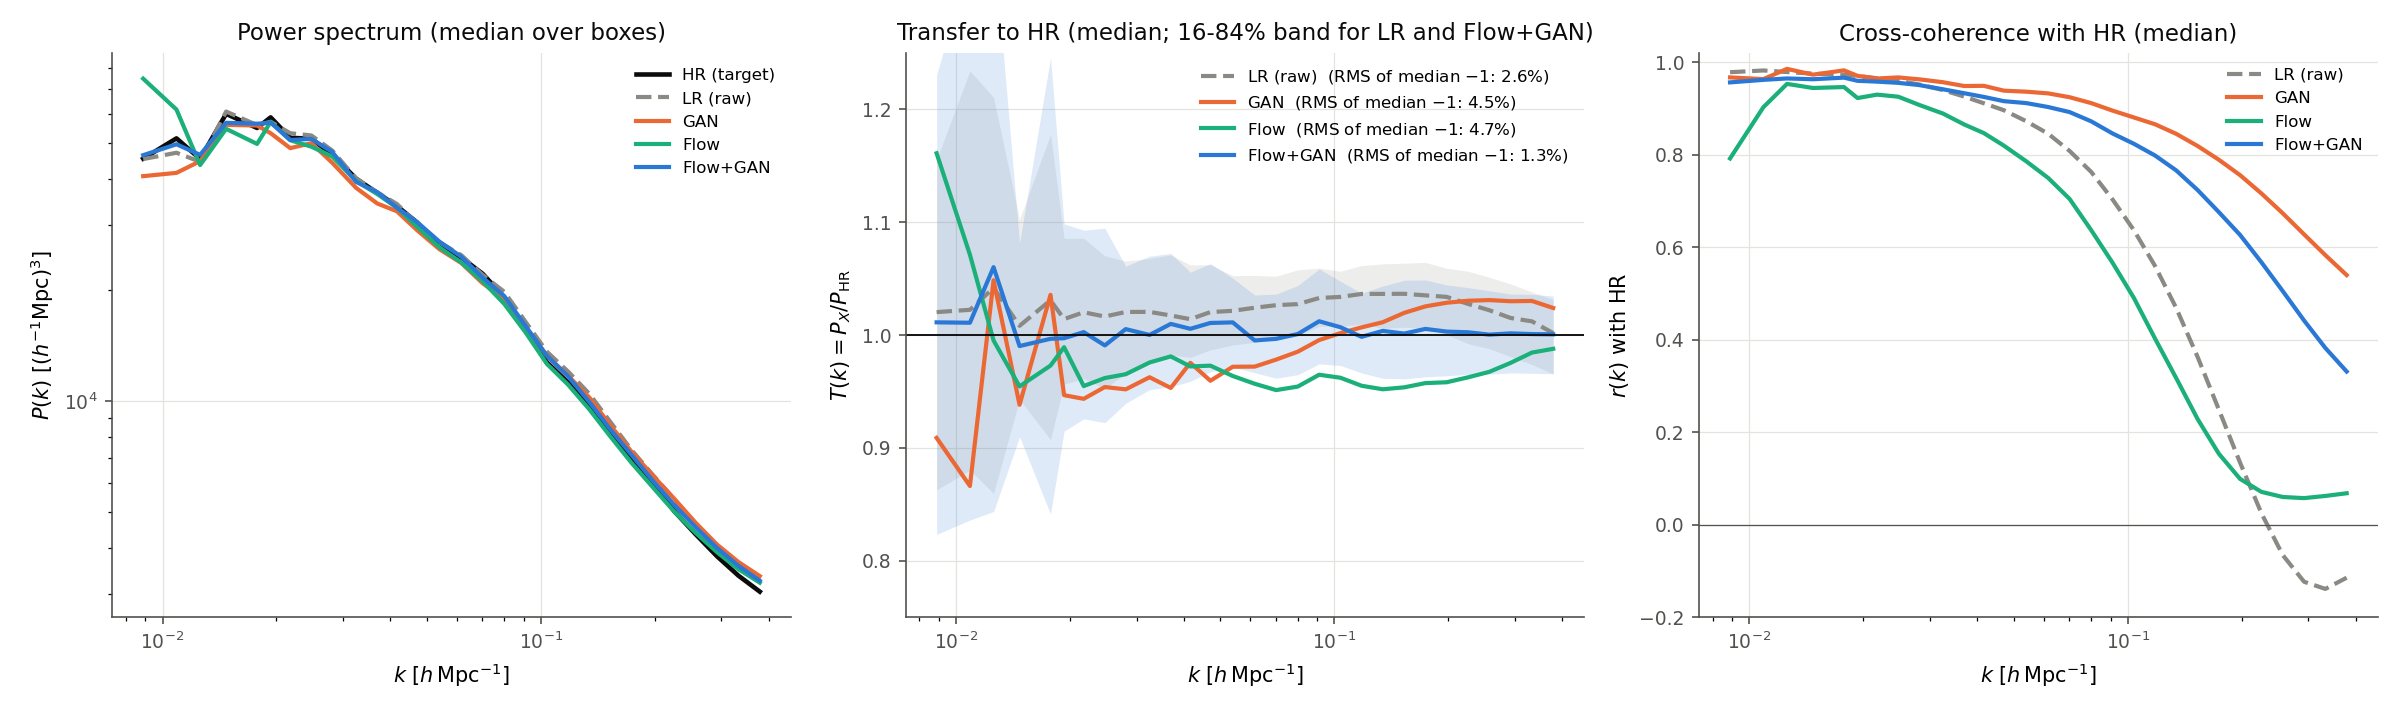
\includegraphics[width=\linewidth]{figures_cmass/pk_panel_box_flowgan.png}
\caption{Full-box diagnostic on $100$ validation boxes. Flow+GAN has no
test-split fields yet, and the first $16$ validation boxes (in sorted order)
were used for checkpoint selection, so we use the next $100$.
\textbf{Left:} median $P(k)$ of HR, LR, GAN, Flow and Flow+GAN.
\textbf{Middle:} transfer $T(k)=P_X/P_\text{HR}$, median, with the 16 to 84
percentile band for LR and Flow+GAN; the legend gives the RMS deviation of the
median from $1$. The GAN (orange) is low at large scales and high at small
scales; the Flow (green) is low at all scales; Flow+GAN (blue) stays on $1$.
\textbf{Right:} cross-coherence $r(k)$ with HR. Flow+GAN is above LR from
$k\approx0.05$ onward and below the deterministic GAN.}
\label{fig:fg-pk}
\end{figure}

\begin{table}[t]
\centering
\caption{Scale by scale, the first $100$ validation boxes, in wide $k$ bands
centred on the listed values. $P/P_\text{HR}$: median power
ratio to HR ($1$ is right). Scatter: box-to-box standard deviation of that ratio
(LR is the reference). $r$: median cross-coherence with HR ($1$ is best).}
\label{tab:fg-scale}
\small
\begin{tabular}{l cccc cc cccc}
\toprule
 & \multicolumn{4}{c}{$P/P_\text{HR}$ median} & \multicolumn{2}{c}{scatter} & \multicolumn{4}{c}{$r$ with HR} \\
\cmidrule(lr){2-5}\cmidrule(lr){6-7}\cmidrule(lr){8-11}
$k$ [$h\,\mathrm{Mpc}^{-1}$] & $0.013$ & $0.042$ & $0.125$ & $0.35$ & $0.013$ & $0.125$ & $0.013$ & $0.042$ & $0.125$ & $0.35$ \\
\midrule
LR (raw)  & $1.009$ & $1.017$ & $1.037$ & $1.007$ & $\mathbf{0.20}$ & $0.34$ & $\mathbf{0.975}$ & $0.908$ & $0.508$ & $-0.126$ \\
GAN       & $0.949$ & $0.962$ & $1.010$ & $1.029$ & $\mathbf{0.20}$ & $0.34$ & $0.974$ & $\mathbf{0.944}$ & $\mathbf{0.850}$ & $\mathbf{0.559}$ \\
Flow      & $1.057$ & $0.970$ & $0.959$ & $0.989$ & $0.40$ & $\mathbf{0.32}$ & $0.907$ & $0.837$ & $0.358$ & $0.062$ \\
Flow+GAN  & $\mathbf{0.986}$ & $\mathbf{1.004}$ & $\mathbf{0.998}$ & $\mathbf{1.009}$ & $0.29$ & $0.35$ & $0.964$ & $0.921$ & $0.760$ & $0.339$ \\
\bottomrule
\end{tabular}
\end{table}

\paragraph{2. Cross-fidelity: Flow+GAN matches LR at the summary level and stays near the floor at the field level.}
Figure~\ref{fig:fg-crossfid} and Table~\ref{tab:fg-crossfid} give the goal
metric. At the summary level the $40$-epoch Flow+GAN reaches $0.047\pm0.008$,
against $0.049\pm0.010$ for raw LR. Compared seed by seed (same NDE seed, same HR
reference posterior), the difference from LR averages $-0.001$. It is the first
SR model that is not worse than LR at the summary level: the GAN is at $0.202$
and the Flow at $0.087$. The final checkpoint (epoch $39$) gives $0.055\pm0.011$,
also equal to LR within noise. At the field level Flow+GAN reaches $0.027\pm0.011$,
close to the HR floor ($0.019$), while the LR-trained CNN posterior does not
transfer reliably ($0.47\pm0.78$).

Two cautions apply. First, epochs $38$ and $39$ are neighbouring checkpoints of one
run, yet their summary KLs differ by $0.008$, about one seed standard deviation.
So the fair claim is that Flow+GAN is equal to LR within noise, not that it beats
LR. Second, the $20$-epoch model (epoch $15$) was at $0.065\pm0.011$. The
improvement from longer training is therefore real but modest, and it is of the
same order as the checkpoint-to-checkpoint noise.

\begin{figure}[t]
\centering
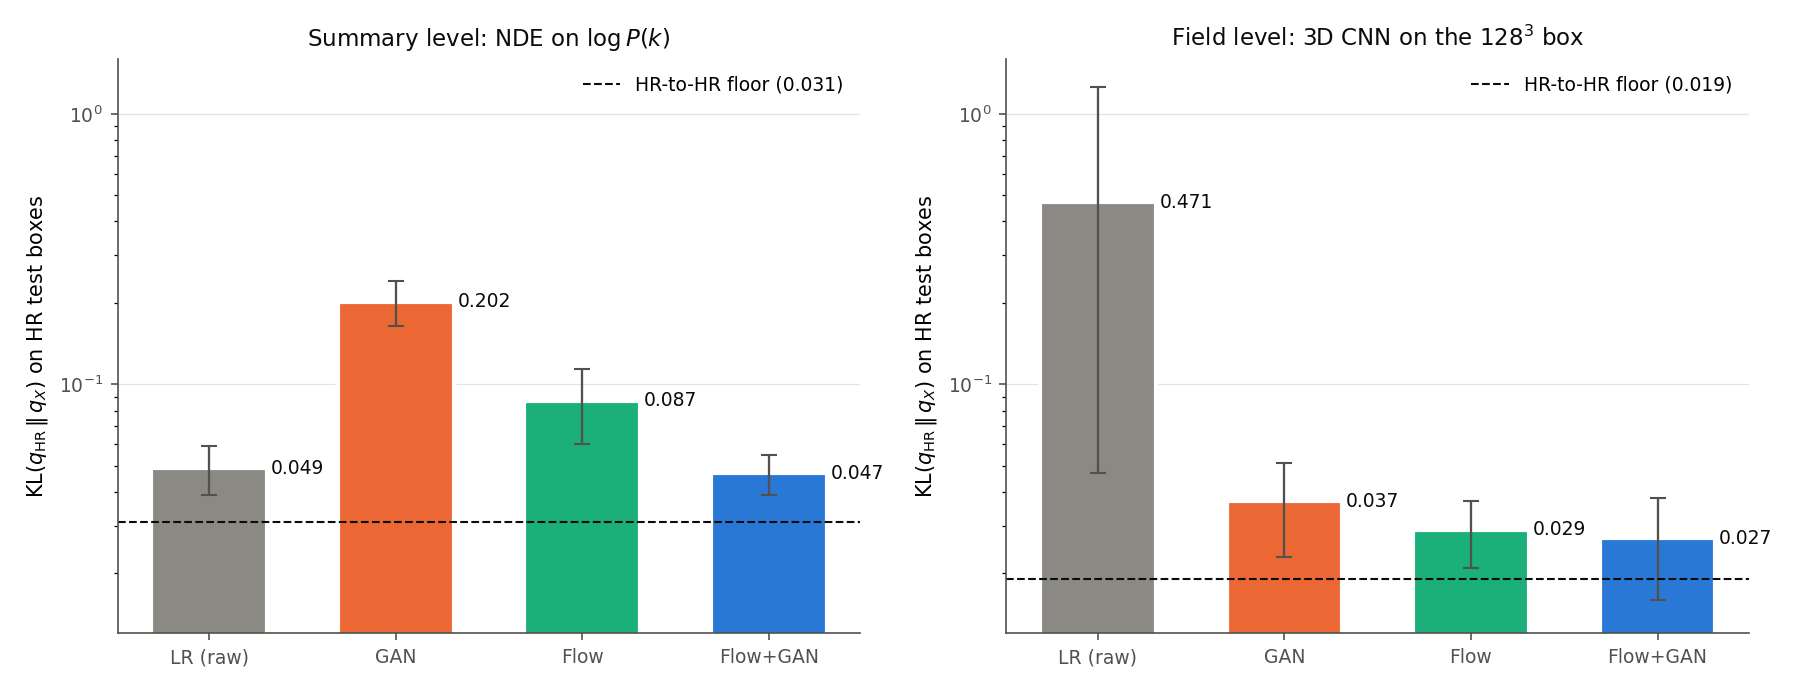
\includegraphics[width=0.95\linewidth]{figures_cmass/crossfid_flowgan.png}
\caption{Cross-fidelity KL to HR (log scale, lower is better), posterior trained
on source $X$ and applied to the $200$ HR test boxes. Dashed: HR-to-HR floor.
Flow+GAN is the $40$-epoch model (CRPS-best checkpoint).
\textbf{Left:} summary level ($P(k)$ NDE, protocol v2, mean $\pm$ std over $8$
seeds). Flow+GAN ($0.047$) equals raw LR ($0.049$); the GAN is at $0.202$ and the
Flow at $0.087$. \textbf{Right:} field level (3D CNN). All three SR models are
near the floor, Flow+GAN ($0.027$) closest; LR does not transfer reliably.}
\label{fig:fg-crossfid}
\end{figure}

\begin{table}[t]
\centering
\caption{Cross-fidelity KL to HR, lower is better. Summary: protocol v2, mean
$\pm$ std over $8$ NDE seeds, $200$ HR test boxes. Field: mean $\pm$ std over
HR-reference $\times$ SR-replicate pairs. Best SR value per column in bold.}
\label{tab:fg-crossfid}
\begin{tabular}{lcc}
\toprule
source & summary $P(k)$ & field (CNN) \\
\midrule
LR (raw, control) & $0.049\pm0.010$ & $0.471\pm0.782$ \\
GAN (deployed)    & $0.202\pm0.038$ & $0.037\pm0.014$ \\
Flow (noise start, patches) & $0.087\pm0.027$ & $0.029\pm0.008$ \\
Flow+GAN, epoch 15 ($20$-epoch run) & $0.065\pm0.011$ & $\mathbf{0.024\pm0.009}$ \\
Flow+GAN, epoch 38 (CRPS-best of $40$) & $\mathbf{0.047\pm0.008}$ & $0.027\pm0.011$ \\
Flow+GAN, epoch 39 (final) & $0.055\pm0.011$ & $0.027\pm0.015$ \\
\midrule
HR floor          & $0.031\pm0.009$ & $0.019$ \\
\bottomrule
\end{tabular}
\end{table}

\paragraph{3. Why it works: the posterior shifts.} Table~\ref{tab:fg-s8}
measures directly how each SR-trained posterior differs from the HR-trained one.
For each HR test box and seed we take the SR-trained posterior mean minus the
HR-trained posterior mean, in units of the HR posterior's standard deviation. We
report the mean over boxes (bias) and the standard deviation over boxes (scatter),
averaged over the $8$ seeds, for the two parameters the $P(k)$ posterior
constrains best, $\Omega_m$ and $\sigma_8$. The GAN's problem is a single one:
its $\sigma_8$ is biased by a full posterior width. After $20$ epochs Flow+GAN has
no such bias beyond LR's own ($+0.23$ vs $+0.18$), but its $\Omega_m$ scatter is
larger than LR's ($0.22$ vs $0.17$). After $40$ epochs the $\sigma_8$ bias is gone
($-0.01$) and the $\Omega_m$ scatter has dropped to $0.18$, close to LR. The same
pattern holds for $n_s$ (scatter $0.34\to0.30$, LR $0.27$). These are the changes
that close the summary gap. The per-box scatter of $\sigma_8$ was never the
problem: it is at LR's level for every Flow+GAN checkpoint. The final checkpoint
(epoch $39$) has a $\sigma_8$ bias of $+0.17$, which is again LR's level, which
shows how much this quantity moves between neighbouring checkpoints.

\begin{table}[h]
\centering
\caption{Shift of the posterior mean on HR test boxes (SR-trained minus
HR-trained), in units of the HR posterior standard deviation; $200$ boxes
$\times$ $8$ seeds. Bias is the mean over boxes, scatter the standard deviation
over boxes. $0$ is ideal for all columns.}
\label{tab:fg-s8}
\begin{tabular}{lcccc}
\toprule
 & \multicolumn{2}{c}{$\Omega_m$} & \multicolumn{2}{c}{$\sigma_8$} \\
\cmidrule(lr){2-3}\cmidrule(lr){4-5}
source & bias & scatter & bias & scatter \\
\midrule
LR (raw)  & $+0.01$ & $\mathbf{0.17}$ & $+0.18$ & $0.38$ \\
GAN (deployed) & $-0.11$ & $0.18$ & $+1.06$ & $0.52$ \\
Flow (patches) & $+0.02$ & $0.21$ & $-0.10$ & $0.46$ \\
Flow+GAN, epoch 15 & $-0.02$ & $0.22$ & $+0.23$ & $0.39$ \\
Flow+GAN, epoch 38 & $+0.03$ & $0.18$ & $\mathbf{-0.01}$ & $0.37$ \\
Flow+GAN, epoch 39 & $+0.01$ & $0.18$ & $+0.17$ & $\mathbf{0.36}$ \\
\bottomrule
\end{tabular}
\end{table}

\paragraph{4. Distribution checks beyond the posterior.} We also ran the
field-level checks of \S\ref{sec:srs} on the $40$-epoch model.
\begin{itemize}
  \item \textbf{PQMass} ($200$ validation boxes, one-point count histogram, as in
  \S\ref{sec:srs}). Flow+GAN at epoch $38$ gives $\chi^2/\text{dof}=1.20$, against
  $0.83$ for LR and $2.22$ for the GAN, so its one-point distribution is close to
  statistically indistinguishable from HR. The $20$-epoch model failed this test
  ($3.59$). We traced that failure to the flow itself: at a fixed total halo count
  it produced about $2\%$ too few cells with two halos and too many with three, and
  $3$ times too many cells with more than $20$ halos. The decoder was not the cause:
  rounding in log space instead of count space changed nothing ($3.65$), and
  thresholds matched to HR's histogram on training boxes moved the total count by
  $9\%$ on validation boxes. After $40$ epochs the excess of very dense cells is
  $1.6\times$ HR's and a small integer-level wobble remains ($0.86$ to $0.98$ of HR
  in the $2$ to $4$ halo bins), but its sign flipped relative to epoch $15$. We read
  it as training noise near the integer lattice, not as a fixed feature. One
  caveat applies when reading any PQMass value here: LR and HR boxes share initial
  conditions, so the two samples are paired rather than independent, and the test
  under-rejects (LR's $p$-values pile up near $1$). A failure is therefore real,
  and a pass is somewhat generous.
  \item \textbf{Bispectrum} ($32$ test boxes, equilateral triangles at
  intermediate $k$). $B/B_\text{HR}=1.106$, the same as LR ($1.112$). The
  $20$-epoch model was at $1.056$. The bispectrum is not an input to either
  posterior.
  \item \textbf{Total halo count.} Mean per-box deficit relative to HR $-1.4\%$
  (LR $-1.9\%$). The robust box-to-box scatter of $\log(N_X/N_\text{HR})$ on the
  test boxes is $0.022$ for LR, the GAN and Flow+GAN alike ($0.0223$, $0.0229$ and
  $0.0216$), so the extra $\Omega_m$ scatter of the $20$-epoch model did not come
  from the total count.
  \item \textbf{Calibration of draws} ($60$ validation boxes $\times$ $8$ draws).
  The spread-skill ratio of $P(k)$ is $0.15$ (ideal $1$) at both epoch $15$ and
  epoch $38$, and the rank histograms are U-shaped at intermediate and high $k$.
  Different draws for the same LR box differ much less than any one draw differs
  from HR. The draws should therefore not be used as a calibrated uncertainty.
  This does not enter the cross-fidelity numbers, which use one draw per box.
\end{itemize}

\paragraph{5. What did not help.} We tested two more ideas aimed at the
large-scale modes, and a third is the one from the previous version of this section.
\begin{itemize}
  \item \textbf{Low-$k$ guidance during sampling} (\texttt{FGguide}, epoch $15$
  model). At every integration step we predict the end point
  $\hat x_1 = x + (1-t)\,v$, pull its Fourier modes toward LR's with a weight that
  is $1$ below $k_1=0.02$ and falls smoothly (cosine) to $0$ at $k_2=0.05\,h\,\mathrm{Mpc}^{-1}$,
  and correct the velocity to match. This is a data-consistency step in the spirit
  of DDNM (Wang et al.\ 2022, arXiv:2212.00490). The $k=0$ mode (total count) is
  never changed. It did what it was designed to do: the box-to-box scatter of
  $P/P_\text{HR}$ at $k<0.03$ fell from $0.41$ to $0.35$ (LR $0.30$), and the
  coherence there rose to LR's. But the summary KL did not move ($0.069\pm0.020$
  vs $0.065\pm0.011$), and the field KL was unchanged ($0.027$). This showed that
  the large-scale scatter was not what separated Flow+GAN from LR, which the
  posterior-shift table then confirmed.
  \item \textbf{Hard low-$k$ swap keeping the total count} (\texttt{*LK3}). The
  previous hard swap (replace all modes $k<0.05$ with LR's) also replaced the $k=0$
  mode, that is the box's total halo count, with LR's. Keeping the model's own
  count helps every model a little (GAN $0.106\to0.084$, Flow+GAN at epoch $15$
  $0.088\to0.075$), but the swap still hurts every flow compared with no swap
  (Flow+GAN at epoch $15$: $0.065\to0.075$; with the original swap the $40$-epoch
  checkpoints go from $0.047$ and $0.055$ to $0.075$ and $0.072$). The posterior
  shifts show why: splicing LR's large-scale modes onto the flow's small scales
  makes the large-to-small-scale power ratio noisier from box to box, and the
  $\sigma_8$ scatter of the epoch-$15$ model rises from $0.39$ to $0.62$.
  \item \textbf{Other decoders.} See the PQMass item above.
\end{itemize}

\subsection{Diagnostic: What is NOT Working}

\paragraph{The draws are under-dispersed.} The spread-skill ratio is $0.15$ and
did not change with longer training. For each LR box the model produces draws that
are too similar to each other, given how far each is from HR. For the
cross-fidelity protocol this does not matter, because we use one draw per box and
compare distributions over boxes. It would matter for any use of several draws as
an error bar. Possible remedies, both untested here, are a stochastic (SDE)
sampler with extra noise and a larger source noise scale at training time.

\paragraph{Checkpoint noise is as large as the remaining effects.} Neighbouring
checkpoints differ by $0.008$ in summary KL and by $0.17$ posterior widths in
$\sigma_8$ bias. Any further improvement of that size needs several checkpoints or
training seeds to be believed.

\paragraph{The hard low-$k$ lock and the low-$k$ guide do not help.} See item 5
of \S\ref{sec:fg-results}. Both act on the large-scale scatter, which turned out
not to be the limiting factor.

\paragraph{Open caveats.} (i) One training run and one seed. A second training
seed would show how stable $0.047$ is; the spread between epochs $38$ and $39$
suggests about $\pm0.008$. (ii) Boxes $0$ to $15$ of the validation split were used
for checkpoint selection and are also among the $200$ PQMass boxes. The
cross-fidelity numbers and Figure~\ref{fig:fg-pk} use only the $200$ test boxes.
(iii) Flow+GAN inherits the GAN's fiducial-cosmology input. A $\theta$-free GAN (for
example the scrambled-label model, summary $0.087$) as the start point is
untested. (iv) The pure-noise full-box control was selected at epoch $2$ by the
pre-registered CRPS rule and later became unstable. Its numbers ($1.19$ summary,
$0.046$ field) are therefore pessimistic, and it does not isolate the benefit of
the GAN start as cleanly as a converged control would.

\subsection{Summary of All Methods and Ablations}
\label{sec:flowgan-ablations}

Tables~\ref{tab:fg-abl-gan} and~\ref{tab:fg-abl-flow} list every model and
ablation we trained on this data, what each one changed, and how it did on the
goal metric. Summary-level numbers all use protocol v2 (\S\ref{sec:fg-eval}), so
every row in the summary column is directly comparable. Rows marked $^8$ use $8$
NDE seeds; the others use $4$. The reference points are raw LR at $0.049$ and the
HR floor at $0.031$. Field-level numbers use the same
HR reference CNNs throughout (floor $0.019$, LR $0.47$). ``n/r'' means not run.
Rows with a \abgood{Good} verdict are the results we would keep. The GAN rows
marked ``scrambled $\theta$'' were trained before the label fix of
\S\ref{sec:srs-correction}. Their cosmology input was effectively noise, so they
behave as unconditioned generators.

\begin{table}[p]
\centering
\caption{Methods and ablations, part 1: raw baselines, GAN variants
(\S\ref{sec:srs}) and evaluation-protocol checks. KL to HR, lower is better.
Summary: protocol v2, mean $\pm$ std over $4$ seeds ($8$ where marked $^8$).
Field: 3D CNN. Good results highlighted.}
\label{tab:fg-abl-gan}
\footnotesize
\begin{tabular}{p{2.5cm}p{5.3cm}ccp{3.6cm}}
\toprule
model (tag) & what changed & summary KL & field KL & verdict \\
\midrule
\multicolumn{5}{l}{\textit{Reference points}} \\
HR floor & HR-trained posterior vs another HR-trained posterior & $0.031\pm0.009^8$ & $0.019$ & best achievable \\
LR, raw CHARM & no model; posterior trained on LR & $0.049\pm0.010^8$ & $0.471\pm0.782$ & control. Tied with Flow+GAN at summary level; unreliable at field level (2 of 8 CNN seeds fail) \\
\midrule
\multicolumn{5}{l}{\textit{GAN, original protocol (with power-spectrum loss)}} \\
Arm A naive (\texttt{cmassA\_naive}) & pad $0$, $\lambda_\text{pk}{=}2$, select on $P(k)$ RMS; scrambled $\theta$ & $0.153\pm0.043$ & n/r & Bad \\
Arm B overlap (\texttt{cmassB\_overlap}) & as Arm A with pad $8$ (real neighbour context) & $0.344\pm0.038$ & n/r & Bad, worst GAN \\
\midrule
\multicolumn{5}{l}{\textit{GAN, new protocol (power-spectrum loss off, select on $L_1$)}} \\
No-$P(k)$ Arm A (\texttt{Anopk}) & Arm A with $\lambda_\text{pk}{=}0$; scrambled $\theta$ & $0.087\pm0.012$ & $\mathbf{0.022\pm0.010}$ & \abgood{Good}: best GAN at summary level; field at floor \\
Lower LR (\texttt{Alowlr}) & \texttt{Anopk} resumed at epoch $15$ with learning rate halved to $5{\times}10^{-5}$ & $0.268\pm0.031$ & n/r & Bad: better $L_1$, worse goal metric \\
Trim-aware pad (\texttt{Baware}) & pad $8$, loss only on the kept $64^3$ core & $0.152\pm0.019$ & n/r & Bad: padding does not help \\
Trim-unaware pad (\texttt{Bunaware}) & pad $8$, loss on the whole $80^3$ output & $0.219\pm0.102$ & n/r & Bad: worst padding variant, unstable \\
\midrule
\multicolumn{5}{l}{\textit{GAN with correct cosmology labels}} \\
Deployed GAN (\texttt{Afixfid}) & retrained with correct $\theta$; sampled at fiducial $\theta$ & $0.202\pm0.038^8$ & $0.037\pm0.014$ & Mixed: field near floor, summary $4{\times}$ LR ($\sigma_8$ bias) \\
Oracle $\theta$ (\texttt{Afixtrue}) & same model, sampled at each box's true $\theta$ (not deployable) & $0.197\pm0.031$ & $0.024\pm0.011$ & Bad at summary level; $\theta$ leak \\
Loss rebalance, Arm R (\texttt{stage0\_R}) & fine-tune deployed GAN $5$ epochs, $\lambda_\text{rec}$ $2\to0.5$ & $0.167\pm0.023$ & n/r & Mixed: fixes 1-point distribution (PQMass $2.22\to0.75$), summary unchanged \\
Smoothed $L_1$, Arm S (\texttt{stage0\_S}) & fine-tune with $L_1$ on a $1.5$-voxel Gaussian-smoothed field & n/r & n/r & Bad: failed the screening checks, not taken further \\
\midrule
\multicolumn{5}{l}{\textit{Post-hoc $P(k)$ tests on the deployed GAN (diagnostics, not new models)}} \\
Regenerated (\texttt{AfixRe}) & same model, fields generated again on the new cluster & $0.194\pm0.033$ & n/r & reproduces $0.185$ \\
Fixed calibration (\texttt{Afixfidcal}) & multiply training $P(k)$ by one fixed per-$k$ curve & $\mathbf{0.068\pm0.010}$ & n/r & \abgood{Good}: proves the GAN's gap is a $P(k)$ tilt \\
Low-$k$ lock (\texttt{AfixLK2}) & replace modes $k<0.05$ with LR's & $0.106\pm0.031$ & n/r & Partial: halves the $\sigma_8$ bias \\
Low-$k$ lock, own count (\texttt{AfixLK3}) & as \texttt{AfixLK2} but keep the GAN's own $k{=}0$ mode (total count) & $0.084\pm0.012$ & n/r & Partial: best GAN post-hoc fix after calibration \\
\midrule
\multicolumn{5}{l}{\textit{Evaluation protocol}} \\
NDE $300$ epochs & NDE trained $300$ instead of $100$ epochs (old 32-bin input) & LR $0.067$, GAN $0.217$ & -- & no gain; keep $100$ \\
\bottomrule
\end{tabular}
\end{table}

\begin{table}[p]
\centering
\caption{Methods and ablations, part 2: flow-matching models and Flow+GAN.
Same columns and protocol as Table~\ref{tab:fg-abl-gan}. Unless noted, flows
are trained on $64^3$ patches with the pure-noise (Gaussian) source. Good
results highlighted.}
\label{tab:fg-abl-flow}
\footnotesize
\begin{tabular}{p{2.5cm}p{5.3cm}ccp{3.6cm}}
\toprule
model (tag) & what changed & summary KL & field KL & verdict \\
\midrule
\multicolumn{5}{l}{\textit{Flow matching on patches}} \\
Flow, dequantised (\texttt{fm\_gauss}) & Gaussian source; uniform dequantisation, floor decoder & $0.244\pm0.107$ & $0.028\pm0.014$ & Bad: spurious halos near empty cells ($+9\%$ count) \\
Flow (\texttt{fm\_gauss\_nodq}) & no dequantisation, rounding decoder & $0.087\pm0.027^8$ & $0.029\pm0.008$ & \abgood{Good}: no $\sigma_8$ bias; best model before Flow+GAN ($0.074$ with $4$ seeds) \\
Flow, regenerated (\texttt{fmRe}) & same model, fields generated again & $0.072\pm0.006$ & n/r & reproduces $0.074$ \\
LR-start flow (\texttt{fm\_lfspec\_nodq}) & source $=$ LR $+$ noise coloured to the residual $P(k)$ & $0.145\pm0.012$ & $0.025\pm0.011$ & Bad at summary level ($\sigma_8$ bias $-0.66$) \\
Late-$t$ emphasis (\texttt{tlate}) & $t$ drawn from a logit-normal shifted toward $t{=}1$ & n/r & n/r & Bad: $6\%$ too many halos; failed screening \\
Dense-region weight (\texttt{lw2}) & loss weighted by $1+2\times$ local LR density & n/r & n/r & Bad: large-scale power $0.875$, coherence below LR; failed screening \\
\midrule
\multicolumn{5}{l}{\textit{Sampling changes (same patch-trained checkpoints)}} \\
Full-box sampling (\texttt{fmFull}) & sample the Flow on the whole $128^3$ box instead of $8$ patches & $0.088\pm0.018$ & $0.026\pm0.010$ & Mixed: coherence at $k{=}0.125$ $0.36\to0.67$; KL same within noise \\
LR-start, full box (\texttt{lfsFull}) & sample \texttt{fm\_lfspec\_nodq} on the full box & $0.119\pm0.008$ & $0.028\pm0.010$ & Bad (better than its patch version, $0.145$) \\
Low-$k$ lock on flows (\texttt{*LK2}) & replace modes $k<0.05$ with LR's after sampling & $0.163$ to $0.244$ & n/r & Bad: hard cut creates a step in $P(k)$ \\
Low-$k$ lock, own count (\texttt{fmLK3}) & as \texttt{fmLK2} but keep the flow's own total count & $0.150\pm0.031$ & n/r & Bad \\
\midrule
\multicolumn{5}{l}{\textit{Full-box training (this section)}} \\
Noise start, full box (\texttt{Flow\_noise\_fullbox}) & Gaussian source, trained on full boxes (control for Flow+GAN) & $1.19\pm0.82$ & $0.046\pm0.012$ & Bad; pessimistic (epoch-2 checkpoint, unstable later) \\
Flow+GAN, $20$ epochs (\texttt{FlowGAN}, epoch 15) & source $=$ frozen GAN output $+\,\sigma_z$ white noise; LR and GAN as conditioning; full box; CRPS selection & $0.065\pm0.011^8$ & $\mathbf{0.024\pm0.009}$ & Good: no GAN $\sigma_8$ bias; fails PQMass ($3.59$) \\
\textbf{Flow+GAN, $40$ epochs} (\texttt{FGcrps40}, epoch 38) & same run resumed to $40$ epochs; CRPS-best checkpoint & $\mathbf{0.047\pm0.008^8}$ & $0.027\pm0.011$ & \abgood{Good}: equal to LR at summary level, near floor at field level; PQMass $1.20$ \\
Flow+GAN, final (\texttt{FGfinal40}, epoch 39) & last checkpoint of the same run & $0.055\pm0.011^8$ & $0.027\pm0.015$ & \abgood{Good}: equal to LR within noise; shows checkpoint noise \\
Flow+GAN $+$ low-$k$ guide (\texttt{FGguide}) & epoch 15; LR's modes imposed smoothly ($k<0.02$, taper to $0.05$) during sampling & $0.069\pm0.020^8$ & $0.027\pm0.006$ & Neutral: large-scale scatter down, KL unchanged \\
Flow+GAN $+$ low-$k$ lock (\texttt{FlowGANLK2}) & epoch 15; replace modes $k<0.05$ with LR's after sampling & $0.088\pm0.010$ & n/r & Bad \\
Flow+GAN $+$ lock, own count (\texttt{FlowGANLK3}) & as above, keeping the model's own total count & $0.075\pm0.005$ & n/r & Bad: less harmful, still worse than no lock \\
Flow+GAN $40$ ep.\ $+$ lock (\texttt{FGcrps40LK}) & epoch 38; original lock & $0.075\pm0.008$ & n/r & Bad \\
Decoder variants (epoch 15) & round in log space; HR-matched thresholds & -- & -- & Bad: PQMass $3.65$; count $+9\%$ \\
\bottomrule
\end{tabular}
\end{table}

\paragraph{What the tables say.} Three results hold across the whole set.
First, nothing we did to the GAN's architecture or loss (padding, learning rate,
loss rebalance, conditioning) brought its summary KL below $0.087$. A fixed
calibration curve did ($0.068$), which showed the gap was a smooth $P(k)$ tilt
rather than lost information. Second, a flow matcher removes that tilt, but
started from noise it loses large-scale coherence. Changing its sampling or its
time and loss emphasis did not fix this. Third, starting the flow from the GAN
keeps the GAN's large scales and the flow's unbiased small scales. Trained for
$40$ epochs, Flow+GAN equals raw LR at the summary level ($0.047$ vs $0.049$) and
stays near the HR floor at the field level ($0.027$ vs $0.019$), where LR is
unreliable. It is the only model we trained that is at least as good as LR on both
levels. Post-hoc changes to the large scales (hard lock or smooth guide) never
helped a flow.

\paragraph{Next step.} The main open issues are the under-dispersed draws and
the checkpoint noise. The first needs a sampler or training change aimed at
calibration; the second needs a second training seed. Replacing the
fiducial-cosmology GAN by a $\theta$-free start point is the remaining design
question.

\subsection{Files}
\begin{itemize}\itemsep0pt
  \item Flow matching package: \texttt{flow\_matching/} (\texttt{README.md} for the
  full ablation design)
  \item Model space and decoder: \texttt{flow\_matching/space.py}
  \item Sources, path, samplers, low-$k$ projection: \texttt{flow\_matching/interpolant.py}
  (source \texttt{gan\_white} is Flow+GAN)
  \item Velocity network: \texttt{flow\_matching/unet3d.py}
  \item Data (patch and full-box, optional GAN channel): \texttt{flow\_matching/data.py};
  augmentations \texttt{flow\_matching/augment.py}
  \item Training: \texttt{flow\_matching/train\_fm.py}; run script
  \texttt{scratch/why/train\_v2\_1gpu.slurm} (multi-GPU:
  \texttt{scratch/why/train\_v2\_ddp.slurm})
  \item Generation and validation metrics: \texttt{flow\_matching/common.py};
  sampling \texttt{flow\_matching/sample\_fm.py}, \texttt{scratch/why/gen\_v2.slurm}
  \item GAN start fields: \texttt{gen\_sr\_fields.py} (deployed GAN at fiducial
  $\theta$, \texttt{sr\_fields/Afix\_fiducial})
  \item Evaluation chain after training: \texttt{scratch/why/post\_v2.sh}
  (generation, $P(k)$, low-$k$ variants, NDEs, summary and field cross-fidelity)
  \item Summary cross-fidelity: \texttt{analysis/seed\_xfid\_check.py},
  \texttt{scripts/crossfid\_reps.slurm}; posteriors in \texttt{runs/patch\_cmass/nde\_v2/}
  \item Field cross-fidelity: \texttt{train\_field\_cnn.py}, \texttt{eval\_field\_crossfid.py},
  \texttt{scratch/why/tier3\_seed.slurm}, \texttt{scratch/why/field\_eval.slurm}
  \item Scale-by-scale power and coherence: \texttt{scratch/why/coh.py}
  (\texttt{COH\_SPLIT=test}), \texttt{scratch/why/epoch\_trend.py};
  posterior shifts: \texttt{scratch/why/post\_diag\_any.py};
  calibration and low-$k$ tests: \texttt{scratch/why/calib.py}, \texttt{scratch/why/lowk.py}
  (\texttt{nodc} keeps the total count)
  \item Low-$k$ guide during sampling: \texttt{flow\_matching/common.py}
  (\texttt{make\_lowk\_guided}), \texttt{sample\_fm.py --lowk-guide 0.02,0.05}
  \item PQMass, bispectrum, halo counts: \texttt{scratch/why/tier1\_any.slurm};
  draw calibration: \texttt{scratch/why/gen\_draws.slurm}, \texttt{scratch/why/spread\_any.slurm};
  decoder study: \texttt{scratch/why/decoder\_study.py}, \texttt{scratch/why/pq\_feat.py}
  \item Figures in this section: \texttt{flow\_matching/plot\_sec7.py}
  $\to$ \texttt{figures\_cmass/pk\_panel\_box\_flowgan.png},
  \texttt{figures\_cmass/crossfid\_flowgan.png}
  \item Checkpoints: \texttt{models/Flow+GAN/best\_crps40\_epoch39.pt} ($40$ epochs,
  CRPS-best, used here), \texttt{epoch\_40.pt} (final),
  \texttt{best\_epoch15\_first20.pt} ($20$-epoch run); SR fields
  \texttt{sr\_fields/Flow+GAN\_crps40/}, \texttt{Flow+GAN\_final40/}, \texttt{Flow+GAN/}
  \item Full log of the $40$-epoch study: \texttt{research\_scratch\_5.md}
\end{itemize}
